% Options for packages loaded elsewhere
\PassOptionsToPackage{unicode}{hyperref}
\PassOptionsToPackage{hyphens}{url}
\PassOptionsToPackage{dvipsnames,svgnames,x11names}{xcolor}
%
\documentclass[
  letterpaper,
  DIV=11,
  numbers=noendperiod]{scrreprt}

\usepackage{amsmath,amssymb}
\usepackage{iftex}
\ifPDFTeX
  \usepackage[T1]{fontenc}
  \usepackage[utf8]{inputenc}
  \usepackage{textcomp} % provide euro and other symbols
\else % if luatex or xetex
  \usepackage{unicode-math}
  \defaultfontfeatures{Scale=MatchLowercase}
  \defaultfontfeatures[\rmfamily]{Ligatures=TeX,Scale=1}
\fi
\usepackage{lmodern}
\ifPDFTeX\else  
    % xetex/luatex font selection
\fi
% Use upquote if available, for straight quotes in verbatim environments
\IfFileExists{upquote.sty}{\usepackage{upquote}}{}
\IfFileExists{microtype.sty}{% use microtype if available
  \usepackage[]{microtype}
  \UseMicrotypeSet[protrusion]{basicmath} % disable protrusion for tt fonts
}{}
\makeatletter
\@ifundefined{KOMAClassName}{% if non-KOMA class
  \IfFileExists{parskip.sty}{%
    \usepackage{parskip}
  }{% else
    \setlength{\parindent}{0pt}
    \setlength{\parskip}{6pt plus 2pt minus 1pt}}
}{% if KOMA class
  \KOMAoptions{parskip=half}}
\makeatother
\usepackage{xcolor}
\ifLuaTeX
  \usepackage{luacolor}
  \usepackage[soul]{lua-ul}
\else
  \usepackage{soul}
  
\fi
\setlength{\emergencystretch}{3em} % prevent overfull lines
\setcounter{secnumdepth}{5}
% Make \paragraph and \subparagraph free-standing
\makeatletter
\ifx\paragraph\undefined\else
  \let\oldparagraph\paragraph
  \renewcommand{\paragraph}{
    \@ifstar
      \xxxParagraphStar
      \xxxParagraphNoStar
  }
  \newcommand{\xxxParagraphStar}[1]{\oldparagraph*{#1}\mbox{}}
  \newcommand{\xxxParagraphNoStar}[1]{\oldparagraph{#1}\mbox{}}
\fi
\ifx\subparagraph\undefined\else
  \let\oldsubparagraph\subparagraph
  \renewcommand{\subparagraph}{
    \@ifstar
      \xxxSubParagraphStar
      \xxxSubParagraphNoStar
  }
  \newcommand{\xxxSubParagraphStar}[1]{\oldsubparagraph*{#1}\mbox{}}
  \newcommand{\xxxSubParagraphNoStar}[1]{\oldsubparagraph{#1}\mbox{}}
\fi
\makeatother


\providecommand{\tightlist}{%
  \setlength{\itemsep}{0pt}\setlength{\parskip}{0pt}}\usepackage{longtable,booktabs,array}
\usepackage{calc} % for calculating minipage widths
% Correct order of tables after \paragraph or \subparagraph
\usepackage{etoolbox}
\makeatletter
\patchcmd\longtable{\par}{\if@noskipsec\mbox{}\fi\par}{}{}
\makeatother
% Allow footnotes in longtable head/foot
\IfFileExists{footnotehyper.sty}{\usepackage{footnotehyper}}{\usepackage{footnote}}
\makesavenoteenv{longtable}
\usepackage{graphicx}
\makeatletter
\def\maxwidth{\ifdim\Gin@nat@width>\linewidth\linewidth\else\Gin@nat@width\fi}
\def\maxheight{\ifdim\Gin@nat@height>\textheight\textheight\else\Gin@nat@height\fi}
\makeatother
% Scale images if necessary, so that they will not overflow the page
% margins by default, and it is still possible to overwrite the defaults
% using explicit options in \includegraphics[width, height, ...]{}
\setkeys{Gin}{width=\maxwidth,height=\maxheight,keepaspectratio}
% Set default figure placement to htbp
\makeatletter
\def\fps@figure{htbp}
\makeatother

\KOMAoption{captions}{tableheading}
\makeatletter
\@ifpackageloaded{bookmark}{}{\usepackage{bookmark}}
\makeatother
\makeatletter
\@ifpackageloaded{caption}{}{\usepackage{caption}}
\AtBeginDocument{%
\ifdefined\contentsname
  \renewcommand*\contentsname{Table of contents}
\else
  \newcommand\contentsname{Table of contents}
\fi
\ifdefined\listfigurename
  \renewcommand*\listfigurename{List of Figures}
\else
  \newcommand\listfigurename{List of Figures}
\fi
\ifdefined\listtablename
  \renewcommand*\listtablename{List of Tables}
\else
  \newcommand\listtablename{List of Tables}
\fi
\ifdefined\figurename
  \renewcommand*\figurename{Figure}
\else
  \newcommand\figurename{Figure}
\fi
\ifdefined\tablename
  \renewcommand*\tablename{Table}
\else
  \newcommand\tablename{Table}
\fi
}
\@ifpackageloaded{float}{}{\usepackage{float}}
\floatstyle{ruled}
\@ifundefined{c@chapter}{\newfloat{codelisting}{h}{lop}}{\newfloat{codelisting}{h}{lop}[chapter]}
\floatname{codelisting}{Listing}
\newcommand*\listoflistings{\listof{codelisting}{List of Listings}}
\makeatother
\makeatletter
\makeatother
\makeatletter
\@ifpackageloaded{caption}{}{\usepackage{caption}}
\@ifpackageloaded{subcaption}{}{\usepackage{subcaption}}
\makeatother
\ifLuaTeX
  \usepackage{selnolig}  % disable illegal ligatures
\fi
\usepackage{bookmark}

\IfFileExists{xurl.sty}{\usepackage{xurl}}{} % add URL line breaks if available
\urlstyle{same} % disable monospaced font for URLs
\hypersetup{
  pdftitle={R-Instat Climatic Guide},
  pdfauthor={Roger Stern, Danny Parsons, David Stern, Francis Torgbor \& James Musyoka},
  colorlinks=true,
  linkcolor={blue},
  filecolor={Maroon},
  citecolor={Blue},
  urlcolor={Blue},
  pdfcreator={LaTeX via pandoc}}

\title{R-Instat Climatic Guide}
\author{Roger Stern, Danny Parsons, David Stern, Francis Torgbor \&
James Musyoka}
\date{2025-01-06}

\begin{document}
\maketitle

\renewcommand*\contentsname{Table of contents}
{
\hypersetup{linkcolor=}
\setcounter{tocdepth}{2}
\tableofcontents
}
\bookmarksetup{startatroot}

\chapter{Acknowledgments}\label{acknowledgments}

\hl{To be added.}

\bookmarksetup{startatroot}

\chapter{About this guide}\label{about-this-guide}

\section{Who is this guide for?}\label{who-is-this-guide-for}

This guide is concerned with the analysis of climatic data. It is for
four types of reader: The first is those concerned with the collection
and subsequent use of their climatic data. This includes staff of
national meteorological services, (NMSs) who are often the custodians of
the historical climatic data for their country. There are many others
who collect climatic data, for example schools and colleges, farms,
agricultural institutes and many individuals.

Second is the users who need results from an analysis of historical
climatic data. They may undertake analyses themselves, or, at least,
need to know what is possible from the data. They are in many walks of
life, including agriculture, health, flood prevention, water supply,
renewable energy, building, tourism and insurance.

The other two groups are concerned more with teaching and learning
statistics. Looking at climatic data is an application of interest to
many people; partly because of the effects that climate has on many
areas. Also because of the many issues of climate change.

So, the third group is those who teach statistics. This guide shows how
simple statistical ideas are used in solving practical problems in one
application area. The key concepts of sensible data handling are the
same whatever the area of application.

The final group consists of those who have to learn statistics. Many
people recognize that they need statistics skills for their work but
sometimes find their statistics courses are difficult to relate to
real-life applications. The materials here are complementary, by
starting with the application and considering the statistical ideas that
are needed to process the data.

These groups overlap. For example, many users of climatic data are also
conscious of their need for further training in statistics.

\section{Why is it needed?}\label{why-is-it-needed}

Many organizations have devoted more effort to collecting climatic data
than to their subsequent analysis. This is like other areas where
monitoring data are collected routinely. One way that climatic data is
perhaps different is that much of the data has an important immediate
use. It is an input for the short-term forecasts and for other immediate
monitoring of the current season. This might be termed a ``spatial
need'' in that these applications benefit from lots of data from
different places at the same time. These data are then stored, and this
guide is for a ``time series need''. Most of the analyses in this guide
are for long records in time. They may be for one, or more, points in
space.

Sometimes the excuse for the lack of analysis is that the quality of the
data is suspect. This is not a good reason, because one way to improve
data quality is to analyze the existing data to demonstrate their
importance and shortcomings.

It is also useful if those who collect data can do their own analysis,
or at least be involved in the analysis. This is highly motivating for
staff and an excellent way to encourage good data quality.

Some familiarity with the use of software (under Windows) is assumed.
Knowledge of statistics is useful, but not essential for most chapters.
Indeed, though this guide cannot substitute for a conventional
statistics book, users can learn many general ideas through seeing where
different techniques are useful.

\section{What software is used?}\label{what-software-is-used}

This guide uses the R Statistical system (R Core Team, 2018). It mainly
uses R through a graphical user interface, called R-Instat. An earlier
version of this guide (Stern, Rijks, Dale, \& Knock, 2006) was for a
simple statistics package, called Instat. Like the original Instat,
R-Instat combines a general statistics package with a special additional
menu to simplify the analysis of climatic data.

R-Instat is designed to support improved learning of statistics in
general as well as providing a wide range of special dialogues to
simplify, and hence facilitate, the analysis of climatic data.

\section{What is in this guide?}\label{what-is-in-this-guide}

Illustrations and `route maps' are provided in all chapters for those
who just wish to study particular topics. We hope that some users will
enjoy the way the ideas unfold in successive chapters but do not assume
that readers will wish to look at every chapter. Most chapters are in a
``tutorial'' style, so readers can follow, and practice at the same
time. There is considerable repetition, to support users to ``dip into''
the chapters they need.

How much practice is needed, depends on the user's current experience in
statistical computing. Those who are relatively inexperienced, or have
never used a statistics package, may be surprised at how easy the ideas
and the software are. However, beginners need practice, so just reading
the guide will not be so effective.

Those with experience of a statistics package should find that R-Instat
is like many other statistics packages. Then practice is not so
important, because they should be able to visualize the results from
just reading the text.

We assume R-Instat has already been installed, see
\href{http://r-instat.org/index.html}{\ul{http://r-instat.org/index.html}}.

Chapters 2 and 3 provide practice of using R-Instat in general. Climatic
data are used, but not the special climatic menu. They assume initial
knowledge of R-Instat that could be from the two initial tutorials.
Beginners should go through these tutorials, while others may just need
to see the corresponding videos.

Chapters 4 to 7 show the use of the R-Instat climatic menu. The
structure of the climatic menu mirrors the main menus. It has items in
the order that is usually needed in an analysis. First is
\textbf{\emph{File}}, to input the data, then \textbf{\emph{Prepare}},
to organise them for analysis, then \textbf{\emph{Describe}}, to analyse
the data without assuming a particular (statistical) model. Lastly, the
menu includes some special modelling items.

If your need is to analyze your own climatic data as quickly as
possible, then you may choose to omit Chapters 2 and 3 initially.
Chapter 4 describes the R-Instat ``climatic system''. This is then
assumed in later chapters. Chapter 5 is on initial exploration of the
data and on quality control. Chapter 6 produces and analyses
``standard'' summaries, such as rainfall totals, while Chapter 7
examines ``tailored products'' such as the start of the rains.

Chapter 8 examines further features of R-Instat, particularly for users
of climatic data who may wish to migrate from R-Instat to using R
itself. There are inevitable limits to the efficient processing of data
with a menu-driven package. This idea is already introduced in Chapter 3
where Section 3.5 is titled ``Don't let the computer laugh at you''.
Hence, for example, Chapter 8 considers how particular climatic analyses
can be done, using tools in R that are currently absent from R-Instat.

The remaining chapters examine more specialised topics. Chapter 9 is on
the input and analysis of gridded satellite and reanalysis data. Chapter
10 is on mapping and 11 introduces the important area of extremes.

The PICSA (Participatory Integrated Climate Services for Agriculture)
project is described briefly in Section 1.6 and in more detail in
Chapter 12.

The remaining chapters are on a range of further topics including the
(statistical approach to) the seasonal forecast, the use of stochastic
models, the processing of within-day data (e.g.~from automatic stations)
and the analysis of circular data, particularly for wind direction.

All the data sets used for illustration are supplied in the R-Instat
``library''. Chapter 3 describes how the data are organized, so readers
can substitute their own data for the examples in later chapters.

The analysis of the climatic records is often a two-stage process. The
first stage reduces the raw, often daily, data to a semi-processed form
with key summaries that correspond to users\textquotesingle{} needs. The
second stage involves processing these summaries.

This two-stage process is typical of the processing of many types of
data and is one reason why users often find their statistics training
did not seem relevant to real-world problems. Many courses use only
small sets of semi-processed data that are tailored to the topic being
taught. However, the real world starts with primary data, and these are
often quite large.

\section{Climatology, statistics, and
computing?}\label{climatology-statistics-and-computing}

Readers who are not confident in statistics should recognize the three
different subjects that are in this guide, namely climatology,
statistics, and computing. The material becomes easier if you separate
these subjects as far as possible.

R is a programming language and those who are already adept in R may
find they do not need the R-Instat menus and dialogues but can use
RStudio more efficiently for the same analyses. In contrast, beginners
in R, sometimes find it difficult to use in their statistics courses.
They are still trying to master the computing ideas, and this becomes
mixed with the statistical objectives.

Computing ideas are raised at various points in this guide, because
users sometimes limit the analyses they conduct, by not exploiting the
software fully. So, we show how R-Instat can be used in different ways,
to solve problems raised by users in their needs for data analysis.
These sections should be recognized as largely computing topics and
perhaps omitted initially by those who have less interest in using R
itself.

Statistics and climatology have two features in common. Both are
relevant to a wide range of applications and many specialists in those
application areas treat both statisticians and climatologists as an
unwelcome nuisance! Perhaps by working together, they can be welcomed
more.

\section{Climate Services for
Agriculture}\label{climate-services-for-agriculture}

Many countries have projects on climate and agriculture. These projects
often concentrate on sharing the information on the short-term and
seasonal forecasts with producers. We outline one such project, called
PICSA (Participatory Integrated Climate Services for Agriculture). More
information on PICSA is here:
\href{https://research.reading.ac.uk/picsa/}{\ul{https://research.reading.ac.uk/picsa/}}.

The different component of PICSA are shown in Fig. 1.6a

\begin{longtable}[]{@{}
  >{\raggedright\arraybackslash}p{(\columnwidth - 0\tabcolsep) * \real{0.9730}}@{}}
\toprule\noalign{}
\begin{minipage}[b]{\linewidth}\raggedright
\textbf{\emph{Fig. 1.6a The PICSA project}}
\end{minipage} \\
\midrule\noalign{}
\endhead
\bottomrule\noalign{}
\endlastfoot
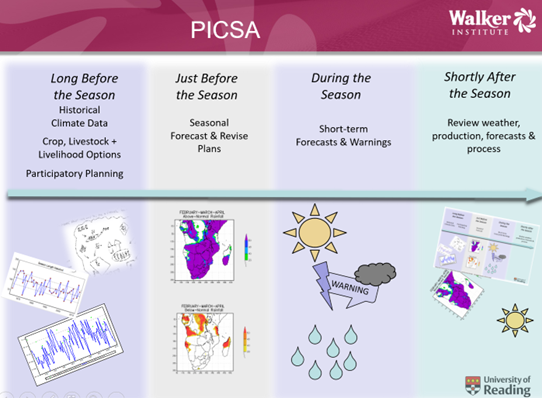
\includegraphics[width=5.64347in,height=4.15038in]{figures/Fig1.6a.png} \\
\end{longtable}

A distinguishing feature of PICSA is the first panel in Fig. 1.6 and
this is in addition to the forecasting activities. The first panel is on
aspects that are based on an analysis of the historical climatic
records, that are shared with small-scale farmers, before the seasonal
forecast is available. The National Met Service (NMS) is a key partner
in each country and provides analyses of the historical data. These
analyses use the methods described in Chapters 6 and 7 of this guide and
are from the climatic stations that are as close as possible to
different groups of farmers. PICSA is described in Chapter 12.

\section{The Climsoft Climate Data Management
System}\label{the-climsoft-climate-data-management-system}

Climsoft is a free and open source system for the entry and management
of primary climatic data. The initial screen is shown in Fig. 1.7a. It
has facilities for the entry and checking of data from paper records,
and for the transfer of data from previous systems, and from automatic
stations. The data, and metadata are currently held in a mysql database.

Climsoft is designed particularly for National Met Services (NMSs), but
can be used by any other organisation that has to manage historical
climatic or other related data. A wide range of elements are
pre-defined, but others can be added for hydrology, pollution or other
aspects. Data can be at any scale, e.g.~daily, 10-minute.

Climsoft includes some products, but not many. Instead, R-Instat can
read data directly from Climsoft, or exported from Climsoft, and is
designed as the products' partner to Climsoft. In later versions of
Climsoft the plan is for some of the R-routines in R-Instat to become
part of Climsoft.

\begin{longtable}[]{@{}
  >{\raggedright\arraybackslash}p{(\columnwidth - 0\tabcolsep) * \real{0.9730}}@{}}
\toprule\noalign{}
\begin{minipage}[b]{\linewidth}\raggedright
\textbf{\emph{Fig. 1.7a The main Climsoft menu}}
\end{minipage} \\
\midrule\noalign{}
\endhead
\bottomrule\noalign{}
\endlastfoot
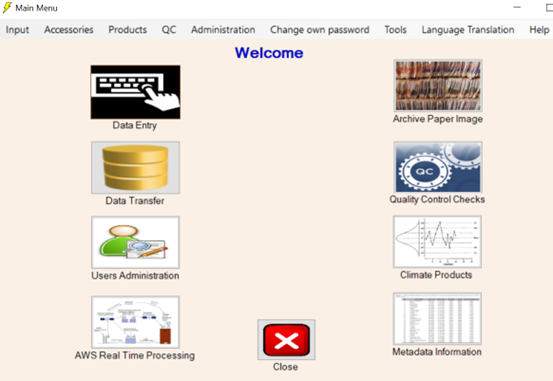
\includegraphics[width=5.75635in,height=3.96937in]{figures/Fig1.7a.png} \\
\end{longtable}

\bookmarksetup{startatroot}

\chapter{More Practice with R-Instat}\label{more-practice-with-r-instat}

\section{Introduction}\label{introduction}

To use climatic data fully it is important to be able to deliver
products. The two examples in this chapter describe the steps and the
endpoint in this process. Data are supplied in the right form for the
analysis. The objectives are specified, and your task is to prepare the
tables and graphs for a report and a presentation.

Some familiarity with R-Instat is assumed. There are two initial
tutorials and following those is enough preparation. If you have already
used a statistics package before, then the examples below may be
sufficient for you, even without the tutorials. This chapter is also
designed to provide practice with R-Instat.

The first problem builds on a study in Southern Zambia. This is the most
drought-prone area of the country. Everyone knew that there is
\textquotesingle climate change\textquotesingle! Some farmers were
emigrating North, citing climate change as their reason. However, a
local non-governmental organization (NGO) called the Conservation
Farming Unit, questioned this reasoning for the rainfall data. They are
not convinced that any climate change has necessarily affected the
farming practices. They, therefore, commissioned a study that used daily
climatic data from several stations in Southern Zambia. The results were
supplied as a report, and presentations of the results were also made to
the NGO and to the local FAO Officers. The results confirmed evidence of
climate change in the temperature data, but not in the rainfall. The key
conclusions were later made into short plays that were broadcast on
local radio and played at village meetings.

Here we use data from Moorings, a site in Southern Zambia. The daily
data, on rainfall, are from 1922 to 2009. Here, partly for simplicity,
we largely use the monthly summaries.

For the work, we draw an analogy with the preparation of a meal. The
first key requirement is that you have the food, which here is the
climatic data. In a real meal, the food may be supplied in a form that
is ready for cooking, or it may need preparation prior to cooking. Here
the data are in pre-packed form, so the analysis can proceed quickly.

You also need the right tools. In a kitchen, they are the saucepans,
etc, while here they are just the computer, together with the required
software.

You need some general cooking skills. These are the basic computing
skills, plus initial skills of R-Instat, at least from the tutorial.

Finally, your objectives must be clear. This corresponds to having a
specific meal in mind so that a recipe can be used. Of course, you may
have to adapt slightly as you go along. You might find some oddities in
the data, just as cooks must improvise if they suddenly find that one of
the ingredients is not available.

If everything is well organized, the cook can prepare the meal very
quickly. This is just what is done in the products in this chapter. This
leaves time to make sure the dishes, for us the results, are presented
attractively. Then users will enjoy consuming what is presented.

Section 2.2 describes the data for this first task. Trends in the
rainfall are examined in Section 2.3. A second problem, in Section 2.4,
examines whether satellite data on sunshine hours resembles
corresponding station data. Daily data from Dodoma, Tanzania, are used.

The data for each of these case studies are in the R-Instat library. The
presentation is designed so users can repeat the analyses on their
laptops.

Graphs are produced in each of these sections and the general methods
for graphics in R-Instat is outlined in Section 2.5. Section 3.5 then
adds a warning. R-Instat provides an easy-to-use click and point way of
using the R programming language. It should help users to solve may
problems. But a click-and-point system is not the right tool for all
problems. We describe a problem that may require more programming
skills, at least if you wish to prevent your computer from laughing at
you!

This chapter demonstrates R-Instat as a simple general statistics
package and the File, Prepare and Describe menus are used. It
illustrates that a general statistics package is an appropriate tool for
many climatic problems. It is also designed to consolidate your
experience in using R-Instat. The special climatic menu is introduced in
chapter 4.

\section{The Moorings data}\label{the-moorings-data}

Monthly data are used in this part of the chapter. Daily data are the
starting point in most of this guide because many of the objectives
require daily data. But here the emphasis is on objectives for which the
monthly data are suitable.

The data are already in an R-Instat file. Hence, they can be opened from
the library in R-Instat library.

From the opening screen in R-Instat, select \textbf{\emph{File
\textgreater{} Open From Library}} as shown in Fig. 2.2a. Choose
\textbf{\emph{Load From Instat Collection}}, Then \textbf{\emph{Browse}}
to the \textbf{\emph{Climatic}} directory then to
\textbf{\emph{Zambia}}. \textbf{\emph{Select}} the file called
\textbf{\emph{Moorings\_July.rds}} to give the screen shown in Fig.
2.2b. Press \textbf{\emph{Ok}}.

\begin{longtable}[]{@{}
  >{\raggedright\arraybackslash}p{(\columnwidth - 2\tabcolsep) * \real{0.5694}}
  >{\raggedright\arraybackslash}p{(\columnwidth - 2\tabcolsep) * \real{0.4167}}@{}}
\toprule\noalign{}
\begin{minipage}[b]{\linewidth}\raggedright
\textbf{\emph{Fig. 2.2a File \textgreater{} Open from Library}}

\textbf{\emph{(Climatic \textgreater{} Zambia \textgreater{}
Moorings.RDS)}}
\end{minipage} & \begin{minipage}[b]{\linewidth}\raggedright
\textbf{\emph{Fig. 2.2b Ready to import Moorings.RDS}}
\end{minipage} \\
\midrule\noalign{}
\endhead
\bottomrule\noalign{}
\endlastfoot
\includegraphics[width=3.35845in,height=3.04612in]{media/image 1404.png}
& \includegraphics{media/image1409.png}\{ width=``2.430002187226597in''
hei ght=``2.7552777777777777in''\} \\
\end{longtable}

The resulting data are shown in Fig. 2.2c. There are 2 data frames. The
one called Moorings has daily data.

\textbf{\emph{Move to the second data frame}} as shown in Fig. 2.2c
which shows the monthly totals. They are the total rainfall in mm and
the total number of rain days. A rain day was defined as a day with more
than 0.85mm\footnote{This threshold is like the value of 1mm sometimes
  suggested by WMO. The smallest value usually recorded is 0.1mm, but we
  find stations are not equally conscientious in recording very small
  amounts. So, if 0.1mm is used, then it is harder to compare the
  pattern of rainfall at different stations. Records also differ in
  their attitudes on rounding. So, some records have far fewer values of
  0.9 or 1.1mm than others. There is also an old issue that some
  stations used to measure in inches and the smallest value was then
  0.01 inches. This translates to 0.3mm and higher values are 0.5, 0.8
  and 1mm. So 0.9mm is not possible in data that used to be in inches.
  Hence the threshold of 0.85mm is a practical way of implementing ``1mm
  and above''.}.

\begin{longtable}[]{@{}
  >{\raggedright\arraybackslash}p{(\columnwidth - 2\tabcolsep) * \real{0.4722}}
  >{\raggedright\arraybackslash}p{(\columnwidth - 2\tabcolsep) * \real{0.5139}}@{}}
\toprule\noalign{}
\begin{minipage}[b]{\linewidth}\raggedright
\textbf{\emph{Fig. 2.2c The Moorings monthly data}}
\end{minipage} & \begin{minipage}[b]{\linewidth}\raggedright
\textbf{\emph{Fig. 2.2d Boxplot dialogue on the Describe menu}}

\textbf{\emph{Describe \textgreater{} Specific \textgreater{} Boxplot}}
\end{minipage} \\
\midrule\noalign{}
\endhead
\bottomrule\noalign{}
\endlastfoot
\includegraphics[width=1.84414in,height=3.4744in]{media/image1423.pn g}
&
\includegraphics[width=3.09565in,height=2.32934in]{media/image141 6.png} \\
\end{longtable}

Rainfall in Southern Zambia is from November to April. Hence, we analyze
the data by season, rather than by year. There are 88 seasons from 1922
to 2009 and 1056 monthly values, as indicated in Fig. 2.2c.

The task is to write a short report that describes the patterns of
rainfall. One aim is to assess whether there is obvious evidence of
change in the pattern of rainfall. This evidence might justify
requesting the data from multiple stations, to undertake a more detailed
study. The first step is to explore the data, and then consider how
appropriate results could be presented. To explore we start with a
boxplot to show the seasonal pattern of the rainfall totals.

Choose the Boxplot dialogue from the Describe menu, with
\textbf{\emph{Describe \textgreater{} Specific \textgreater{} Boxplot}},
as shown in Fog. 2.2d. Complete the dialogue as shown in Fig. 2.2e. The
resulting graph is shown in Fig. 2.2f\footnote{The body of the boxplot
  is not blue by default. For this, choose \textbf{\emph{Boxplot
  Options}} in Fig. 2.2e, then choose the \textbf{\emph{Geom
  Parameters}} tab and change the \textbf{\emph{Fill colour}} to your
  choice.}. This shows the total rainfall was typically 200mm in each of
December to February. There was always some rain in each of these
months, and the records were over 500mm.

\begin{longtable}[]{@{}
  >{\raggedright\arraybackslash}p{(\columnwidth - 2\tabcolsep) * \real{0.5000}}
  >{\raggedright\arraybackslash}p{(\columnwidth - 2\tabcolsep) * \real{0.4861}}@{}}
\toprule\noalign{}
\begin{minipage}[b]{\linewidth}\raggedright
\textbf{\emph{Fig. 2.2e Completed boxplot dialogue}}

\textbf{\emph{Describe \textgreater{} Specific \textgreater{} Boxplot}}
\end{minipage} & \begin{minipage}[b]{\linewidth}\raggedright
\textbf{\emph{Fig. 2.2f Boxplot of monthly rainfall totals}}
\end{minipage} \\
\midrule\noalign{}
\endhead
\bottomrule\noalign{}
\endlastfoot
\includegraphics[width=3.10142in,height=3.54022in]{media/image1413 .png}
&
\includegraphics[width=2.96615in,height=3.09526in]{media/image1424.p ng} \\
\end{longtable}

Change the variable from rain to \textbf{\emph{raindays}} in Fig. 2.2e
to give the corresponding boxplots for the number of raindays in the
month, Fig. 2.2g. This shows that typically one day in two are rainy in
December to February. Occasionally most of the days are rainy.

Boxplots are essentially a 5-number summary of the data, (with potential
outliers also shown). The \textbf{\emph{Prepare \textgreater{} Column:
Reshape \textgreater{} Column Summaries, Fig. 2.2h,}} dialogue can
provide the same summaries numerically.

\begin{longtable}[]{@{}
  >{\raggedright\arraybackslash}p{(\columnwidth - 2\tabcolsep) * \real{0.4912}}
  >{\raggedright\arraybackslash}p{(\columnwidth - 2\tabcolsep) * \real{0.4912}}@{}}
\toprule\noalign{}
\begin{minipage}[b]{\linewidth}\raggedright
\textbf{\emph{Fig. 2.2g The number of rain days}}
\end{minipage} & \begin{minipage}[b]{\linewidth}\raggedright
\textbf{\emph{Fig. 2.2h Summary dialogue on the Prepare menu}}
\end{minipage} \\
\midrule\noalign{}
\endhead
\bottomrule\noalign{}
\endlastfoot
\includegraphics[width=3.2808in,height=3.43955in]{media/image1408.png} &
\includegraphics[width=2.72443in,height=2.69121in]{media/image1421.png} \\
\end{longtable}

Summarise both the monthly totals and the number of raindays, with the
month as the factor, as shown in Fig. 2.2i. Then choose the Summaries
button and complete the sub-dialogue as shown in Fig. 2.2j.

\begin{longtable}[]{@{}
  >{\raggedright\arraybackslash}p{(\columnwidth - 2\tabcolsep) * \real{0.5278}}
  >{\raggedright\arraybackslash}p{(\columnwidth - 2\tabcolsep) * \real{0.4583}}@{}}
\toprule\noalign{}
\begin{minipage}[b]{\linewidth}\raggedright
\textbf{\emph{Fig. 2.2i The Summary dialogue}}

\textbf{\emph{Prepare \textgreater{} Column: Reshape \textgreater{}
Column Summaries}}
\end{minipage} & \begin{minipage}[b]{\linewidth}\raggedright
\textbf{\emph{Fig. 2.2j Summaries sub-dialogue}}
\end{minipage} \\
\midrule\noalign{}
\endhead
\bottomrule\noalign{}
\endlastfoot
\includegraphics[width=3.20563in,height=3.34338in]{media/image107 9.png}
&
\includegraphics[width=2.73372in,height=3.67453in]{media/image1065.png} \\
\end{longtable}

The results are in a third data frame. It just has 12 rows as shown in
Fig. 2.2k. The summaries are clearer if they are in order (which we did
already for Fig. 2.2k).

\textbf{\emph{Right-click in the name field}} of this data frame and
choose the option to \textbf{\emph{Reorder columns}}, Fig. 2.2l.

\begin{longtable}[]{@{}
  >{\raggedright\arraybackslash}p{(\columnwidth - 2\tabcolsep) * \real{0.4912}}
  >{\raggedright\arraybackslash}p{(\columnwidth - 2\tabcolsep) * \real{0.4912}}@{}}
\toprule\noalign{}
\begin{minipage}[b]{\linewidth}\raggedright
\textbf{\emph{Fig. 2.2k Resulting summary data}}
\end{minipage} & \begin{minipage}[b]{\linewidth}\raggedright
\textbf{\emph{Fig 2.2l Right-click menu to reorder columns}}
\end{minipage} \\
\midrule\noalign{}
\endhead
\bottomrule\noalign{}
\endlastfoot
\includegraphics[width=3.51673in,height=2.44292in]{media/image1078.png}
&
\includegraphics[width=2.41931in,height=2.46411in]{media/image1074.png} \\
\end{longtable}

In the Reorder dialogue, use the \textbf{\emph{arrow keys}} to change
the position of the columns in the data frame.

With the summaries in a sensible order, they are now transferred to the
results (output) window.

\begin{longtable}[]{@{}
  >{\raggedright\arraybackslash}p{(\columnwidth - 2\tabcolsep) * \real{0.5000}}
  >{\raggedright\arraybackslash}p{(\columnwidth - 2\tabcolsep) * \real{0.4861}}@{}}
\toprule\noalign{}
\begin{minipage}[b]{\linewidth}\raggedright
\textbf{\emph{Fig. 2.2m Reorder the resulting columns}}

\textbf{\emph{Right-Click \textgreater{} Reorder Column(s)}}
\end{minipage} & \begin{minipage}[b]{\linewidth}\raggedright
\textbf{\emph{Fig. 2.2n Simplify column names}}

\textbf{\emph{Right-click \textgreater{} Rename Column}}
\end{minipage} \\
\midrule\noalign{}
\endhead
\bottomrule\noalign{}
\endlastfoot
\includegraphics[width=3.09828in,height=2.21875in]{media/image1080. png}
&
\includegraphics[width=3.0263in,height=2.08349in]{media/image1077.p ng} \\
\end{longtable}

Before this, we renamed some of the columns to give shorter names. This
again used the \textbf{\emph{right-click}} menu, Fig 2.2l. The rename
dialogue is shown in Fig. 2.2n.

\begin{longtable}[]{@{}
  >{\raggedright\arraybackslash}p{(\columnwidth - 2\tabcolsep) * \real{0.4444}}
  >{\raggedright\arraybackslash}p{(\columnwidth - 2\tabcolsep) * \real{0.5417}}@{}}
\toprule\noalign{}
\begin{minipage}[b]{\linewidth}\raggedright
\textbf{\emph{Fig. 2.2o View Data dialogue}}

\textbf{\emph{Prepare \textgreater{} Data Frame \textgreater{} View
Data}}
\end{minipage} & \begin{minipage}[b]{\linewidth}\raggedright
\textbf{\emph{Fig. 2.2n The Monthly number of rain days}}
\end{minipage} \\
\midrule\noalign{}
\endhead
\bottomrule\noalign{}
\endlastfoot
\includegraphics{media/image1091.png} \{width=``2.7121620734908136in''
height=``2.720417760279965in''\} &
\includegraphics[width=3.3783in,height=2.30157in]{media/image1 075.jpg} \\
\end{longtable}

Now use the \textbf{\emph{Prepare \textgreater{} Data Frame
\textgreater{} View Data}} dialogue, Fig. 2.2o, to transfer the rainfall
totals and then the number of rain days to the results window. The
results for the number of rain days are shown in Fig. 2.2p.

\section{The objectives}\label{the-objectives}

Section 2.2 explored the data and examined the seasonal pattern of the
rainfall at Moorings. It also made use of the three menus, File, Prepare
and Describe and well as the right-click menu. The main objective,
however, was to see if there is evidence of rainfall change rather than
to investigate the seasonal pattern.

We first examine the annual totals and the total number of rain days.
These are the totals from July to June, so they cover each season.

Some ``housekeeping'' is a preliminary. The 3\textsuperscript{rd}
data-frame is no longer needed. Right-click on the bottom tab a and
choose the option to delete, Fig. 2.3a. The dialogue shown in Fig. 2.3b
opens. Just press ok.

\begin{longtable}[]{@{}
  >{\raggedright\arraybackslash}p{(\columnwidth - 2\tabcolsep) * \real{0.3068}}
  >{\raggedright\arraybackslash}p{(\columnwidth - 2\tabcolsep) * \real{0.6818}}@{}}
\toprule\noalign{}
\begin{minipage}[b]{\linewidth}\raggedright
\textbf{\emph{Fig. 2.3a Right-click on the bottom tab}}
\end{minipage} & \begin{minipage}[b]{\linewidth}\raggedright
\textbf{\emph{Fig. 2.3b Delete a data frame}}
\end{minipage} \\
\midrule\noalign{}
\endhead
\bottomrule\noalign{}
\endlastfoot
\includegraphics[width=2.15289in,height=1.68759in]{media/image1086.png}
&
\includegraphics[width=3.80764in,height=2.32324in]{media/image1081.png} \\
\end{longtable}

Use \textbf{\emph{Prepare \textgreater{} Column: Reshape \textgreater{}
Column Summaries}} and complete the dialogue and sub-dialogue as shown
in Fig. 2.3c and Fig. 2.3d to produce the seasonal totals.

\begin{longtable}[]{@{}
  >{\raggedright\arraybackslash}p{(\columnwidth - 2\tabcolsep) * \real{0.5139}}
  >{\raggedright\arraybackslash}p{(\columnwidth - 2\tabcolsep) * \real{0.4722}}@{}}
\toprule\noalign{}
\begin{minipage}[b]{\linewidth}\raggedright
\textbf{\emph{Fig. 2.3c Produce the annual totals}}

\textbf{\emph{Prepare \textgreater{} Column: Reshape \textgreater{}
Column Summaries}}
\end{minipage} & \begin{minipage}[b]{\linewidth}\raggedright
\textbf{\emph{Fig. 2.3d The Summaries sub-dialogue}}
\end{minipage} \\
\midrule\noalign{}
\endhead
\bottomrule\noalign{}
\endlastfoot
\begin{minipage}[t]{\linewidth}\raggedright
\begin{figure}[H]

{\centering \includegraphics[width=3.19367in,height=3.34039in]{media/image1057 .png}

}

\caption{C:\textbackslash Users\textbackslash R
OGERS\textasciitilde1\textbackslash AppData\textbackslash Local\textbackslash Temp\textbackslash SN
AGHTML1b0bb1d.PNG}

\end{figure}%
\end{minipage} &
\includegraphics[width=2.83124in,height=3.80561in]{media/image1048.pn g} \\
\end{longtable}

The results are shown in Fig. 2.3 e after the steps explained below.
First, notice in Fig. 2.3e that there were only 4 months in the first
season, and the annual summary was therefore set to missing\footnote{This
  is partly because the ``Omit Missing Values'' checkbox in Fig. 2.3c
  was left unchecked. Coping with missing values in the data, when
  summaries are calculated, is a complex issue. It is discussed in
  detail in Chapter 6.}.

\begin{longtable}[]{@{}
  >{\raggedright\arraybackslash}p{(\columnwidth - 2\tabcolsep) * \real{0.4912}}
  >{\raggedright\arraybackslash}p{(\columnwidth - 2\tabcolsep) * \real{0.4912}}@{}}
\toprule\noalign{}
\begin{minipage}[b]{\linewidth}\raggedright
\textbf{\emph{Fig. 2.3e Resulting annual data}}
\end{minipage} & \begin{minipage}[b]{\linewidth}\raggedright
\textbf{\emph{Fig. 2.3f Menu for a text substring}}
\end{minipage} \\
\midrule\noalign{}
\endhead
\bottomrule\noalign{}
\endlastfoot
\includegraphics[width=2.94072in,height=3.52182in]{media/image1092.png}
&
\includegraphics[width=3.02793in,height=2.81264in]{media/image1053.png} \\
\end{longtable}

A numeric column for the year (season) is needed for the time series
graphs. Hence, as shown below, we produce the second column, called
s\_yr, also shown in Fig. 2.3e.

Use \textbf{\emph{Prepare \textgreater{} Column: Text \textgreater{}
Transform}}, Fig. 2.3f. Complete the resulting dialogue, as shown in
Fig. 2.3g, to give just the starting year of the season. The resulting
variable is shown in Fig. 2.3e.

\begin{longtable}[]{@{}
  >{\raggedright\arraybackslash}p{(\columnwidth - 2\tabcolsep) * \real{0.5694}}
  >{\raggedright\arraybackslash}p{(\columnwidth - 2\tabcolsep) * \real{0.4167}}@{}}
\toprule\noalign{}
\begin{minipage}[b]{\linewidth}\raggedright
\textbf{\emph{Fig. 2.3g The Substring Option}}

\textbf{\emph{Prepare \textgreater{} Column:Text \textgreater{}
Transform}}
\end{minipage} & \begin{minipage}[b]{\linewidth}\raggedright
\textbf{\emph{Fig. 2.3h Convert Column to Numeric}}
\end{minipage} \\
\midrule\noalign{}
\endhead
\bottomrule\noalign{}
\endlastfoot
\includegraphics[width=3.45986in,height=3.00122in]{media/imag e1056.png}
& \includegraphics{media/image1076.png}\{ width=``2.003675634295713in''
hei ght=``2.8906255468066493in''\} \\
\end{longtable}

Use the \textbf{\emph{right-click}} menu, Fig. 2.3h to convert the
resulting s\_yr column to numeric.

After a little further housekeeping from the right-click menu, to
\textbf{\emph{rename}}, \textbf{\emph{re-orde}}r and
\textbf{\emph{delete}} columns, the annual data are as shown in Fig.
2.3e above.

Now for the time-series graphs. They can be produced using the
\textbf{\emph{Describe \textgreater{} Specific \textgreater{} Line
Plot}} dialogue, but this type of graph is just what is needed for the
PICSA-style rainfall graphs, so we use the special climatic menu for the
first time.

Use \textbf{\emph{Climatic \textgreater{} PICSA \textgreater{} Rainfall
Graph}}. Complete as shown in Fig. 2.3i. Press the \textbf{PICSA
Options} button and complete the Lines ab as shown in Fig. 2.3j to add
(and label) a horizontal line for the mean.

\begin{longtable}[]{@{}
  >{\raggedright\arraybackslash}p{(\columnwidth - 2\tabcolsep) * \real{0.4583}}
  >{\raggedright\arraybackslash}p{(\columnwidth - 2\tabcolsep) * \real{0.5278}}@{}}
\toprule\noalign{}
\begin{minipage}[b]{\linewidth}\raggedright
\textbf{\emph{Fig. 2.3i PICSA Rainfall graph dialogue}}

\textbf{\emph{Climatic \textgreater{} PICSA \textgreater{} Rainfall
Graph}}
\end{minipage} & \begin{minipage}[b]{\linewidth}\raggedright
\textbf{\emph{Fig. 2.3j Add a line showing the mean}}
\end{minipage} \\
\midrule\noalign{}
\endhead
\bottomrule\noalign{}
\endlastfoot
\includegraphics[width=2.79572in,height=2.51954in]{media/image1059.png}
&
\includegraphics[width=3.26365in,height=2.3179in]{media/image10 55.png} \\
\end{longtable}

The resulting graph is shown in Fig 2.3k\footnote{The graph in Fig. 2.4k
  also starts from 0. This used the Yaxis tab in Fig. 2.3j.}.
\textbf{\emph{Return to the dialogue}} and put \textbf{\emph{raindays}}
as the y-variable to give the results in Fig. 2.3l.

\begin{longtable}[]{@{}
  >{\raggedright\arraybackslash}p{(\columnwidth - 2\tabcolsep) * \real{0.4911}}
  >{\raggedright\arraybackslash}p{(\columnwidth - 2\tabcolsep) * \real{0.4911}}@{}}
\toprule\noalign{}
\begin{minipage}[b]{\linewidth}\raggedright
\textbf{\emph{Fig. 2.3k Seasonal rainfall totals}}
\end{minipage} & \begin{minipage}[b]{\linewidth}\raggedright
\textbf{\emph{Fig. 2.3l Number of rain days}}
\end{minipage} \\
\midrule\noalign{}
\endhead
\bottomrule\noalign{}
\endlastfoot
\includegraphics[width=3.01733in,height=1.50165in]{media/image1058.png}
&
\includegraphics[width=2.87199in,height=1.42931in]{media/image1064.png} \\
\end{longtable}

These graphs indicate large inter-annual variability, but they don't
seem to show a trend. That is important because, if you can attribute
your farming problems to climate change, then there may be nothing you
can do. But coping with the variability is what farmers have always had
to do.

With results such as shown in Fig. 2.3k and 2.3l you can start comparing
risks for different options in your farming and in other enterprises.
That sort of idea is discussed in PICSA workshops.

Some may find the graph shown above to be convincing evidence that, with
rainfall, the pressing problem is variability, rather than change. We
stress that there IS climate change, and similar graphs with temperature
data show a trend. If the temperatures have changed, then the ``system''
has changed, and it follows that other elements including rainfall will
be affected. Currently, however, with this sort of analysis, it is
usually not yet possible to determine which way the pattern of rainfall
may change. It is difficult to detect a small change when the
inter-annual variability is so large. And, even if a change is detected,
coping as well as possible with the variability must be a good thing to
do.

Some people are not convinced by graphs such as are shown above. A
common statement is that the annual totals that might still be similar,
but the season is shorter, because planting is delayed, etc. We examine
this in more detail in Chapter 7. There the daily data are used to
define the start, end and length of the season as well as to examine dry
spells and extremes during the season. With the monthly total, the
examination can start by repeating the analysis above, but just for
November and December, when the season starts.

\textbf{\emph{Return to the monthly data frame}} and
\textbf{\emph{filter}} to examine just those months. So, make sure you
are on the monthly data. \textbf{\emph{Right click}} as usual and choose
\textbf{\emph{Filter}}, Fig. 2.3m

\begin{longtable}[]{@{}
  >{\raggedright\arraybackslash}p{(\columnwidth - 2\tabcolsep) * \real{0.2679}}
  >{\raggedright\arraybackslash}p{(\columnwidth - 2\tabcolsep) * \real{0.7225}}@{}}
\toprule\noalign{}
\begin{minipage}[b]{\linewidth}\raggedright
\textbf{\emph{Fig. 2.3m Right-click for Filter}}
\end{minipage} & \begin{minipage}[b]{\linewidth}\raggedright
\textbf{\emph{Fig. 2.3n The filter dialogue}}
\end{minipage} \\
\midrule\noalign{}
\endhead
\bottomrule\noalign{}
\endlastfoot
\includegraphics[width=2.88588in,height=3.65868in]{media/image1104.png}
&
\includegraphics{media/image1106.png}\includegraphics{media/image1106.png}\includegraphics[width=3.24375in,height=3.2541in]{media/image1107.png} \\
\end{longtable}

In Fig. 2.3n, click to \textbf{\emph{Define new Filter}}. Complete the
sub-dialogue as shown in Fig. 2.3o. The steps are as follows:

\begin{enumerate}
\def\labelenumi{\arabic{enumi})}
\item
  \textbf{\emph{Choose the month}} column
\item
  \textbf{\emph{Select Nov and Dec}} as shown in Fig. 2.3p
\item
  Click to \textbf{\emph{Add Condition}}
\item
  Press \textbf{\emph{Return}}
\end{enumerate}

\begin{longtable}[]{@{}
  >{\raggedright\arraybackslash}p{(\columnwidth - 2\tabcolsep) * \real{0.4912}}
  >{\raggedright\arraybackslash}p{(\columnwidth - 2\tabcolsep) * \real{0.4912}}@{}}
\toprule\noalign{}
\begin{minipage}[b]{\linewidth}\raggedright
\textbf{\emph{Fig. 2.3o Defining the filter}}
\end{minipage} & \begin{minipage}[b]{\linewidth}\raggedright
\textbf{\emph{Fig. 2.3p The filtered data}}
\end{minipage} \\
\midrule\noalign{}
\endhead
\bottomrule\noalign{}
\endlastfoot
\includegraphics[width=3.99193in,height=2.85751in]{media/image1135.png}
&
\includegraphics[width=2.05557in,height=2.97506in]{media/image1131.png} \\
\end{longtable}

Back on the main filter dialogue, just \textbf{\emph{press Ok}}. The
data are now as shown in Fig. 2.3p. The first column is in red and this
shows a filter is in operation. Also, at the bottom of the data frame,
you see there are now 176 rows (months) of data to analyse, out of the
original 1062 rows.

The other data have not gone away. If ever you wish to return, then just
press right-click as before, Fig. 2.3m and choose the last option to
\textbf{\emph{Remove Current Filter}}.

Now it is quick to repeat the steps above for this analysis. It is
simpler to recall the last dialogues as shown in Fig. 2.3q.

\begin{longtable}[]{@{}
  >{\raggedright\arraybackslash}p{(\columnwidth - 2\tabcolsep) * \real{0.4912}}
  >{\raggedright\arraybackslash}p{(\columnwidth - 2\tabcolsep) * \real{0.4912}}@{}}
\toprule\noalign{}
\begin{minipage}[b]{\linewidth}\raggedright
\textbf{\emph{Fig. 2.3q Recall the last dialogues}}
\end{minipage} & \begin{minipage}[b]{\linewidth}\raggedright
\textbf{\emph{Fig. 2.3r The Column Statistics dialogue}}
\end{minipage} \\
\midrule\noalign{}
\endhead
\bottomrule\noalign{}
\endlastfoot
\includegraphics[width=2.60356in,height=2.74636in]{media/image1112.png}
&
\includegraphics[width=3.31515in,height=3.4576in]{media/image1130.png} \\
\end{longtable}

The Column Statistics dialogue and sub-dialogue remain completed from
before, Fig. 2.3r. So just \textbf{\emph{press Ok}}.

The new columns have added to the existing annual sheet. So, go straight
to the PICSA Rainfall Graphs dialogue again. \textbf{\emph{Choose the
new variable}} for the November-December totals and press OK. The mean
is now 286mm for the 2 months. Repeat for the number of rain days to
give the graphs for the filtered data, see Fig. 2.3s and 2.3t.

\begin{longtable}[]{@{}
  >{\raggedright\arraybackslash}p{(\columnwidth - 2\tabcolsep) * \real{0.4821}}
  >{\raggedright\arraybackslash}p{(\columnwidth - 2\tabcolsep) * \real{0.5000}}@{}}
\toprule\noalign{}
\begin{minipage}[b]{\linewidth}\raggedright
\textbf{\emph{Fig. 2.3s Rainfall totals Nov-Dec}}
\end{minipage} & \begin{minipage}[b]{\linewidth}\raggedright
\textbf{\emph{Fig. 2.3t Number of rain days Nov-Dec}}
\end{minipage} \\
\midrule\noalign{}
\endhead
\bottomrule\noalign{}
\endlastfoot
\includegraphics[width=2.96668in,height=1.47644in]{media/image1136.png}
&
\includegraphics[width=3.03197in,height=1.50893in]{media/image1120.png} \\
\end{longtable}

One feature of the data in Fig. 2.3s is that had the record started in
1981, then it might have given an impression of an upward trend in the
rainfall total. The longer record shows that this sort of conclusion
should be treated with considerable caution!

These graphs start to satisfy the objective of examining the rainfall
data in Southern Zambia for trends. The results should be considered as
provisional if only because they are from just a single station and only
use the monthly data. We suggest they make a case for a more complete
analysis with multiple stations.

\section{Comparing satellite and station
data}\label{comparing-satellite-and-station-data}

Our proposed objective is to report on the feasibility of using
satellite estimates of sunshine hours to supplement the information from
station data. The station network for sunshine or radiation is sparse in
many countries. Where it exists the records often have many missing
values.

Estimates of daily hours of sunshine are also available from the
EUMETSAT CMSAF (Climate Monitoring Satellite Application Facility) for
about 5km square pixels. The data are available from 1983 and may be
downloaded free of charge. These data are in NetCDF files and examples
from a few locations have been downloaded and are the R-Instat library.

Data from Dodoma, Tanzania was analysed in the second tutorial and the
same dataset is used here. In this exercise, these data are merged with
the corresponding satellite data and the two variables are then
compared.

As in the tutorial use \textbf{\emph{File \textgreater{} Open From
Library}}. Choose the \textbf{\emph{Instat collection}}. Browse to the
\textbf{\emph{Climatic directory}} and choose the \textbf{\emph{Original
Climatic Guide datasets}}. Choose just the \textbf{\emph{Dodoma}} sheet,
Fig. 2.4a.

\begin{longtable}[]{@{}
  >{\raggedright\arraybackslash}p{(\columnwidth - 2\tabcolsep) * \real{0.4911}}
  >{\raggedright\arraybackslash}p{(\columnwidth - 2\tabcolsep) * \real{0.4911}}@{}}
\toprule\noalign{}
\begin{minipage}[b]{\linewidth}\raggedright
\textbf{\emph{Fig. 2.4a Importing the Dodoma data}}
\end{minipage} & \begin{minipage}[b]{\linewidth}\raggedright
\textbf{\emph{Fig. 2.4b Add a Date column}}
\end{minipage} \\
\midrule\noalign{}
\endhead
\bottomrule\noalign{}
\endlastfoot
\includegraphics[width=3.17958in,height=2.6814in]{media/image1083.png} &
\includegraphics[width=2.83037in,height=2.6954in]{media/image1101.png} \\
\end{longtable}

Once imported use \textbf{\emph{Prepare \textgreater{} Column: Date
\textgreater{} Make Date}}, Fig. 2.4b to construct a date column from
the Year, Month, Day columns. Name the resulting column as
\textbf{\emph{Date}}, see Fig. 2.4b.

Now use \textbf{\emph{File \textgreater{} Import and Tidy NetCDF File}},
Fig. 2.4c. Choose the option \textbf{\emph{From Library}} and the file
that starts \textbf{\emph{CMSAF\_SDU}} (for sunshine duration). This
file contains just the data from the nearest pixel to the Dodoma station
data.

\begin{longtable}[]{@{}
  >{\raggedright\arraybackslash}p{(\columnwidth - 2\tabcolsep) * \real{0.6723}}
  >{\raggedright\arraybackslash}p{(\columnwidth - 2\tabcolsep) * \real{0.3164}}@{}}
\toprule\noalign{}
\begin{minipage}[b]{\linewidth}\raggedright
\textbf{\emph{Fig. 2.4c Import the CMSAF satellite data}}
\end{minipage} & \begin{minipage}[b]{\linewidth}\raggedright
\textbf{\emph{Fig. 2.4d Change the name to Date}}
\end{minipage} \\
\midrule\noalign{}
\endhead
\bottomrule\noalign{}
\endlastfoot
\includegraphics[width=2.98774in,height=1.78115in]{media/image1088.png}
&
\includegraphics[width=3.03993in,height=1.77358in]{media/image1085.png} \\
\end{longtable}

Once imported, \textbf{\emph{right-click}} to change the name of the
last column from \textbf{\emph{time\_date}} to \textbf{\emph{Date}},
i.e.~to the same name as in the station data, Fig. 2.4d\footnote{R is
  case sensitive. So Date and date are different variable names. Hence
  make sure you use Date as the new name.}.

\begin{longtable}[]{@{}
  >{\raggedright\arraybackslash}p{(\columnwidth - 2\tabcolsep) * \real{0.4867}}
  >{\raggedright\arraybackslash}p{(\columnwidth - 2\tabcolsep) * \real{0.4956}}@{}}
\toprule\noalign{}
\begin{minipage}[b]{\linewidth}\raggedright
\textbf{\emph{Fig. 2.4e The Merge dialogue}}
\end{minipage} & \begin{minipage}[b]{\linewidth}\raggedright
\textbf{\emph{Fig. 2.4f Sub-dialogue to add just SDU}}
\end{minipage} \\
\midrule\noalign{}
\endhead
\bottomrule\noalign{}
\endlastfoot
\includegraphics[width=3.11179in,height=2.50767in]{media/image1111.png}
&
\includegraphics[width=3.24524in,height=2.27735in]{media/image1093.png} \\
\end{longtable}

Use \textbf{\emph{Prepare \textgreater{} Column: Reshape \textgreater{}
Merge}} and complete the dialogue as shown in Fig. 2.4e. It chooses to
match on the Date columns, which is what we want. That is why we gave
them the same name in the two data frames\footnote{If the names of your
  date columns are not the same, then use the Options sub-dialogue to
  tell R-Instat which columns to match.}.

The SDU column is all we need from the satellite data. So, press the
\textbf{\emph{Merge Options}} button in Fig. 2.4e. Use the
\textbf{\emph{Columns to Include}} tab and complete as shown in Fig.
2.4f. Press \textbf{\emph{Return}} and then Ok.

Now check, using \textbf{\emph{Describe \textgreater{} One Variable
\textgreater{} Summarise}} on the merged data. Choose all the columns
and press Ok. The results are in Fig. 2.4g.

\begin{longtable}[]{@{}
  >{\raggedright\arraybackslash}p{(\columnwidth - 2\tabcolsep) * \real{0.5278}}
  >{\raggedright\arraybackslash}p{(\columnwidth - 2\tabcolsep) * \real{0.4583}}@{}}
\toprule\noalign{}
\begin{minipage}[b]{\linewidth}\raggedright
\textbf{\emph{Fig. 2.4g Results from One Variable Summarise}}

\textbf{\emph{From Describe \textgreater{} One Variable \textgreater{}
Summarise}}
\end{minipage} & \begin{minipage}[b]{\linewidth}\raggedright
\textbf{\emph{Fig. 2.4h Generate columns from the Date}}

\textbf{\emph{Prepare \textgreater{} Column: Date \textgreater{} Make
Date}}
\end{minipage} \\
\midrule\noalign{}
\endhead
\bottomrule\noalign{}
\endlastfoot
\includegraphics[width=3.24941in,height=2.5164in]{media/image10 97.png}
&
\includegraphics[width=2.79982in,height=3.59451in]{media/image1096.pn g} \\
\end{longtable}

An encouraging sign in Fig. 2.4g is that summary statistics for the Sunh
(from the station) and SDU (from the satellite) are almost identical.
The maximum of 16 hours for SDU is a little concerning, because that is
probably longer than the maximum day length at Dodoma.

Some ``housekeeping'' is useful, because the results in Fig. 2.4g also
show there are some missing values in the year and day of month
column\footnote{The missing values are because a full join was used in
  the merging process. The satellite data are up to 2015, while the
  observed data are to 2013. One way of avoiding the problem is to use a
  Left Join instead.}.

\textbf{\emph{Right-click}} and \textbf{\emph{delete the first 3
columns}}. Then generate them again (without missing values) using
\textbf{\emph{Prepare \textgreater{} Column: Date \textgreater{} Use
Date}} dialogue, Fig. 2.4h. Then use Describe \textgreater{} One
Variable \textgreater{} Summarise again to confirm the new columns do
not have missing values.

\begin{longtable}[]{@{}
  >{\raggedright\arraybackslash}p{(\columnwidth - 2\tabcolsep) * \real{0.4912}}
  >{\raggedright\arraybackslash}p{(\columnwidth - 2\tabcolsep) * \real{0.4912}}@{}}
\toprule\noalign{}
\begin{minipage}[b]{\linewidth}\raggedright
\textbf{\emph{Fig. 2.4i Resulting merged data}}
\end{minipage} & \begin{minipage}[b]{\linewidth}\raggedright
\textbf{\emph{Fig. 2.4j Correlations dialogue}}
\end{minipage} \\
\midrule\noalign{}
\endhead
\bottomrule\noalign{}
\endlastfoot
\includegraphics[width=3.285in,height=2.76021in]{media/image1095.png} &
\includegraphics[width=2.79248in,height=2.81191in]{media/image1108.png} \\
\end{longtable}

\textbf{\emph{Right-Click}} and choose \textbf{\emph{Reorder
Column(s)}}. The resulting data should be like that shown in Fig. 2.4i.

We are now ready to compare the satellite data (SDU) with the station
values (sunh).

\begin{longtable}[]{@{}
  >{\raggedright\arraybackslash}p{(\columnwidth - 2\tabcolsep) * \real{0.6723}}
  >{\raggedright\arraybackslash}p{(\columnwidth - 2\tabcolsep) * \real{0.3164}}@{}}
\toprule\noalign{}
\begin{minipage}[b]{\linewidth}\raggedright
\textbf{\emph{Fig. 2.4k Correlations sub-dialogue}}
\end{minipage} & \begin{minipage}[b]{\linewidth}\raggedright
\textbf{\emph{Fig. 2.4l Results}}
\end{minipage} \\
\midrule\noalign{}
\endhead
\bottomrule\noalign{}
\endlastfoot
\includegraphics[width=2.90561in,height=3.1245in]{media/image1162.png} &
\includegraphics[width=3.09444in,height=3.09444in]{media/image1186.png} \\
\end{longtable}

Use \textbf{\emph{Describe \textgreater{} Multivariate \textgreater{}
Correlations}}. and enter SDU and sunh, Fig. 2.4j. Click on
\textbf{\emph{Options}} and choose \textbf{\emph{Scatter Matrix}}. Fig.
2.4k. The results are in Fig. 2.4l.

The results in Fig. 2.4l look promising. The shape of the satellite
(bottom right) and station data (top left) look similar and the
correlation is a reasonably satisfactory 0.87.

What is next? These data (both sunh and SDU) are time series. Time
series have seasonality, and this should usually be reflected in the
analysis.

So, return to the \textbf{\emph{correlations dialogue}} and
sub-dialogue, Fig. 2.4k and \textbf{\emph{add the month factor}}.

\begin{longtable}[]{@{}
  >{\raggedright\arraybackslash}p{(\columnwidth - 2\tabcolsep) * \real{0.4912}}
  >{\raggedright\arraybackslash}p{(\columnwidth - 2\tabcolsep) * \real{0.4912}}@{}}
\toprule\noalign{}
\begin{minipage}[b]{\linewidth}\raggedright
\textbf{\emph{Fig. 2.4m Including months in the analysis}}
\end{minipage} & \begin{minipage}[b]{\linewidth}\raggedright
\textbf{\emph{Fig. 2.4n The Histogram dialogue}}
\end{minipage} \\
\midrule\noalign{}
\endhead
\bottomrule\noalign{}
\endlastfoot
\includegraphics[width=2.93056in,height=2.93056in]{media/image1164.png}
&
\includegraphics[width=3.06435in,height=2.49359in]{media/image1177.png} \\
\end{longtable}

The results in Fig. 2.4m show that the shape of both variables depends
on the month. In particular (as expected) there is often less sun in the
rainy season (November to April) and the correlations are then higher.
The display, in Fig. 2.4m, is also confusing as there are now too many
groups to see clearly what is happening.

It is time to split up the components of the results in Fig. 2.4m to
compare the satellite and station data in more detail.

Use \textbf{\emph{Describe \textgreater{} Specific \textgreater{}
Histogram}}, Fig. 2.4n.

\begin{longtable}[]{@{}
  >{\raggedright\arraybackslash}p{(\columnwidth - 2\tabcolsep) * \real{0.4912}}
  >{\raggedright\arraybackslash}p{(\columnwidth - 2\tabcolsep) * \real{0.4912}}@{}}
\toprule\noalign{}
\begin{minipage}[b]{\linewidth}\raggedright
\textbf{\emph{Fig. 2.4o A set of density graphs}}
\end{minipage} & \begin{minipage}[b]{\linewidth}\raggedright
\textbf{\emph{Fig. 2.4p Include facets in the graph}}
\end{minipage} \\
\midrule\noalign{}
\endhead
\bottomrule\noalign{}
\endlastfoot
\includegraphics[width=2.85615in,height=2.82179in]{media/image1176.png}
&
\includegraphics[width=3.22242in,height=2.83336in]{media/image1178.png} \\
\end{longtable}

Change the button at the top of Fig. 2.4o to Density and click on Plot
Options.

In the sub-dialogue, Fig. 2.4p tick the checkbox to include facets and
include the month factor.

\begin{longtable}[]{@{}
  >{\raggedright\arraybackslash}p{(\columnwidth - 2\tabcolsep) * \real{0.4865}}
  >{\raggedright\arraybackslash}p{(\columnwidth - 2\tabcolsep) * \real{0.4955}}@{}}
\toprule\noalign{}
\begin{minipage}[b]{\linewidth}\raggedright
\textbf{\emph{Fig. 2.4q Multiple variables}}
\end{minipage} & \begin{minipage}[b]{\linewidth}\raggedright
\textbf{\emph{Fig. 2.4r Resulting graphs}}
\end{minipage} \\
\midrule\noalign{}
\endhead
\bottomrule\noalign{}
\endlastfoot
\includegraphics[width=1.83833in,height=1.87551in]{media/image1169.png}
&
\includegraphics[width=4.20039in,height=2.09042in]{media/image1182.png} \\
\end{longtable}

Return to the main dialogue, and click to include multiple variables,
Fig. 2.4q. Include Sunh and SDU and press Ok. The graphs from Fig. 2.4m
are now overlaid, so they can easily be compared, and displayed
separately for each month. Fig. 2.4r shows the pattern is similar in
each month. We also see the sharp peaks in the dry months, particularly
from June to October, when most days have about 10 hours of sunshine per
day.

Fig. 2.4r shows the pattern of sunshine is similar from the satellite
and station data. It does not, however, show whether a day in any month
with more sunshine at the station (sunh), also had more sunshine from
the satellite data (SDU). For this, we look at the scatterplot from Fig.
2.4m again broken into the monthly facets.

Use \textbf{\emph{Describe \textgreater{} Specific \textgreater{}
Scatterplot}} and complete the dialogue as shown in Fig. 2.4s. Press on
\textbf{\emph{Plot Options}} and include the months as facets, Fig.
2.4t, just as earlier in Fig. 2.4p.

\begin{longtable}[]{@{}
  >{\raggedright\arraybackslash}p{(\columnwidth - 2\tabcolsep) * \real{0.6743}}
  >{\raggedright\arraybackslash}p{(\columnwidth - 2\tabcolsep) * \real{0.3143}}@{}}
\toprule\noalign{}
\begin{minipage}[b]{\linewidth}\raggedright
\textbf{\emph{Fig. 2.4s Scatterplot dialogue}}
\end{minipage} & \begin{minipage}[b]{\linewidth}\raggedright
\textbf{\emph{Fig. 2.4t Plotting sub-dialogue}}
\end{minipage} \\
\midrule\noalign{}
\endhead
\bottomrule\noalign{}
\endlastfoot
\includegraphics[width=3.0505in,height=2.89282in]{media/image1181.png} &
\includegraphics[width=2.94465in,height=2.46556in]{media/image1187.png} \\
\end{longtable}

The resulting set of graphs is shown in Fig. 2.4u.

\begin{longtable}[]{@{}
  >{\raggedright\arraybackslash}p{(\columnwidth - 0\tabcolsep) * \real{0.9730}}@{}}
\toprule\noalign{}
\begin{minipage}[b]{\linewidth}\raggedright
\textbf{\emph{Fig. 2.4u Scatterplots for each month}}
\end{minipage} \\
\midrule\noalign{}
\endhead
\bottomrule\noalign{}
\endlastfoot
\includegraphics[width=6.13145in,height=3.05146in]{media/image1163.png} \\
\end{longtable}

Our initial objective was to examine whether the satellite estimates may
be useful in Tanzania to supplement the station data. The results are
promising, but this just the start. There are many possible next steps,
including an examination of the occasions when the two variables differ
substantially. The analysis should also be extended to multiple
stations. We also need more numerical summaries to measure how close the
two variables are. Chapter 10 considers this subject in more detail.

\section{In conclusion}\label{in-conclusion}

\hl{To be added}

\bookmarksetup{startatroot}

\chapter{Using R-Instat effectively}\label{using-r-instat-effectively}

\section{Introduction}\label{introduction-1}

R-Instat is simply a front end to the R programming language, Wikipedia
(2019). R started in the 1990s and consists of a relatively small core,
that is maintained by the R development core team. There are then also
over 12 thousand packages that extend R's capabilities. About 200 of
these packages are included (behind the scenes) in R-Instat.

The front end in R-Instat is written in Visual Basic.Net. This front end
provides the menus and dialogues that are used to run R-Instat. The
default view of R-Instat is shown in Fig. 3.1a. It has 2 windows, one
showing part of the data and the other is for the results or output.

\begin{longtable}[]{@{}
  >{\raggedright\arraybackslash}p{(\columnwidth - 0\tabcolsep) * \real{0.9833}}@{}}
\toprule\noalign{}
\begin{minipage}[b]{\linewidth}\raggedright
\textbf{\emph{Fig. 3.1a}}
\end{minipage} \\
\midrule\noalign{}
\endhead
\bottomrule\noalign{}
\endlastfoot
\includegraphics[width=6.15875in,height=3.27184in]{media/image1134.png} \\
\end{longtable}

R-Instat looks a little like a spreadsheet package, but there are
differences. One, shown in Fig. 3.1, is that the results are in a
separate window, rather than on successive sheets. Also, the data shown
in Fig. 3.1a are stored in an R data frame (behind the scenes) and what
you see is often only a small part of these data.

Current spreadsheets have a limit of about 1million rows. This not a
limit in R, (or therefore in R-Instat) where your machine's memory
imposes a limit that is usually larger. However, the effort of
continually copying all the data to the front end would slow R-Instat
and hence (by default) we just show the first 1000 rows of data and the
first 30 columns\footnote{Use Tools \textgreater{} Options
  \textgreater{} Data View to change these values. However, this may
  have a speed effect on R-Instat.}.

One way to see all the data in the current data frame\footnote{This is
  the Dodoma data used in Chapter 2. Use \textbf{\emph{File
  \textgreater{} Open from Library \textgreater{} Instat \textgreater{}
  Climatic \textgreater{} Original Climate Guide Data}} and choose
  \textbf{\emph{Dodoma}} to open these data.} is shown in Fig. 3.1b.
Just \textbf{\emph{right-click}} on the tab at the bottom and choose
\textbf{\emph{View Data Frame,}} Fig. 3.1c.

\begin{longtable}[]{@{}
  >{\raggedright\arraybackslash}p{(\columnwidth - 2\tabcolsep) * \real{0.3164}}
  >{\raggedright\arraybackslash}p{(\columnwidth - 2\tabcolsep) * \real{0.6723}}@{}}
\toprule\noalign{}
\begin{minipage}[b]{\linewidth}\raggedright
\textbf{\emph{Fig. 3.1b}}
\end{minipage} & \begin{minipage}[b]{\linewidth}\raggedright
\textbf{\emph{Fig. 3.1c}}
\end{minipage} \\
\midrule\noalign{}
\endhead
\bottomrule\noalign{}
\endlastfoot
\includegraphics[width=2.13743in,height=2.04389in]{media/image1149.png}
&
\includegraphics[width=3.90648in,height=2.84051in]{media/image1146.png} \\
\end{longtable}

The same result could alternatively be done through
\textbf{\emph{Prepare \textgreater{} Data Frame \textgreater{} View
data}} as shown in Fig. 3.1d. This gives a dialogue. From here, as shown
in Fig. 3.1e, you can choose any of the open Data Frames. Then click Ok
to again show the data in R, Fig. 3.1c.

\begin{longtable}[]{@{}
  >{\raggedright\arraybackslash}p{(\columnwidth - 2\tabcolsep) * \real{0.3164}}
  >{\raggedright\arraybackslash}p{(\columnwidth - 2\tabcolsep) * \real{0.6723}}@{}}
\toprule\noalign{}
\begin{minipage}[b]{\linewidth}\raggedright
\textbf{\emph{Fig. 3.1d}}
\end{minipage} & \begin{minipage}[b]{\linewidth}\raggedright
\textbf{\emph{Fig. 3.1e}}
\end{minipage} \\
\midrule\noalign{}
\endhead
\bottomrule\noalign{}
\endlastfoot
\includegraphics[width=2.99875in,height=2.47723in]{media/image1148.png}
&
\includegraphics[width=2.97072in,height=2.98024in]{media/image1160.png} \\
\end{longtable}

The menu and dialogue in Fig. 3.1d and 3.1e are all part of the
``front-end'' of R-Instat. When you click Ok, R-Instat constructs an R
command and sends it to R. The results are then returned to the
front-end.

The output (results) window shows the R command that has been sent, as
well as the output, if any. \textbf{\emph{Right-click}} in the
\textbf{\emph{Output Window}}, Fig. 3.1f, if you wish to turn this off
for future commands.

In the data window \textbf{\emph{right-click in the name field}} to
provide some common options, Fig. 3.1g. Alternatively, each of these
options is available from the \textbf{\emph{Prepare Menu}}.

\begin{longtable}[]{@{}
  >{\raggedright\arraybackslash}p{(\columnwidth - 2\tabcolsep) * \real{0.4912}}
  >{\raggedright\arraybackslash}p{(\columnwidth - 2\tabcolsep) * \real{0.4912}}@{}}
\toprule\noalign{}
\begin{minipage}[b]{\linewidth}\raggedright
\textbf{\emph{Fig. 3.1f}}
\end{minipage} & \begin{minipage}[b]{\linewidth}\raggedright
\textbf{\emph{Fig. 3.1g}}
\end{minipage} \\
\midrule\noalign{}
\endhead
\bottomrule\noalign{}
\endlastfoot
\includegraphics[width=3.02417in,height=2.06322in]{media/image1174.png}
&
\includegraphics[width=2.97675in,height=2.69in]{media/image1151.png} \\
\end{longtable}

The data and output windows are the most important in R-Instat. There
are four more windows. The use of the two metadata windows is described
in Section 3.2 and the Log plus Script Windows are described in Section
3.3.

\section{Column and data frame
metadata}\label{column-and-data-frame-metadata}

The R data frames used through R-Instat contain data together with some
metadata. The name of each variable is part of the metadata as is a
label for each variable. R-Instat has data in a set of
\textbf{\emph{data-sheets}}. An R-Instat \textbf{\emph{data sheet}} is
an R data frame with added metadata. The added information includes
information on key columns together with links to other sheets. This
helps R-Instat keep track of multiple data frames that are connected,
such as the monthly summaries calculated from the daily data. A data
sheet also keeps information on objects that have been produced and
saved, such as graphs and models.

\begin{longtable}[]{@{}
  >{\raggedright\arraybackslash}p{(\columnwidth - 0\tabcolsep) * \real{0.9730}}@{}}
\toprule\noalign{}
\begin{minipage}[b]{\linewidth}\raggedright
\textbf{\emph{Fig. 3.2aThe toolbar and View menu}}
\end{minipage} \\
\midrule\noalign{}
\endhead
\bottomrule\noalign{}
\endlastfoot
\includegraphics[width=5.88428in,height=2.32151in]{media/image1179.png} \\
\end{longtable}

Use the
\includegraphics[width=0.32343in,height=0.29291in]{media/image1147.png}
icon on the toolbar, (Fig. 3.2a) or \textbf{\emph{View \textgreater{}
Column Metadata}} to see the metadata currently associated with each
open data frame. An example is in the top left in Fig. 3.2b.

\begin{longtable}[]{@{}
  >{\raggedright\arraybackslash}p{(\columnwidth - 0\tabcolsep) * \real{0.9833}}@{}}
\toprule\noalign{}
\begin{minipage}[b]{\linewidth}\raggedright
\textbf{\emph{Fig. 3.2b}}
\end{minipage} \\
\midrule\noalign{}
\endhead
\bottomrule\noalign{}
\endlastfoot
\includegraphics[width=6.19318in,height=3.7589in]{media/image1152.png} \\
\end{longtable}

As with Excel you can open multiple data frames when using R-Instat. The
column metadata shown in Fig. 3.2b has tabs at the bottom, just like the
data (also shown in Fig. 3.2b), so you can check on the metadata for any
data frame. An R-Instat \textbf{\emph{data book}} is the set of open
\textbf{\emph{data sheets.}}

Using \textbf{\emph{View \textgreater{} Data Frame Metadata}}, Fig. 3.2b
(top right) opens another window in which each row shows the metadata on
a data sheet. The information in Fig. 3.2b includes the name of the
sheet, an optional descriptive label, and the number of columns
currently in the sheet.

If you use \textbf{\emph{File \textgreater{} Save As \textgreater{} File
Data As,}} Fig. 3.2c, at any stage, then R-Instat saves the whole data
book, i.e.~all the data frames, together with all the associated meta
data, into a single file. This file has the extension RDS and this data
book can later be re-opened in R-Instat\footnote{An R data book is
  special to R-Instat. Hence these RDS files cannot be opened directly
  in R, for example in RStudio. We describe, in Section 3.3 how you can
  transfer your R-Instat work to RStudio.}. Good practice is usually to
work on a single topic in each data book, i.e.~the different data sheets
are usually interconnected. As with Excel, there is nothing stopping you
having all sorts of unconnected data sheets in the same book, but this
usually complicates your work.

Some tasks are made simpler through the Column Metadata window, Fig.
3.2d. You can double-click in the name field of any column to change the
name. You can add or change the label in the same way, Fig. 3.2. For
numeric columns R chooses the number of significant figures to display.
That is also shown in the metadata and can be changed\footnote{Changing
  the number of significant figures does not change any of the data in R
  at all. It just changes how it is presented in the grid. If you do
  want to change the number, then use the R-Instat Calculator with
  Prepare \textgreater{} Column: Calculate \textgreater{} Calculations,
  where the maths keyboard has round and various other functions that
  can be applied.}. In addition, as shown in Fig. 3.2c, right clicking
on the left-hand side gives the same popup menu of common tasks as is
available from the data view.

\begin{longtable}[]{@{}
  >{\raggedright\arraybackslash}p{(\columnwidth - 2\tabcolsep) * \real{0.4912}}
  >{\raggedright\arraybackslash}p{(\columnwidth - 2\tabcolsep) * \real{0.4912}}@{}}
\toprule\noalign{}
\begin{minipage}[b]{\linewidth}\raggedright
\textbf{\emph{Fig. 3.2c}}
\end{minipage} & \begin{minipage}[b]{\linewidth}\raggedright
\textbf{\emph{Fig. 3.2d}}
\end{minipage} \\
\midrule\noalign{}
\endhead
\bottomrule\noalign{}
\endlastfoot
\includegraphics[width=2.74799in,height=2.10738in]{media/image1137.png}
&
\includegraphics[width=3.16879in,height=3.74325in]{media/image1226.png} \\
\end{longtable}

Each Window button in the toolbar, Fig. 3.2e and the Options in the View
Menu, Fig. 3.2f act like an on-off switch. So now use the curly arrow to
reset to the default of the data and output windows side by side.

\begin{longtable}[]{@{}
  >{\raggedright\arraybackslash}p{(\columnwidth - 2\tabcolsep) * \real{0.4912}}
  >{\raggedright\arraybackslash}p{(\columnwidth - 2\tabcolsep) * \real{0.4912}}@{}}
\toprule\noalign{}
\begin{minipage}[b]{\linewidth}\raggedright
\textbf{\emph{Fig. 3.2e}}
\end{minipage} & \begin{minipage}[b]{\linewidth}\raggedright
\textbf{\emph{Fig. 3.2f}}
\end{minipage} \\
\midrule\noalign{}
\endhead
\bottomrule\noalign{}
\endlastfoot
\includegraphics[width=2.77954in,height=2.55545in]{media/image1225.png}
&
\includegraphics[width=2.18067in,height=2.70153in]{media/image1219.png} \\
\end{longtable}

In this section we have added more of the 6 Windows available in
R-Instat. The opposite is also useful. Once in the default layout,
switching off the Data Window gives just the Output (Results) Window. Or
switch off the Output Window to look at more columns of data. However,
in that case remember to switch on the Output window to see any further
results.

\section{Graphs}\label{graphs}

Base R has a comprehensive graphics system, and this is used by many R
packages. The grammar of graphics, Wilkinson (2005) is an influential
book and has led to the exciting ggplot package (gg for grammar of
graphics) and graphics system in R. One challenge we had in constructing
R-Instat was to make the ggplot system easy to use. Almost all the
graphs in this guide use this system. One example that does not, is the
adjusted boxplot shown in Fig. 3.5i.

In this section we describe key concepts of the ggplot system and of our
implementation.

One concept is ``facets''. Fig. 2.4u is an example of a facetted graph,
where there is one facet for each month. The default is for the x and y
scales to be the same for each graph\footnote{This can be changed if not
  appropriate.}, so the months can be compared easily. Also, you are not
diverted by lots of axis scales for each month.

Some multiple graphs show different information in each pane, as was
seen in Fig. 2.4m.

Within a graph you can have multiple layers. So, there are 2 layers in
Fig. 2.4r, one for the station and the other for the satellite data. In
Chapter 10 one layer in a map shows the districts in a country and
another shows the position of each climatic station.

In each layer there is a geometric shape, or geom. A geom may be a
point, a line, a boxplot etc.

In R-Instat the common geoms have their own dialogue as shown in Fig.
3.3a. We choose a boxplot in Fig. 3.3b for Tmax at Dodoma by month.

\begin{longtable}[]{@{}
  >{\raggedright\arraybackslash}p{(\columnwidth - 2\tabcolsep) * \real{0.3182}}
  >{\raggedright\arraybackslash}p{(\columnwidth - 2\tabcolsep) * \real{0.6705}}@{}}
\toprule\noalign{}
\begin{minipage}[b]{\linewidth}\raggedright
\textbf{\emph{Fig. 3.3a}}
\end{minipage} & \begin{minipage}[b]{\linewidth}\raggedright
\textbf{\emph{Fig. 3.3b}}
\end{minipage} \\
\midrule\noalign{}
\endhead
\bottomrule\noalign{}
\endlastfoot
\includegraphics[width=2.72331in,height=2.96851in]{media/image1224.png}
&
\includegraphics[width=2.9609in,height=3.38168in]{media/image1222.png} \\
\end{longtable}

Every graphics dialogue includes the option to save the resulting graph,
by giving it a name. In Fig. 3.3b we called the graph Tmax\_boxplot.
This ggplot graph is now saved as part of the metadata associated with
the Dodoma data frame.

If you don't give a name, then the default name of last\_graph is given
automatically. But, of course, that name is overwritten when you do the
next graph.

\begin{longtable}[]{@{}
  >{\raggedright\arraybackslash}p{(\columnwidth - 2\tabcolsep) * \real{0.4867}}
  >{\raggedright\arraybackslash}p{(\columnwidth - 2\tabcolsep) * \real{0.4956}}@{}}
\toprule\noalign{}
\begin{minipage}[b]{\linewidth}\raggedright
\textbf{\emph{Fig. 3.3c}}
\end{minipage} & \begin{minipage}[b]{\linewidth}\raggedright
\textbf{\emph{Fig. 3.3d}}
\end{minipage} \\
\midrule\noalign{}
\endhead
\bottomrule\noalign{}
\endlastfoot
\includegraphics[width=3.01445in,height=2.81191in]{media/image1230.png}
&
\includegraphics[width=3.03488in,height=2.83132in]{media/image1239.png} \\
\end{longtable}

Double-click in the graph, Fig, 3.3d to turn it blue. This also produces
the popup menu and the graph can be copied to the clipboard.

An alternative is shown in Fig. 3.3e. \textbf{\emph{Click}} on graph
icon
\includegraphics[width=0.31567in,height=0.25254in]{media/image1236.png}
in the toolbar to show the last graph in R's viewer. This only shows a
single graph, but the Window can be resized and, as shown in Fig. 3.3e,
there are now many options to save the graph, or to copy it to the
clipboard.

This toolbar option is only for the most recent graph. The
\textbf{\emph{Describe \textgreater{} View Graph}} dialogue, Fig. 3.3f
provides the option to view any of the saved graphs in this
way\footnote{Sometimes the graph in the R viewer does not seem to
  appear, or it appears and then disappears again. This is because it is
  on a totally separate window. In this case look in the R-Instat icon
  in the taskbar at the bottom of the screen.}.

\begin{longtable}[]{@{}
  >{\raggedright\arraybackslash}p{(\columnwidth - 2\tabcolsep) * \real{0.4937}}
  >{\raggedright\arraybackslash}p{(\columnwidth - 2\tabcolsep) * \real{0.4979}}@{}}
\toprule\noalign{}
\begin{minipage}[b]{\linewidth}\raggedright
\textbf{\emph{Fig. 3.3e The R graph viewer}}
\end{minipage} & \begin{minipage}[b]{\linewidth}\raggedright
\textbf{\emph{Fig. 3.3f Options for viewing graphs}}
\end{minipage} \\
\midrule\noalign{}
\endhead
\bottomrule\noalign{}
\endlastfoot
\includegraphics[width=2.93383in,height=3.1794in]{media/image1213.png} &
\includegraphics[width=3.04079in,height=2.08133in]{media/image1235.png} \\
\end{longtable}

We use the dialogue in Fig. 3.3f to show a third way to examine graphs;
one that makes use of the excellent plotly package. This is called the
Interactive Viewer in Fig. 3.3f. This opens the graph in a browser
(though you don't need to be online) as shown in Fig. 3.3g.

\begin{longtable}[]{@{}
  >{\raggedright\arraybackslash}p{(\columnwidth - 0\tabcolsep) * \real{0.9730}}@{}}
\toprule\noalign{}
\begin{minipage}[b]{\linewidth}\raggedright
\textbf{\emph{Fig.3.3g The (plotly) interactive viewer for ggplot
graphs}}
\end{minipage} \\
\midrule\noalign{}
\endhead
\bottomrule\noalign{}
\endlastfoot
\includegraphics[width=6.0783in,height=3.51257in]{media/image1218.png} \\
\end{longtable}

In Fig. 3.3g the data for October are shown. This demonstrates that the
boxplot shows the median (30.6°C), the quartiles, etc. In addition, you
can hover over any point to find its value and zoom if a part of the
plot is of special interest. This is a system worth exploring, so we add
a second example. This also shows the value of facets in a graph.

Use \textbf{\emph{Describe \textgreater{} Specific \textgreater{}
Scatterplot}} to examine Tmax as the Y variable against Tmin as the X,
Fig. 3.3h.

\begin{longtable}[]{@{}
  >{\raggedright\arraybackslash}p{(\columnwidth - 2\tabcolsep) * \real{0.5139}}
  >{\raggedright\arraybackslash}p{(\columnwidth - 2\tabcolsep) * \real{0.4722}}@{}}
\toprule\noalign{}
\begin{minipage}[b]{\linewidth}\raggedright
\textbf{\emph{Fig. 3.3h Initial use of scatterplot (geom point)}}

\textbf{\emph{Describe \textgreater{} Specific \textgreater{} Scatter
Plot}}
\end{minipage} & \begin{minipage}[b]{\linewidth}\raggedright
\textbf{\emph{Fig. 3.3i Resulting graph}}
\end{minipage} \\
\midrule\noalign{}
\endhead
\bottomrule\noalign{}
\endlastfoot
\includegraphics[width=3.12971in,height=2.95417in]{media/image1192 .png}
&
\includegraphics[width=2.70165in,height=2.91952in]{media/image1202.p ng} \\
\end{longtable}

The resulting graph is relatively uninformative, except to demonstrate
there is a lot of data. And you don't need a special graphics system for
a single graph like this. It does show there are a few outlying points
that require closer investigation.

More concerning, as a principle, is that these are time series data. One
property of time series is the seasonality and we could allow for this
by looking separately at each month.

Return to the dialogue in Fig. 3.3h. Click on \textbf{\emph{Plot
Options}} and add the \textbf{\emph{month}} factor as a facet, Fig.
3.3j. Press Return on the sub-dialogue. Then make the \textbf{\emph{By
Variable}} also the \textbf{\emph{month}} factor and the
L\textbf{\emph{abel Variable}} the \textbf{\emph{Date}}. Click OK to
produce the result shown in Fig. 3.3k.

\begin{longtable}[]{@{}
  >{\raggedright\arraybackslash}p{(\columnwidth - 2\tabcolsep) * \real{0.4911}}
  >{\raggedright\arraybackslash}p{(\columnwidth - 2\tabcolsep) * \real{0.4911}}@{}}
\toprule\noalign{}
\begin{minipage}[b]{\linewidth}\raggedright
\textbf{\emph{Fig. 3.3j Plot options sub-dialogue}}
\end{minipage} & \begin{minipage}[b]{\linewidth}\raggedright
\textbf{\emph{Fig. 3.3kTmax v Tmin by month}}
\end{minipage} \\
\midrule\noalign{}
\endhead
\bottomrule\noalign{}
\endlastfoot
\includegraphics[width=2.64658in,height=2.24218in]{media/image1201.png}
&
\includegraphics[width=3.07205in,height=3.2636in]{media/image1209.png} \\
\end{longtable}

One feature of the graph in Fig. 3.3k is that there is the same x and y
scales for each graph. This is appropriate here and has then the big
advantage that the graph is not cluttered with many axes, so the data
are more easily compared.

As with the overall graph in Fig 3.3i, one aspect to be investigated,
from Fig. 3.3k, is the outliers. This is easily done via the interactive
viewer. So, return to \textbf{\emph{Describe \textgreater{} View Graph}}
and choose the last graph, possibly called scatter\_Tmax.Tmin from Fig.
3.3h (or just last\_graph if no name was given).

\begin{longtable}[]{@{}
  >{\raggedright\arraybackslash}p{(\columnwidth - 0\tabcolsep) * \real{0.9730}}@{}}
\toprule\noalign{}
\begin{minipage}[b]{\linewidth}\raggedright
\textbf{\emph{Fig 3.3l Interactive view}}
\end{minipage} \\
\midrule\noalign{}
\endhead
\bottomrule\noalign{}
\endlastfoot
\includegraphics[width=6.16175in,height=2.64806in]{media/image1210.png} \\
\end{longtable}

The new feature in Fig. 3.3l is that you can now hover over any point
and see the values in more detail. The example shown in Fig. 3.3l is
that on 9 October 1989 both Tmax and Tmin were 15.6°C. Worth checking!
From the graph 15.6°C is very sensible for Tmin but not for
Tmax\footnote{The extra feature in Fig. 3.4 is the date of each outlier,
  which helps in the quality control. This is provided by the label
  argument in the \textbf{\emph{Describe \textgreater{} Specific
  \textgreater{} Scatter Plot}} dialogue in Fig. 3.4h.}.

Other dialogues also provide useful graphs. As an example, use
\textbf{\emph{Describe \textgreater{} Multivariate \textgreater{}
Correlations}}, Fig. 3.3m as in Chapter 2.

\begin{longtable}[]{@{}
  >{\raggedright\arraybackslash}p{(\columnwidth - 2\tabcolsep) * \real{0.3143}}
  >{\raggedright\arraybackslash}p{(\columnwidth - 2\tabcolsep) * \real{0.6743}}@{}}
\toprule\noalign{}
\begin{minipage}[b]{\linewidth}\raggedright
\textbf{\emph{Fig. 3.3m}}
\end{minipage} & \begin{minipage}[b]{\linewidth}\raggedright
\textbf{\emph{Fig. 3.3n}}
\end{minipage} \\
\midrule\noalign{}
\endhead
\bottomrule\noalign{}
\endlastfoot
\includegraphics[width=2.70613in,height=1.98484in]{media/image1216.png}
&
\includegraphics[width=3.30684in,height=3.20808in]{media/image1200.png} \\
\end{longtable}

Complete the dialogue as shown in Fig. 3.3n. Click on the Options button
and complete the sub-dialogue as shown in Fig. 3.3o. The resulting
display is in Fig. 3.3p.

For the data this indicates that both Tmax and Tmin have roughly normal
distributions each month. The correlations are quite low. As with the
other graphs more detail can be found from the plotly interactive
display.

\begin{longtable}[]{@{}
  >{\raggedright\arraybackslash}p{(\columnwidth - 2\tabcolsep) * \real{0.6761}}
  >{\raggedright\arraybackslash}p{(\columnwidth - 2\tabcolsep) * \real{0.3125}}@{}}
\toprule\noalign{}
\begin{minipage}[b]{\linewidth}\raggedright
\textbf{\emph{Fig. 3.3o Correlations sub-dialogue}}
\end{minipage} & \begin{minipage}[b]{\linewidth}\raggedright
\textbf{\emph{Fig. 3.3p Distributions, scatterplot and correlations}}
\end{minipage} \\
\midrule\noalign{}
\endhead
\bottomrule\noalign{}
\endlastfoot
\includegraphics[width=2.62941in,height=2.82749in]{media/image1184.png}
&
\includegraphics[width=3.32619in,height=3.1183in]{media/image1189.png} \\
\end{longtable}

This is an example of a graphical display where the different panes show
different types of display. Indeed, one pane is numeric. We used to
think that a display in a graph was distinct from displaying tables of
results. But Fig. 3.3p is like a 2 by 2 table, one cell of which
contains numbers, while the others contain graphs.

Finish this section with a little ``housekeeping''. Several objects
(graphs) have been produced and perhaps are now no longer needed. Use
\textbf{\emph{Prepare \textgreater{} R Objects \textgreater{} Delete}},
Fig. 3.3q.

\begin{longtable}[]{@{}
  >{\raggedright\arraybackslash}p{(\columnwidth - 2\tabcolsep) * \real{0.3200}}
  >{\raggedright\arraybackslash}p{(\columnwidth - 2\tabcolsep) * \real{0.6686}}@{}}
\toprule\noalign{}
\begin{minipage}[b]{\linewidth}\raggedright
\textbf{\emph{Fig. 3.3q Menu to manage R objects}}
\end{minipage} & \begin{minipage}[b]{\linewidth}\raggedright
\textbf{\emph{Fig. 3.3r Delete objects no longer needed}}
\end{minipage} \\
\midrule\noalign{}
\endhead
\bottomrule\noalign{}
\endlastfoot
\includegraphics[width=2.28768in,height=2.87769in]{media/image1197.png}
&
\includegraphics[width=3.70709in,height=2.59417in]{media/image1203.png} \\
\end{longtable}

We choose to delete all the objects, Fig. 3.3r.

\section{The log and script windows}\label{the-log-and-script-windows}

The final two Windows in R-Instat are for the Log Window and the Script
Window.

The R programming language is very powerful, but with a relatively steep
learning curve. R-Instat gives easy access to a subset of R. However, a
click-and-point system always has limitations. We consider here some
options if these limitations are ever a constraint.

The log file keeps a record of all the R-commands that have been issued
during a session of R-Instat. Use the toolbar option
\includegraphics[width=0.28851in,height=0.27649in]{media/image1276.png},
Fig. 3.2e, or \textbf{\emph{View \textgreater{} Log Window}} to open the
log file.

In the Log file, the \textbf{\emph{right-click menu}} gives various
options, Fig. 3.4a, including saving the log file. That action is the
same as using \textbf{\emph{File \textgreater{} Save As \textgreater{}
Save Log As}}, shown earlier in Fig. 3.2c.

\begin{longtable}[]{@{}
  >{\raggedright\arraybackslash}p{(\columnwidth - 2\tabcolsep) * \real{0.3125}}
  >{\raggedright\arraybackslash}p{(\columnwidth - 2\tabcolsep) * \real{0.6761}}@{}}
\toprule\noalign{}
\begin{minipage}[b]{\linewidth}\raggedright
\textbf{\emph{Fig. 3.4a The Log Window}}
\end{minipage} & \begin{minipage}[b]{\linewidth}\raggedright
\textbf{\emph{Fig. 3.4b The Filter Dialogue}}
\end{minipage} \\
\midrule\noalign{}
\endhead
\bottomrule\noalign{}
\endlastfoot
\includegraphics[width=3.02577in,height=1.6994in]{media/image1293.png} &
\includegraphics[width=2.95569in,height=2.96513in]{media/image1280.png} \\
\end{longtable}

The Log file keeps an exact record of what you have done so far in your
R-Instat work. That is useful. If, later, you ever had to justify how
you produced results, then this is your record of what was done.

If you need to ask for help, then we will usually want to relate
anything extra to the best you have been able to do so far. A skilled R
user can see exactly what was done through the log file.

If R is used directly, then we suggest it be used through RStudio. The
log file can be run in RStudio and should produce the same results.
Hence, an analysis could start in R-Instat and then continue in RStudio
if further results are needed that cannot be done through R-Instat.

Sometimes a dialogue can almost do an analysis, but not quite. If small
changes are needed to a command then they can be done, in R-Instat, with
the Script Window

A guide called ``Reading, Tweaking and Using R Commands'',
\hl{reference} allows users to adapt the commands behind any dialogue.
This situation is illustrated with an example.

We show how to use adjusted boxplots (Hubert \& Vandervieren, 2008) for
each month with the rainfall data from Dodoma. This is first illustrated
with the ordinary boxplots that are available (and very useful).
However, for the rainfall we would like to have adjusted boxplots
because of the skewness of the data. They are available in the R
package, called \textbf{\emph{robustbase}} \hl{reference} that is
already used by R-Instat. But adjusted boxplots are not yet available --
at least when this guide was first written.

First the data are filtered for just the rain days. Then the boxplots
are produced.

With the Dodoma data, as used in Chapter 2, use the
\textbf{\emph{right-click}} menu (or \textbf{\emph{Prepare
\textgreater{} Data Frame \textgreater{} Filter}}) to give the Filter
dialogue, Fig. 3.4b. Note, in Fig. 3.4b, that the Ok button is not yet
enabled. There is also a Script button on the bottom right of the
dialogue, and this is also disabled. Every dialogue has the same set of
five buttons at the bottom. Hence, every dialogue has a
\textbf{\emph{Script}} button and here we show how it can be used. In
Fig. 3.4b, press on the \textbf{\emph{Define New Filter}} button to open
the Filter sub-dialogue. In the sub-dialogue, Fig. 3.4c.

\begin{longtable}[]{@{}
  >{\raggedright\arraybackslash}p{(\columnwidth - 2\tabcolsep) * \real{0.3182}}
  >{\raggedright\arraybackslash}p{(\columnwidth - 2\tabcolsep) * \real{0.6705}}@{}}
\toprule\noalign{}
\begin{minipage}[b]{\linewidth}\raggedright
\textbf{\emph{Fig. 3.4c The filter sub-dialogue}}
\end{minipage} & \begin{minipage}[b]{\linewidth}\raggedright
\textbf{\emph{Fig. 3.4d The filter dialogue completed}}
\end{minipage} \\
\midrule\noalign{}
\endhead
\bottomrule\noalign{}
\endlastfoot
\includegraphics[width=3.16753in,height=2.70312in]{media/image1305.png}
&
\includegraphics[width=2.76678in,height=2.77561in]{media/image1283.png} \\
\end{longtable}

In the sub-dialogue, choose the \textbf{\emph{Rain}} variable and make
the condition as \textbf{\emph{Rain \textgreater{} 0.85}}. Then click
the \textbf{\emph{Add Condition}} button, then press the
\textbf{\emph{Return}} button. A filter has now been selected and hence
the Ok button is now enabled. We don't need the To Script button at this
stage, but note that it has also been enabled.

Now use the \textbf{\emph{Describe \textgreater{} Specific
\textgreater{} Boxplot}} dialogue and complete it as shown in Fig. 3.4e.

\begin{longtable}[]{@{}
  >{\raggedright\arraybackslash}p{(\columnwidth - 2\tabcolsep) * \real{0.7256}}
  >{\raggedright\arraybackslash}p{(\columnwidth - 2\tabcolsep) * \real{0.2622}}@{}}
\toprule\noalign{}
\begin{minipage}[b]{\linewidth}\raggedright
\textbf{\emph{Fig. 3.4e The boxplot dialogue}}
\end{minipage} & \begin{minipage}[b]{\linewidth}\raggedright
\textbf{\emph{Fig. 3.4f Boxplots with width proportional to the number
of rain days}}
\end{minipage} \\
\midrule\noalign{}
\endhead
\bottomrule\noalign{}
\endlastfoot
\includegraphics[width=2.80512in,height=3.20375in]{media/image1273.png}
& \includegraphics[width=3.125in,height=3.125in]{media/image1330.png} \\
\end{longtable}

The results are in Fig. 3.4f. They are useful, and pleasantly colourful,
but the number of outliers shows that the ordinary boxplot is not ideal
for data that are as skew as daily rainfall.

So, return to the boxplot dialogue in Fig. 3.4e and press the
\textbf{\emph{To Script}} button. The commands are as shown in Fig. 3.4g

\begin{longtable}[]{@{}
  >{\raggedright\arraybackslash}p{(\columnwidth - 0\tabcolsep) * \real{1.0000}}@{}}
\toprule\noalign{}
\begin{minipage}[b]{\linewidth}\raggedright
\textbf{\emph{Fig. 3.4g Script window for the boxplot commands}}
\end{minipage} \\
\midrule\noalign{}
\endhead
\bottomrule\noalign{}
\endlastfoot
\begin{minipage}[t]{\linewidth}\raggedright
\begin{enumerate}
\def\labelenumi{\arabic{enumi}.}
\item
  Dodoma \textless-
  data\_book\$get\_data\_frame(data\_name="Dodoma\_merge")
\item
  last\_graph \textless- ggplot2::ggplot(data=Dodoma\_merge,
  mapping=ggplot2::aes(y=Rain, x=month)) +
  ggplot2::geom\_boxplot(varwidth=TRUE, outlier.colour="red") +
  theme\_grey()
\item
  data\_book\$add\_graph(graph\_name="last\_graph", graph=last\_graph,
  data\_name="Dodoma")
\item
  data\_book\$get\_graphs(data\_name="Dodoma",
  graph\_name="last\_graph")
\item
  rm(list=c("last\_graph", "Dodoma"))
\end{enumerate}
\end{minipage} \\
\end{longtable}

The second line -- that starts last\_graph is the only line that needs
to change. The equivalent command, from the robustbase package, is as
follows:

last\_graph \textless- robustbase::adjbox(Rain \textasciitilde{} month,
data =Dodoma\_merge, col="red", varwidth=TRUE).

\begin{longtable}[]{@{}
  >{\raggedright\arraybackslash}p{(\columnwidth - 0\tabcolsep) * \real{0.9730}}@{}}
\toprule\noalign{}
\begin{minipage}[b]{\linewidth}\raggedright
\textbf{\emph{Fig. 3.4h}}
\end{minipage} \\
\midrule\noalign{}
\endhead
\bottomrule\noalign{}
\endlastfoot
\includegraphics[width=6.05943in,height=2.58261in]{media/image1304.png} \\
\end{longtable}

So paste or type that command into the Script Window, which should then
look as shown in Fig. 3.4h. To run the commands from the Script Window
click on the Run All button at the top of Fig. 3.4h.

If there is an error, then correct the typing into Fig. 3.4h. Now, to be
cautious, right-click, see Fig. 3.4h and this permits you to run the
commands one line at a time. It is highly likely that line 2 is the
problem so first go to line 1 and then run line 1, using Run Current
Line, or pressing \textless Ctrl\textgreater{} +
\textless Enter\textgreater. Do the same for line 2. If that works then
continue with the rest of the lines and the graph, shown in Fig. 3.4i
should appear.

\begin{longtable}[]{@{}
  >{\raggedright\arraybackslash}p{(\columnwidth - 0\tabcolsep) * \real{0.9730}}@{}}
\toprule\noalign{}
\begin{minipage}[b]{\linewidth}\raggedright
\textbf{\emph{Fig. 3.4i Skew boxplot}}
\end{minipage} \\
\midrule\noalign{}
\endhead
\bottomrule\noalign{}
\endlastfoot
\includegraphics[width=3.06298in,height=2.5414in]{media/image1323.png} \\
\end{longtable}

This example has used the Script Window for a new command. More often
the script window is for more modest changes, where an option is added
or changed for an existing command.

If the command above were in a new package, that was not currently
loaded into R-Instat, then the code in line 2 would not be recognised.
In that case you would have add an extra line at the top of the script
window to load the package,
e.g.~\textbf{\emph{install.packages("robustbase").}} This assumes you
are connected to the internet. It also only need be done once. This
package is then installed in R and can be used on subsequent occasions
in R-Instat without that line being added.

\section{Don't let the computer laugh at
you!}\label{dont-let-the-computer-laugh-at-you}

R-Instat is designed to facilitate the analysis of climatic data. This
may be through using the general facilities (File, Prepare, Describe and
Model menus), or through using the special climatic menu that is
introduced in Chapter 4.

R-Instat is simply a click and point front-end to the R programming
language. It is particularly for users who do not wish to spend time
mastering the R language. There is also a special guide for those who
would wish to start with R-Instat and then consider migrating to using R
``properly''.

All software has limitations and it is important to recognise when using
R-Instat, or perhaps your favourite spreadsheet package is not the
correct solution for your work. We give an example below. Otherwise you
may fall into the ``copy-paste'' trap. This is where you do a very
routine job repeatedly, e.g.~copy \textgreater{} paste, copy
\textgreater{} paste, \ldots. Humans are not good at boring and
repetitive jobs and they make mistakes.

Computers, on the other hand, can be programmed to handle repetitive
tasks brilliantly and very quickly. That's why, if the computer watches
you doing copy \textgreater paste, copy \textgreater{} paste etc, while
it has little to do -- then it is probably laughing at you!

Here is an example. It is of a type we discuss in more detail in Chapter
4. Here it is mainly designed to help you to recognise when your
software, and perhaps your skill set is insufficient for the task in
hand.

Climatic data from Garoua, Cameroon have been provided by the Cameroon
Met Service and are now available in the R-Instat library, Fig. 3.5a.

\begin{longtable}[]{@{}
  >{\raggedright\arraybackslash}p{(\columnwidth - 2\tabcolsep) * \real{0.4911}}
  >{\raggedright\arraybackslash}p{(\columnwidth - 2\tabcolsep) * \real{0.4911}}@{}}
\toprule\noalign{}
\begin{minipage}[b]{\linewidth}\raggedright
\textbf{\emph{Fig. 3.5a Garoua data in R-Instat}}
\end{minipage} & \begin{minipage}[b]{\linewidth}\raggedright
\textbf{\emph{Fig. 3.5b Maximum temperature data}}
\end{minipage} \\
\midrule\noalign{}
\endhead
\bottomrule\noalign{}
\endlastfoot
\includegraphics[width=2.74137in,height=2.05602in]{media/image1318.png}
&
\includegraphics[width=3.35332in,height=2.04787in]{media/image1309.png} \\
\end{longtable}

Fig. 3.5a shows the ``standard'' layout of the data for R-Instat
climatic analyses. Spreadsheet packages like Excel, recognise this as a
``list''\footnote{Though a ``list'' is something different in R.}. Each
column in Fig. 3.5a is of a single ``type'' -- most are numeric. The
different elements each have their own column. In Fig. 3.5a each row has
the data for a single day. In this file there 21915 rows (days) of data.

The starting point for these data looked very different. Some of the
initial data for Tmax are shown in Fig. 3.5b. In Fig. 3.5b each day of
the month has its own column, so there are 31 columns in the sheet. We
find this to be a common ``shape''. One additional problem in Fig. 3.5b
is that each sheet has only about 3 years of data, so they are split
across 16 different sheets.

The rainfall is in a different ``shape'' to the temperatures as shown in
Fig. 3.5c and Fig. 3.5d.

\begin{longtable}[]{@{}
  >{\raggedright\arraybackslash}p{(\columnwidth - 2\tabcolsep) * \real{0.4912}}
  >{\raggedright\arraybackslash}p{(\columnwidth - 2\tabcolsep) * \real{0.4912}}@{}}
\toprule\noalign{}
\begin{minipage}[b]{\linewidth}\raggedright
\textbf{\emph{Fig. 3.5c Rainfall data for Garoua}}
\end{minipage} & \begin{minipage}[b]{\linewidth}\raggedright
\textbf{\emph{Fig. 3.5d More of the year of rainfall data}}
\end{minipage} \\
\midrule\noalign{}
\endhead
\bottomrule\noalign{}
\endlastfoot
\includegraphics[width=3.05325in,height=1.69806in]{media/image1296.png}
&
\includegraphics[width=3.16018in,height=1.72026in]{media/image1302.png} \\
\end{longtable}

For the rainfall, each year is in a separate sheet. At the bottom of
each sheet there are some monthly and annual totals. Hence the rainfall
is a mixture of data and summary values.

There are three obvious ways you can proceed to change the shape of the
data from Fig. 3.5b, c and d into the shape shown in Fig. 3.5a. The
first is to use Excel (or another spreadsheet), the second is to use
R-Instat and the third is to write a program, using R commands -- or
another language, such as Python.

What might you do with a spreadsheet? Here is a possible way:

\begin{enumerate}
\def\labelenumi{\arabic{enumi})}
\item
  It would be good to have all the years of data in a single sheet.
  Start with the first year, which is 1999 for the rainfall. Copy just
  the data -- not the monthly summaries -- into a new sheet.
\item
  Now go to the next year, i.e.~2000 and copy the data below those of

  \begin{enumerate}
  \def\labelenumii{\arabic{enumii}.}
  \setcounter{enumii}{1998}
  \tightlist
  \item
  \end{enumerate}
\item
  Now go to 2001 and copy and paste again. The computer is starting to
  laugh, and you have a long way to go.
\item
  You persevere and have all the years in your new sheet.
\item
  Now you want to paste the February data below January, etc. This is 11
  more goes at copy \textgreater{} paste.
\item
  You are bored, so you look briefly at the temperature data in Fig.
  3.5d. You realise, in horror, that you will have 31 copy
  \textgreater{} paste to do there, with one column currently for each
  month.
\item
  You give up, realising there must be a better way. That's partly
  because you realise the computer is laughing hysterically!
\end{enumerate}

We took the third option and wrote a program in R. In Chapter 4 we
examine whether using R-Instat would be possible (without the computer
laughing at you too much).

However, there is a general message. R-Instat is merely executing R
commands through a click-and-point environment. This approach will
always be limited, for some tasks, compared to using the command
language directly. So, should you find that an analysis requires a lot
of repetition from you, then check whether it is time to use R directly.

When you start using R-Instat it does not mean you need to abandon using
a spreadsheet. Similarly using R directly does not necessarily mean
abandoning R-Instat. When you use R-Instat it automatically generates a
log file with the R commands. This file runs in RStudio. So, you could
then continue using R directly (through RStudio) for those tasks where
R-Instat has been found to be limiting.

\bookmarksetup{startatroot}

\chapter{Getting the data into shape}\label{getting-the-data-into-shape}

\section{Introduction}\label{introduction-2}

R-Instat provides a menu-driven front-end to R. It is designed to make
it easy to analyse any sort of data, including climatic data. The
climatic menu is designed to make many analyses of the historical
climatic records even easier. Most of this guide uses the various menus
and dialogues in this special climatic menu.

If your analysis is not practical using the special climatic menu it may
still be possible using the general menus in R-Instat. After all many
climatic analyses are done with other statistical software and they do
not have a special climatic menu.

``Click and point'' systems all have limitations, or they would lose the
simplicity of use that is a major driving force in their production. If
your analyses cannot be done using R-Instat, then one strategy would be
to use R itself. The ``tweaking'' guide shows how R-Instat can be
extended, but you may also find that using RStudio is not as hard as you
feared.

This Chapter introduce the climatic menu in R-Instat and shows how
climatic data is arranged for analysis.

\section{Climatic data that is
``ready''}\label{climatic-data-that-is-ready}

In Chapters 2 and 3 we examined data from Moorings, Zambia and Dodoma in
Tanzania that were both in the right ``shape'' for an immediate
analysis. Here we illustrate with more examples that are ``ready''. In
the following sections of this chapter we show how the Climatic menu, or
the general Prepare menu can help to organise data into the same shape.

If your data are already in the same shape as the examples below then
much of the content from Section 4.4 can be omitted.

\begin{longtable}[]{@{}
  >{\raggedright\arraybackslash}p{(\columnwidth - 2\tabcolsep) * \real{0.4912}}
  >{\raggedright\arraybackslash}p{(\columnwidth - 2\tabcolsep) * \real{0.4912}}@{}}
\toprule\noalign{}
\begin{minipage}[b]{\linewidth}\raggedright
\textbf{\emph{Fig. 4.2a Importing a csv file}}
\end{minipage} & \begin{minipage}[b]{\linewidth}\raggedright
\textbf{\emph{Fig. 4.2b Data for 2 stations from Guinea}}
\end{minipage} \\
\midrule\noalign{}
\endhead
\bottomrule\noalign{}
\endlastfoot
\includegraphics[width=2.87481in,height=2.91749in]{media/image1303.png}
&
\includegraphics[width=3.18946in,height=2.27875in]{media/image1299.png} \\
\end{longtable}

Go to \textbf{\emph{File \textgreater{} Open from Library}}. Choose
\textbf{\emph{Load From Instat Collection}}, then
\textbf{\emph{Browse}}. Go to the \textbf{\emph{Climatic directory}} and
then \textbf{\emph{Guinea}}. The data we require are in 2 forms, both an
R file with the RDS extension and a csv file that can be read into
Excel.

\textbf{\emph{Use}} the file \textbf{\emph{Guinea2.csv}}.

The new feature, compared to the data in Chapter 2, is that there are
multiple stations. Right-click in the first Column, Fig. 4.2c, and
choose the Levels/Labels dialogue. The result, in Fig 4.2d shows there
are 2 stations, Kankan with about 24 thousand rows (days) and Koundara
with about 16 thousand days.

\begin{longtable}[]{@{}
  >{\raggedright\arraybackslash}p{(\columnwidth - 2\tabcolsep) * \real{0.4912}}
  >{\raggedright\arraybackslash}p{(\columnwidth - 2\tabcolsep) * \real{0.4912}}@{}}
\toprule\noalign{}
\begin{minipage}[b]{\linewidth}\raggedright
\textbf{\emph{Fig. 4.2c Choose Levels/Labels}}
\end{minipage} & \begin{minipage}[b]{\linewidth}\raggedright
\textbf{\emph{Fig. 4.2d The Levels/Labels dialogue confirms 2 stations}}
\end{minipage} \\
\midrule\noalign{}
\endhead
\bottomrule\noalign{}
\endlastfoot
\includegraphics[width=2.1535in,height=3.25292in]{media/image1306.png} &
\includegraphics[width=3.7725in,height=2.58565in]{media/image1275.png} \\
\end{longtable}

A second data file is from Western Kenya. Go back to the
\textbf{\emph{File \textgreater{} Open From Library}} dialogue.
\textbf{\emph{Browse}} again to the \textbf{\emph{climatic}} directory.
Choose \textbf{\emph{Kenya}} and then the file
\textbf{\emph{WesternKenya.RDS}}.

This opens 3 data frames in R-Instat, 2 of which are shown in Fig. 4.2e
and Fig. 4.2f.

\begin{longtable}[]{@{}
  >{\raggedright\arraybackslash}p{(\columnwidth - 2\tabcolsep) * \real{0.4912}}
  >{\raggedright\arraybackslash}p{(\columnwidth - 2\tabcolsep) * \real{0.4912}}@{}}
\toprule\noalign{}
\begin{minipage}[b]{\linewidth}\raggedright
\textbf{\emph{Fig. 4.2e Name and location of each station}}
\end{minipage} & \begin{minipage}[b]{\linewidth}\raggedright
\textbf{\emph{Fig. 4.2f Rainfall data}}
\end{minipage} \\
\midrule\noalign{}
\endhead
\bottomrule\noalign{}
\endlastfoot
\includegraphics[width=3.90665in,height=2.77973in]{media/image1281.png}
&
\includegraphics[width=2.21072in,height=2.81451in]{media/image1271.png} \\
\end{longtable}

Fig. 4.2e gives details of each station. The locations are included,
which will be useful, in Chapter xxx when we draw maps. Fig. 4.2f gives
the rainfall data for just over 50 stations. There are over 600 thousand
rows (days) of data in total.

The third example is again from the \textbf{\emph{Instat files}} in the
\textbf{\emph{Climatic directory}}. Choose \textbf{\emph{Original
Climatic Guide Datasets}}, which is an Excel file. R-Instat can import
multiple sheets together, but here we just need the single sheet called
\textbf{\emph{Bulmonth}}, Fig. 4.2g. The data are monthly from Bulawayo
in Zimbabwe from 1951.

\begin{longtable}[]{@{}
  >{\raggedright\arraybackslash}p{(\columnwidth - 2\tabcolsep) * \real{0.4912}}
  >{\raggedright\arraybackslash}p{(\columnwidth - 2\tabcolsep) * \real{0.4912}}@{}}
\toprule\noalign{}
\begin{minipage}[b]{\linewidth}\raggedright
\textbf{\emph{Fig. 4.2g Importing monthly data from Bulawayo}}
\end{minipage} & \begin{minipage}[b]{\linewidth}\raggedright
\textbf{\emph{Fig. 4.2h Monthly data}}
\end{minipage} \\
\midrule\noalign{}
\endhead
\bottomrule\noalign{}
\endlastfoot
\includegraphics[width=3.00521in,height=2.77952in]{media/image1254.png}
&
\includegraphics[width=3.07685in,height=2.67713in]{media/image1246.png} \\
\end{longtable}

The final example is from an R package. From \textbf{\emph{File
\textgreater{} Open From Library}} use the \textbf{\emph{Open from R}}
option, Fig. 4.2i. This gives access to all the datasets provided with
the R packages that are in R-Instat. Scroll down the \textbf{\emph{From
Package}} list to the \textbf{\emph{OpenAir}} package. There is only one
data set. Open it to give the data shown in Fig. 4.2j

\begin{longtable}[]{@{}
  >{\raggedright\arraybackslash}p{(\columnwidth - 2\tabcolsep) * \real{0.4911}}
  >{\raggedright\arraybackslash}p{(\columnwidth - 2\tabcolsep) * \real{0.4911}}@{}}
\toprule\noalign{}
\begin{minipage}[b]{\linewidth}\raggedright
\textbf{\emph{Fig. 4.2i Choosing the openair package}}
\end{minipage} & \begin{minipage}[b]{\linewidth}\raggedright
\textbf{\emph{Fig. 4.2j Hourly data}}
\end{minipage} \\
\midrule\noalign{}
\endhead
\bottomrule\noalign{}
\endlastfoot
\includegraphics[width=3.0401in,height=2.73756in]{media/image1238.png} &
\includegraphics[width=2.88612in,height=2.9989in]{media/image1240.png} \\
\end{longtable}

These examples show what is assumed in R-Instat to analyse the data.
Data for multiple elements and from multiple sites can be in a single
data frame. The multiple elements are in successive variables, i.e.~they
``go across'', while the multiple stations ``go down''. The station name
or ID is a factor column.

The dates are also needed, either in a single variable, Fig. 4.2j or in
multiple variables as in Fig. 4.2h and Fig. 4.2f.

\section{The R-Instat Climatic
System}\label{the-r-instat-climatic-system}

Analyses usually proceed using the following general menus:

\begin{enumerate}
\def\labelenumi{\arabic{enumi}.}
\item
  The \textbf{\emph{File menu}} is used to read the data
\item
  The \textbf{\emph{Prepare menu}} is to organise the data ready for
  analysis
\item
  The \textbf{\emph{Describe menu}} is for descriptive statistics,
  i.e.~graphs and tables.
\item
  The \textbf{\emph{Model menu}} fits and examines statistical models
  for the data
\end{enumerate}

This is shown by the structure of the R-Instat menus shown in Fig. 4.3a.

\begin{longtable}[]{@{}
  >{\raggedright\arraybackslash}p{(\columnwidth - 2\tabcolsep) * \real{0.4909}}
  >{\raggedright\arraybackslash}p{(\columnwidth - 2\tabcolsep) * \real{0.4909}}@{}}
\toprule\noalign{}
\begin{minipage}[b]{\linewidth}\raggedright
\textbf{\emph{Fig. 4.3a The R-Instat menus}}
\end{minipage} & \begin{minipage}[b]{\linewidth}\raggedright
\textbf{\emph{Fig. 4.3b The Climatic menu}}
\end{minipage} \\
\midrule\noalign{}
\endhead
\bottomrule\noalign{}
\endlastfoot
\includegraphics[width=2.93274in,height=1.61806in]{media/image237.png} &
\includegraphics[width=2.94928in,height=3.43809in]{media/image230.png} \\
\end{longtable}

The same applies to climatic data and hence the special climatic menu is
arranged in the same order, Fig. 4.3b. We now examine some of the
initial menu items in turn.

\begin{longtable}[]{@{}
  >{\raggedright\arraybackslash}p{(\columnwidth - 2\tabcolsep) * \real{0.4912}}
  >{\raggedright\arraybackslash}p{(\columnwidth - 2\tabcolsep) * \real{0.4912}}@{}}
\toprule\noalign{}
\begin{minipage}[b]{\linewidth}\raggedright
\textbf{\emph{Fig. 4.3c The Climatic \textgreater{} File menu}}
\end{minipage} & \begin{minipage}[b]{\linewidth}\raggedright
\textbf{\emph{Fig. 4.3d The Climatic \textgreater{} Tidy and Examine
menu}}
\end{minipage} \\
\midrule\noalign{}
\endhead
\bottomrule\noalign{}
\endlastfoot
\includegraphics[width=2.90215in,height=1.30645in]{media/image1234.png}
&
\includegraphics[width=3.19258in,height=2.46625in]{media/image1288.png} \\
\end{longtable}

Fig. 4.3c shows the \textbf{\emph{Climatic \textgreater{} File}} menu.
Often the data will be loaded using the main File menu as for all the
examples in Section 4.2 above. This used the \textbf{\emph{File
\textgreater{} Open from Library}} dialogue, but the \textbf{\emph{File
\textgreater{} Open}} dialogue is often used for the data files.

Some options in Fig. 4.3c, such as the importing of NetCDF files are in
both menus. Others, like Climsoft are just in this menu. Climsoft is a
data management system specially to manage climatic data. It was
described in general in Section 1.7 and importing from Climsoft is
described in Section 4.5.

Fig. 4.3d shows the \textbf{\emph{Tidy and Examine}} menu. The first
dialogue is used to ``tidy'' climatic data that are not yet in the shape
of those in the examples shown in Section 4.2. The idea of Tidy data is
useful and is described well by \hl{Wickham 2014.} He gives a variety of
examples, with the most complex being climatic data. The remaining items
in the menu in Fig. 4.2b are all also in the main Prepare menu. They may
be needed if the tidying is too tricky for the special
\textbf{\emph{Tidy Daily Data}} dialogue. They are also for further
checks. For example, for daily data there should be no duplicate days in
the record for the same station. Section 4.8 gives an example where this
is not the case.

\begin{longtable}[]{@{}
  >{\raggedright\arraybackslash}p{(\columnwidth - 2\tabcolsep) * \real{0.3164}}
  >{\raggedright\arraybackslash}p{(\columnwidth - 2\tabcolsep) * \real{0.6723}}@{}}
\toprule\noalign{}
\begin{minipage}[b]{\linewidth}\raggedright
\textbf{\emph{Fig. 4.3e The Climatic \textgreater{} dates menu}}
\end{minipage} & \begin{minipage}[b]{\linewidth}\raggedright
\textbf{\emph{Fig. 4.3f The dialogue to define a data frame as
climatic}}
\end{minipage} \\
\midrule\noalign{}
\endhead
\bottomrule\noalign{}
\endlastfoot
\includegraphics[width=2.40168in,height=1.3685in]{media/image1287.png} &
\includegraphics[width=3.6608in,height=4.27093in]{media/image1300.png} \\
\end{longtable}

Next in the preparation is to check that the file has date columns that
are ready for the subsequent analyses, Fig. 4.3e. This menu is a copy of
the \textbf{\emph{Prepare \textgreater{} Column: Date}} menu which can
be used instead.

This leads to the \textbf{\emph{Define Climatic Data}} dialogue shown in
Fig. 4.3f. The example in Fig. 4.3f is for the 2 stations in Guinee, but
using the second copy of the file, called Guinee2.rds. This was prepared
earlier and saved as an RDS file. The fact it is ready for analysis is
saved as part of the metadata for this data frame.

The subsequent dialogues in the climatic menu all assume the data have
been defined as climatic, i.e.~have used the dialogue in Fig. 4.3f.
That's the ``climatic system'' in R-Instat.

Some readers may be concerned that they are in a rush to analyse their
data and were not prepared for these initial steps. However, if your
data are in ``good shape'' then they take only a few minutes. If not,
then in many analyses these ``organising of data'' steps do take the
time. Once this has been done the analyses can proceed quickly.

These organising steps are only done the first time you use the data.
Then save the data using \textbf{\emph{File \textgreater{} Save As
\textgreater{} Save Data As}} so the climatic information is remembered.
You can therefore continue later, with these data, going straight to the
subsequent items in the climatic menu.

If you choose, instead, to save the data frame using \textbf{\emph{File
\textgreater{} Export \textgreater{} Export Dataset}} this has the
advantage that you can view and use the data in other software. The only
problem is that the special climatic information from Fig. 4.3f isn't
saved. So, when you resume, then start with the \textbf{\emph{Define
Climatic Data}} dialogue.

\section{Tidying the Data}\label{tidying-the-data}

You can ignore this section if your data are already in the shape
discussed in Section 4.2. Often this is not the case.

The first example was previously prepared for the original Instat. It is
56 years of daily data from Samaru in Northern Nigeria. Use
\textbf{\emph{File \textgreater{} Open from Library}}. Choose
\textbf{\emph{Instat data}}, B\textbf{\emph{rowse}} to the
\textbf{\emph{Climatic directory,}} choose \textbf{\emph{Original
Climatic Guide Datasets}}. There untick the first option and choose the
sheet called \textbf{\emph{Samaru56}}, Fig. 4.4a.

\begin{longtable}[]{@{}
  >{\raggedright\arraybackslash}p{(\columnwidth - 2\tabcolsep) * \real{0.4861}}
  >{\raggedright\arraybackslash}p{(\columnwidth - 2\tabcolsep) * \real{0.5000}}@{}}
\toprule\noalign{}
\begin{minipage}[b]{\linewidth}\raggedright
\textbf{\emph{Fig. 4.4a Open Samaru56}}

\textbf{\emph{File \textgreater{} Open from Library \textgreater{}
Instat \textgreater{} Browse \textgreater{} Climatic}}
\end{minipage} & \begin{minipage}[b]{\linewidth}\raggedright
\textbf{\emph{Fig. 4.4b The ``shape'' of the Samaru56 data}}
\end{minipage} \\
\midrule\noalign{}
\endhead
\bottomrule\noalign{}
\endlastfoot
\includegraphics[width=2.98895in,height=2.90026in]{media/image1262.p ng}
&
\includegraphics[width=3.08981in,height=2.92662in]{media/image1278. png} \\
\end{longtable}

The data are shown in Fig. 4.4b. They are from 1928 and each year is in
a separate column. All columns are of length 366, in Fig. 4.4b, and
there is a special code for February 29\textsuperscript{th} in non-leap
years.

\begin{longtable}[]{@{}
  >{\raggedright\arraybackslash}p{(\columnwidth - 2\tabcolsep) * \real{0.5278}}
  >{\raggedright\arraybackslash}p{(\columnwidth - 2\tabcolsep) * \real{0.4583}}@{}}
\toprule\noalign{}
\begin{minipage}[b]{\linewidth}\raggedright
\textbf{\emph{Fig. 4.4c Tidying the Samaru data}}

\textbf{\emph{Climatic \textgreater{} Tidy and Examine \textgreater{}
Tidy Daily Data}}
\end{minipage} & \begin{minipage}[b]{\linewidth}\raggedright
\textbf{\emph{Fig. 4.4d Issues in the data -- no surprises}}
\end{minipage} \\
\midrule\noalign{}
\endhead
\bottomrule\noalign{}
\endlastfoot
\includegraphics[width=3.17122in,height=3.30076in]{media/image1 279.png}
&
\includegraphics[width=2.49872in,height=2.51703in]{media/image1270.p ng} \\
\end{longtable}

Use \textbf{\emph{Climatic \textgreater{} Tidy and Examine
\textgreater{} Tidy Daily Data}} and complete the dialogue as shown in
Fig. 4.4c. This will not work, because we know, from Fig. 4.4b, that
there are values on invalid dates, i.e.~on Feb 29 in non-leap years. The
results are in Fig. 4.4d. We see that day 60 (which we knew about) is
the only problem. So we can proceed.

Return to the dialogue in Fig. 4.4c, \textbf{\emph{tick the option above
to ignore data on invalid dates}}. Press \textbf{\emph{Ok}} again.

\begin{longtable}[]{@{}
  >{\raggedright\arraybackslash}p{(\columnwidth - 2\tabcolsep) * \real{0.4306}}
  >{\raggedright\arraybackslash}p{(\columnwidth - 2\tabcolsep) * \real{0.5556}}@{}}
\toprule\noalign{}
\begin{minipage}[b]{\linewidth}\raggedright
\textbf{\emph{Fig. 4.4e Samaru data reshaped}}
\end{minipage} & \begin{minipage}[b]{\linewidth}\raggedright
\textbf{\emph{Fig. 4.4f Using the date variable}}

\textbf{\emph{Climatic \textgreater{} Dates \textgreater{} Use Date}}
\end{minipage} \\
\midrule\noalign{}
\endhead
\bottomrule\noalign{}
\endlastfoot
\includegraphics{media/image1269.png} \{width=``2.555686789151356in'' he
ight=``3.7988068678915137in''\} &
\includegraphics[width=3.0078in,height=3.88967in]{media/image 1260.png} \\
\end{longtable}

The results are in Fig. 4.4e. The tidy data now has 20454 rows (days).
Also, as shown in Fig. 4.4e is that there is no longer any need for a
special code for February 29\textsuperscript{th} in non-leap years.

The date column has been included in the data in Fig. 4.4e. The next
step is the \textbf{\emph{Climatic \textgreater{} Dates \textgreater{}
Use Date}} dialogue, completed as in Fig. 4.4f. This adds 4 new columns
to the data file. We then do some housekeeping, with
\textbf{\emph{Right-Click}} and \textbf{\emph{Reorder Columns}} to give
the data as shown in Fig. 4.4g.

\begin{longtable}[]{@{}
  >{\raggedright\arraybackslash}p{(\columnwidth - 2\tabcolsep) * \real{0.4444}}
  >{\raggedright\arraybackslash}p{(\columnwidth - 2\tabcolsep) * \real{0.5417}}@{}}
\toprule\noalign{}
\begin{minipage}[b]{\linewidth}\raggedright
\textbf{\emph{Fig. 4.4g Data ready to be defined as climatic}}
\end{minipage} & \begin{minipage}[b]{\linewidth}\raggedright
\textbf{\emph{Fig. 4.4h Defining the data as climatic}}

\textbf{\emph{Climatic \textgreater{} Define Climatic Data}}
\end{minipage} \\
\midrule\noalign{}
\endhead
\bottomrule\noalign{}
\endlastfoot
\includegraphics{media/image1277.png}\{width=``2.641606517935258in'' h
eight=``2.5361253280839895in''\} &
\includegraphics[width=3.01996in,height=3.58434in]{media/image12 08.png} \\
\end{longtable}

Now use \textbf{\emph{Climatic \textgreater{} Define Climatic Data}}.
The dialogue fills automatically which is a good sign. The Check Unique
also indicates the Date column can be a key field. Press Ok and the data
are now ready for the analysis in R-Instat. They can be saved as an RDS
file and/or exported as a csv file.

These steps should not have taken long. But this was a single element
(rain) from a single station.

A second example is data from Garoua, Cameroon. The rainfall first, and
initially in Excel, Fig. 4.4i.

\begin{longtable}[]{@{}
  >{\raggedright\arraybackslash}p{(\columnwidth - 0\tabcolsep) * \real{0.9730}}@{}}
\toprule\noalign{}
\begin{minipage}[b]{\linewidth}\raggedright
\textbf{\emph{Fig. 4.4i Rainfall data from Garoua}}
\end{minipage} \\
\midrule\noalign{}
\endhead
\bottomrule\noalign{}
\endlastfoot
\includegraphics[width=5.61702in,height=2.67347in]{media/image1211.png} \\
\end{longtable}

There are (at least 4 complications with these data, compared to the
shape we would like.

\begin{enumerate}
\def\labelenumi{\arabic{enumi}.}
\item
  There are some trace values, given as TR in the data, Fig. 4.4i
\item
  Each year is on a separate Excel sheet.
\item
  There are summary values, i.e.~there are daily data and analysed data
  together in Fig. 4.4i.
\item
  The months ``go across''.
\end{enumerate}

We change the trace issue in Excel. They are rare and only up to 2005.
R-Instat does not (yet) cope with trace\footnote{We could alternatively
  have used Climatic \textgreater{} Tidy and Examine \textgreater{}
  Replace Values in R-Instat and then changed the columns to be numeric.
  But it is simpler to do a Find and Replace in Excel.}. We choose to
replace the TR by 0 in each sheet. This is easily done in Excel. The
data are saved as ``Garoua Daily Rainfall data 1999-July2013NOTR.xlxs''.

In R-Instat save any files you wish, then use \textbf{\emph{File
\textgreater{} Close Data File}} to clear your data.

Then use \textbf{\emph{File \textgreater{} Open from Library
\textgreater{} Instat file, Browse, Climatic, Cameroon}}.
\textbf{\emph{Open the Garoua rainfall file with the TR removed}}, Fig.
4.4j\textbf{\emph{.}}

\begin{longtable}[]{@{}
  >{\raggedright\arraybackslash}p{(\columnwidth - 2\tabcolsep) * \real{0.4867}}
  >{\raggedright\arraybackslash}p{(\columnwidth - 2\tabcolsep) * \real{0.4956}}@{}}
\toprule\noalign{}
\begin{minipage}[b]{\linewidth}\raggedright
\textbf{\emph{Fig. 4.4j Importing the Garoua rainfall}}
\end{minipage} & \begin{minipage}[b]{\linewidth}\raggedright
\textbf{\emph{Fig. 4.4k Complete the importing dialogue}}
\end{minipage} \\
\midrule\noalign{}
\endhead
\bottomrule\noalign{}
\endlastfoot
\includegraphics[width=3.01272in,height=3.05008in]{media/image1199.png}
&
\includegraphics[width=3.09552in,height=3.03215in]{media/image1212.png} \\
\end{longtable}

\textbf{\emph{Click to select all the sheets}}, and to import only the
first \textbf{\emph{31 data rows}}, Fig. 4.4k. Press \textbf{\emph{Ok}}.

The 15 Excel sheets have imported into 15 R data frames, Fig. 4.4l and
we check quickly that each has the 31 rows and 13 columns. Also, that
all the columns are numeric. All seems alright. The next step is to
append the years together.

\begin{longtable}[]{@{}
  >{\raggedright\arraybackslash}p{(\columnwidth - 2\tabcolsep) * \real{0.4583}}
  >{\raggedright\arraybackslash}p{(\columnwidth - 2\tabcolsep) * \real{0.5278}}@{}}
\toprule\noalign{}
\begin{minipage}[b]{\linewidth}\raggedright
\textbf{\emph{Fig. 4.4l The Garoua rainfall data imported}}
\end{minipage} & \begin{minipage}[b]{\linewidth}\raggedright
\textbf{\emph{Fig. 4.4m Appending the years}}

\textbf{\emph{Climatic \textgreater{} Tidy and Examine \textgreater{}
Append}}
\end{minipage} \\
\midrule\noalign{}
\endhead
\bottomrule\noalign{}
\endlastfoot
\includegraphics[width=2.75543in,height=2.54747in]{media/image1206.png}
&
\includegraphics[width=3.26418in,height=2.49398in]{media/image1 204.png} \\
\end{longtable}

Use \textbf{\emph{Climatic \textgreater{} Tidy and Examine
\textgreater{} Append}} and use \textbf{\emph{all the sheets}}, Fig.
4.4m. Press \textbf{\emph{Ok}}.

The 15 years of data are now in a single data frame, Fig. 4.4n, and the
Append dialogue has added an extra variable that contains the Year. We
need the year, but it is ``hidden'' inside X2013.Stats'', etc. The next
dialogue is in Prepare, rather than Climatic.

Use \textbf{\emph{Prepare \textgreater{} Column: Text \textgreater{}
Transform}} and complete the dialogue as shown in Fig. 4.4o

\begin{longtable}[]{@{}
  >{\raggedright\arraybackslash}p{(\columnwidth - 2\tabcolsep) * \real{0.4583}}
  >{\raggedright\arraybackslash}p{(\columnwidth - 2\tabcolsep) * \real{0.5278}}@{}}
\toprule\noalign{}
\begin{minipage}[b]{\linewidth}\raggedright
\textbf{\emph{Fig. 4.4n Data in a single data frame}}
\end{minipage} & \begin{minipage}[b]{\linewidth}\raggedright
\textbf{\emph{Fig. 4.4o Extract the Year number}}

\textbf{\emph{Prepare \textgreater{} Column: Text \textgreater{}
Transform}}
\end{minipage} \\
\midrule\noalign{}
\endhead
\bottomrule\noalign{}
\endlastfoot
\includegraphics[width=2.78174in,height=2.53985in]{media/image1221.png}
& \begin{minipage}[t]{\linewidth}\raggedright
\begin{figure}[H]

{\centering \includegraphics[width=3.19492in,height=2.77211in]{media/image119 8.png}

}

\caption{C:\textbackslash Users\\
\ROGERS\textasciitilde1\textbackslash AppData\textbackslash Local\textbackslash Temp\textbackslash S
NAGHTML109fd672.PNG}

\end{figure}%\strut
\end{minipage} \\
\end{longtable}

This adds a new column called yr, Fig. 4.4p.

\begin{longtable}[]{@{}
  >{\raggedright\arraybackslash}p{(\columnwidth - 2\tabcolsep) * \real{0.4722}}
  >{\raggedright\arraybackslash}p{(\columnwidth - 2\tabcolsep) * \real{0.5139}}@{}}
\toprule\noalign{}
\begin{minipage}[b]{\linewidth}\raggedright
\textbf{\emph{Fig. 4.4p The year is now available}}
\end{minipage} & \begin{minipage}[b]{\linewidth}\raggedright
\textbf{\emph{Fig. 4.4q Sort the data using the year column}}

\textbf{\emph{Right-click \textgreater{} Sort or Prepare \textgreater{}
Data Frame \textgreater{} Sort}}
\end{minipage} \\
\midrule\noalign{}
\endhead
\bottomrule\noalign{}
\endlastfoot
\includegraphics[width=2.90099in,height=2.36191in]{media/image1188.pn g}
& \begin{minipage}[t]{\linewidth}\raggedright
\begin{figure}[H]

{\centering \includegraphics[width=3.0999in,height=3.01361in]{media/image119 3.png}

}

\caption{C:\textbackslash Users\textbackslash R
OGERS\textasciitilde1\textbackslash AppData\textbackslash Local\textbackslash Temp\textbackslash SN
AGHTML10a74ad5.PNG}

\end{figure}%
\end{minipage} \\
\end{longtable}

Nearly there. Use \textbf{\emph{Climatic \textgreater{} Tidy and Examine
\textgreater{} Tidy Daily Data}} as shown in Fig. 4.4r. Earlier, in Fig.
4.4c, each year was in a column. Now each month is in its own column.
Complete Fig. 4.4r as shown. As with the first run earlier (Fig. 4.4c)
we first check on any errors, rather than simply ignoring them.

\begin{longtable}[]{@{}
  >{\raggedright\arraybackslash}p{(\columnwidth - 2\tabcolsep) * \real{0.5694}}
  >{\raggedright\arraybackslash}p{(\columnwidth - 2\tabcolsep) * \real{0.4167}}@{}}
\toprule\noalign{}
\begin{minipage}[b]{\linewidth}\raggedright
\textbf{\emph{Fig. 4.4r Tidy the daily data}}

\textbf{\emph{Climatic \textgreater{} Tidy and Examine \textgreater{}
Tidy Daily Data}}
\end{minipage} & \begin{minipage}[b]{\linewidth}\raggedright
\textbf{\emph{Fig. 4.4s An error is reported. The yr column should be
numeric}}
\end{minipage} \\
\midrule\noalign{}
\endhead
\bottomrule\noalign{}
\endlastfoot
\includegraphics[width=3.414in,height=3.80027in]{media/image 1233.png} &
\includegraphics{media/image1229.png} \{width=``2.59626968503937in'' hei
ght=``0.6789588801399825in''\} \\
\end{longtable}

There is an error! This can happen. Reading the message is says the
``year column must be numeric''.

Looking back to Fig. 4.4p we see the year column is given as yr (c), so
it is a character, or text column. So \textbf{\emph{right-click}} and
\textbf{\emph{change it to numeric.}} Then \textbf{\emph{return to the
dialogue}} in Fig. 4.4r and press \textbf{\emph{Ok}} again.

\begin{longtable}[]{@{}
  >{\raggedright\arraybackslash}p{(\columnwidth - 2\tabcolsep) * \real{0.4912}}
  >{\raggedright\arraybackslash}p{(\columnwidth - 2\tabcolsep) * \real{0.4912}}@{}}
\toprule\noalign{}
\begin{minipage}[b]{\linewidth}\raggedright
\textbf{\emph{Fig. 4.4t Some issues with the data}}
\end{minipage} & \begin{minipage}[b]{\linewidth}\raggedright
\textbf{\emph{Fig. 4.4u The tidy Garoua data -- at last!}}
\end{minipage} \\
\midrule\noalign{}
\endhead
\bottomrule\noalign{}
\endlastfoot
\includegraphics[width=2.96368in,height=2.59991in]{media/image1237.png}
&
\includegraphics[width=2.65291in,height=3.45157in]{media/image1228.png} \\
\end{longtable}

The results are in Fig. 4.4t. Our troubles are not over, because we
learn there are 8 non-existent days with rainfall. Fortunately, most
have zero and this was probably just a simple error. But the data shows
there was 13.7mm on 31 September 2006, and this is a puzzle.
Unfortunately, we have no way of checking this value now. So, we return
to the dialogue in Fig. 4.4r and change the options to ignore these
days. The result is in Fig. 4.4u.

If you now wish to proceed with the analysis of the rainfall data, then
the next steps are just the same as for the Samaru data, i.e.~first the
\textbf{\emph{Climatic \textgreater{} Dates \textgreater{} Use Date}}
dialogue, Fig. 4.4f and then the \textbf{\emph{Climatic \textgreater{}
Define Climatic Data}}, Fig. 4.4h. However, we may first want to
reorganise the Tmax and Tmin data, and then merge the 3 elements, before
defining the climatic data. We leave this largely as an exercise but
provide a few hints below.

\begin{longtable}[]{@{}
  >{\raggedright\arraybackslash}p{(\columnwidth - 2\tabcolsep) * \real{0.4912}}
  >{\raggedright\arraybackslash}p{(\columnwidth - 2\tabcolsep) * \real{0.4912}}@{}}
\toprule\noalign{}
\begin{minipage}[b]{\linewidth}\raggedright
\textbf{\emph{Fig. 4.4v Garoua Tmax data}}
\end{minipage} & \begin{minipage}[b]{\linewidth}\raggedright
\textbf{\emph{Fig. 4.4w A problem with the data}}
\end{minipage} \\
\midrule\noalign{}
\endhead
\bottomrule\noalign{}
\endlastfoot
\includegraphics[width=3.0164in,height=2.72469in]{media/image1223.png} &
\includegraphics[width=2.94236in,height=2.44857in]{media/image1183.png} \\
\end{longtable}

Part of the Tmax data are shown in Excel in Fig. 4.4v. There are again
multiple sheets and this time each column is a day of the month. So,
there are now 31 columns of data. This is the third option, when using
the \textbf{\emph{Climatic \textgreater{} Tidy and Examine
\textgreater{} Tidy Daily Data}} dialogue. For the Samaru data, the
years were in separate columns in Fig. 4.4c, and the months in Fig.
4.4r. This time it is the day of the month. That is quite a common
layout.

On importing all the data for Tmax there is a common problem on the
sheet called Page 10. The immediate indication is that some values in
X25 (25\textsuperscript{th} of the month) have many decimals. This is
because the column name is X25 (c), so it is a character or text column
and not numeric. This is because one value is given as 35.B. Perhaps it
should be 35.8?

Hence note all the columns in Page 10 that are text columns. These are
easily corrected in Excel. Then the tidying of the data follows similar
steps to that for the rainfall.

Once the Tmax and Tmin data have been tidied, the \textbf{\emph{Climatic
\textgreater{} Tidy and Examine \textgreater{} Merge}} dialogue is used
to merge the elements into a single data frame.

\section{Transferring data from
Climsoft}\label{transferring-data-from-climsoft}

Climsoft is a comprehensive system for the entry and management of
climatic data. The main menu is shown in Fig. 4.5a. It is designed for
the entry (or transfer) of climatic data of any sort. It is also
particularly useful for capturing and managing data from automatic
stations.

It also includes facilities for the scanned paper records and hence
facilitates the checking of the computerised data against the originals.

CLIMSOFT has its own products but is also designed to work smoothly with
R-Instat. Hence R-Instat can produce products and applications for
CLIMSOFT.

\begin{longtable}[]{@{}
  >{\raggedright\arraybackslash}p{(\columnwidth - 0\tabcolsep) * \real{0.9730}}@{}}
\toprule\noalign{}
\begin{minipage}[b]{\linewidth}\raggedright
\textbf{\emph{Fig. 4.5a The main CLIMSOFT menu}}
\end{minipage} \\
\midrule\noalign{}
\endhead
\bottomrule\noalign{}
\endlastfoot
\includegraphics[width=4.76951in,height=3.3581in]{media/image1227.png} \\
\end{longtable}

There are two ways to transfer data from Climsoft into R-Instat. If
Climsoft is on your machine, or is available from your machine, then
R-Instat can read the Climsoft database directly. Otherwise Climsoft can
export tidy data that is in the form that is easily used by R-Instat.
Both methods are shown here.

Use \textbf{\emph{Climatic \textgreater{} File \textgreater{} Climsoft}}
to transfer data directly from a Climsoft database, Fig. 4.5b.

\begin{longtable}[]{@{}
  >{\raggedright\arraybackslash}p{(\columnwidth - 2\tabcolsep) * \real{0.5278}}
  >{\raggedright\arraybackslash}p{(\columnwidth - 2\tabcolsep) * \real{0.4583}}@{}}
\toprule\noalign{}
\begin{minipage}[b]{\linewidth}\raggedright
\textbf{\emph{Fig. 4.5b Import data from Climsoft}}

\textbf{\emph{Climatic \textgreater{} File \textgreater{} Climsoft}}
\end{minipage} & \begin{minipage}[b]{\linewidth}\raggedright
\textbf{\emph{Fig. 4.5c Connect to the database}}
\end{minipage} \\
\midrule\noalign{}
\endhead
\bottomrule\noalign{}
\endlastfoot
\begin{minipage}[t]{\linewidth}\raggedright
\begin{figure}[H]

{\centering \includegraphics[width=3.18567in,height=3.17203in]{media/image123 2.png}

}

\caption{C:\textbackslash Users\\
\ROGERS\textasciitilde1\textbackslash AppData\textbackslash Local\textbackslash Temp\textbackslash S
NAGHTML117998d8.PNG}

\end{figure}%\strut
\end{minipage} & \begin{minipage}[t]{\linewidth}\raggedright
\begin{figure}[H]

{\centering \includegraphics[width=2.37748in,height=2.49245in]{media/image1217.png}

}

\caption{C:\textbackslash Users\textbackslash ROGERS\textasciitilde1\textbackslash App
Data\textbackslash Local\textbackslash Temp\textbackslash SNAGHTML117
f6eae.PNG}

\end{figure}%%
\begin{figure}[H]

{\centering \includegraphics[width=2.77051in,height=0.62078in]{media/image1207.png}

}

\caption{C:\textbackslash Users\textbackslash ROGERS\textasciitilde1\textbackslash App
Data\textbackslash Local\textbackslash Temp\textbackslash SNAGHTML118
11950.PNG}

\end{figure}%
\end{minipage} \\
\end{longtable}

In Fig. 4.5b \textbf{\emph{Click}} on the \textbf{\emph{Establish
Connection}} button to give the screen shown in Fig. 4.5c. This is
already set to the main database, so you probably do not need to change
that name. We chose to add \_test\_, Fig. 4.5c to use the tutorial
database. Then click on \textbf{\emph{Enter Password}} and enter your
Climsoft password shown at the bottom of Fig. 4.5c.

The sub-dialogue now says \textbf{\emph{Connected}}, Fig. 4.5d and you
can press \textbf{\emph{Return}}.

\begin{longtable}[]{@{}
  >{\raggedright\arraybackslash}p{(\columnwidth - 2\tabcolsep) * \real{0.4912}}
  >{\raggedright\arraybackslash}p{(\columnwidth - 2\tabcolsep) * \real{0.4912}}@{}}
\toprule\noalign{}
\begin{minipage}[b]{\linewidth}\raggedright
\textbf{\emph{Fig. 4.5d Connected}}
\end{minipage} & \begin{minipage}[b]{\linewidth}\raggedright
\textbf{\emph{Fig. 4.5e Transfer just the station data}}
\end{minipage} \\
\midrule\noalign{}
\endhead
\bottomrule\noalign{}
\endlastfoot
\includegraphics[width=2.62513in,height=2.76403in]{media/image1167.png}
&
\includegraphics[width=3.3454in,height=3.29135in]{media/image1157.png} \\
\end{longtable}

The main dialogue, in Fig. 4.5e now has all the station identifiers. We
choose them all and press Ok.

\begin{longtable}[]{@{}
  >{\raggedright\arraybackslash}p{(\columnwidth - 2\tabcolsep) * \real{0.4867}}
  >{\raggedright\arraybackslash}p{(\columnwidth - 2\tabcolsep) * \real{0.4956}}@{}}
\toprule\noalign{}
\begin{minipage}[b]{\linewidth}\raggedright
\textbf{\emph{Fig. 4.5f Station data imported from Climsoft}}
\end{minipage} & \begin{minipage}[b]{\linewidth}\raggedright
\textbf{\emph{Fig. 4.5g Add observation data}}
\end{minipage} \\
\midrule\noalign{}
\endhead
\bottomrule\noalign{}
\endlastfoot
\includegraphics[width=2.70723in,height=2.13959in]{media/image1145.png}
&
\includegraphics[width=3.24578in,height=3.18499in]{media/image1156.png} \\
\end{longtable}

This gives the station information in Fig. 4.5f for all 122 stations in
the tutorial database.

Now return to the Climsoft dialogue and tick the box for the observation
data. Now the Elements are chosen, and we have selected Tmax, Tmin and
rainfall in Fig. 4.5g. The Start Date and End Date are left blank so all
the data is transferred.

\begin{longtable}[]{@{}
  >{\raggedright\arraybackslash}p{(\columnwidth - 2\tabcolsep) * \real{0.5278}}
  >{\raggedright\arraybackslash}p{(\columnwidth - 2\tabcolsep) * \real{0.4583}}@{}}
\toprule\noalign{}
\begin{minipage}[b]{\linewidth}\raggedright
\textbf{\emph{Fig. 4.5h The data are imported}}
\end{minipage} & \begin{minipage}[b]{\linewidth}\raggedright
\textbf{\emph{Fig. 4.5i Add a Date column}}

\textbf{\emph{Climatic \textgreater{} Dates \textgreater{} Make Date}}
\end{minipage} \\
\midrule\noalign{}
\endhead
\bottomrule\noalign{}
\endlastfoot
\includegraphics[width=3.1909in,height=2.25732in]{media/image115 5.png}
&
\includegraphics[width=2.80877in,height=2.60524in]{media/image1166.png} \\
\end{longtable}

The data in R-Instat are in Fig. 4.5h. There are 6 columns, first the
station, then the element given in 3 different ways, then the date and
finally the data.

The date column is a date-time variable, because the data may be
sub-daily. Use the \textbf{\emph{Climatic \textgreater{} Dates
\textgreater{} Make Date}} dialogue as shown in Fig. 4.5i. This adds an
R date column.

Had we exported just a single element then the data would now be almost
ready. As in Section 4.4, just use \textbf{\emph{Climatic \textgreater{}
Dates \textgreater{} Use Date}} and then \textbf{\emph{Climatic
\textgreater{} Define Climatic Data}}.

However, as we imported 3 elements (Tmax, Tmin and Rain) we have one
further step, because they are currently all in a single column. They
need to be in separate columns.

First use Right-click on one of the element columns, Fig. 4.5j, and
convert it to a factor column.

\begin{longtable}[]{@{}
  >{\raggedright\arraybackslash}p{(\columnwidth - 2\tabcolsep) * \real{0.4444}}
  >{\raggedright\arraybackslash}p{(\columnwidth - 2\tabcolsep) * \real{0.5417}}@{}}
\toprule\noalign{}
\begin{minipage}[b]{\linewidth}\raggedright
\textbf{\emph{Fig. 4.5j Make the Element column a factor}}
\end{minipage} & \begin{minipage}[b]{\linewidth}\raggedright
\textbf{\emph{Fig. 4.5k Unstack the data on the 3 elements}}

\textbf{\emph{Climatic \textgreater{} Tidy and Examine \textgreater{}
Unstack}}
\end{minipage} \\
\midrule\noalign{}
\endhead
\bottomrule\noalign{}
\endlastfoot
\includegraphics{media/image1153.png} \{width=``2.6682010061242343in'' h
eight=``2.0810804899387576in''\} &
\begin{minipage}[t]{\linewidth}\raggedright
\begin{figure}[H]

{\centering \includegraphics[width=3.215in,height=3.11831in]{media/image11 43.png}

}

\caption{C:\textbackslash Use
rs\textbackslash ROGERS\textasciitilde1\textbackslash AppData\textbackslash Local\textbackslash Temp\\
\SNAGHTML120afa21.PNG}

\end{figure}%\strut
\end{minipage} \\
\end{longtable}

Use \textbf{\emph{Climatic \textgreater{} Tidy and Examine
\textgreater{} Unstack}} and complete the dialogue as shown in Fig 4.5k.
The data are in Fig. 4.5m and are in just the right ``shape'' for
R-Instat.

\begin{longtable}[]{@{}
  >{\raggedright\arraybackslash}p{(\columnwidth - 2\tabcolsep) * \real{0.4911}}
  >{\raggedright\arraybackslash}p{(\columnwidth - 2\tabcolsep) * \real{0.4911}}@{}}
\toprule\noalign{}
\begin{minipage}[b]{\linewidth}\raggedright
\textbf{\emph{Fig. 4.5l The data ready for R-Instat}}
\end{minipage} & \begin{minipage}[b]{\linewidth}\raggedright
\textbf{\emph{Fig. 4.5m Climsoft dialogue to export data}}
\end{minipage} \\
\midrule\noalign{}
\endhead
\bottomrule\noalign{}
\endlastfoot
\includegraphics[width=3.02697in,height=2.7565in]{media/image1154.png} &
\includegraphics[width=2.93707in,height=2.77433in]{media/image1129.png} \\
\end{longtable}

The second way is for data to be exported from Climsoft that can then be
imported into R-Instat.

For this option the CLIMSOFT user starts with the \textbf{\emph{Products
option}} in Fig. 4.5a. The products menu is shown in Fig 4.5m. Select
\textbf{\emph{Data}} as the Product category and \textbf{\emph{Daily}},
as shown in Fig. 4.5m.

\begin{longtable}[]{@{}
  >{\raggedright\arraybackslash}p{(\columnwidth - 0\tabcolsep) * \real{0.9836}}@{}}
\toprule\noalign{}
\begin{minipage}[b]{\linewidth}\raggedright
\textbf{\emph{Fig. 4.5n Screen to export daily data from Climsoft}}
\end{minipage} \\
\midrule\noalign{}
\endhead
\bottomrule\noalign{}
\endlastfoot
\includegraphics[width=6.1309in,height=3.18939in]{media/image1180.png} \\
\end{longtable}

The resulting screen in Climsoft is shown in Fig. 4.5n. Complete it as
shown and then press to \textbf{\emph{Start Extraction,}} Fig. 4.5n. The
resulting data are shown in Fig. 4.5o.

\begin{longtable}[]{@{}
  >{\raggedright\arraybackslash}p{(\columnwidth - 2\tabcolsep) * \real{0.6087}}
  >{\raggedright\arraybackslash}p{(\columnwidth - 2\tabcolsep) * \real{0.3696}}@{}}
\toprule\noalign{}
\begin{minipage}[b]{\linewidth}\raggedright
\textbf{\emph{Fig. 4.5o Ooops!}}
\end{minipage} & \begin{minipage}[b]{\linewidth}\raggedright
\end{minipage} \\
\midrule\noalign{}
\endhead
\bottomrule\noalign{}
\endlastfoot
\includegraphics[width=3.14224in,height=2.18435in]{media/image1190.png}
& \\
\end{longtable}

\section{Satellite data}\label{satellite-data}

\section{What can go wrong?}\label{what-can-go-wrong}

Nothing may go wrong in organising your data ready for analysis. Even
so, it is often frustrating, particularly to those who are relatively
inexperienced in these tasks, that the organising stage takes so long,
and is also often quite difficult. What can we say except perhaps
``Welcome to the real world''!

But it is annoying that these steps come first and may be more difficult
and time-consuming that the subsequent analyses. These problems are
general and are not limited to climatic data, but that may be small
comfort as you hoped to proceed quickly and then have more time for
other activities!

In addition, things may take longer, because of additional problems in
the data. We look at some examples in this section. You need to become a
super-critical data detective. Here we show how and why.

The first problem is very common. It was earlier shown in Fig. 4.4w and
we repeat it in Fig. 4.7a. A column that should be numeric has a (c)
after it, in R-Instat.

\begin{longtable}[]{@{}
  >{\raggedright\arraybackslash}p{(\columnwidth - 2\tabcolsep) * \real{0.4867}}
  >{\raggedright\arraybackslash}p{(\columnwidth - 2\tabcolsep) * \real{0.4956}}@{}}
\toprule\noalign{}
\begin{minipage}[b]{\linewidth}\raggedright
\textbf{\emph{Fig. 4.7a Numeric data imports as character (text)}}
\end{minipage} & \begin{minipage}[b]{\linewidth}\raggedright
\textbf{\emph{Fig. 4.7b Filter in Excel to see the problem}}
\end{minipage} \\
\midrule\noalign{}
\endhead
\bottomrule\noalign{}
\endlastfoot
\includegraphics[width=2.94236in,height=2.44857in]{media/image1183.png}
&
\includegraphics[width=2.25108in,height=3.28884in]{media/image1165.png} \\
\end{longtable}

This indicates it is a character, or text, column. The ``cure'' is
usually to return to Excel and correct the error there. In Excel, once
you know where to look, then one way is to set up a filter and then
check on the column that R-Instat has shown has the problem. In Fig.
4.7b we filter on column Z for the 25\textsuperscript{th} and find the
bottom entries are not in order. A more careful look shows the bottom
value to be 38.B when it possibly should have been 38.8. Other character
columns on this same sheet were when a number was typed with a space and
no decimal, e.g.~38 6 instead of 38.6 on the 10\textsuperscript{th} of
the month.

A check that is often useful is Climatic \textgreater{} Tidy and Examine
\textgreater{} One Variable Summaries. This is the Examining part of
this menu. To show its use, look again at the Dodoma data that was
introduced in Chapter 2. So, \textbf{\emph{File \textgreater{} Open from
Library \textgreater{} Instat Data \textgreater{} Browse \textgreater{}
Climatic Directory \textgreater{} Instat Guide datasets \textgreater{}
Dodoma}}.

The data are shown in Fig. 4.7c. On \textbf{\emph{row 120 make a
deliberate mistake}}, i.e.~double click on April 30 and change the
\textbf{\emph{30 into 31}}. That's not a possible day!

\begin{longtable}[]{@{}
  >{\raggedright\arraybackslash}p{(\columnwidth - 2\tabcolsep) * \real{0.4167}}
  >{\raggedright\arraybackslash}p{(\columnwidth - 2\tabcolsep) * \real{0.5694}}@{}}
\toprule\noalign{}
\begin{minipage}[b]{\linewidth}\raggedright
\textbf{\emph{Fig. 4.7c Dodoma with an error added}}
\end{minipage} & \begin{minipage}[b]{\linewidth}\raggedright
\textbf{\emph{Fig. 4.7d Add a date column}}

\textbf{\emph{Climatic \textgreater{} Dates \textgreater{} Make Date}}
\end{minipage} \\
\midrule\noalign{}
\endhead
\bottomrule\noalign{}
\endlastfoot
\includegraphics{media/image1175.png}\{w idth=``2.5625590551181103in''
he ight=``2.680066710411199in''\} &
\includegraphics[width=3.47766in,height=2.74552in]{media/image 1170.png} \\
\end{longtable}

Add a date column using \textbf{\emph{Climatic \textgreater{} Dates
\textgreater{} Make Date}} and complete the dialogue as shown in Fig.
4.7d.

\begin{longtable}[]{@{}
  >{\raggedright\arraybackslash}p{(\columnwidth - 2\tabcolsep) * \real{0.4583}}
  >{\raggedright\arraybackslash}p{(\columnwidth - 2\tabcolsep) * \real{0.5278}}@{}}
\toprule\noalign{}
\begin{minipage}[b]{\linewidth}\raggedright
\textbf{\emph{Fig 4.7e Examine the data}}

\textbf{\emph{Climatic \textgreater{} Tidy and Examine \textgreater{}
One Variable Summarise}}
\end{minipage} & \begin{minipage}[b]{\linewidth}\raggedright
\textbf{\emph{Fig. 4.7f Resulting summaries}}
\end{minipage} \\
\midrule\noalign{}
\endhead
\bottomrule\noalign{}
\endlastfoot
\includegraphics[width=2.72794in,height=2.4675in]{media/image1161.pn g}
&
\includegraphics[width=3.288in,height=1.92416in]{media/image11 72.png} \\
\end{longtable}

Use \textbf{\emph{Climatic \textgreater{} Tidy and Examine
\textgreater{} One Variable Summarise}} as shown in Fig. 4.7e. The
results are in Fig. 4.7f.

Examine these results for each column in turn. The results are
encouraging. The Year goes from 1935 to 2013. The day of the month is
from 1 to 31 -- which is fine.

The rainfall is from 0 (zero) to 119.8. Sometimes it is from -9999 in
which case the missing values need to be recoded\footnote{Use Climatic
  \textgreater{} Tidy and Examine \textgreater{} Replace Values.}. Here
they seem fine, and it is encouraging tht there are less than 100
missing values overall. Similarly, the limits for Tmax, Tmin and Sunh
all seem reasonable.

The last column is the Date and there is one missing value -- as we
know, because this time we caused it! There should not be missing values
in the date column. You need to do something about it.

The first step in solving the problem (assuming we don't know it) is to
filter the data, choosing just the days when Date1 == NA. To do this,
right-click in any column and choose Filter, Fig, 4.7g.

\begin{longtable}[]{@{}
  >{\raggedright\arraybackslash}p{(\columnwidth - 2\tabcolsep) * \real{0.4861}}
  >{\raggedright\arraybackslash}p{(\columnwidth - 2\tabcolsep) * \real{0.5000}}@{}}
\toprule\noalign{}
\begin{minipage}[b]{\linewidth}\raggedright
\textbf{\emph{Fig. 4.7g Filter to locate the problem}}

\textbf{\emph{Right-click \textgreater{} Filter}}
\end{minipage} & \begin{minipage}[b]{\linewidth}\raggedright
\textbf{\emph{Fig. 4.7h The Filter sub-dialogue}}
\end{minipage} \\
\midrule\noalign{}
\endhead
\bottomrule\noalign{}
\endlastfoot
\includegraphics[width=2.90139in,height=3.37899in]{media/image1173. png}
&
\includegraphics[width=3.08032in,height=2.35522in]{media/image1194. png} \\
\end{longtable}

In the Filter dialogue, choose the button to Define New Filter, and
complete the sub-dialogue as shown in Fig. 4.7h. Click to Add Condition
then \textbf{\emph{Return}} and \textbf{\emph{Ok}}.

The filtered data, Fig.

\begin{longtable}[]{@{}
  >{\raggedright\arraybackslash}p{(\columnwidth - 0\tabcolsep) * \real{0.9730}}@{}}
\toprule\noalign{}
\begin{minipage}[b]{\linewidth}\raggedright
\textbf{\emph{Fig. 4.7i The filtered data}}
\end{minipage} \\
\midrule\noalign{}
\endhead
\bottomrule\noalign{}
\endlastfoot
\includegraphics[width=5.6186in,height=1.29478in]{media/image1098.png} \\
\end{longtable}

This shows it is row 120 that is causing the problem. The correction can
be made immediately, or you may like to remove the filter first and then
check that there was no value on April 30 in that year.

Data from Thaba Tseka in Lesotho initially seemed easy to process. Use
\textbf{\emph{File \textgreater{} Open from Library \textgreater{}
Instat \textgreater{} Browse \textgreater{} Climatic \textgreater{}
Lesotho}} and the file \textbf{\emph{Thaba\_Tseka\_Original}}.

\begin{longtable}[]{@{}
  >{\raggedright\arraybackslash}p{(\columnwidth - 0\tabcolsep) * \real{0.9730}}@{}}
\toprule\noalign{}
\begin{minipage}[b]{\linewidth}\raggedright
\textbf{\emph{Fig. 4.7j The Thaba-Tseka rainfall data}}
\end{minipage} \\
\midrule\noalign{}
\endhead
\bottomrule\noalign{}
\endlastfoot
\includegraphics[width=5.52843in,height=2.33853in]{media/image1109.png} \\
\end{longtable}

The data have been exported from a previous version of Climsoft (see
Sections 1.6 and 4.5). They include a lot of station details but seem in
exactly the right shape to make quick progress.

\begin{longtable}[]{@{}
  >{\raggedright\arraybackslash}p{(\columnwidth - 2\tabcolsep) * \real{0.4306}}
  >{\raggedright\arraybackslash}p{(\columnwidth - 2\tabcolsep) * \real{0.5556}}@{}}
\toprule\noalign{}
\begin{minipage}[b]{\linewidth}\raggedright
\textbf{\emph{Fig. 4.7k Add a date column}}

\textbf{\emph{Climatic \textgreater{} Dates \textgreater{} Make Date}}
\end{minipage} & \begin{minipage}[b]{\linewidth}\raggedright
\textbf{\emph{Fig. 4.7l Define Climatic Data}}

\textbf{\emph{Climatic \textgreater{} Define Climatic Data}}
\end{minipage} \\
\midrule\noalign{}
\endhead
\bottomrule\noalign{}
\endlastfoot
\includegraphics{media/image1102.png}\{ width=``2.5451115485564304in'' h
eight=``3.125343394575678in''\} &
\includegraphics[width=2.67072in,height=3.16907in]{media/image1 087.png} \\
\end{longtable}

Define a date column from \textbf{\emph{Climatic \textgreater{} Dates
\textgreater{} Make Date, Fig. 4.7k,}} and then check, with
\textbf{\emph{Climatic \textgreater{} Tidy and Examine \textgreater{}
One Variable Summarise}}, as in Fig. 4.7e. All seems fine so far.

So, the last step. Use \textbf{\emph{Climatic \textgreater{} Define
Climatic Data}} as in Fig. 4.7l. Complete the year, month, day fields,
as the names are not recognised automatically. Also, obs is the rain
column.

Finally check for uniqueness, Fig. 3.7m.

\begin{longtable}[]{@{}
  >{\raggedright\arraybackslash}p{(\columnwidth - 2\tabcolsep) * \real{0.4861}}
  >{\raggedright\arraybackslash}p{(\columnwidth - 2\tabcolsep) * \real{0.5000}}@{}}
\toprule\noalign{}
\begin{minipage}[b]{\linewidth}\raggedright
\textbf{\emph{Fig. 4.7m A problem - duplicates}}
\end{minipage} & \begin{minipage}[b]{\linewidth}\raggedright
\textbf{\emph{Fig. 4.7n Check on the Duplicates}}

\textbf{\emph{Climatic \textgreater{} Tidy and Examine \textgreater{}
Duplicates}}
\end{minipage} \\
\midrule\noalign{}
\endhead
\bottomrule\noalign{}
\endlastfoot
\includegraphics[width=2.85934in,height=2.02184in]{media/image1094. png}
& \begin{minipage}[t]{\linewidth}\raggedright
\begin{figure}[H]

{\centering \includegraphics[width=3.06174in,height=3.21424in]{media/image1103 .png}

}

\caption{C:\textbackslash Users\textbackslash ROGE
RS\textasciitilde1\textbackslash AppData\textbackslash Local\textbackslash Temp\textbackslash SNAG
HTML199cd2c0.PNG}

\end{figure}%
\end{minipage} \\
\end{longtable}

The message in Fig. 4.7m indicates a problem. There are apparently
duplicate values in the data.

As suggested in Fig. 4.7m use \textbf{\emph{Climatic \textgreater{} Tidy
and Examine \textgreater{} Duplicates}} and complete as shown in Fig.
4.7n. This produces a new logical column, that is first examined through
\textbf{\emph{Climatic \textgreater{} Tidy and Explore \textgreater{}
One Variable Summarise}}, Fig. 4.7o.

\begin{longtable}[]{@{}
  >{\raggedright\arraybackslash}p{(\columnwidth - 2\tabcolsep) * \real{0.4861}}
  >{\raggedright\arraybackslash}p{(\columnwidth - 2\tabcolsep) * \real{0.5000}}@{}}
\toprule\noalign{}
\begin{minipage}[b]{\linewidth}\raggedright
\textbf{\emph{Fig. 4.7o Find how often there are duplicates}}

\textbf{\emph{Climatic \textgreater{} Tidy and Examine \textgreater{}
One Variable Summarise}}
\end{minipage} & \begin{minipage}[b]{\linewidth}\raggedright
\textbf{\emph{Fig. 4.7p The results}}
\end{minipage} \\
\midrule\noalign{}
\endhead
\bottomrule\noalign{}
\endlastfoot
\includegraphics[width=2.94966in,height=2.66714in]{media/image1099. png}
&
\includegraphics[width=3.03407in,height=1.09115in]{media/image1082. png} \\
\end{longtable}

If there were no duplicates, then this column would be FALSE all the
time. We learn, from the result in Fig. 4.7p that it is TRUE on 364
rows. There are then at least 2 values for each day, so up to 182 days
have duplicate values.

\begin{longtable}[]{@{}
  >{\raggedright\arraybackslash}p{(\columnwidth - 2\tabcolsep) * \real{0.4583}}
  >{\raggedright\arraybackslash}p{(\columnwidth - 2\tabcolsep) * \real{0.5278}}@{}}
\toprule\noalign{}
\begin{minipage}[b]{\linewidth}\raggedright
\textbf{\emph{Fig. 4.7r Filter sub-dialogue}}

\textbf{\emph{Right Click \textgreater{} Filter \textgreater{} Define
New Filter}}
\end{minipage} & \begin{minipage}[b]{\linewidth}\raggedright
\textbf{\emph{Fig. 4.7s The filtered data}}
\end{minipage} \\
\midrule\noalign{}
\endhead
\bottomrule\noalign{}
\endlastfoot
\includegraphics[width=2.78962in,height=1.47657in]{media/image1089.p ng}
&
\includegraphics[width=3.21415in,height=3.32519in]{media/image109 0.png} \\
\end{longtable}

Use the \textbf{\emph{right-click and Filter}} dialogue. Then Define new
Filter and complete the sub-dialogue as shown in Fig. 4.7r. Then
\textbf{\emph{Return}}, and \textbf{\emph{Ok}} to show the filtered data
in Fig. 4.7s.

The possible problem becomes clearer from an examination of the data
from the first 4 days. They are consecutive, from 18\textsuperscript{th}
to 21\textsuperscript{st} January 1987. It looks as though a value might
have been put on one day, and then corrected to the previous day. But
both versions of the data have been exported from Climsoft, and without
any indication of which version is the more recent.

Now, having been a data detective -- it is probably time to go back to
the source of the data. This could be to check against the paper copy,
or to see whether the data could be exported without the
duplicates\footnote{This issue was with Climsoft Version 3.2. The
  problem has been resolved in later versions.}.

\section{What's next?}\label{whats-next}

\hl{I would like to describe some of the sets of software to be used in
later chapters -- in addition to those so far. In particular I am
looking for examples from countries (in addition to Kenya) where there
could be quite a number of stations. One possibility is Rwanda, where we
have permission to use 4 stations. I wonder about Germany -- partly
because of its potential for comparing satellite and station data.
Lesotho -- I could ask, and Guyana. Later possibly Haiti, but the data
aren't quite ready yet. Maybe Ghana, we currently have permission to use
2 stations.}

\bookmarksetup{startatroot}

\chapter{Quantity and quality?}\label{quantity-and-quality}

\section{Introduction}\label{introduction-3}

Starting from this Chapter, we assume the data for analysis are ``tidy''
and are defined as a climatic data frame in R-Instat.

\begin{longtable}[]{@{}
  >{\raggedright\arraybackslash}p{(\columnwidth - 2\tabcolsep) * \real{0.5978}}
  >{\raggedright\arraybackslash}p{(\columnwidth - 2\tabcolsep) * \real{0.3804}}@{}}
\toprule\noalign{}
\begin{minipage}[b]{\linewidth}\raggedright
\textbf{\emph{Fig. 5.1a The Check Data menu}}
\end{minipage} & \begin{minipage}[b]{\linewidth}\raggedright
\end{minipage} \\
\midrule\noalign{}
\endhead
\bottomrule\noalign{}
\endlastfoot
\includegraphics[width=3.07127in,height=2.67218in]{media/image1116.png}
& \\
\end{longtable}

This chapter shows different ways to now look at the data. For many
applications this stage can be done quickly, and the work then proceeds
with the analyses described in the following chapters. But omit this
stare at your peril. We often find users have gone immediately to the
analyses they need, only to have to return later to look more critically
at their data.

From now on, in this guide, we will also assume that you are reasonably
comfortable in your use of R-Instat. In Section 5.2 we outline what that
means.

Section 5.3 shows how to get a quick inventory of the data. We also
consider how to tabulate and graph the primary, usually daily, data.
Then Section 5.3 examines the data via boxplots. Boxplots are primarily
an exploratory tool, but can also be used for presentation graphs.

Finally, we consider some formal quality control checks on the data.
What oddities might be in the data and what can be done about them.

\section{An inventory -- what data do I
have?}\label{an-inventory-what-data-do-i-have}

Open the Rwanda workshop data, Fig. 5.2a. This is from 4 stations and
has already been defined as climatic data as described in Chapter 4.

Use the first menu item in the \textbf{\emph{Climatic \textgreater{}
Check Data}} menu, Fig. 5.1a to choose an \textbf{\emph{Inventory}}
plot, Fig. 5.2b.

In Fig. 5.2b the Data and the Station receivers are completed
automatically. This is because the data frame was defined as Climatic
with these components. If not, then usually:

\begin{enumerate}
\def\labelenumi{\alph{enumi}.}
\item
  The data frame was not yet defined as climatic.
\item
  You are in the wrong data frame -- change it in the data selector in
  the dialogue in Fig. 5.2b.
\end{enumerate}

\begin{longtable}[]{@{}
  >{\raggedright\arraybackslash}p{(\columnwidth - 2\tabcolsep) * \real{0.5000}}
  >{\raggedright\arraybackslash}p{(\columnwidth - 2\tabcolsep) * \real{0.4861}}@{}}
\toprule\noalign{}
\begin{minipage}[b]{\linewidth}\raggedright
\textbf{\emph{Fig. 5.2a Rwanda workshop data}}

\textbf{\emph{File \textgreater{} Open from Library \textgreater{}
Instat \textgreater{} Climatic \textgreater{} Rwanda \textgreater{}
Rwanda Workshop Data.RDS}}
\end{minipage} & \begin{minipage}[b]{\linewidth}\raggedright
\textbf{\emph{Fig. 5.2b Inventory Dialogue}}

\textbf{\emph{Climatic \textgreater{} Check Data \textgreater{}
Inventory}}
\end{minipage} \\
\midrule\noalign{}
\endhead
\bottomrule\noalign{}
\endlastfoot
\includegraphics[width=3.01611in,height=3.06767in]{media/image1139. png}
&
\includegraphics[width=2.97338in,height=2.57557in]{media/image1150. png} \\
\end{longtable}

In Fig. 5.2b, add the 3 data columns for TMAX, TMIN and PRECIP and press
Ok. The resulting inventory is in Fig. 5.2c.

\begin{longtable}[]{@{}
  >{\raggedright\arraybackslash}p{(\columnwidth - 2\tabcolsep) * \real{0.4912}}
  >{\raggedright\arraybackslash}p{(\columnwidth - 2\tabcolsep) * \real{0.4912}}@{}}
\toprule\noalign{}
\begin{minipage}[b]{\linewidth}\raggedright
\textbf{\emph{Fig. 5.2c Default inventory plot}}
\end{minipage} & \begin{minipage}[b]{\linewidth}\raggedright
\textbf{\emph{Fig. 5.2d Facet by element}}
\end{minipage} \\
\midrule\noalign{}
\endhead
\bottomrule\noalign{}
\endlastfoot
\includegraphics[width=2.90928in,height=2.83047in]{media/image1144.png}
&
\includegraphics[width=3.02691in,height=2.83944in]{media/image1110.png} \\
\end{longtable}

Experiment with the display. For example, in Fig. 5.2d the
\textbf{\emph{Facet By}}, in Fig. 5.2b has been set to be the
\textbf{\emph{Element}}, rather than the \textbf{\emph{Station}}.

One oddity in the data in Fig. 5.2c and 5.2d was the gap in the rainfall
records in the 1980s at 2 of the stations. It is quite common to have
rainfall records in the database without the corresponding temperature
records, but the reverse is odd. The data were exported from the
Clinsoft database and it was not clear why these data were absent. That
is the idea of being able to produce an inventory.

The value of the inventory presentation is that the information on many
stations and elements can be shown together. However, the graphs show
just when data was present or absent. They do not show the actual
values.

They can be supplemented by simple time series plots\footnote{They use
  \textbf{\emph{Describe \textgreater{} Specific \textgreater{} Line
  Plot}} dialogue, with the \textbf{\emph{Date}} column as the
  x-variable.}.

\begin{longtable}[]{@{}
  >{\raggedright\arraybackslash}p{(\columnwidth - 0\tabcolsep) * \real{0.9730}}@{}}
\toprule\noalign{}
\begin{minipage}[b]{\linewidth}\raggedright
\textbf{\emph{Fig. 5.2e Rwanda temperature data}}
\end{minipage} \\
\midrule\noalign{}
\endhead
\bottomrule\noalign{}
\endlastfoot
\includegraphics[width=6.06614in,height=3.02501in]{media/image1128.png} \\
\end{longtable}

These plots give a useful indication of the data for analysis. One
period in Kamembe Airport is marked in Fig. 5.2e as a cause for concern.
In Fig. 5.2f the interactive plotting, using \textbf{\emph{Describe
\textgreater{} View Graph}} is used to examine this part of the graph in
more detail.

\begin{longtable}[]{@{}
  >{\raggedright\arraybackslash}p{(\columnwidth - 2\tabcolsep) * \real{0.5957}}
  >{\raggedright\arraybackslash}p{(\columnwidth - 2\tabcolsep) * \real{0.3830}}@{}}
\toprule\noalign{}
\begin{minipage}[b]{\linewidth}\raggedright
\textbf{\emph{Fig. 5.2f Examine the temperature data in more detail}}
\end{minipage} & \begin{minipage}[b]{\linewidth}\raggedright
\end{minipage} \\
\midrule\noalign{}
\endhead
\bottomrule\noalign{}
\endlastfoot
\includegraphics[width=2.97502in,height=3.30958in]{media/image1138.png}
& \\
\end{longtable}

Fig 5.2g shows the same time series graph for the rainfall data at each
site. There is a dry period in the year and hence the different years
are clearly visible in these graphs.

\begin{longtable}[]{@{}
  >{\raggedright\arraybackslash}p{(\columnwidth - 0\tabcolsep) * \real{0.9730}}@{}}
\toprule\noalign{}
\begin{minipage}[b]{\linewidth}\raggedright
\textbf{\emph{Fig. 5.2g Rainfall data at the four stations}}
\end{minipage} \\
\midrule\noalign{}
\endhead
\bottomrule\noalign{}
\endlastfoot
\includegraphics[width=6.05294in,height=2.93191in]{media/image1126.png} \\
\end{longtable}

The next dialogue is \textbf{\emph{Climatic \textgreater{} Check Data
\textgreater{} Display Daily}}, Fig. 5.2h. This produces a lot of
output, so we first choose the filter the data to just the first
station, Gisenyi\footnote{To filter, one way is to return to the data,
  and right-click to set up the filter. Alternatively press the Data
  Options button in any dialogue, here Fig. 5.2h. Then filter to select
  just the first station.}.

When using this dialogue the items on the right (from Station down to
Year) are completed automatically. If not, then you are probably in the
wrong data frame

\begin{longtable}[]{@{}
  >{\raggedright\arraybackslash}p{(\columnwidth - 2\tabcolsep) * \real{0.4444}}
  >{\raggedright\arraybackslash}p{(\columnwidth - 2\tabcolsep) * \real{0.5417}}@{}}
\toprule\noalign{}
\begin{minipage}[b]{\linewidth}\raggedright
\textbf{\emph{Fig. 5.2h Examining daily values}}

\textbf{\emph{Climatic \textgreater{} Check Data \textgreater{} Display
Daily}}
\end{minipage} & \begin{minipage}[b]{\linewidth}\raggedright
\textbf{\emph{Fig. 5.2i One year of the data}}
\end{minipage} \\
\midrule\noalign{}
\endhead
\bottomrule\noalign{}
\endlastfoot
\includegraphics{media/image1105.png} \{width=``2.6560739282589676in''
height=``3.423170384951881in''\} &
\includegraphics[width=3.33715in,height=3.40075in]{media/image1 100.png} \\
\end{longtable}

. Complete the dialogue in Fig. 5.2h as shown. We have chosen to recode
zero rainfalls to ``---''. This is an option so the rainy days are
displayed more clearly in Fig. 5.2i. It indicates the dry period in the
year is usually June and July. The dry period was a feature of Fig.
5.2g.

We have now almost come ``full circle''. In Fig. 4.4i the rainfall data
from Garoua, Cameroon, were supplied for analysis arranged in a similar
way to the data now shown in Fig. 5.2i. This is a very clear and
sensible layout for the data, but to examine, not to analyse.

The second tab in the same \textbf{\emph{Climatic \textgreater{} Check
Data \textgreater{} Display Daily}} dialogue gives a simple graphical
display of the data ``by year''. An example of the resulting display is
in Fig. 5.2j. The results show both the missing periods as well as the
dry parts of the year.

\begin{longtable}[]{@{}
  >{\raggedright\arraybackslash}p{(\columnwidth - 0\tabcolsep) * \real{0.9730}}@{}}
\toprule\noalign{}
\begin{minipage}[b]{\linewidth}\raggedright
\textbf{\emph{Fig. 5.2j. Daily rainfall for one station}}
\end{minipage} \\
\midrule\noalign{}
\endhead
\bottomrule\noalign{}
\endlastfoot
\includegraphics[width=6.10592in,height=2.96705in]{media/image698.png} \\
\end{longtable}

\section{Using boxplots to check and present
data}\label{using-boxplots-to-check-and-present-data}

Open the Dodoma data, using the RDS file from the Climatic
\textgreater{} Tanzania directory. This is already set as a climatic
data frame as described in Chapter 4. It shows data from a single site,
with multiple elements.

Most of the examples in this Section use the special
\textbf{\emph{Climatic \textgreater{} Check Data \textgreater{}
Boxplot}} dialogue. Boxplots are also available through the main
Describe menu (Describe \textgreater{} Specific \textgreater{} Boxplot).
The results are the same, but the Climatic Boxplot dialogue is usually
simpler to complete.

\begin{longtable}[]{@{}
  >{\raggedright\arraybackslash}p{(\columnwidth - 2\tabcolsep) * \real{0.5000}}
  >{\raggedright\arraybackslash}p{(\columnwidth - 2\tabcolsep) * \real{0.4861}}@{}}
\toprule\noalign{}
\begin{minipage}[b]{\linewidth}\raggedright
\textbf{\emph{Fig. 5.3a Climatic boxplot dialogue}}

\textbf{\emph{Climatic \textgreater{} Check Data \textgreater{}
Boxplot}}
\end{minipage} & \begin{minipage}[b]{\linewidth}\raggedright
\textbf{\emph{Fig. 5.3b Seasonal pattern of sunshine hours}}
\end{minipage} \\
\midrule\noalign{}
\endhead
\bottomrule\noalign{}
\endlastfoot
\includegraphics[width=3.14631in,height=3.02028in]{media/image700 .png}
&
\includegraphics[width=2.98839in,height=3.01606in]{media/image695.p ng} \\
\end{longtable}

The results, in Fig. 5.3b Show only one value, in September, is odd in
being longer than the day length. Most days in the year have many
sunshine hours, and the median is more than 10 hrs in the data for 6
months, from June to November.

Finding just a single obvious oddity in Fig. 5.3b out of the 20,450
observations is a measure of the high quality of these data. We look in
more detail at how to check for outliers in Sections 5.4 and 5.5. As a
practical measure, setting the value to missing, would hardly affect the
results and may be sensible if the non-computerised records are not
easily available.

As well as being a very useful exploratory method, boxplots are also
often used in the methods section of reports and papers, to present the
data being analysed. Thus they can be presentation as well as
exploratory graphs.

Fig. 5.2b shows the seasonal pattern for the sunshine data. Two simple
changes to the dialogue in Fig. 5.3c show the time series, and hence a
possible trend, is shown in Fig. 5.3d. The second change in Fig. 5.3c is
to use the \textbf{\emph{Variable Width}} option, to see which years
have many missing values.

\begin{longtable}[]{@{}
  >{\raggedright\arraybackslash}p{(\columnwidth - 2\tabcolsep) * \real{0.4911}}
  >{\raggedright\arraybackslash}p{(\columnwidth - 2\tabcolsep) * \real{0.4911}}@{}}
\toprule\noalign{}
\begin{minipage}[b]{\linewidth}\raggedright
\textbf{\emph{Fig. 5.3c Change to show the time series}}
\end{minipage} & \begin{minipage}[b]{\linewidth}\raggedright
\textbf{\emph{Fig. 5.3d}}
\end{minipage} \\
\midrule\noalign{}
\endhead
\bottomrule\noalign{}
\endlastfoot
\includegraphics[width=3.05689in,height=3.07681in]{media/image707.png} &
\includegraphics[width=2.9791in,height=3.0135in]{media/image697.png} \\
\end{longtable}

It is possible to show both the seasonality and the time-series
together, as shown in Fig. 5.3e. The resulting figure is a bit crowded
if months are used, so the graph is displayed for each of 4
quarters\footnote{The Climatic \textgreater{} dates \textgreater{} Use
  Date dialogue is used to generate the quarters.}.

\begin{longtable}[]{@{}
  >{\raggedright\arraybackslash}p{(\columnwidth - 0\tabcolsep) * \real{0.9730}}@{}}
\toprule\noalign{}
\begin{minipage}[b]{\linewidth}\raggedright
\textbf{\emph{Fig. 5.3e}}
\end{minipage} \\
\midrule\noalign{}
\endhead
\bottomrule\noalign{}
\endlastfoot
\includegraphics[width=6.05625in,height=2.93285in]{media/image694.png} \\
\end{longtable}

An example in Chapter 2, Section 2.4, compared the Dodoma station data
on sunshine hours with the estimated values from the satellite data. It
is important to check the quality of the data, whatever the source.
Hence Fig. 5.3f shows the seasonal pattern of the satellite estimates of
sunshine hours.

\begin{longtable}[]{@{}
  >{\raggedright\arraybackslash}p{(\columnwidth - 2\tabcolsep) * \real{0.4911}}
  >{\raggedright\arraybackslash}p{(\columnwidth - 2\tabcolsep) * \real{0.4911}}@{}}
\toprule\noalign{}
\begin{minipage}[b]{\linewidth}\raggedright
\textbf{\emph{Fig. 5.3f Satellite estimates of sunshine at Dodoma}}
\end{minipage} & \begin{minipage}[b]{\linewidth}\raggedright
\textbf{\emph{Fig. 5.3g Suspect values mainly in early years}}
\end{minipage} \\
\midrule\noalign{}
\endhead
\bottomrule\noalign{}
\endlastfoot
\includegraphics[width=2.95526in,height=2.91532in]{media/image693.png} &
\includegraphics[width=2.95443in,height=2.9476in]{media/image692.png} \\
\end{longtable}

Comparing Fig. 5.3f with Fig. 5.3b (the station data) shows
encouragingly that the distributions seem very similar. However, there
are also a number of values that are clearly longer than the day length
at Dodoma. From discussion with the providers of the data (EUMETSAT) we
learned that the early years may have radiation values (and hence
sunshine hours) that are less reliable. This is confirmed through the
time series plot for the satellite data, in Fig. 5.3g.

\begin{longtable}[]{@{}
  >{\raggedright\arraybackslash}p{(\columnwidth - 2\tabcolsep) * \real{0.4911}}
  >{\raggedright\arraybackslash}p{(\columnwidth - 2\tabcolsep) * \real{0.4911}}@{}}
\toprule\noalign{}
\begin{minipage}[b]{\linewidth}\raggedright
\textbf{\emph{Fig. 5.3hBoxplots for the rainfall}}
\end{minipage} & \begin{minipage}[b]{\linewidth}\raggedright
\textbf{\emph{Fig. 5.3i Rainfall on rain days}}
\end{minipage} \\
\midrule\noalign{}
\endhead
\bottomrule\noalign{}
\endlastfoot
\includegraphics[width=3.02121in,height=3.05622in]{media/image696.png} &
\includegraphics[width=2.97219in,height=2.99269in]{media/image691.png} \\
\end{longtable}

Boxplots can be used for the rainfall data, as shown in Fig. 5.3i. The
data plotted are just for rain days, with the variable width of each box
indicating the number of rain days. The plot shows the unimodal pattern
of the rainfall from November to April\footnote{In Section 3.3 we show
  how a skew boxplot may be constructed as a preferred graph for
  rainfall data.}.

\begin{longtable}[]{@{}
  >{\raggedright\arraybackslash}p{(\columnwidth - 2\tabcolsep) * \real{0.4861}}
  >{\raggedright\arraybackslash}p{(\columnwidth - 2\tabcolsep) * \real{0.5000}}@{}}
\toprule\noalign{}
\begin{minipage}[b]{\linewidth}\raggedright
\textbf{\emph{Fig. 5.3j Adding a second layer to the plot}}

Plot Options \textgreater{} Layers \textgreater{} Add
\end{minipage} & \begin{minipage}[b]{\linewidth}\raggedright
\textbf{\emph{Fig. 5.3k Tmax and Tmin plotted together}}
\end{minipage} \\
\midrule\noalign{}
\endhead
\bottomrule\noalign{}
\endlastfoot
\includegraphics[width=2.99244in,height=2.74434in]{media/image894. png}
&
\includegraphics[width=2.97089in,height=3.03358in]{media/image891 .png} \\
\end{longtable}

The Dodoma data includes Tmax and Tmin and these can, if required, be
shown together on the same graph. An example is in Fig. 5.3k and one of
the sub-dialogues to facilitate this graph is shown in Fig.
5.3j\footnote{From the main \textbf{\emph{Climatic \textgreater{} Check
  Data \textgreater{} Boxplot}} dialogue, with \textbf{\emph{Tmin}} as
  the variable, use \textbf{\emph{Plot Options \textgreater{} Layer
  \textgreater{} Add}} to give Fig. 5.3j. Include \textbf{\emph{Tmax}}
  as the y, Fig. 5.3j, then use the \textbf{\emph{Layer Parameters}}
  tab, Fig. 5.3j, and set the \textbf{\emph{Outlier colour}} to
  \textbf{\emph{red}}. Then \textbf{\emph{Return}} to the main dialogue
  and \textbf{\emph{Ok}}.} One feature in Fig. 5.3k is the larger
variability of the Tmax data in the rainy season, i.e.~from November to
April.

Graphs, once saved, can be also combined, using Describe \textgreater{}
Combine Graphs, as shown in Fig. 5.3l, with all 4 elements shown in Fig.
5.3m

\begin{longtable}[]{@{}
  >{\raggedright\arraybackslash}p{(\columnwidth - 2\tabcolsep) * \real{0.4583}}
  >{\raggedright\arraybackslash}p{(\columnwidth - 2\tabcolsep) * \real{0.5278}}@{}}
\toprule\noalign{}
\begin{minipage}[b]{\linewidth}\raggedright
\textbf{\emph{Fig. 5.3l Combining graphs}}

\textbf{\emph{Describe \textgreater{} Combine Graphs \textgreater{}
Options}}
\end{minipage} & \begin{minipage}[b]{\linewidth}\raggedright
\textbf{\emph{Fig. 5.3m The 4 elements in Dodoma}}
\end{minipage} \\
\midrule\noalign{}
\endhead
\bottomrule\noalign{}
\endlastfoot
\includegraphics[width=2.7585in,height=2.70783in]{media/image918.pn g} &
\includegraphics[width=3.16667in,height=3.16667in]{media/image129 0.png} \\
\end{longtable}

Other displays of these data are also possible. In Fig. 5.3k we observed
the larger variation of the Tmax data in the rainy months (compared to
both Tmin, and to Tmax in the dry months). This feature is shown more
clearly through density plots as seen in Fig. 5.3p. This uses a dialogue
from the ordinary Describe menu. The results in Fig. 5.3p indicate a
roughly normal-type shape for the data, though with a slightly longer
tail for Tmax in the rainy season\footnote{This feature is common and is
  largely due to the possibility of lower values of Tmax on some rainy
  days. One way to check this feature is the filter the data and just
  consider the Tmax data on dry days.}.

\begin{longtable}[]{@{}
  >{\raggedright\arraybackslash}p{(\columnwidth - 2\tabcolsep) * \real{0.4444}}
  >{\raggedright\arraybackslash}p{(\columnwidth - 2\tabcolsep) * \real{0.5417}}@{}}
\toprule\noalign{}
\begin{minipage}[b]{\linewidth}\raggedright
\textbf{\emph{Fig. 5.3o Producing density plots}}

\textbf{\emph{Describe \textgreater{} Specific \textgreater{}
Histogram}}
\end{minipage} & \begin{minipage}[b]{\linewidth}\raggedright
\textbf{\emph{Fig. 5.3p Density plots for Tmax and Tmin by month}}
\end{minipage} \\
\midrule\noalign{}
\endhead
\bottomrule\noalign{}
\endlastfoot
\includegraphics{media/image880.p ng}\{width=``2.7408552055993in'' h
eight=``2.7116983814523183in''\} &
\includegraphics[width=3.34305in,height=3.80189in]{media/image8 96.png} \\
\end{longtable}

Often the data frame will include data from more than one station. This
is illustrated briefly with the Rwanda data, from the library, that is
from 4 stations. An example is shown in Fig. 5.3q. It shows relatively
little seasonality, because Rwanda is close to the equator. One feature
of the data is the higher variability and lower temperatures at the
4\textsuperscript{th} stations, which is at a higher altitude compared
to the other 3. For this presentation, in the \textbf{\emph{Climatic
\textgreater{} Check Data \textgreater{} Boxplot}} dialogue, the option
is then used to facet by the Station.

\begin{longtable}[]{@{}
  >{\raggedright\arraybackslash}p{(\columnwidth - 0\tabcolsep) * \real{0.9730}}@{}}
\toprule\noalign{}
\begin{minipage}[b]{\linewidth}\raggedright
\textbf{\emph{Fig. 5.3q Example for multiple stations, Tmin for 4
stations in Rwanda}}
\end{minipage} \\
\midrule\noalign{}
\endhead
\bottomrule\noalign{}
\endlastfoot
\includegraphics[width=6.16671in,height=3.0205in]{media/image887.png} \\
\end{longtable}

\section{Quality control of temperature (and other)
data}\label{quality-control-of-temperature-and-other-data}

The graphical displays in the previous 2 sections have indicated
observations that need checking. The dialogue Climatic \textgreater{}
Check Data \textgreater{} Temperatures, Fig. 5.4a, is designed to
facilitate this checking. It has been designed specifically for
temperature records, but with a flexibility to permit it to be used also
for other elements.

Fig. 5.4 has been completed for the Dodoma data. Initially with a single
element (Tmax).

\begin{longtable}[]{@{}
  >{\raggedright\arraybackslash}p{(\columnwidth - 2\tabcolsep) * \real{0.5139}}
  >{\raggedright\arraybackslash}p{(\columnwidth - 2\tabcolsep) * \real{0.4722}}@{}}
\toprule\noalign{}
\begin{minipage}[b]{\linewidth}\raggedright
\textbf{\emph{Fig. 5.4a}}

\textbf{\emph{Climatic \textgreater{} Check Data \textgreater{} QC
Temperatures}}
\end{minipage} & \begin{minipage}[b]{\linewidth}\raggedright
\textbf{\emph{Fig. 5.4b}}
\end{minipage} \\
\midrule\noalign{}
\endhead
\bottomrule\noalign{}
\endlastfoot
\begin{minipage}[t]{\linewidth}\raggedright
\begin{figure}[H]

{\centering \includegraphics[width=3.12316in,height=3.50468in]{media/image88 4.png}

}

\caption{C:\textbackslash Users\textbackslash{}
ROGERS\textasciitilde1\textbackslash AppData\textbackslash Local\textbackslash Temp\textbackslash S
NAGHTML13ef1d27.PNG}

\end{figure}%
\end{minipage} &
\includegraphics[width=2.86714in,height=2.72126in]{media/image881.pn g} \\
\end{longtable}

From the previous Section, Fig. 5.3k, Tmax at Dodoma is rarely less than
20°C, and could usefully be checked each time. So, the first
illustration of the dialogue uses the limits 20 and 40 for Tmax.

The results are in Fig. 5.4b. R-Instat has filtered the Dodoma data and
copied the ``problem'' rows into a new data frame. It shows there were
just 13 occasions with Tmax \textless=20 in the record. As shown in Fig.
5.4b, they include 9\textsuperscript{th} October 1989, when Tmax was
equal to Tmin at 15.6°C.

\begin{longtable}[]{@{}
  >{\raggedright\arraybackslash}p{(\columnwidth - 2\tabcolsep) * \real{0.4911}}
  >{\raggedright\arraybackslash}p{(\columnwidth - 2\tabcolsep) * \real{0.4911}}@{}}
\toprule\noalign{}
\begin{minipage}[b]{\linewidth}\raggedright
\textbf{\emph{Fig. 5.4c The available checks}}
\end{minipage} & \begin{minipage}[b]{\linewidth}\raggedright
\textbf{\emph{Fig. 5.4d Checking for consecutive values}}
\end{minipage} \\
\midrule\noalign{}
\endhead
\bottomrule\noalign{}
\endlastfoot
\includegraphics[width=2.74962in,height=1.68545in]{media/image893.png} &
\includegraphics[width=3.31667in,height=2.67081in]{media/image834.png} \\
\end{longtable}

More checks on the data are available, as shown in Fig. 5.4c. They are
considered in turn:

\begin{itemize}
\item
  \textbf{\emph{Acceptable range}} for each element, as shown in Fig.
  5.4a and b. This is very simplistic, because it does not allow for
  seasonality in the data.
\item
  \textbf{\emph{Same}} examines consecutive days and, with the default
  setting, indicates whenever 4 days or more have the same value. The
  idea is that when many consecutive values are identical, it is
  possible they were simply copied in, and not measured on each day. An
  example of the results is in Fig. 5.4e.
\item
  \textbf{\emph{Jump}} notes whenever 2 consecutive days are different
  by more that the threshold amount. The default is that any difference
  (jump) of more than 10°C deserves further examination.
\item
  \textbf{\emph{Difference}} is only available when 2 elements have been
  included, usually Tmax and Tmin. The default is to note whenever Tmax
  \textless= Tmin, but the difference could be altered.
\item
  \textbf{\emph{Outlier}} is the most complex and relates the value to
  the boxplot outliers. A boxplot is conceptually fitted for each month
  at each station and the outliers are then noted. The traditional limit
  for boxplots has a coefficient of 1.5\footnote{An outlier is when a
    point is further from the respective quartile than 1.5 times the
    interquartile range.}, as used in all the figures in Section 5.3. We
  find, with the large samples in climatic data, this gives too many
  outliers, many of which are not particularly surprising. We therefore
  usually use 2.5 or 3 (instead of 1.5) as the multiplying value.
\end{itemize}

You may choose to do multiple checks at the same time. We consider them
in turn. Each time the dialogue is used, it produces a new data frame.

In Fig. 5.4d we specify the \textbf{\emph{Same}} check, for both Tmax
and Tmin together.

\begin{longtable}[]{@{}
  >{\raggedright\arraybackslash}p{(\columnwidth - 2\tabcolsep) * \real{0.4911}}
  >{\raggedright\arraybackslash}p{(\columnwidth - 2\tabcolsep) * \real{0.4911}}@{}}
\toprule\noalign{}
\begin{minipage}[b]{\linewidth}\raggedright
\textbf{\emph{Fig. 5.4e Results from the Same check}}
\end{minipage} & \begin{minipage}[b]{\linewidth}\raggedright
\textbf{\emph{Fig. 5.4f Jump of more than 10°C}}
\end{minipage} \\
\midrule\noalign{}
\endhead
\bottomrule\noalign{}
\endlastfoot
\includegraphics[width=2.97921in,height=2.80925in]{media/image846.png} &
\includegraphics[width=3.02875in,height=2.79923in]{media/image860.png} \\
\end{longtable}

The results are in Fig. 5.4e. The first occurrence was in July 1965 when
Tmax was 26.0°C on 4 consecutive days, while in October 1969 Tmin was
consecutively 17.4°C. The results, in Fig. 5.4e also include further
columns to note how many consecutive days and whether they were for Tmax
or Tmin. In this case there were only 7 occurrences of the event, giving
28 rows in total, so these extra columns are not so important.

Fig. 5.4f shows the results from the test for jumps of more than 10°C.
Here the logical column was always TRUE for Tmax, i.e.~this event did
not occur for Tmin. Sometimes Tmax drops because of rainfall, and this
column is automatically included in the filtered data. The results in
Fig. 5.4f include the size of the jump.

\begin{longtable}[]{@{}
  >{\raggedright\arraybackslash}p{(\columnwidth - 2\tabcolsep) * \real{0.4911}}
  >{\raggedright\arraybackslash}p{(\columnwidth - 2\tabcolsep) * \real{0.4911}}@{}}
\toprule\noalign{}
\begin{minipage}[b]{\linewidth}\raggedright
\textbf{\emph{Fig. 5.4g Tmax within 1°C of Tmin}}
\end{minipage} & \begin{minipage}[b]{\linewidth}\raggedright
\textbf{\emph{Fig. 5.4h Outiers from corresponding boxplots}}
\end{minipage} \\
\midrule\noalign{}
\endhead
\bottomrule\noalign{}
\endlastfoot
\includegraphics[width=2.68755in,height=1.13204in]{media/image845.png} &
\includegraphics[width=3.33483in,height=2.49906in]{media/image832.png} \\
\end{longtable}

In the next check, the limit is set to 1°C. There are then, Fig. 5.4g,
just 4 days when Tmax is within 1 degree of Tmin.

The final check is equivalent to the boxplot outliers. The threshold in
producing Fig. 5.4h was set to 2.5 and there were still 150 outliers to
investigate. There are effectively 4 tests here, i.e.~whether either
Tmax or Tmin are too low, or too high. These correspond to the settings
of the logical columns in Fig. 5.4h. Thus the first 3 rows all indicate
a low value of Tmax, while the 4\textsuperscript{th} row is a low value
for Tmin.

Readers may be concerned in having to check 150 values. Our view is that
these data are of high quality. This is 150 values out of more than
40,000 (i.e.~over 20,000 days for each of Tmin and Tmax), so less than
0.5\% of the values to be checked! Not bad.

\section{Quality control for rainfall
records}\label{quality-control-for-rainfall-records}

The system for checking rainfall data is similar to that for the
temperatures, described in Section 5.4.

\begin{longtable}[]{@{}
  >{\raggedright\arraybackslash}p{(\columnwidth - 2\tabcolsep) * \real{0.4909}}
  >{\raggedright\arraybackslash}p{(\columnwidth - 2\tabcolsep) * \real{0.4909}}@{}}
\toprule\noalign{}
\begin{minipage}[b]{\linewidth}\raggedright
\textbf{\emph{Fig. 5.5a}}
\end{minipage} & \begin{minipage}[b]{\linewidth}\raggedright
\textbf{\emph{Fig. 5.5b}}
\end{minipage} \\
\midrule\noalign{}
\endhead
\bottomrule\noalign{}
\endlastfoot
\includegraphics[width=3.05307in,height=2.96922in]{media/image833.png} &
\includegraphics[width=2.84693in,height=3.6388in]{media/image836.png} \\
\end{longtable}

We continue with the Dodoma data. Two checks are undertaken in the
dialogue in Fig. 5.5a. First is to note all values more than 100mm and
second is to note when any 2 consecutive non-zero values are the same.

Some of the results (after reordering columns for clarity) are in Fig.
5.5b. There are 83 rows of data, from 6 occasions with more than 100mm
(all look plausible) and 38 occasions when 2 consecutive days had the
same rainfall. Looking at the results in Fig. 5.5b, perhaps the low
values e.g.~0.3mm on 2 consecutive days is not so surprising, but 19.2mm
on both the 5\textsuperscript{th} and 6\textsuperscript{th} January 1967
deserves further investigation.

\begin{longtable}[]{@{}
  >{\raggedright\arraybackslash}p{(\columnwidth - 2\tabcolsep) * \real{0.4911}}
  >{\raggedright\arraybackslash}p{(\columnwidth - 2\tabcolsep) * \real{0.4911}}@{}}
\toprule\noalign{}
\begin{minipage}[b]{\linewidth}\raggedright
\textbf{\emph{Fig. 5.5c Same values after a filter}}
\end{minipage} & \begin{minipage}[b]{\linewidth}\raggedright
\textbf{\emph{Fig. 5.5d Checking for dry months}}
\end{minipage} \\
\midrule\noalign{}
\endhead
\bottomrule\noalign{}
\endlastfoot
\includegraphics[width=2.93097in,height=3.47978in]{media/image831.png} &
\includegraphics[width=3.04351in,height=3.07325in]{media/image842.png} \\
\end{longtable}

The data in Fig. 5.5b are just in an ordinary data frame, so we check
more closely by filtering out the values of 1mm or less. The results are
in Fig. 5.5c. There are just 16 occasions, most of which are shown in
Fig. 5.5b with exactly the same amount on 2 days. One way this arises is
when the data are computerised initially on the wrong day. They are then
transferred to the previous day, but the original is not deleted. A
check with the paper records is all that is needed.

The next option in Fig. 5.5a is called ``Consecutive''. This checks on
the number of consecutive rain days. In some places a large number is
rare. But sometimes temperature columns may be entered mistakenly. This
then appears as many consecutive ``rain'' days, with relatively similar
amounts on the successive days.

The next option is called Dry Month and is shown in Fig. 5.5d. The
explanation is given for Dodoma, where the rainy season is from November
to April. The other months may be totally dry. If January (in the middle
of the rainy season) is totally dry, then probably it was missing and
recorded mistakenly as zero each day. What is more complicated is
November (the usual start of the season) and April (the usual end). If
November is totally dry, then it could be true and a late start to the
season. Or the data are missing. The same goes for April.

\begin{longtable}[]{@{}
  >{\raggedright\arraybackslash}p{(\columnwidth - 2\tabcolsep) * \real{0.4818}}
  >{\raggedright\arraybackslash}p{(\columnwidth - 2\tabcolsep) * \real{0.5000}}@{}}
\toprule\noalign{}
\begin{minipage}[b]{\linewidth}\raggedright
\textbf{\emph{Fig. 5.5e}}
\end{minipage} & \begin{minipage}[b]{\linewidth}\raggedright
\textbf{\emph{Fgi. 5.5f}}
\end{minipage} \\
\midrule\noalign{}
\endhead
\bottomrule\noalign{}
\endlastfoot
\includegraphics[width=3.11878in,height=3.30328in]{media/image835.png} &
\includegraphics[width=2.75836in,height=3.01454in]{media/image874.png} \\
\end{longtable}

The results are in Fig. 5.5e. Right-click on the month column and use
the Levels/Labels dialogue, Fig. 5.5f to give the results in Fig. 5.5g.
This shows the zeros are primarily in November, but December is zero in
2 years. There are no zero months in January to April.

One way to find which years to investigate, is the make the year column
in Fig. 5.5e into a Factor and then use the same Levels/Labels dialogue.
The results are in Fig. 5.5h, showing the first years are 1935. 1936,
1943, while the frequency of 31 in 1952 idicates that was one of the
years when December was zero.

\begin{longtable}[]{@{}
  >{\raggedright\arraybackslash}p{(\columnwidth - 2\tabcolsep) * \real{0.4911}}
  >{\raggedright\arraybackslash}p{(\columnwidth - 2\tabcolsep) * \real{0.4911}}@{}}
\toprule\noalign{}
\begin{minipage}[b]{\linewidth}\raggedright
\textbf{\emph{Fig. 5.5g It is a November/December problem}}
\end{minipage} & \begin{minipage}[b]{\linewidth}\raggedright
\textbf{\emph{Fig. 5.5hThese are the years}}
\end{minipage} \\
\midrule\noalign{}
\endhead
\bottomrule\noalign{}
\endlastfoot
\includegraphics[width=2.52206in,height=3.51626in]{media/image865.png} &
\includegraphics[width=2.72931in,height=3.52101in]{media/image869.png} \\
\end{longtable}

The final option is the outliers, using the limits from the skew
boxplot. In Fig. 5.5i we omit the zero values and set the skewness
weight to 3. This has identified just 3 possible outliers, and each is
only just above the corresponding limit, see Fig 5.5j.

\begin{longtable}[]{@{}
  >{\raggedright\arraybackslash}p{(\columnwidth - 2\tabcolsep) * \real{0.4909}}
  >{\raggedright\arraybackslash}p{(\columnwidth - 2\tabcolsep) * \real{0.4909}}@{}}
\toprule\noalign{}
\begin{minipage}[b]{\linewidth}\raggedright
\textbf{\emph{Fig. 5.5i Settings for the rainfall outliers}}
\end{minipage} & \begin{minipage}[b]{\linewidth}\raggedright
\textbf{\emph{Fig. 5.5j Possible outliers from skew boxplot}}
\end{minipage} \\
\midrule\noalign{}
\endhead
\bottomrule\noalign{}
\endlastfoot
\includegraphics[width=2.97863in,height=1.49742in]{media/image859.png} &
\includegraphics[width=3.27232in,height=0.99566in]{media/image890.png} \\
\end{longtable}

\bookmarksetup{startatroot}

\chapter{Preparing summaries}\label{preparing-summaries}

\section{Introduction}\label{introduction-4}

In this chapter and the next, we use the \textbf{\emph{Climatic
\textgreater{} Prepare}} menu to summarise data into a form ready for
analysis and then present the results as graphs and tables. Here we
consider monthly and annual summaries of rainfall, temperature and other
elements. The next chapter uses similar ideas for more specialised
summaries of the rainfall data, such as the start and length of the
season.

\begin{longtable}[]{@{}
  >{\raggedright\arraybackslash}p{(\columnwidth - 2\tabcolsep) * \real{0.4911}}
  >{\raggedright\arraybackslash}p{(\columnwidth - 2\tabcolsep) * \real{0.4911}}@{}}
\toprule\noalign{}
\begin{minipage}[b]{\linewidth}\raggedright
\textbf{\emph{Fig. 6.1aThe main climatic summary menu}}
\end{minipage} & \begin{minipage}[b]{\linewidth}\raggedright
\textbf{\emph{Fig. 6.1b Presenting the summary}}
\end{minipage} \\
\midrule\noalign{}
\endhead
\bottomrule\noalign{}
\endlastfoot
\includegraphics[width=2.983in,height=2.51056in]{media/image868.png} &
\includegraphics[width=3.09296in,height=2.54131in]{media/image850.png} \\
\end{longtable}

In Section 6.2 data from Ghana are used to illustrate the summary of
rainfall data.

\hl{To be continued}

\section{Preparing the data}\label{preparing-the-data}

In the second tutorial (reference/link) we showed how to plot annual
temperature data, after starting from the daily records. That was
without making use of the special climatic menu. These ideas are
repeated here and extended for rainfall. The climatic menu is used, and
the example is with data from 2 stations. The first step is to prepare
the data.

Use \textbf{\emph{File \textgreater{} Open from Library \textgreater{}
Instat \textgreater{} Browse \textgreater{} Climatic \textgreater{}
Ghana}} and open the file called
\textbf{\emph{ghana\_two\_stations.rds}}, Fig. 6.2a. The data are from
Saltpond, which is on the coast, with a bimodal pattern of rainfall, and
Tamale, which is further North, and with unimodal rainfall. The rainfall
starts in 1944 for each station. Other elements, Fig. 6.2a, start later.

\begin{longtable}[]{@{}
  >{\raggedright\arraybackslash}p{(\columnwidth - 2\tabcolsep) * \real{0.5278}}
  >{\raggedright\arraybackslash}p{(\columnwidth - 2\tabcolsep) * \real{0.4583}}@{}}
\toprule\noalign{}
\begin{minipage}[b]{\linewidth}\raggedright
\textbf{\emph{Fig. 6.2a Data from 2 stations}}

\textbf{\emph{File\textgreater Open from Library\\
\textgreater Instat\textgreater Browse\textgreater Climatic\textgreater Ghana}}\strut
\end{minipage} & \begin{minipage}[b]{\linewidth}\raggedright
\textbf{\emph{Fig. 6.2b}}
\end{minipage} \\
\midrule\noalign{}
\endhead
\bottomrule\noalign{}
\endlastfoot
\includegraphics[width=3.29027in,height=3.28453in]{media/image8 63.png}
&
\includegraphics[width=2.96822in,height=1.31673in]{media/image864.pn g} \\
\end{longtable}

The data is in the right shape and already has a date column.

First use \textbf{\emph{Climatic \textgreater{} Dates \textgreater{}
Infill}}, Fig. 6.2b, to check there are no missing dates. Some files
simply omit the days when all data are missing.

\begin{longtable}[]{@{}
  >{\raggedright\arraybackslash}p{(\columnwidth - 2\tabcolsep) * \real{0.5000}}
  >{\raggedright\arraybackslash}p{(\columnwidth - 2\tabcolsep) * \real{0.5000}}@{}}
\toprule\noalign{}
\begin{minipage}[b]{\linewidth}\raggedright
\textbf{\emph{Fig. 6.2c Infill missing dates}}

\textbf{\emph{Climatic \textgreater{} Date \textgreater{} Infill}}
\end{minipage} & \begin{minipage}[b]{\linewidth}\raggedright
\textbf{\emph{Fig. 6.2d Results from infilling}}
\end{minipage} \\
\midrule\noalign{}
\endhead
\bottomrule\noalign{}
\endlastfoot
\includegraphics[width=3.01192in,height=2.63331in]{media/image852 .png}
&
\includegraphics[width=3.04408in,height=0.74666in]{media/image800. png} \\
\end{longtable}

Complete the dialogue as shown in Fig. 6.2c and press Ok. The number of
rows in the data increases slightly to 53297 and the output window
states that just under 300 rows have been added.

Use \textbf{\emph{Climatic \textgreater{} Tidy and Examine
\textgreater{} One Variable Summarise}} and complete the dialogue as
shown in Fig. 6.2e. The results are in Fig. 6.2f. They show no missing
values for the date column (which is good and a relief), and very few
missing rainfall days. Most of those were infilled. The other variables
have reasonable values. Hence we proceed.

\begin{longtable}[]{@{}
  >{\raggedright\arraybackslash}p{(\columnwidth - 2\tabcolsep) * \real{0.4306}}
  >{\raggedright\arraybackslash}p{(\columnwidth - 2\tabcolsep) * \real{0.5556}}@{}}
\toprule\noalign{}
\begin{minipage}[b]{\linewidth}\raggedright
\textbf{\emph{Fig. 6.2e Checking the data}}

\textbf{\emph{Climatic \textgreater{} Tidy and Examine \textgreater{}
One Variable Summarise}}
\end{minipage} & \begin{minipage}[b]{\linewidth}\raggedright
\textbf{\emph{Fig. 6.2f Results}}
\end{minipage} \\
\midrule\noalign{}
\endhead
\bottomrule\noalign{}
\endlastfoot
\includegraphics{media/image803.png}\{ width=``2.6116010498687663in'' h
eight=``2.139025590551181in''\} &
\includegraphics[width=3.41444in,height=1.93744in]{media/image 812.png} \\
\end{longtable}

Use \textbf{\emph{Climatic \textgreater{} Date \textgreater{} Use
Date}}, Fig. 6.2g. Then it is convenient to reorder the columns to put
the date variables before the climatic data, Fig. 6.2h.

\begin{longtable}[]{@{}
  >{\raggedright\arraybackslash}p{(\columnwidth - 2\tabcolsep) * \real{0.4306}}
  >{\raggedright\arraybackslash}p{(\columnwidth - 2\tabcolsep) * \real{0.5556}}@{}}
\toprule\noalign{}
\begin{minipage}[b]{\linewidth}\raggedright
\textbf{\emph{Fig. 6.2g Generate further date variables}}

\textbf{\emph{Climatic \textgreater{} Date \textgreater{} Use Date}}
\end{minipage} & \begin{minipage}[b]{\linewidth}\raggedright
\textbf{\emph{Fig. 6.2h Data}}

\textbf{\emph{After Right-click \textgreater{} Reorder columns}}
\end{minipage} \\
\midrule\noalign{}
\endhead
\bottomrule\noalign{}
\endlastfoot
\includegraphics{media/image796.png} \{width=``2.626457786526684in'' he
ight=``4.1896883202099735in''\} &
\includegraphics[width=3.36829in,height=2.54636in]{media/image 806.png} \\
\end{longtable}

Finally, in this preparation, use \textbf{\emph{Climatic \textgreater{}
Define Climatic Data}}. The dialogue should fill automatically as shown
in Fig. 6.2i. Check that the data are unique and press Ok.

\begin{longtable}[]{@{}
  >{\raggedright\arraybackslash}p{(\columnwidth - 2\tabcolsep) * \real{0.5000}}
  >{\raggedright\arraybackslash}p{(\columnwidth - 2\tabcolsep) * \real{0.4861}}@{}}
\toprule\noalign{}
\begin{minipage}[b]{\linewidth}\raggedright
\textbf{\emph{Fig. 6.2}}

\textbf{\emph{Climatic \textgreater{} Define Climatic Datai}}
\end{minipage} & \begin{minipage}[b]{\linewidth}\raggedright
\textbf{\emph{Fig. 6.2j A count column}}

\textbf{\emph{Climatic \textgreater{} Prepare \textgreater{} Transform}}
\end{minipage} \\
\midrule\noalign{}
\endhead
\bottomrule\noalign{}
\endlastfoot
\includegraphics[width=3.09696in,height=3.63753in]{media/image802. png}
&
\includegraphics[width=2.97829in,height=4.01954in]{media/image810.p ng} \\
\end{longtable}

Finally, a new step, because we would like to analyse the number of rain
days as well as the rainfall totals. A new column, giving whether a day
was rainy-or-not, is generated. We show two ways this new column can be
generated.

The first way is simple, but it generates a complicated R command,
because it is a special case of a more general function. Use
\textbf{\emph{Climatic \textgreater{} Prepare \textgreater{}
Transform}}, and complete the dialogue as shown in Fig. 6.2j. This
produces a new column, which takes the value 1 for each rain day, and 0
otherwise. We have explained in Chapter 2 why we use the seemingly odd
value of 0.85mm as a threshold for rain\footnote{This threshold is like
  the value of 1mm sometimes suggested by WMO. The smallest value
  usually recorded is 0.1mm, but we find that stations are not equally
  conscientious in recording very small amounts. So, if 0.1mm is used,
  then it is harder to compare the pattern of rainfall at different
  stations. Records also differ in their attitudes on rounding. So some
  records have far fewer values of 0.9 or 1.1mm than others. There is
  also an old issue that some stations used to measure in inches and the
  smallest value was then 0.01 inches. This translates to 0.3mm and
  higher values are 0.5, 0.8 and 1mm. So, 0.9mm is not possible in data
  that used to be in inches. Hence the threshold of 0.85mm is a
  practical way of implementing ``1mm and above''.}.

Now try the second method, which generates a very simple R command. It
uses R-Instat's powerful calculator, from \textbf{\emph{Prepare
\textgreater{} Column: Calculate \textgreater{} Calculations}}, Fig.
6.2k

\begin{longtable}[]{@{}
  >{\raggedright\arraybackslash}p{(\columnwidth - 2\tabcolsep) * \real{0.5000}}
  >{\raggedright\arraybackslash}p{(\columnwidth - 2\tabcolsep) * \real{0.4861}}@{}}
\toprule\noalign{}
\begin{minipage}[b]{\linewidth}\raggedright
\textbf{\emph{Fig. 6.2k Using the calculator}}

\textbf{\emph{Prepare \textgreater{} Column: Calculate \textgreater{}
Calculations}}
\end{minipage} & \begin{minipage}[b]{\linewidth}\raggedright
\textbf{\emph{Fig. 6.2l Using the additional logical keyboard}}
\end{minipage} \\
\midrule\noalign{}
\endhead
\bottomrule\noalign{}
\endlastfoot
\includegraphics[width=3.07775in,height=2.54694in]{media/image807. png}
&
\includegraphics[width=2.96863in,height=1.87995in]{media/image798. png} \\
\end{longtable}

The resulting data are shown in Fig. 6.2m. The calculator has produced a
logical column, while the transformation using Prepare \textgreater{}
Transform has a column of 0 for dry and 1 for rain. There are the same
in R as it interprets TRUE as a 1 and False as a zero.

They are now not both needed, so delete one of them. We have kept the
logical column.

\begin{longtable}[]{@{}
  >{\raggedright\arraybackslash}p{(\columnwidth - 0\tabcolsep) * \real{1.0000}}@{}}
\toprule\noalign{}
\begin{minipage}[b]{\linewidth}\raggedright
\textbf{\emph{Fig. 6.2m Data}}

\textbf{\emph{After Right-click \textgreater{} Reorder columns}}
\end{minipage} \\
\midrule\noalign{}
\endhead
\bottomrule\noalign{}
\endlastfoot
\includegraphics[width=3.80012in,height=2.89117in]{media/image817.png} \\
\end{longtable}

\section{Annual summaries}\label{annual-summaries}

The data are now ready to produce annual (or other) summaries. So, use
\textbf{\emph{Climatic \textgreater{} Prepare \textgreater{} Climatic
Summaries}}. It should initially be as shown in Fig. 6.3a. (If not, then
you might be in a different data frame, or you may not have followed the
steps in the section above.)

We are going to produce the annual totals. Fig. 6.3a also indicates it
is equally easy to produce the totals for any subset of the year.

\begin{longtable}[]{@{}
  >{\raggedright\arraybackslash}p{(\columnwidth - 2\tabcolsep) * \real{0.5000}}
  >{\raggedright\arraybackslash}p{(\columnwidth - 2\tabcolsep) * \real{0.4861}}@{}}
\toprule\noalign{}
\begin{minipage}[b]{\linewidth}\raggedright
\textbf{\emph{Fig. 6.3a The climatic summary dialogue}}

\textbf{\emph{Climatic \textgreater{} Prepare \textgreater{} Climatic
Summaries}}
\end{minipage} & \begin{minipage}[b]{\linewidth}\raggedright
\textbf{\emph{Fig. 6.3b The summaries sub-dialogue}}
\end{minipage} \\
\midrule\noalign{}
\endhead
\bottomrule\noalign{}
\endlastfoot
\includegraphics[width=3.10171in,height=3.65872in]{media/image821 .png}
&
\includegraphics[width=2.96984in,height=3.1662in]{media/image826.p ng} \\
\end{longtable}

In Fig. 6.3a add the rainfall column and then press the Summaries
button. In the sub-dialogue \textbf{\emph{untick the N Total}}, and keep
the \textbf{\emph{N Non Missing}} and the \textbf{\emph{Sum}} as shown
in Fig. 6.3b. Then press \textbf{\emph{Return}} and \textbf{\emph{Ok}}.

Now return to the dialogue and use the Rainday column instead of
rainfall.

Also Press on the Summaries button again and untick the N Non Missing
checkbox from Fig. 6.3b. Press Return and Ok again.

\begin{longtable}[]{@{}
  >{\raggedright\arraybackslash}p{(\columnwidth - 2\tabcolsep) * \real{0.4911}}
  >{\raggedright\arraybackslash}p{(\columnwidth - 2\tabcolsep) * \real{0.4911}}@{}}
\toprule\noalign{}
\begin{minipage}[b]{\linewidth}\raggedright
\textbf{\emph{Fig. 6.3c}}
\end{minipage} & \begin{minipage}[b]{\linewidth}\raggedright
\textbf{\emph{Fig. 6.3d}}
\end{minipage} \\
\midrule\noalign{}
\endhead
\bottomrule\noalign{}
\endlastfoot
\includegraphics[width=2.63899in,height=2.93844in]{media/image814.png} &
\includegraphics[width=3.25415in,height=3.78318in]{media/image815.png} \\
\end{longtable}

The results are in Fig. 6.3d. These data are now at the ``year'' levels
and there are 146 rows, i.e.~years, from the 2 sites together. We see
that at Saltpond in 1944 the total rainfall was 724mm from 69 rain days.
So, the mean rain per rain day is over 10mm and sometimes considerably
so. For example, again from Fig. 6.3d in 1951 there was a total of
1428mm from 85 rain days.

There were some missing values in the data, but we defer a discussion of
this topic to the next section. Here we have been conservative in that
the annual totals have been set to missing if there were any days
missing in that year.

Graphs of the data can now be produced. The PICSA project includes
discussing time-series graphs with farmers. They must be simple to
produce, but also very clear. The special dialogue for this is
\textbf{\emph{Climatic \textgreater{} PICSA \textgreater{} Rainfall
Graph}}, Fig. 6.3e.

In Fig. 6.3e, check you are using the correct (yearly) data frame and
complete it as shown. In the sub-dialogue, opt to add the mean line, but
(at this stage) without a label.

In the sub-dialogue, click also on the Y-axis tab and set the lower
limit to 0 (zero).

\begin{longtable}[]{@{}
  >{\raggedright\arraybackslash}p{(\columnwidth - 2\tabcolsep) * \real{0.5278}}
  >{\raggedright\arraybackslash}p{(\columnwidth - 2\tabcolsep) * \real{0.4583}}@{}}
\toprule\noalign{}
\begin{minipage}[b]{\linewidth}\raggedright
\textbf{\emph{Fig. 6.3e PICSA-style rainfall graphs}}

\textbf{\emph{Climatic \textgreater{} PICSA \textgreater{} Rainfall
Graph}}
\end{minipage} & \begin{minipage}[b]{\linewidth}\raggedright
\textbf{\emph{Fig. 6.3f Sub-dialogue to add lines}}
\end{minipage} \\
\midrule\noalign{}
\endhead
\bottomrule\noalign{}
\endlastfoot
\includegraphics[width=3.31225in,height=3.08749in]{media/image81 9.png}
&
\includegraphics[width=2.75709in,height=2.63208in]{media/image813.png} \\
\end{longtable}

\begin{longtable}[]{@{}
  >{\raggedright\arraybackslash}p{(\columnwidth - 0\tabcolsep) * \real{0.9730}}@{}}
\toprule\noalign{}
\begin{minipage}[b]{\linewidth}\raggedright
\textbf{\emph{Fig. 6.3g PICSA-style graph for 2 stations}}
\end{minipage} \\
\midrule\noalign{}
\endhead
\bottomrule\noalign{}
\endlastfoot
\includegraphics[width=6.06534in,height=2.95472in]{media/image816.png} \\
\end{longtable}

It can be very useful for researchers and also intermediaries, to see
results from multiple stations. This is easy with R-Instat, where they
can be in the same data frame. Fig. 6.3h therefore shows another
example, with a facetted graph for 12 stations from xxx.

\begin{longtable}[]{@{}l@{}}
\toprule\noalign{}
\endhead
\bottomrule\noalign{}
\endlastfoot
\textbf{\emph{Fig. 6.3hPICSA-style rainfall graph for 12 stations from
xxx}} \\
\end{longtable}

\begin{center}\rule{0.5\linewidth}{0.5pt}\end{center}

\hl{Graph to add}

However, most farmers are particularly interested in the results from a
single station that is as close as possible to their location. Hence
once you have the appropriate graph for multiple stations, you can then
filter the data to look at each station in turn. Filtering is either
done from the right-click menu or from within each dialogue.

Return to the \textbf{\emph{previous PICSA dialogue}} and choose
\textbf{\emph{Data Options}} to give the sub-dialogue shown in Fig. 6.3i

\begin{longtable}[]{@{}
  >{\raggedright\arraybackslash}p{(\columnwidth - 2\tabcolsep) * \real{0.3472}}
  >{\raggedright\arraybackslash}p{(\columnwidth - 2\tabcolsep) * \real{0.6389}}@{}}
\toprule\noalign{}
\begin{minipage}[b]{\linewidth}\raggedright
\textbf{\emph{Fig. 6.3i Define a filter}}

\textbf{\emph{Climatic \textgreater{} PICSA \textgreater{} Rainfall
Graph \textgreater{} Data Options}}
\end{minipage} & \begin{minipage}[b]{\linewidth}\raggedright
\textbf{\emph{Fig. 6.3j Choose a single station}}
\end{minipage} \\
\midrule\noalign{}
\endhead
\bottomrule\noalign{}
\endlastfoot
\includegraphics{medi a/image818.png}\{width= ``2.0657567804024497in''
height='' 2.5604385389326336in''\} &
\includegraphics[width=3.91022in,height=2.58761in]{media /image808.png} \\
\end{longtable}

Choose to define a new Filter and complete the resulting sub-dialogue as
shown in Fig. 6.3j. As shown in Fig. 6.3j, give the filter the same name
as the station. That will make it easy later.

Now return to the PICSA dialogue. Choose the
\textbf{\emph{sub-dialogue}} and change the lines to give
\textbf{\emph{terciles with labels.}} The resulting graph for just
Saltpond is in Fig. 6.3k.

\begin{longtable}[]{@{}
  >{\raggedright\arraybackslash}p{(\columnwidth - 2\tabcolsep) * \real{0.4909}}
  >{\raggedright\arraybackslash}p{(\columnwidth - 2\tabcolsep) * \real{0.4909}}@{}}
\toprule\noalign{}
\begin{minipage}[b]{\linewidth}\raggedright
\textbf{\emph{Fig. 6.3k Single station with terciles}}
\end{minipage} & \begin{minipage}[b]{\linewidth}\raggedright
\textbf{\emph{Fig. 6.3l Graph for the second station}}
\end{minipage} \\
\midrule\noalign{}
\endhead
\bottomrule\noalign{}
\endlastfoot
\includegraphics[width=2.96125in,height=2.92087in]{media/image809.png} &
\includegraphics[width=2.89738in,height=2.89738in]{media/image788.png} \\
\end{longtable}

Repeat the filtering exercise above to \textbf{\emph{set a filter for
Tamale}}. The resulting graph with the line for the mean is in Fig.
6.3l.

Similar graphs for the number of rain days is also sometimes needed for
PICSA. They are now very easy to produce.

Return to the Climatic \textgreater{} PICSA \textgreater{} Rainfall
Graph dialogue, and simply change the Y-variable,

\begin{longtable}[]{@{}
  >{\raggedright\arraybackslash}p{(\columnwidth - 2\tabcolsep) * \real{0.4865}}
  >{\raggedright\arraybackslash}p{(\columnwidth - 2\tabcolsep) * \real{0.4955}}@{}}
\toprule\noalign{}
\begin{minipage}[b]{\linewidth}\raggedright
\textbf{\emph{Fig. 6.3m}}
\end{minipage} & \begin{minipage}[b]{\linewidth}\raggedright
\textbf{\emph{Fig. 6.3n}}
\end{minipage} \\
\midrule\noalign{}
\endhead
\bottomrule\noalign{}
\endlastfoot
\includegraphics[width=2.77738in,height=2.78274in]{media/image783.png} &
\includegraphics[width=3.28962in,height=3.28215in]{media/image779.png} \\
\end{longtable}

\textbf{\emph{Return to the dialogue}} again, press \textbf{\emph{Data
Option}} and choose the filter you called \textbf{\emph{Saltpond}}, Fig.
6.3o. You don't need to define the filter as that was done earlier. You
can just keep using it.

\begin{longtable}[]{@{}
  >{\raggedright\arraybackslash}p{(\columnwidth - 2\tabcolsep) * \real{0.4909}}
  >{\raggedright\arraybackslash}p{(\columnwidth - 2\tabcolsep) * \real{0.4909}}@{}}
\toprule\noalign{}
\begin{minipage}[b]{\linewidth}\raggedright
\textbf{\emph{Fig. 6.3o}}
\end{minipage} & \begin{minipage}[b]{\linewidth}\raggedright
\textbf{\emph{Fig. 6.3p}}
\end{minipage} \\
\midrule\noalign{}
\endhead
\bottomrule\noalign{}
\endlastfoot
\includegraphics[width=2.4541in,height=2.73683in]{media/image770.png} &
\includegraphics[width=3.48981in,height=3.48981in]{media/image789.png} \\
\end{longtable}

Finally, in this section, we stress that the idea of the climatic menu
is simply to make it even easier to do common climatic analyses. By
``even easier'' we mean easier than using the main dialogues in
R-instat. If what you would like to do is not (yet) possible with the
climatic menu it may still be possible with the ordinary use of
R-Instat\footnote{And, of course, if it is not possible with the
  ordinary R-Instat menus it may still be possible using R directly.}.
It is important that you remain in charge and are not limited by the
particular dialogues. As an example, suppose you would like to fit a
trend line to the rainfall data. The PICSA graphs permit horizontal
lines, but not trend lines. Perhaps the last graph, Fig. 6.3p has a
downward slope?

\begin{longtable}[]{@{}
  >{\raggedright\arraybackslash}p{(\columnwidth - 2\tabcolsep) * \real{0.4861}}
  >{\raggedright\arraybackslash}p{(\columnwidth - 2\tabcolsep) * \real{0.5000}}@{}}
\toprule\noalign{}
\begin{minipage}[b]{\linewidth}\raggedright
\textbf{\emph{Fig. 6.3q Graph with ``ordinary'' dialogue}}

\textbf{\emph{Describe \textgreater{} Specific \textgreater{} Line
Plot}}
\end{minipage} & \begin{minipage}[b]{\linewidth}\raggedright
\textbf{\emph{Fig. 6.3r Saltpond annual rainfall with trend line}}
\end{minipage} \\
\midrule\noalign{}
\endhead
\bottomrule\noalign{}
\endlastfoot
\includegraphics[width=2.98037in,height=2.74463in]{media/image768.p ng}
&
\includegraphics[width=3.05394in,height=3.17823in]{media/image775 .png} \\
\end{longtable}

One way to check this possibility is through the ``ordinary'' graphics
dialogues in R-Instat. So, use \textbf{\emph{Describe \textgreater{}
Specific \textgreater{} Line Plot}} and complete the dialogue as shown
in Fig. 6.3q. The results are in Fig. 6.3t. They perhaps hint at a
possible trend\footnote{To find the equation and level of significance
  of this result you could then use the \textbf{\emph{Model
  \textgreater{} Two Variable}} dialogue}. If there is a trend

\begin{longtable}[]{@{}
  >{\raggedright\arraybackslash}p{(\columnwidth - 2\tabcolsep) * \real{0.4722}}
  >{\raggedright\arraybackslash}p{(\columnwidth - 2\tabcolsep) * \real{0.5139}}@{}}
\toprule\noalign{}
\begin{minipage}[b]{\linewidth}\raggedright
\textbf{\emph{Fig. 6.3s Analysis for rainfall totals}}

\textbf{\emph{(Change Variable to sum\_rainfall in Fig. 6.3q)}}
\end{minipage} & \begin{minipage}[b]{\linewidth}\raggedright
\textbf{\emph{Fig. 6.3t Cumulative or Exceedance Graph}}

\textbf{\emph{Climatic \textgreater{} PICSA \textgreater{}
Cumulative/Exceedance Graph}}
\end{minipage} \\
\midrule\noalign{}
\endhead
\bottomrule\noalign{}
\endlastfoot
\includegraphics[width=2.89721in,height=3.03582in]{media/image767.pn g}
&
\includegraphics[width=3.16711in,height=3.57535in]{media/image764 .png} \\
\end{longtable}

If there is a trend at Saltpond, perhaps it should also be evident in an
analysis of the annual totals. Fig. 6.3s shows this is not the case.

Our aim in the above discussion is primarily to discuss the value of the
``ordinary'' R-Instat dialogues, so users do not restrict all their
analysis to the climatic menu. We return to trend analysis in Section
6.6, when we process the temperature data.

Time series are not the only way to display the annual summaries. Use
\textbf{\emph{Climatic \textgreater{} PICSA \textgreater{}
Cumulative/Exceedance Graph}}, and complete the dialogue as shown in
Fig. 6.3t. If the filter is still operating, then remove it by including
\textbf{\emph{Data Options}} and choosing \textbf{\emph{no\_filter}} in
the resulting subdialogue, Fig. 6.3u. The resulting graph is in Fig.
6.3v.

\begin{longtable}[]{@{}
  >{\raggedright\arraybackslash}p{(\columnwidth - 2\tabcolsep) * \real{0.4861}}
  >{\raggedright\arraybackslash}p{(\columnwidth - 2\tabcolsep) * \real{0.5000}}@{}}
\toprule\noalign{}
\begin{minipage}[b]{\linewidth}\raggedright
\textbf{\emph{Fig. 6.3u Removing a filter}}

\textbf{\emph{(Data Options from dialogue)}}
\end{minipage} & \begin{minipage}[b]{\linewidth}\raggedright
\textbf{\emph{Fig. 6.3v Cumulative distributions}}
\end{minipage} \\
\midrule\noalign{}
\endhead
\bottomrule\noalign{}
\endlastfoot
\includegraphics[width=2.95154in,height=3.90298in]{media/image769.p ng}
&
\includegraphics[width=3.04261in,height=3.20707in]{media/image797. png} \\
\end{longtable}

Statisticians like cumulative distributions, but many users prefer
exceedance graphs. If that is your wish, then return to the dialogue in
Fig. 6.3t and tick the box for an \textbf{\emph{Exceedance Graph}}. The
result is in Fig. 6.3w.

These are just the inverse of each other. Starting with an amount -- on
the x-axis, you can read the probability of the total rainfall being
less than this amount (cumulative graph) or greater than this amount
(exceedance graph). So, if you need 800mm for a particular crop, then
the exceedance graph informs you there is about a 75\% chance of getting
this amount, or more, at Saltpond and about a 90\% chance at Tamale. The
cumulate graph would show a 25\% or 10\% chance of failure, i.e.~of
getting less than this amount.

\begin{longtable}[]{@{}
  >{\raggedright\arraybackslash}p{(\columnwidth - 2\tabcolsep) * \real{0.4911}}
  >{\raggedright\arraybackslash}p{(\columnwidth - 2\tabcolsep) * \real{0.4911}}@{}}
\toprule\noalign{}
\begin{minipage}[b]{\linewidth}\raggedright
\textbf{\emph{Fig. 6.3w Exceedance graph}}
\end{minipage} & \begin{minipage}[b]{\linewidth}\raggedright
\textbf{\emph{Fig. 6.3x Exceedance graph for rain days}}
\end{minipage} \\
\midrule\noalign{}
\endhead
\bottomrule\noalign{}
\endlastfoot
\includegraphics[width=2.83659in,height=2.97992in]{media/image824.png} &
\includegraphics[width=2.86216in,height=3.04293in]{media/image799.png} \\
\end{longtable}

Finally change the variable in the dialogue in Fig. 6.3t to the number
of rain days, to give the graph in Fig. 6.3x. The shapes are the same.
The steeper the graphs the smaller the variability and Fig. 6.3v, w and
x all show the totals are slightly more variable at Saltpond, compared
to Tamale. This can be confirmed numerically using Describe
\textgreater{} Specific \textgreater{} Summary Tables. Results are in
Fig. 6.3y.

\begin{longtable}[]{@{}
  >{\raggedright\arraybackslash}p{(\columnwidth - 0\tabcolsep) * \real{0.9730}}@{}}
\toprule\noalign{}
\begin{minipage}[b]{\linewidth}\raggedright
Fig. 6.3y Numerical results
\end{minipage} \\
\midrule\noalign{}
\endhead
\bottomrule\noalign{}
\endlastfoot
\includegraphics[width=3.02099in,height=3.32656in]{media/image804.png} \\
\end{longtable}

The standard deviation of the annual totals is 273mm at Saltpond
compared to 193mm at Tamale, while the means are relatively close.
Similarly the standard deviation for the number of rain days is 13 days
at Saltpond compared to 9 days at Tamale.

This points to looking at the data in more detail. Hence monthly
summaries are examined in the next section.

\section{More detailed summaries -
rainfall}\label{more-detailed-summaries---rainfall}

For many applications it is important to know about the seasonality of
the data. In this section we therefore consider monthly (rather than
annual) totals.

In Fig. 6.2g \hl{(link)} we used the Climatic \textgreater{} Dates
\textgreater{} Use Date dialogue to add the months to the daily data and
these are used in this section. Other possibilities with this dialogue
are to produce quarters, dekads (10-day periods), pentades or weeks. Any
of these periods can be used instead.

Use \textbf{\emph{Climatic \textgreater{} Prepare \textgreater{}
Climatic Summaries}}. It was used initially in Fig. 6.3a to produce the
annual summaries.

\begin{longtable}[]{@{}
  >{\raggedright\arraybackslash}p{(\columnwidth - 2\tabcolsep) * \real{0.4865}}
  >{\raggedright\arraybackslash}p{(\columnwidth - 2\tabcolsep) * \real{0.4955}}@{}}
\toprule\noalign{}
\begin{minipage}[b]{\linewidth}\raggedright
\textbf{\emph{Fig.6.4a}}
\end{minipage} & \begin{minipage}[b]{\linewidth}\raggedright
\textbf{\emph{Fig. 6.4b}}
\end{minipage} \\
\midrule\noalign{}
\endhead
\bottomrule\noalign{}
\endlastfoot
\includegraphics[width=3.60435in,height=4.09049in]{media/image801.png} &
\includegraphics[width=2.37512in,height=3.68769in]{media/image780.png} \\
\end{longtable}

In Fig. 6.4a change the tab at the top to Annual + Within and complete
as shown. Click on Summaries and choose just the 2 statistics shown in
Fig. 6.4b. Then press Return and Ok.

Now change from rainfall to Rainday in Fig. 6.4a and use the Summaries
to just get the Sum, i.e.~untick the N Non Missing.

The resulting data frame is shown in Fig. 6.4c. There are 1751 rows of
data, i.e.~the 141 years for the 2 stations, times 12, because the data
are now monthly. For example, at Saltpond, January 1944 had a total of
41mm from 2 rain days, whie June of the same year had 22 rain days and a
total of 256mm.

\begin{longtable}[]{@{}
  >{\raggedright\arraybackslash}p{(\columnwidth - 2\tabcolsep) * \real{0.4909}}
  >{\raggedright\arraybackslash}p{(\columnwidth - 2\tabcolsep) * \real{0.4909}}@{}}
\toprule\noalign{}
\begin{minipage}[b]{\linewidth}\raggedright
\textbf{\emph{Fig. 6.4c}}
\end{minipage} & \begin{minipage}[b]{\linewidth}\raggedright
\textbf{\emph{Fig. 6.4d}}
\end{minipage} \\
\midrule\noalign{}
\endhead
\bottomrule\noalign{}
\endlastfoot
\includegraphics[width=3.07108in,height=3.24673in]{media/image793.png} &
\includegraphics[width=2.8241in,height=3.23767in]{media/image792.png} \\
\end{longtable}

One way to show the seasonal pattern is through boxplots. Use
\textbf{\emph{Describe \textgreater{} Specific \textgreater{} Boxplot}}
and complete the dialogue as shown in Fig. 6.4d. Use the
\textbf{\emph{Plot Options}}, Fig. 6.4e, to include the stations as
facets and give the results as in Fig 6.4f\footnote{To add the colour,
  we also used the \textbf{\emph{Boxplot Options}} in Fig. 6.4d and
  specified the \textbf{\emph{Fill Colour}} as green.}.

\begin{longtable}[]{@{}
  >{\raggedright\arraybackslash}p{(\columnwidth - 2\tabcolsep) * \real{0.4865}}
  >{\raggedright\arraybackslash}p{(\columnwidth - 2\tabcolsep) * \real{0.4955}}@{}}
\toprule\noalign{}
\begin{minipage}[b]{\linewidth}\raggedright
\textbf{\emph{Fig. 6.4e}}
\end{minipage} & \begin{minipage}[b]{\linewidth}\raggedright
\textbf{\emph{Fig. 6.4f}}
\end{minipage} \\
\midrule\noalign{}
\endhead
\bottomrule\noalign{}
\endlastfoot
\includegraphics[width=2.65815in,height=2.73552in]{media/image781.png} &
\includegraphics[width=3.32867in,height=3.28715in]{media/image774.png} \\
\end{longtable}

In Fig. 6.4d, change the variable to \textbf{\emph{sum\_Rainday}} to
also give the graph in Fig.6.4g.

Both graphs show the different seasonal pattern at the 2 sites. June is
the peak month of the rainy season at Saltpond and there is one year
where the monthly total exceeded 800mm. In June, Fig. 6.4g also shows on
average about half the days are rainy at Saltpond and that is similar to
the number of rain days in Tamale in September.

\begin{longtable}[]{@{}
  >{\raggedright\arraybackslash}p{(\columnwidth - 2\tabcolsep) * \real{0.4911}}
  >{\raggedright\arraybackslash}p{(\columnwidth - 2\tabcolsep) * \real{0.4911}}@{}}
\toprule\noalign{}
\begin{minipage}[b]{\linewidth}\raggedright
\textbf{\emph{Fig. 6.4g}}
\end{minipage} & \begin{minipage}[b]{\linewidth}\raggedright
\textbf{\emph{Fig. 6.4h}}
\end{minipage} \\
\midrule\noalign{}
\endhead
\bottomrule\noalign{}
\endlastfoot
\includegraphics[width=3.14358in,height=3.09357in]{media/image776.png} &
\includegraphics[width=2.91635in,height=2.79556in]{media/image751.png} \\
\end{longtable}

Line plots can show the seasonal and time-series nature of the data
together. As an example, use \textbf{\emph{Describe \textgreater{}
Specific \textgreater{} Line}} and complete as shown in Fig. 6.4h. In
the Plot Options, use the Month as the factor for the facets, to give
the graph as shown in Fig. 6.4i\footnote{We also used the Data Options
  and filtered on the Months to use just March to October.}

\begin{longtable}[]{@{}
  >{\raggedright\arraybackslash}p{(\columnwidth - 0\tabcolsep) * \real{0.9730}}@{}}
\toprule\noalign{}
\begin{minipage}[b]{\linewidth}\raggedright
\textbf{\emph{Fig. 6.4i}}
\end{minipage} \\
\midrule\noalign{}
\endhead
\bottomrule\noalign{}
\endlastfoot
\includegraphics[width=6.05397in,height=2.92973in]{media/image759.png} \\
\end{longtable}

The results in Fig. 6.4i show the interesting nature of the June
rainfall totals at Saltpond and that the extreme monthly total was in
1962. It also shows the way Tamale consistently has more rainfall than
Saltpond in July to September.

The same type of graph can also be produced for the number of raindays,
see Fig. 6.4j for a different layout\footnote{It uses the 2 factors
  month and station for the facets.}. It also shows that the initial
analysis of rainfall trends using the annual rainfall totals may have
been over-simplistic. If trends do exist, then the next step could be to
examine whether they are consistent, or not, during the year, i.e. for
the different months. Thus, if rainfall seems to be decreasing, then is
that in all months/seasons, or just in a part of the year. This issue is
examined further in Section 6.6 when analysing the temperature records.

\begin{longtable}[]{@{}
  >{\raggedright\arraybackslash}p{(\columnwidth - 0\tabcolsep) * \real{0.9730}}@{}}
\toprule\noalign{}
\begin{minipage}[b]{\linewidth}\raggedright
\textbf{\emph{Fig. 6.4j Time series graphs for the 2 stations by month}}
\end{minipage} \\
\midrule\noalign{}
\endhead
\bottomrule\noalign{}
\endlastfoot
\includegraphics[width=6.06782in,height=2.90349in]{media/image757.png} \\
\end{longtable}

In reports it can be useful to include the daily data for a sample of
the years. Fig. 6.2k shows the daily data for Saltpond in
1962\footnote{\textbf{\emph{Filter to 1962 at Saltpond}} and use
  \textbf{\emph{Climatic \textgreater{} Check Data \textgreater{}
  Display Daily}}.}, when June had exceptionally high rainfall.

\begin{longtable}[]{@{}
  >{\raggedright\arraybackslash}p{(\columnwidth - 0\tabcolsep) * \real{0.9730}}@{}}
\toprule\noalign{}
\begin{minipage}[b]{\linewidth}\raggedright
\textbf{\emph{Fig. 6.2k Daily data for Saltpond for 1962}}
\end{minipage} \\
\midrule\noalign{}
\endhead
\bottomrule\noalign{}
\endlastfoot
\includegraphics[width=2.94077in,height=4.57665in]{media/image790.png} \\
\end{longtable}

There is nothing obviously wrong with the June data, but they look
sufficiently curious, that a check back to the paper records and perhaps
with nearby stations would seem sensible.

\section{Options for Missing values}\label{options-for-missing-values}

Analyses need to be able to take account of missing values in the data.
Statistical packages are usually ``sensible'' in their handling of
missing values and R is no exception. However, defining how they are to
be handled in each circumstance is the responsibility of the user and we
consider here the options in R and R-Instat.

To illustrate the problem Fig. 6.5a gives an inventory plot for the
Ghana data. It shows there is hardly a problem for the rainfall data.
The measurement of the other elements started later and there is a
slightly greater proportion of missing values.

\begin{longtable}[]{@{}
  >{\raggedright\arraybackslash}p{(\columnwidth - 2\tabcolsep) * \real{0.4861}}
  >{\raggedright\arraybackslash}p{(\columnwidth - 2\tabcolsep) * \real{0.5000}}@{}}
\toprule\noalign{}
\begin{minipage}[b]{\linewidth}\raggedright
\textbf{\emph{Fig. 6.5a}}

\textbf{\emph{Climatic \textgreater{} Check Data Inventory}}
\end{minipage} & \begin{minipage}[b]{\linewidth}\raggedright
\textbf{\emph{Fig. 6.5b Default annual summaries of rainfall}}

\textbf{\emph{From \textgreater{} Climatic \textgreater{} Prepare
\textgreater{} Climatic Summaries}}
\end{minipage} \\
\midrule\noalign{}
\endhead
\bottomrule\noalign{}
\endlastfoot
\includegraphics[width=3.02824in,height=3.14148in]{media/image744.p ng}
&
\includegraphics[width=3.09181in,height=3.15433in]{media/image708. png} \\
\end{longtable}

Fig. 6.5b shows some of the annual totals that were used for analysis in
Section 6.3. A column in Fig. 6.3b shows also the number of missing
values each year. It shows there were missing values in the last 2 years
and the annual summary has therefore been set to missing. This is
``safe'' but it may be disappointing as the last 2 years totals have
therefore been set to missing, and have therefore been excluded from the
analysis.

Repeating this point, the default in R, and hence in R-Instat, is that
when there are any missing values (even just one day in the year) then
the summary is set to missing.

The opposite approach is also simple to undertake. This is where all the
missing days are omitted, and the summary is then calculated using the
remaining data. This uses the same \textbf{\emph{Climatic \textgreater{}
Prepare \textgreater{} Climatic Summaries}} dialogue, but check the box
labelled \textbf{\emph{Omit Missing Values}}.

\begin{longtable}[]{@{}
  >{\raggedright\arraybackslash}p{(\columnwidth - 2\tabcolsep) * \real{0.4861}}
  >{\raggedright\arraybackslash}p{(\columnwidth - 2\tabcolsep) * \real{0.5000}}@{}}
\toprule\noalign{}
\begin{minipage}[b]{\linewidth}\raggedright
\textbf{\emph{Fig. 6.5c Data with both summaries}}
\end{minipage} & \begin{minipage}[b]{\linewidth}\raggedright
\textbf{\emph{Fig. 6.5d Years with missing values}}

\textbf{\emph{Use Right-click \textgreater{} Filter with (Total == NA)}}
\end{minipage} \\
\midrule\noalign{}
\endhead
\bottomrule\noalign{}
\endlastfoot
\includegraphics[width=2.97396in,height=3.0356in]{media/image748. png} &
\includegraphics[width=3.13029in,height=1.95156in]{media/image746 .png} \\
\end{longtable}

The results are in the last 2 columns of Fig. 6.5c. They show the total
rainfall to be 665mm in Tamale in 2015 from 53 rain days -- quite low
compared with other years. In 2016 the values are 998mm with 67 rain
days.

R-Instat has added intermediate options described below. Before that, we
consider what more can be done with just these 2 extremes.

Fig. 6.5d shows the annual data for those years where there are missing
values. There are just 9 years overall, 5 at Saltpond and 4 at Tamale.
Hence, with data from 1944 to 2016, this leaves over 60 years of data at
each site. Hence, one option is to accept the omission of those years
and proceed, which is what was done in Section 6.3.

A second possibility results from the observation, Fig. 6.5d, that in 3
of the 9 years there was just a single day missing in the year. Perhaps
it is reasonable to accept the totals in those years and then just have
6 missing years overall.

To go further we now look in more detail at the daily data. One
coincidence is that both sites have missing data in 1949 and an
examination is that this is for the same 3 months, i.e.~from October to
December. We don't like coincidences and wonder why.

More generally, the other years have just one or two months missing. If
that were between November and February -- when there is usually little
rain, then perhaps the total could be accepted. In this case that is not
the case. For example August 2015 is missing in Tamale, and this perhaps
explains why the total and number of rain days was low in that year.
Omitting it, as we did, in Section 6.3, was sensible.

A more major possibility is that Saltpond collects data every 3 hours
and Tamale collects hourly data. So perhaps the Met service has more
detailed records that could help to infill the missing daily values.

To see further options for missing values, return to the
\textbf{\emph{Climatic \textgreater{} Prepare \textgreater{} Climatic
Summaries}} dialogue. Choose the \textbf{\emph{Summaries}} button and
the \textbf{\emph{Missing Options}} tab, Fig. 6.5e. The setting we chose
of 27 means that any year with a month or more missing, gives a missing
summary. In this case, as shown in Fig. 6.5f, it has just given the
annual totals for the 3 years with just a single missing day.

In some examples the third option in Fig. 6.5e becomes important.
Sometimes the data, as supplied, starts, or ends during a year. In this
instance the first and/or the last year may be incomplete. For example
the Tamale data in 1944 start in February, rather than January. This was
not an issue, because January is relatively dry, but had they started in
July 1944 that would have been different and should have been allowed
for.

In Fig. 6.5e this corresponds to setting the Option Not Missing to about
340 (days) rather than the Missing Days to 27.

\begin{longtable}[]{@{}
  >{\raggedright\arraybackslash}p{(\columnwidth - 2\tabcolsep) * \real{0.4911}}
  >{\raggedright\arraybackslash}p{(\columnwidth - 2\tabcolsep) * \real{0.4911}}@{}}
\toprule\noalign{}
\begin{minipage}[b]{\linewidth}\raggedright
\textbf{\emph{Fig. 6.5e}}
\end{minipage} & \begin{minipage}[b]{\linewidth}\raggedright
\textbf{\emph{Fig. 6.5f}}
\end{minipage} \\
\midrule\noalign{}
\endhead
\bottomrule\noalign{}
\endlastfoot
\includegraphics[width=2.65784in,height=2.08662in]{media/image773.png} &
\includegraphics[width=3.43017in,height=2.02797in]{media/image772.png} \\
\end{longtable}

A different, and more major, operation is to try to ``infill'' or
complete the data, where there are missing values. There is a wide
variety of methods, ranging from input of the mean value from that day
of the year to using estimates from a neighbouring station, or from
satellite observations. They are considered in \hl{Chapter xxx}.

\section{Processing temperature data}\label{processing-temperature-data}

The \textbf{\emph{Climatic \textgreater{} Prepare \textgreater{}
Climatic Summaries}} dialogue applies to any element. With the Ghana
data the annual temperature summaries can therefore be added to those of
the rainfall calculated in Section 6.3.

\begin{longtable}[]{@{}
  >{\raggedright\arraybackslash}p{(\columnwidth - 2\tabcolsep) * \real{0.5000}}
  >{\raggedright\arraybackslash}p{(\columnwidth - 2\tabcolsep) * \real{0.4861}}@{}}
\toprule\noalign{}
\begin{minipage}[b]{\linewidth}\raggedright
\textbf{\emph{Fig. 6.6a}}

\textbf{\emph{Climatic \textgreater{} Prepare \textgreater{} Climatic
Summaries}}
\end{minipage} & \begin{minipage}[b]{\linewidth}\raggedright
\textbf{\emph{Fig. 6.6bInclude temperature extremes}}
\end{minipage} \\
\midrule\noalign{}
\endhead
\bottomrule\noalign{}
\endlastfoot
\includegraphics[width=3.01254in,height=3.21036in]{media/image778. png}
&
\includegraphics[width=2.93647in,height=2.63648in]{media/image782. png} \\
\end{longtable}

Complete the dialogue as shown in Fig. 6.6a and then the Summaries
sub-dialogue as shown in Fig. 6.6b. This produces the annual mean and
the annual extremes of the daily minimum temperatures.

Then use the Missing Options tab, shown in Fig. 6.6b and complete it as
shown earlier in Fig. 6.5e. This will give the annual summaries if there
are a few missing days, but not if a month or more is missing.

Once you have these summaries, return to the dialogue in Fig. 6.6a and
replace the minimum by the maximum temperatures.

The measurement of temperatures started in 1960, hence the summary data
are now filtered, prior to producing graphs.

\begin{longtable}[]{@{}
  >{\raggedright\arraybackslash}p{(\columnwidth - 2\tabcolsep) * \real{0.5139}}
  >{\raggedright\arraybackslash}p{(\columnwidth - 2\tabcolsep) * \real{0.4722}}@{}}
\toprule\noalign{}
\begin{minipage}[b]{\linewidth}\raggedright
\textbf{\emph{Fig. 6.6c Annual temperature data}}

\textbf{\emph{Following Right-click \textgreater{} Filter \textgreater{}
(Year \textgreater{} 1959)}}
\end{minipage} & \begin{minipage}[b]{\linewidth}\raggedright
\textbf{\emph{Fig. 6.6d}}

\textbf{\emph{Describe \textgreater{} Specific \textgreater{} Line
Plot}}
\end{minipage} \\
\midrule\noalign{}
\endhead
\bottomrule\noalign{}
\endlastfoot
\includegraphics[width=3.14016in,height=2.15774in]{media/image752 .png}
&
\includegraphics[width=2.84289in,height=2.38531in]{media/image760.pn g} \\
\end{longtable}

Use the \textbf{\emph{Describe \textgreater{} Specific \textgreater{}
Line Plot}} dialogue, and complete as shown in Fig. 6.6d. In the plot
options, choose to \textbf{\emph{Facet by the station}}\footnote{In the
  current version of R-Instat the Plot Options are disabled for multiple
  variables. Hence set the facets before setting the variables to
  Multiple. Set them back to Single Variable if you wish to edit the
  Plot Options. This limitation will be removed in a future version.}.

\begin{longtable}[]{@{}
  >{\raggedright\arraybackslash}p{(\columnwidth - 0\tabcolsep) * \real{0.9730}}@{}}
\toprule\noalign{}
\begin{minipage}[b]{\linewidth}\raggedright
\textbf{\emph{Fig. 6.6e}}
\end{minipage} \\
\midrule\noalign{}
\endhead
\bottomrule\noalign{}
\endlastfoot
\includegraphics[width=5.98585in,height=3.0798in]{media/image765.png} \\
\end{longtable}

In Fig. 6.6e the data on the extremes must be treated with caution,
because they are the values on a single day each year. There does appear
to be a trend in the mean for Tmax, particularly at Tamale. This can be
confirmed using the \textbf{\emph{Model \textgreater{} Three Variables
\textgreater{} Fit Model}} dialogue, which is described in more detail
in Chapter xxx. The results show an estimated increase of 2.3°C for
Tamale. The estimated increase for Saltpond was just 0.4°C and that was
not statistically significant.

The graph can be repeated for the minimum temperatures (not shown).
Instead, Fig. 6.6 shows Tmax and Tmin together. The estimated trend in
Tmin is an increase of 2.0°C per 100 years and is almost the same at the
two sites. Fig. 6.6f also shows clearly the much greater diurnal range
at Tamale, compared to Saltpond.

\begin{longtable}[]{@{}
  >{\raggedright\arraybackslash}p{(\columnwidth - 0\tabcolsep) * \real{0.9730}}@{}}
\toprule\noalign{}
\begin{minipage}[b]{\linewidth}\raggedright
\textbf{\emph{Fig. 6.6f}}
\end{minipage} \\
\midrule\noalign{}
\endhead
\bottomrule\noalign{}
\endlastfoot
\includegraphics[width=6.06458in,height=3.00273in]{media/image753.png} \\
\end{longtable}

In Fig. 6.6f (and earlier in Fig. 6.6e) the mean line for Saltpond looks
odd. In this Chapter the quality control steps, discussed in Chapter 5,
have been omitted and, as usual, that was not a good idea! Fortunately,
the daily data are available, so we return to these and do a simple time
series plot of the daily records, Fig. 6.6g. This indicates an oddity in
the data in about 1974.

\begin{longtable}[]{@{}
  >{\raggedright\arraybackslash}p{(\columnwidth - 2\tabcolsep) * \real{0.5278}}
  >{\raggedright\arraybackslash}p{(\columnwidth - 2\tabcolsep) * \real{0.4583}}@{}}
\toprule\noalign{}
\begin{minipage}[b]{\linewidth}\raggedright
\textbf{\emph{Fig. 6.6g Tmax for Saltpond daily data by Date}}

\textbf{\emph{From Describe \textgreater{} Specific \textgreater{} Line
Plot}}
\end{minipage} & \begin{minipage}[b]{\linewidth}\raggedright
\textbf{\emph{Fig. 6.6h Monthly means for Tmax}}
\end{minipage} \\
\midrule\noalign{}
\endhead
\bottomrule\noalign{}
\endlastfoot
\includegraphics[width=3.32047in,height=2.68146in]{media/image7 50.png}
& \includegraphics[width=2.72012in,height=1.5in]{media/image777.png} \\
\end{longtable}

This is confirmed in Fig. 6.6h, where the monthly means for Tmax at
Saltpond are displayed for the 1970s\footnote{Monthly means are
  calculated using \textbf{\emph{Climatic \textgreater{} Prepare
  \textgreater{} Climatic Summaries}} as shown in Fig. 6.6k. The data
  are then filtered to just 1971 to 1980 for Saltpond. Then the results
  could be shown in the output window, but we chose to unstack the data,
  by Month to give the display shown in Fig. 6.6h.}. They show a drop of
about 2 degrees from May 1974.

The next step in this small investigation is to display the daily
records, as shown in Fig. 6.6i. Looking at the daily data it became
clear they were originally recorded in degrees Fahrenheit and (at least
usually) just to the nearest degree. Hence, for clarity, the Tmax data
were transformed back into Fahrenheit\footnote{Use \textbf{\emph{Prepare
  \textgreater{} Column: Calculate \textgreater{} Calculation}} with the
  formula \textbf{\emph{round(max\_temperature*9/5+32)}}.} and then
displayed, as shown in Fig. 6.6i.

\begin{longtable}[]{@{}
  >{\raggedright\arraybackslash}p{(\columnwidth - 2\tabcolsep) * \real{0.4865}}
  >{\raggedright\arraybackslash}p{(\columnwidth - 2\tabcolsep) * \real{0.4955}}@{}}
\toprule\noalign{}
\begin{minipage}[b]{\linewidth}\raggedright
\textbf{\emph{Fig. 6.6i}}
\end{minipage} & \begin{minipage}[b]{\linewidth}\raggedright
\textbf{\emph{Fig. 6.6j}}
\end{minipage} \\
\midrule\noalign{}
\endhead
\bottomrule\noalign{}
\endlastfoot
\includegraphics[width=2.69896in,height=4.11481in]{media/image771.png} &
\includegraphics[width=3.29566in,height=3.85672in]{media/image749.png} \\
\end{longtable}

Fig. 6.6i confirms the change was in May 1974, or possibly 30 April. In
most years temperatures in May are about 0.5°C lower than April, or
about 1°F. In the 1974 record it is 4 or 5 degrees Fahrenheit lower.

Fig. 6.6j therefore repeats the analysis, shown earlier in Fig. 6.6e,
but just from 1975. The results are now consistent with the data from
Tmin at Saltpond and with the Tamale data. The trend for the mean is
slightly higher at 3.2°C per 100 years.

Analyses of the temperature records, like the above, are common. There
is an immediate follow-up question that is often omitted, namely is the
trend in the temperatures consistent through the year, or is it perhaps
different in the rainy and dry seasons?

As in Section 6.4 for the rainfall, we therefore extend the analysis and
examine the monthly data.

\section{More detailed summaries -
temperatures}\label{more-detailed-summaries---temperatures}

We examine the possible trends in Tmin and Tmax, at the two stations,
monthly. A specific question is whether there is evidence for a
different trend in some months, compared to others.

For simplicity, given the inhomogeneity of Tmax at Saltpond, the daily
data are first filtered so only the data from 1975 are analysed, Fig.
6.7a.

\begin{longtable}[]{@{}
  >{\raggedright\arraybackslash}p{(\columnwidth - 2\tabcolsep) * \real{0.4583}}
  >{\raggedright\arraybackslash}p{(\columnwidth - 2\tabcolsep) * \real{0.5278}}@{}}
\toprule\noalign{}
\begin{minipage}[b]{\linewidth}\raggedright
\textbf{\emph{Fig. 6.7a Filter the data (optional)}}

\textbf{\emph{Right-click \textgreater{} Filter \textgreater{} Define
new}}
\end{minipage} & \begin{minipage}[b]{\linewidth}\raggedright
\textbf{\emph{Fig. 6.7bMonthly summaries}}

\textbf{\emph{Climatic \textgreater{} Prepare \textgreater{} Climatic
Summaries}}

\textbf{\emph{Only summary is the mean}}
\end{minipage} \\
\midrule\noalign{}
\endhead
\bottomrule\noalign{}
\endlastfoot
\includegraphics[width=2.74164in,height=2.04112in]{media/image701.png} &
\includegraphics[width=3.17611in,height=3.44477in]{media/image70 6.png} \\
\end{longtable}

Then use \textbf{\emph{Climatic \textgreater{} Prepare \textgreater{}
Climatic Summaries}}, Fig. 9.7b. In Fig. 9.7b click on
\textbf{\emph{Summaries}} and just choose the \textbf{\emph{mean}}.

Then repeat for Tmax, to give the data as in Fig. 6.7c.

\begin{longtable}[]{@{}
  >{\raggedright\arraybackslash}p{(\columnwidth - 2\tabcolsep) * \real{0.5000}}
  >{\raggedright\arraybackslash}p{(\columnwidth - 2\tabcolsep) * \real{0.4861}}@{}}
\toprule\noalign{}
\begin{minipage}[b]{\linewidth}\raggedright
\textbf{\emph{Fig. 6.7c Monthly means for Tmin and Tmax}}
\end{minipage} & \begin{minipage}[b]{\linewidth}\raggedright
\textbf{\emph{Fig. 6.7d}}

\textbf{\emph{Describe \textgreater{} Specific \textgreater{} Line
Plot}}

\textbf{\emph{(Also use Plot Options with Month a Facet)}}
\end{minipage} \\
\midrule\noalign{}
\endhead
\bottomrule\noalign{}
\endlastfoot
\includegraphics[width=3.04795in,height=3.2116in]{media/image747. png} &
\includegraphics[width=2.97447in,height=2.61065in]{media/image704. png} \\
\end{longtable}

Then \textbf{\emph{Describe \textgreater{} Specific \textgreater{} Line
Plot}}, as shown in Fig. 6.7d indicates a reasonably consistent slope at
both sites, for each of the months, Fig. 6.7e.

\begin{longtable}[]{@{}
  >{\raggedright\arraybackslash}p{(\columnwidth - 0\tabcolsep) * \real{0.9730}}@{}}
\toprule\noalign{}
\begin{minipage}[b]{\linewidth}\raggedright
\textbf{\emph{Fig. 6.7e Trends by month for the two stations}}
\end{minipage} \\
\midrule\noalign{}
\endhead
\bottomrule\noalign{}
\endlastfoot
\includegraphics[width=6.11982in,height=2.97923in]{media/image705.png} \\
\end{longtable}

However, this does not quite answer the question posed, namely that the
trend is independent of the month, i.e.~it is the same in each month.

The modelling dialogues are needed to address this hypothesis. The menu
is shown in Fig. 6.7f.

\begin{longtable}[]{@{}
  >{\raggedright\arraybackslash}p{(\columnwidth - 2\tabcolsep) * \real{0.3611}}
  >{\raggedright\arraybackslash}p{(\columnwidth - 2\tabcolsep) * \real{0.6250}}@{}}
\toprule\noalign{}
\begin{minipage}[b]{\linewidth}\raggedright
\textbf{\emph{Fig. 6.7f The Model menu}}
\end{minipage} & \begin{minipage}[b]{\linewidth}\raggedright
\textbf{\emph{Fig. 6.7g Filter by Station}}

\textbf{\emph{Right-click \textgreater{} Filter \textgreater{} Define
New}}
\end{minipage} \\
\midrule\noalign{}
\endhead
\bottomrule\noalign{}
\endlastfoot
\includegraphics{m edia/image745.png}\{widt h=``2.062606080489939in''
height= ``2.4237357830271216in''\} &
\includegraphics[width=3.8127in,height=2.28484in]{media/ image703.png} \\
\end{longtable}

In the modelling menu, Fig. 6.7f, the \textbf{\emph{One Variable}}
sub-menu permits a wide variety of distributions to be fitted to a
single variable, i.e.~a single column of data.

Moving down in Fig. 6.7f the Two Variables sub-menu is designed to model
a single y (dependent) variable against one x (independent) variable. An
example would be Tmax against the year. That would be ok if we had
annual data, as in Section 6.6, but we have the monthly data.

In our case we need at least three variables. The dependent is initially
Tmax and this is modelled as a function of both the year and month, i.e.
we have a total of 3 variables.

Once you use the modelling dialogues as a routine, then the General
dialogues are usually used, or (below the line in Fig. 6.7f) the even
more general Model dialogue, where you just give an R command.

To simplify the modelling, first filter for a single station, Fig. 6.7g.
Call the filter \textbf{\emph{Saltpond}} (rather than Filter1).

\begin{longtable}[]{@{}
  >{\raggedright\arraybackslash}p{(\columnwidth - 2\tabcolsep) * \real{0.4861}}
  >{\raggedright\arraybackslash}p{(\columnwidth - 2\tabcolsep) * \real{0.5000}}@{}}
\toprule\noalign{}
\begin{minipage}[b]{\linewidth}\raggedright
\textbf{\emph{Fig. 6.7h Make a new data frame}}
\end{minipage} & \begin{minipage}[b]{\linewidth}\raggedright
\textbf{\emph{Fig. 6.7i}}

\textbf{\emph{Model \textgreater{} Three Variables \textgreater{} Fit
Model}}
\end{minipage} \\
\midrule\noalign{}
\endhead
\bottomrule\noalign{}
\endlastfoot
\includegraphics[width=2.98193in,height=2.99659in]{media/image702.p ng}
&
\includegraphics[width=3.08916in,height=2.72983in]{media/image699 .png} \\
\end{longtable}

Return. to the main dialogue and opt to \textbf{\emph{Apply as Subset}},
Fig. 6.7h.

Now, for the first model. Use \textbf{\emph{Model \textgreater{} Three
Variables \textgreater{} Fit Model}} with the new Saltpond data frame
and complete it as shown in Fig. 6.7i. Initially you have a `*' between
the year and month variables. This fits a different slope for each
month, as shown earlier, for Saltpond, in Fig. 6.7e.

\begin{longtable}[]{@{}
  >{\raggedright\arraybackslash}p{(\columnwidth - 2\tabcolsep) * \real{0.4911}}
  >{\raggedright\arraybackslash}p{(\columnwidth - 2\tabcolsep) * \real{0.4911}}@{}}
\toprule\noalign{}
\begin{minipage}[b]{\linewidth}\raggedright
\textbf{\emph{Fig. 6.7j}}
\end{minipage} & \begin{minipage}[b]{\linewidth}\raggedright
\textbf{\emph{Fig. 6.7k}}
\end{minipage} \\
\midrule\noalign{}
\endhead
\bottomrule\noalign{}
\endlastfoot
\includegraphics[width=3.30832in,height=1.28529in]{media/image564.png} &
\includegraphics[width=2.70761in,height=1.63468in]{media/image572.png} \\
\end{longtable}

A lot of results are produced. Key information is the ANOVA table shown
in Fig. 6.7j. This shows that there is a clear \textbf{\emph{trend
(year}}) and \textbf{\emph{seasonality (month\_abbr)}}. It also shows
that there is no evidence of the interaction, i.e.~the
\textbf{\emph{year:month\_abbr}} explains very little variation in the
data, and what it explains is not statistically significant.

Hence, the separate slopes each month are not needed. A parallel line
model is adequate.

So, return to the dialogue in Fig. 6.7i and change the `*' into a `+'.
At the same time, click on the Display Options and choose to Save the
Fitted Values, Fig. 6.7k.

Before examining the results there is one small (optional) change that
sometimes simplifies the interpretation. With the year as given, i.e.
starting in 1975, the origin is almost 2000 years ago. Instead you could
make 1975 as the origin, using \textbf{\emph{Prepare \textgreater{}
Column: Calculations \textgreater{} Calculate}} and making a new column,
say \textbf{\emph{yr \textless- year -1975}}. Then use
\textbf{\emph{yr}} instead of year in the model.

\begin{longtable}[]{@{}
  >{\raggedright\arraybackslash}p{(\columnwidth - 2\tabcolsep) * \real{0.4911}}
  >{\raggedright\arraybackslash}p{(\columnwidth - 2\tabcolsep) * \real{0.4911}}@{}}
\toprule\noalign{}
\begin{minipage}[b]{\linewidth}\raggedright
\textbf{\emph{Fig. 6.7l}}
\end{minipage} & \begin{minipage}[b]{\linewidth}\raggedright
\textbf{\emph{Fig. 6.7m}}
\end{minipage} \\
\midrule\noalign{}
\endhead
\bottomrule\noalign{}
\endlastfoot
\includegraphics[width=2.47772in,height=2.53505in]{media/image563.png} &
\includegraphics[width=3.55308in,height=2.50862in]{media/image570.png} \\
\end{longtable}

Interpreting the model in Fig. 6.7l the trend (yr coefficient) is a
possibly disturbing 3.4 degrees per 100 years. For the seasonality, the
mean temperature in January 1975 was estimated as 29.9°C. February and
March were each estimated to be an average of 0.6°C higher, i.e.~about
30.5 degrees, while August had the lowest average temperatures.

In some stations there is ``local warming'' where the station
surroundings are more built up. Hence this should be checked, before
assuming the large trend per year is a feature of global warming.

A similar analysis for Tmin, again shows no evidence that a different
trend is needed each month. Saving those fitted values also, as shown in
Fig. 6.7m permits the parallel lines to be plotted, using
\textbf{\emph{Describe \textgreater{} Specific \textgreater{} Line
Plot}}, as shown in Fig. 6.7n

\begin{longtable}[]{@{}
  >{\raggedright\arraybackslash}p{(\columnwidth - 0\tabcolsep) * \real{0.9730}}@{}}
\toprule\noalign{}
\begin{minipage}[b]{\linewidth}\raggedright
\textbf{\emph{Fig. 6.7n Observed and fitted temperatures at Saltpond}}
\end{minipage} \\
\midrule\noalign{}
\endhead
\bottomrule\noalign{}
\endlastfoot
\includegraphics[width=6.0614in,height=2.97294in]{media/image565.png} \\
\end{longtable}

\bookmarksetup{startatroot}

\chapter{Tailored Products}\label{tailored-products}

\section{Introduction}\label{introduction-5}

Products by NMSs include regular reports, such as climate normal and
10-day bulletins through the rainy season. It is useful if they also
produce ``tailored products'' that correspond to the specific demands of
users.

In many countries, one such product is the ``start of the rains''. This
is usually not a single fixed definition but may depend on factors such
as the crop being planted and the type of soil. The results in this
chapter are mainly based on an analysis of the daily rainfall data.

In early years on this type of work, e.g.~(Stern, Dennett, \& Dale,
1982) some researchers questioned the need for the daily (rainfall)
data. This was often because sufficient results could be obtained
through an analysis of monthly totals supplemented, when needed, with
10-day (dekads) or weekly totals.

This was partly due to a mis-understanding that the analysis would use
the daily values directly. Instead, the daily values are simply used in
an initial step to calculate appropriate summaries and these are on a
yearly basis. The results are then presented in the same ways as the
rainfall totals and total number of rain days in Chapter 6.

\section{Getting ready}\label{getting-ready}

One of the examples used in this Chapter is from Moorings in Southern
Zambia. This has rainfall data from early 1922. Use \textbf{\emph{Open
From Library \textgreater{} Instat \textgreater{} Browse \textgreater{}
Climatic \textgreater{} Zambia}} and open the file called
\textbf{\emph{Moorings.rds}}.

\begin{longtable}[]{@{}
  >{\raggedright\arraybackslash}p{(\columnwidth - 2\tabcolsep) * \real{0.4167}}
  >{\raggedright\arraybackslash}p{(\columnwidth - 2\tabcolsep) * \real{0.5694}}@{}}
\toprule\noalign{}
\begin{minipage}[b]{\linewidth}\raggedright
\textbf{\emph{Fig. 7.2a}}

\textbf{\emph{Climatic \textgreater{} Dates \textgreater{} Use Date}}
\end{minipage} & \begin{minipage}[b]{\linewidth}\raggedright
\textbf{\emph{Fig. 7.2b}}
\end{minipage} \\
\midrule\noalign{}
\endhead
\bottomrule\noalign{}
\endlastfoot
\includegraphics{media/image562.png}\{w idth=``2.5082042869641294in'' he
ight=``3.754517716535433in''\} &
\includegraphics[width=3.49513in,height=3.68764in]{media/imag e561.png} \\
\end{longtable}

A feature of Moorings, like many stations in Southern Africa, is that
the rainy season is from November to April. (This is roughly the mirror
image of the Sahel, where the rains are from May to October.) Hence the
year is ``shifted'' and we choose to start from August, Fig. 7.2a.

Use the \textbf{\emph{Climatic \textgreater{} Dates \textgreater{} Use
Date}} dialogue, Fig. 7.2a, and complete as shown in Fig. 7.2b. Set the
starting month to August.

The resulting data, after reordering the columns, is shown in Fig. 7.2b.

In Fig. 7.2b 1\textsuperscript{st} March 1922 is given as the season
starting in 1921. The year variable has also been given as a factor, to
emphasise it is the 1921-1922 season. The variable s\_doy (shifted day
of year) is 214 on 1\textsuperscript{st} March. It is the day number in
the season starting from 1\textsuperscript{st} August as day 1.

Finally, in Fig. 7.2b, there seems nothing different about the
\textbf{\emph{month}} variable. But \textbf{\emph{right-click}} on the
column and choose \textbf{\emph{Levels/Labels}}, Fig. 7.2c. This shows,
Fig. 7.2d, that the months are now labelled from August, so all tables
and graphs will now appear from August to July, rather than from January
to December. \textbf{\emph{Close}} the \textbf{\emph{Levels/Labels}}
dialogue.

\begin{longtable}[]{@{}
  >{\raggedright\arraybackslash}p{(\columnwidth - 2\tabcolsep) * \real{0.4909}}
  >{\raggedright\arraybackslash}p{(\columnwidth - 2\tabcolsep) * \real{0.4909}}@{}}
\toprule\noalign{}
\begin{minipage}[b]{\linewidth}\raggedright
\textbf{\emph{Fig. 7.2c Choose Levels/Labels}}
\end{minipage} & \begin{minipage}[b]{\linewidth}\raggedright
\textbf{\emph{Fig. 7.2d Factor levels start from August}}
\end{minipage} \\
\midrule\noalign{}
\endhead
\bottomrule\noalign{}
\endlastfoot
\includegraphics[width=2.12964in,height=2.97015in]{media/image556.png} &
\includegraphics[width=3.15733in,height=2.95211in]{media/image560.png} \\
\end{longtable}

Now use the \textbf{\emph{Climatic \textgreater{} Define Climatic Data}}
dialogue.

\begin{longtable}[]{@{}
  >{\raggedright\arraybackslash}p{(\columnwidth - 2\tabcolsep) * \real{0.4722}}
  >{\raggedright\arraybackslash}p{(\columnwidth - 2\tabcolsep) * \real{0.5139}}@{}}
\toprule\noalign{}
\begin{minipage}[b]{\linewidth}\raggedright
\textbf{\emph{Fig. 7.2e Define Moorings as climatic}}

\textbf{\emph{Climatic \textgreater{} Define Climatic Data}}
\end{minipage} & \begin{minipage}[b]{\linewidth}\raggedright
\textbf{\emph{Fig. 7.2f The Climatic \textgreater{} Prepare menu}}
\end{minipage} \\
\midrule\noalign{}
\endhead
\bottomrule\noalign{}
\endlastfoot
\includegraphics[width=2.62074in,height=3.44835in]{media/image557.p ng}
&
\includegraphics[width=3.16862in,height=2.98188in]{media/image54 5.png} \\
\end{longtable}

This dialogue should fill automatically, as shown in Fig. 7.2e. Check
that the dates define \textbf{\emph{unique rows,}} Fig. 7.2e, and press
\textbf{\emph{Ok}}.

We now assume use of the \textbf{\emph{Climatic \textgreater{} Check
Data}} dialogues, described in Chapter 5, and go straight to the
\textbf{\emph{Climatic \textgreater{} Prepare}} menu, Fig.
7.2f\textbf{\emph{.}} Start with the \textbf{\emph{Climatic
\textgreater{} Prepare \textgreater{} Transform}} dialogue, Fig. 7.2g.
Complete it as shown to produce a new variable, called rainday, see Fig.
7.2h, that facilitates the analysis of the number of rain days. A rain
day is defined as one with more than 0.85mm. You can choose a different
threshold if you wish.

\begin{longtable}[]{@{}
  >{\raggedright\arraybackslash}p{(\columnwidth - 2\tabcolsep) * \real{0.4911}}
  >{\raggedright\arraybackslash}p{(\columnwidth - 2\tabcolsep) * \real{0.4911}}@{}}
\toprule\noalign{}
\begin{minipage}[b]{\linewidth}\raggedright
\textbf{\emph{Fig. 7.2g}}
\end{minipage} & \begin{minipage}[b]{\linewidth}\raggedright
\textbf{\emph{Fig. 7.2h}}
\end{minipage} \\
\midrule\noalign{}
\endhead
\bottomrule\noalign{}
\endlastfoot
\includegraphics[width=2.41476in,height=3.25756in]{media/image539.png} &
\includegraphics[width=3.54285in,height=3.20519in]{media/image531.png} \\
\end{longtable}

Now use the \textbf{\emph{Climatic \textgreater{} Prepare
\textgreater{}}} \textbf{\emph{Climatic Summaries}} dialogue, Fig. 7.i

\begin{longtable}[]{@{}
  >{\raggedright\arraybackslash}p{(\columnwidth - 2\tabcolsep) * \real{0.5000}}
  >{\raggedright\arraybackslash}p{(\columnwidth - 2\tabcolsep) * \real{0.4861}}@{}}
\toprule\noalign{}
\begin{minipage}[b]{\linewidth}\raggedright
\textbf{\emph{Fig. 7.2i Getting annual summaries}}

\textbf{\emph{Climatic \textgreater{} Prepare \textgreater{} Climatic
Summaries}}

\textbf{\emph{Summaries: N not missing and sum}}
\end{minipage} & \begin{minipage}[b]{\linewidth}\raggedright
\textbf{\emph{Fig. 7.2j Annual level data frame}}

\textbf{\emph{(Then also just sum for variable raindays)}}
\end{minipage} \\
\midrule\noalign{}
\endhead
\bottomrule\noalign{}
\endlastfoot
\includegraphics[width=2.99177in,height=3.53007in]{media/image523. png}
&
\includegraphics[width=2.51092in,height=3.57793in]{media/image553. png} \\
\end{longtable}

Most of the dialogue, in Fig. 7.2i, should have completed automatically.
If not, then either the data frame was not defined as climatic, or you
are on the wrong data frame.

In Fig. 7.2i, include the \textbf{\emph{rain}} variable. Press the
\textbf{\emph{Summaries}} button and choose just the
\textbf{\emph{Number not Missing}} and the \textbf{\emph{Sum}}. The
result should be a new annual data frame with 3 columns.

In Fig. 7.2i, change the variable to \textbf{\emph{rainday}} and this
time, just get the \textbf{\emph{sum}} as the only summary.

The resulting annual data frame is shown in Fig. 7.2j. The results show,
for example, that the 1922/23 season had a total of 853mm from 75 rain
days. Further columns will now be added, that give the start of the
rains each year, etc.

\section{\texorpdfstring{\textbf{Start of the
rains}}{Start of the rains}}\label{start-of-the-rains}

Return to the daily data and use \textbf{\emph{Climatic \textgreater{}
Prepare \textgreater{} Start of the Rains}}, see Fig. 7.2f.

The dialogue is shown in Fig. 7.3a. If it is not automatically completed
as in Fig. 7.2i, then either you did not define the data as climatic
(Fig. 7.2e), or you are on the wrong data frame.

\begin{longtable}[]{@{}
  >{\raggedright\arraybackslash}p{(\columnwidth - 0\tabcolsep) * \real{1.0000}}@{}}
\toprule\noalign{}
\begin{minipage}[b]{\linewidth}\raggedright
\textbf{\emph{Fig. 7.3a Start of the rains dialogue}}

\textbf{\emph{Climatic \textgreater{} Prepare \textgreater{} Start of
the Rains}}
\end{minipage} \\
\midrule\noalign{}
\endhead
\bottomrule\noalign{}
\endlastfoot
\includegraphics[width=5.06578in,height=4.63058in]{media/image537.png} \\
\end{longtable}

This is the first ``tailored'' product, i.e.~there is no fixed
definition. What is needed is a definition that corresponds as closely
as possible to something used by farmers -- perhaps for a specified
crop.

The first decision is the earliest possible planting date. If there were
rain in Moorings on 1\textsuperscript{st} October it would almost
certainly be ignored, because it would probably be followed by a long
dry spell.

As an example, we suggest 15\textsuperscript{th} November as the
earliest date. Then also 15\textsuperscript{th} January as the latest
date, i.e.~after then it would not be worth planting.

In Fig. 7.3a, press the Day Range button and complete the sub-dialogue
as shown in Fig. 7.3b.

After returning to Fig. 7.3a change the \textbf{\emph{2 days to 3 days}}
and choose to also \textbf{\emph{save the Date}} column. Then press
\textbf{\emph{Ok}}. The full definition is then:

\textbf{\emph{Event 1:}} ``The first occasion from
15\textsuperscript{th} November with more than 20mm within a 3-day
period.''

The resulting data are in Fig. 7.3c. The Start of the rains dialogue has
added 2 more columns to the yearly data frame, one giving the day number
(from 1 August) and the other giving the date. In the 1922/23 season the
day was 119 or 27 November, while it was also in late November for the
following two seasons.

The start\_doy column is used in the further analysis. The start\_date
column is just to assist interpretation.

\begin{longtable}[]{@{}
  >{\raggedright\arraybackslash}p{(\columnwidth - 2\tabcolsep) * \real{0.4911}}
  >{\raggedright\arraybackslash}p{(\columnwidth - 2\tabcolsep) * \real{0.4911}}@{}}
\toprule\noalign{}
\begin{minipage}[b]{\linewidth}\raggedright
\textbf{\emph{Fig. 7.3b}}
\end{minipage} & \begin{minipage}[b]{\linewidth}\raggedright
\textbf{\emph{Fig. 7.3c}}
\end{minipage} \\
\midrule\noalign{}
\endhead
\bottomrule\noalign{}
\endlastfoot
\includegraphics[width=3.08141in,height=2.82925in]{media/image526.png} &
\includegraphics[width=3.01452in,height=3.4613in]{media/image521.png} \\
\end{longtable}

With the start date, or even with the totals from Section 7.2, you could
proceed straight to a PICSA-type graph.

Use \textbf{\emph{Climatic \textgreater{} PICSA \textgreater{} Rainfall
Graph}}. Include the \textbf{\emph{start\_doy}} variable, and then the
\textbf{\emph{PICSA options}} Fig. 7.3d.

\begin{longtable}[]{@{}
  >{\raggedright\arraybackslash}p{(\columnwidth - 2\tabcolsep) * \real{0.4911}}
  >{\raggedright\arraybackslash}p{(\columnwidth - 2\tabcolsep) * \real{0.4911}}@{}}
\toprule\noalign{}
\begin{minipage}[b]{\linewidth}\raggedright
\textbf{\emph{Fig. 7.3d}}
\end{minipage} & \begin{minipage}[b]{\linewidth}\raggedright
\textbf{\emph{Fig. 7.3e Sub-dialogue}}
\end{minipage} \\
\midrule\noalign{}
\endhead
\bottomrule\noalign{}
\endlastfoot
\includegraphics[width=3.00236in,height=2.99703in]{media/image541.png} &
\includegraphics[width=3.01854in,height=2.26012in]{media/image522.png} \\
\end{longtable}

The sub-dialogue in Fig. 7.3e is used to display the
\textbf{\emph{Y-axis}} as dates, rather than day numbers. Use also the
\textbf{\emph{Lines}} tab to add a line for the mean, and possibly also
the \textbf{\emph{X-Axis}} to untick the angle for the labels. The
resulting graph is in Fig. 7.3f.

The graph shows the mean starting day was 28\textsuperscript{th}
November. There was just one year with a starting date in January. There
were also 10 years where the starting date was on the lower limit of
15\textsuperscript{th} November. Perhaps the earliest date should have
been even earlier?

As a small investigation, change the names of the two columns
(\textbf{\emph{right-click, Rename}}). Then use the
\textbf{\emph{Climatic \textgreater{} Prepare \textgreater{} Start of
the Rains}} dialogue again, changing the earliest start date to
1\textsuperscript{st} November\footnote{An alternative to renaming the
  variables is to change the names of the new variables in the
  \textbf{\emph{Climatic \textgreater{} Prepare \textgreater{} Start of
  the Rains}} dialogue, Fig. 7.3a.}. The definition is now:

\textbf{\emph{Event 2:}} ``The first occasion from 1\textsuperscript{st}
November with more than 20mm within a 3-day period.''

Then the PICSA rainfall graph is run again (unaltered) giving the graph
in Fig. 7.3g. The mean is now 9 days earlier.

\begin{longtable}[]{@{}
  >{\raggedright\arraybackslash}p{(\columnwidth - 2\tabcolsep) * \real{0.4865}}
  >{\raggedright\arraybackslash}p{(\columnwidth - 2\tabcolsep) * \real{0.4955}}@{}}
\toprule\noalign{}
\begin{minipage}[b]{\linewidth}\raggedright
\textbf{\emph{Fig. 7.3f Start of the rains from 15 November}}
\end{minipage} & \begin{minipage}[b]{\linewidth}\raggedright
\textbf{\emph{Fig. 7.3g Start from 1\textsuperscript{st} November}}
\end{minipage} \\
\midrule\noalign{}
\endhead
\bottomrule\noalign{}
\endlastfoot
\includegraphics[width=2.98512in,height=2.32565in]{media/image546.png} &
\includegraphics[width=3.05344in,height=2.33017in]{media/image547.png} \\
\end{longtable}

There are other components of the Start of the Rains dialogue that can
optionally be used. For example, in India a definition (for the Summer
monsoon) is of the form:

\textbf{\emph{Event 3:}} First occasion from 1 June with more than 25mm
in 5 days, or which at least 3 days are rainy.

This uses the Number of Rainy Days checkbox in Fig. 7.3a.

The third checkbox in Fig. 7.3a is called Dry Spell. Events 1 and 2 can
be considered as defining planting opportunities, while if a dry spell
condition is added, this might define a successful planting.

\textbf{\emph{Rename}} the last columns that were produced -- so they
are not overwritten.

Then return to the \textbf{\emph{Climatic \textgreater{} Prepare
\textgreater{} Start of the Rains}} dialogue and check the
\textbf{\emph{Dry Spells}} checkbox, Fig. 7.3h. The definition is now:

\textbf{\emph{Event 4:}} First occasion from 1\textsuperscript{st}
November with more than 20mm in 3 days, and no dry spell of more than
9-days in the next 3 weeks (21 days).

\begin{longtable}[]{@{}
  >{\raggedright\arraybackslash}p{(\columnwidth - 2\tabcolsep) * \real{0.4911}}
  >{\raggedright\arraybackslash}p{(\columnwidth - 2\tabcolsep) * \real{0.4911}}@{}}
\toprule\noalign{}
\begin{minipage}[b]{\linewidth}\raggedright
\textbf{\emph{Fig. 7.3h}}
\end{minipage} & \begin{minipage}[b]{\linewidth}\raggedright
\textbf{\emph{Fig. 7.3i}}
\end{minipage} \\
\midrule\noalign{}
\endhead
\bottomrule\noalign{}
\endlastfoot
\includegraphics[width=2.92363in,height=1.28105in]{media/image600.png} &
\includegraphics[width=3.1585in,height=3.12056in]{media/image548.png} \\
\end{longtable}

The data resulting from Events 1, 2 and 4 are shown in Fig. 7.3i. They
show that in 1965, with Event 2, there was a planting opportunity on 13
November, but that was not successful. The date of the successful
planting was 20\textsuperscript{th} December.

There was just one year, namely 1972, where there was no successful
planting by the imposed limit of 15 January.

Event 2 and Event 4 can be compared. Use \textbf{\emph{Prepare
\textgreater{} Column: Calculate \textgreater{} Calculations}} and
subtract the date of Event 2 from Event 4, Fig. 7.3j.

\begin{longtable}[]{@{}
  >{\raggedright\arraybackslash}p{(\columnwidth - 2\tabcolsep) * \real{0.4722}}
  >{\raggedright\arraybackslash}p{(\columnwidth - 2\tabcolsep) * \real{0.5139}}@{}}
\toprule\noalign{}
\begin{minipage}[b]{\linewidth}\raggedright
\textbf{\emph{Fig. 7.3j Difference from including a dry spell}}

\textbf{\emph{Prepare \textgreater{} Column: Calculate \textgreater{}
Calculation}}
\end{minipage} & \begin{minipage}[b]{\linewidth}\raggedright
\textbf{\emph{Fig. 7.3k Exceedance graph for 3 definitions}}

\textbf{\emph{Climatic \textgreater{} PICSA \textgreater{}
Cumulative/Exceedance graph}}
\end{minipage} \\
\midrule\noalign{}
\endhead
\bottomrule\noalign{}
\endlastfoot
\includegraphics[width=2.80739in,height=3.2033in]{media/image542.p ng} &
\includegraphics[width=3.14745in,height=3.20676in]{media/image536 .png} \\
\end{longtable}

The results are also shown in the last column in Fig. 7.3i. Where the
value in this last column is zero the first planting was successful.
Otherwise the value shows the delay, before the date of the successful
start. Looking down this column, or \textbf{\emph{filtering}}, or using
\textbf{\emph{Prepare \textgreater{} Column: Reshape \textgreater{}
Column Summaries}} shows there were 22 non-zero values, a risk of 1 year
in 4.

If this risk is too high, then one way to reduce it, might be to omit
the early planting dates and start later. Changing Event4 to start on
15\textsuperscript{th} November, and comparing those results with Event
1, changes the risk to 12 years or about 14\%.

Conservation farming is encouraged in Southern Zambia and one component
is water conservation, using planting in small hollows. The promoters
estimate this gives an extra 3 days, that seedlings could withstand
drought. So, keeping to 1 November in Event 4, and changing the 9 days
to 12 days could also be considered. This halves the risk, as there are
then just 10 years when replanting was needed.

The data may also be plotted as exceedance graphs, as is shown in Fig.
7.3k for the Events 1, 2 and 4.

\section{The end and length}\label{the-end-and-length}

A common definition for the end of the rainy season is based on a simple
water balance model. This has been adequate in the unimodal stations in
West Africa, but has problems with stations, like Moorings in the
Southern hemisphere.

Hence, we first look quickly at a site in Northern Nigeria, before
returning to discuss the end and length of the season at Moorings.

Use \textbf{\emph{File \textgreater{} Open from Library \textgreater{}
Instat \textgreater{} Browse \textgreater{} Climatic \textgreater{}
Nigeria}} and open the file called \textbf{\emph{Samaru.rds}}. The data
frame called Samaru56t has 56 years of daily data from 1928, Fig. 7.4a.

\begin{longtable}[]{@{}
  >{\raggedright\arraybackslash}p{(\columnwidth - 2\tabcolsep) * \real{0.4861}}
  >{\raggedright\arraybackslash}p{(\columnwidth - 2\tabcolsep) * \real{0.5000}}@{}}
\toprule\noalign{}
\begin{minipage}[b]{\linewidth}\raggedright
\textbf{\emph{Fig. 7.4a Samaru daily data}}

\textbf{\emph{File \textgreater{} Open from Library \textgreater{}
Instat \textgreater{} Browse \textgreater{} Climatic \textgreater{}
Nigeria \textgreater{} Samaru.rds}}
\end{minipage} & \begin{minipage}[b]{\linewidth}\raggedright
\textbf{\emph{Fig. 7.4b Start of rains for Samaru}}

\textbf{\emph{Climatic \textgreater{} Prepare \textgreater{} Start of
the Rains}}

\textbf{\emph{(Day range from 1 April to 30 June)}}
\end{minipage} \\
\midrule\noalign{}
\endhead
\bottomrule\noalign{}
\endlastfoot
\includegraphics[width=2.96934in,height=3.03661in]{media/image554.p ng}
&
\includegraphics[width=2.98372in,height=2.0036in]{media/image54 3.png} \\
\end{longtable}

This data frame is already defined as climatic, so proceed directly to
the \textbf{\emph{Climatic \textgreater{} Prepare \textgreater{} Start
of the Rains}} dialogue.

These data are from January. In this dialogue, set the earliest date as
\textbf{\emph{1st April}} and the latest as \textbf{\emph{30 June}}. Use
\textbf{\emph{Event 5}} as shown in Fig. 7.4b:

\textbf{\emph{Event 5}}: First occasion from \textbf{\emph{1st April}}
with more than \textbf{\emph{20mm in 3 days}} and no dry spell longer
than \textbf{\emph{9 days}} in the next \textbf{\emph{21 days}}.

As in the previous section, get the starting day of year and the
corresponding date.

\begin{longtable}[]{@{}
  >{\raggedright\arraybackslash}p{(\columnwidth - 2\tabcolsep) * \real{0.4861}}
  >{\raggedright\arraybackslash}p{(\columnwidth - 2\tabcolsep) * \real{0.5000}}@{}}
\toprule\noalign{}
\begin{minipage}[b]{\linewidth}\raggedright
\textbf{\emph{Fig. 7.4c End of rains/Season dialogue}}

\textbf{\emph{Climatic \textgreater{} Prepare \textgreater{} End of the
Rains}}

\textbf{\emph{(Day Range from 15 August to 15 December)}}
\end{minipage} & \begin{minipage}[b]{\linewidth}\raggedright
\textbf{\emph{Fig. 7.4d The season length}}

\textbf{\emph{Climatic \textgreater{} Prepare \textgreater{} Length}}
\end{minipage} \\
\midrule\noalign{}
\endhead
\bottomrule\noalign{}
\endlastfoot
\includegraphics[width=2.75298in,height=3.69728in]{media/image549.p ng}
&
\includegraphics[width=3.01in,height=2.40907in]{media/image540 .png} \\
\end{longtable}

Now use \textbf{\emph{Climatic \textgreater{} Prepare \textgreater{} End
of the Rains}} and complete the dialogue as shown in Fig. 7.4c

The water balance ``model'' is like a simple ``bucket''. It is empty in
the dry season. It is then filled by the rainfall and loses a constant
amount of 5mm per day, due to evaporation. The capacity of the bucket,
in Fig. 7.4c, is 100mm. Any excess, when the bucket is full, is assumed
lost to runoff.

In the middle of the season (August), the bucket is usually quite full.
The end of the season is defined, in Fig. 7.4c, as the first time, after
15\textsuperscript{th} August, that the bucket is effectively empty.

\begin{longtable}[]{@{}
  >{\raggedright\arraybackslash}p{(\columnwidth - 2\tabcolsep) * \real{0.4722}}
  >{\raggedright\arraybackslash}p{(\columnwidth - 2\tabcolsep) * \real{0.5139}}@{}}
\toprule\noalign{}
\begin{minipage}[b]{\linewidth}\raggedright
\textbf{\emph{Fig. 7.4e Samaru summary data}}
\end{minipage} & \begin{minipage}[b]{\linewidth}\raggedright
\textbf{\emph{Fig. 7.4f Time-series graphs}}

\textbf{\emph{Describe \textgreater{} Specific \textgreater{} Line}}
\end{minipage} \\
\midrule\noalign{}
\endhead
\bottomrule\noalign{}
\endlastfoot
\includegraphics[width=2.87533in,height=2.70212in]{media/image544.p ng}
&
\includegraphics[width=3.27461in,height=2.76851in]{media/image5 03.png} \\
\end{longtable}

The length of the season is then, from \textbf{\emph{Climatic
\textgreater{} Prepare \textgreater{} Length,}} simply the difference
between the end and the start dates, Fig. 7.4d.

The resulting annual data are shown in Fig. 7.4e. Various graphs are
possible. The time series graph in Fig. 7.4f indicates clearly the
smaller inter-annual variability of the end of the season, compared to
the start. This graph was produced using \textbf{\emph{Describe
\textgreater{} Specific \textgreater{} Line Plot}}. An alternative would
have been the \textbf{\emph{Climatic \textgreater{} PICSA \textgreater{}
Rainfall Graph}}.

\begin{longtable}[]{@{}
  >{\raggedright\arraybackslash}p{(\columnwidth - 2\tabcolsep) * \real{0.4444}}
  >{\raggedright\arraybackslash}p{(\columnwidth - 2\tabcolsep) * \real{0.5417}}@{}}
\toprule\noalign{}
\begin{minipage}[b]{\linewidth}\raggedright
\textbf{\emph{Fig. 7.4g Exceedance plots}}

\textbf{\emph{Climatic \textgreater{} PICSA \textgreater{}
Cumulative/Exceedance}}
\end{minipage} & \begin{minipage}[b]{\linewidth}\raggedright
\textbf{\emph{Fig. 7.4h Length of the season at Samaru}}
\end{minipage} \\
\midrule\noalign{}
\endhead
\bottomrule\noalign{}
\endlastfoot
\includegraphics{media/image505.png} \{width=``2.5142836832895887in''
height=``3.160087489063867in''\} &
\includegraphics[width=3.25415in,height=3.21362in]{media/image5 08.png} \\
\end{longtable}

An alternative display is with exceedance graphs, Fig. 7.4g. Here the
greater steepness of the line for the end of the season, corresponds to
the lower variability. The \textbf{\emph{Prepare \textgreater{} Column:
Calculate \textgreater{} Calculations}} can be used to show the standard
deviation of the start is about 17 days (over 2 weeks), while it is
about 9 days (just over 1 week) for the end of the season.

Fig. 7.4h shows the length of the season, using the
\textbf{\emph{Climatic \textgreater{} PICSA \textgreater{} Rainfall
Graphs}} dialogue. Terciles have been added to show that about 1/3 of
the years had a season length of less than 152 days, i.e.~5 months, and
1/3 had more than 172 days -- almost 6 months.

Now return to the Moorings data in the Southern hemisphere\footnote{The
  file called Moorings 7.4.rds from \textbf{\emph{File \textgreater{}
  Open from Library,}} contains the data including the variables from
  Section 7.3.}. The start was considered in Section 7.3 and we choose
the definition 4, i.e. from 1 November, but with no dry spell of more
than 12 days. In principle it simply remains to get the end of the
season, and then the length, as above.

\begin{longtable}[]{@{}
  >{\raggedright\arraybackslash}p{(\columnwidth - 2\tabcolsep) * \real{0.4028}}
  >{\raggedright\arraybackslash}p{(\columnwidth - 2\tabcolsep) * \real{0.5833}}@{}}
\toprule\noalign{}
\begin{minipage}[b]{\linewidth}\raggedright
\textbf{\emph{Fig. 7.4i End of the season dialogue}}

\textbf{\emph{Climatic \textgreater{} Prepare \textgreater{} End of the
Rains}}
\end{minipage} & \begin{minipage}[b]{\linewidth}\raggedright
\textbf{\emph{Fig. 7.4j}}
\end{minipage} \\
\midrule\noalign{}
\endhead
\bottomrule\noalign{}
\endlastfoot
\includegraphics{media/image509.png}\{wi dth=``2.5004582239720037in''
heig ht=``2.9221620734908136in''\} &
\includegraphics[width=3.62759in,height=2.61828in]{media/ima ge501.png} \\
\end{longtable}

To illustrate the problem first try the same analysis as for Samaru,
Fig. 7.4i. Make the day range 15\textsuperscript{th} February to
15\textsuperscript{th} June, as the equivalent of 15\textsuperscript{th}
August to 15\textsuperscript{th} December for Samaru. The results are in
Fig. 7.4j and a few of the problems are highlighted.

In some years the season appears to end in February, and sometimes on
the precise day (15\textsuperscript{th} February) that is the lower
limit. This never happened at Samaru as the water balance was always
full (or close to full) throughout August. So, August, in the Sahel, has
reliable rain. This isn't the case at Moorings, where there can be a
long dry spell at any time in the season.

We would still prefer to consider issues in February as a problem during
the season -- which is covered in Section 7.6, - rather than necessarily
a very early end of the season.

In an analysis of 5 stations in Zimbabwe, (Mupamgwa, Walker, \& Twomlow,
2011) proposed a different type of definition for the end of the season.
This was the \textbf{\emph{last day with more than 10mm}} between 1
January and 30 June. This type of definition has been added to the
\textbf{\emph{Climatic \textgreater{} Prepare \textgreater{} End of the
Rains}} dialogue, Fig. 7.4k.

For Moorings we have used the last day with more than 10mm up to the end
of April, Fig. 4.7k.

In using this definition some meteorology staff complained that this was
clearly the end of the rains and they would prefer the end of the
season.

What is therefore also available in R-Instat is to use the above
definition for the end of the rains and then to start the water-balance
definition from that date -- which is a different date each year. Return
to \textbf{\emph{Climatic \textgreater{} Prepare \textgreater{} End of
Rains}}, select the \textbf{\emph{End of Season}} and then the
\textbf{\emph{Day Range}} again, Fig. 7.4l.

In Fig. 7.4l choose \textbf{\emph{Variable Day}} and select the
\textbf{\emph{end\_rains}} variable from the summary data. Keep the end
date as \textbf{\emph{Fixed Day}}, and choose 30 June.

\begin{longtable}[]{@{}
  >{\raggedright\arraybackslash}p{(\columnwidth - 2\tabcolsep) * \real{0.4722}}
  >{\raggedright\arraybackslash}p{(\columnwidth - 2\tabcolsep) * \real{0.5139}}@{}}
\toprule\noalign{}
\begin{minipage}[b]{\linewidth}\raggedright
\textbf{\emph{Fig. 7.4k}}

\textbf{\emph{Climatic \textgreater{} Prepare \textgreater{} End of
Rains}}
\end{minipage} & \begin{minipage}[b]{\linewidth}\raggedright
\textbf{\emph{Fig. 7.4l Day Range on End of Rains}}
\end{minipage} \\
\midrule\noalign{}
\endhead
\bottomrule\noalign{}
\endlastfoot
\includegraphics[width=2.83286in,height=3.82203in]{media/image484.pn g}
&
\includegraphics[width=3.16008in,height=2.92637in]{media/image50 2.png} \\
\end{longtable}

Return to the main dialogue, Fig. 7.4m and set as shown. The results are
shown in Fig. 7.4n and are more reasonable.

\begin{longtable}[]{@{}
  >{\raggedright\arraybackslash}p{(\columnwidth - 2\tabcolsep) * \real{0.4909}}
  >{\raggedright\arraybackslash}p{(\columnwidth - 2\tabcolsep) * \real{0.4909}}@{}}
\toprule\noalign{}
\begin{minipage}[b]{\linewidth}\raggedright
\textbf{\emph{Fig. 7.4m}}
\end{minipage} & \begin{minipage}[b]{\linewidth}\raggedright
\textbf{\emph{Fig. 7.4n}}
\end{minipage} \\
\midrule\noalign{}
\endhead
\bottomrule\noalign{}
\endlastfoot
\includegraphics[width=2.60377in,height=2.94993in]{media/image512.png} &
\includegraphics[width=3.49007in,height=2.43485in]{media/image511.png} \\
\end{longtable}

Now use \textbf{\emph{Climatic \textgreater{} Prepare \textgreater{}
Length of Season}}, as shown for Samaru in Fig. 7.4d, to give the
length.

The start and end of the season are plotted in Fig. 7.4o. Unlike Samaru,
they are approximately equally variable, and each has a standard
deviation of just over 2 weeks. The cumulative frequency graph
illustrates the same point, with each of the start, end\_rains and
end\_season having roughly equal slopes and with each having a range of
about 2 months (i.e.~roughly 4 times the standard deviation).

\begin{longtable}[]{@{}
  >{\raggedright\arraybackslash}p{(\columnwidth - 2\tabcolsep) * \real{0.4911}}
  >{\raggedright\arraybackslash}p{(\columnwidth - 2\tabcolsep) * \real{0.4911}}@{}}
\toprule\noalign{}
\begin{minipage}[b]{\linewidth}\raggedright
\textbf{\emph{Fig. 7.4o}}
\end{minipage} & \begin{minipage}[b]{\linewidth}\raggedright
\textbf{\emph{Fig. 7.4p}}
\end{minipage} \\
\midrule\noalign{}
\endhead
\bottomrule\noalign{}
\endlastfoot
\includegraphics[width=3.18058in,height=3.05307in]{media/image515.png} &
\includegraphics[width=2.94033in,height=3.04233in]{media/image516.png} \\
\end{longtable}

Fig. 7.4q plots the season lengths. Here about 1/3 have a length less
than 4 months, while the longest third has a duration of five months or
more.

\begin{longtable}[]{@{}
  >{\raggedright\arraybackslash}p{(\columnwidth - 0\tabcolsep) * \real{0.9730}}@{}}
\toprule\noalign{}
\begin{minipage}[b]{\linewidth}\raggedright
\textbf{\emph{Fig. 7.4q}}
\end{minipage} \\
\midrule\noalign{}
\endhead
\bottomrule\noalign{}
\endlastfoot
\includegraphics[width=5.7214in,height=4.00612in]{media/image442.png} \\
\end{longtable}

\section{Coping with censored and missing
data}\label{coping-with-censored-and-missing-data}

Censoring occurs in many areas of application of statistics. The topic
is particularly important in the analysis of medical data. There the
survival times of patients may be recorded for a study up to 3 years.
Those who survive longer are the censored observations. We know the
survival is more than 3 years, but don't know exactly how long.

In hydrology the height of a river may be measured. At times of flooding
the height may be more than the measuring instrument, but the exact
value isn't known.

In climatology a heavy wind may destroy the measuring equipment. In that
case the exact censoring point is unknown, but we do know that a large
value occurred.

There is also possible censoring with the start and end of the season in
Sections 7.3 and 7.4.

To illustrate, use the \textbf{\emph{Climatic \textgreater{} Prepare
\textgreater{} Start of the Rains}} dialogue again, Fig. 7.5a. This time
we deliberately choose a small planting window, Fig. 7.5b. The latest
planting date is designed to be the date beyond which a farmer would not
think it would be sensible to plant for that season. That is not likely
to be 30 November, but we choose that early date to illustrate the issue
of censoring.

\begin{longtable}[]{@{}
  >{\raggedright\arraybackslash}p{(\columnwidth - 2\tabcolsep) * \real{0.4911}}
  >{\raggedright\arraybackslash}p{(\columnwidth - 2\tabcolsep) * \real{0.4911}}@{}}
\toprule\noalign{}
\begin{minipage}[b]{\linewidth}\raggedright
\textbf{\emph{Fig. 7.5a}}
\end{minipage} & \begin{minipage}[b]{\linewidth}\raggedright
\textbf{\emph{Fig. 7.5b}}
\end{minipage} \\
\midrule\noalign{}
\endhead
\bottomrule\noalign{}
\endlastfoot
\includegraphics[width=3.60635in,height=3.5928in]{media/image510.png} &
\includegraphics[width=2.41252in,height=1.95945in]{media/image513.png} \\
\end{longtable}

In Fig. 7.5a the variable names for the results are also changed, to
avoid overwriting the previous variables. The results are in Fig. 7.5c,
together with the previous ones. In the 1925/26 season the earliest
planting opportunity was 3\textsuperscript{rd} January. This is now too
late and hence is now given as a missing value. The same is done in the
following season when the earliest date was 8\textsuperscript{th}
December.

In the subsequent analysis we should examine the number of occasions
that planting was not possible. One way is to use the
\textbf{\emph{Climatic \textgreater{} Tidy and Examine \textgreater{}
One Variable Summarise}} dialogue, Fig. 7.5d.

\begin{longtable}[]{@{}
  >{\raggedright\arraybackslash}p{(\columnwidth - 2\tabcolsep) * \real{0.4911}}
  >{\raggedright\arraybackslash}p{(\columnwidth - 2\tabcolsep) * \real{0.4911}}@{}}
\toprule\noalign{}
\begin{minipage}[b]{\linewidth}\raggedright
\textbf{\emph{Fig. 7.5c}}
\end{minipage} & \begin{minipage}[b]{\linewidth}\raggedright
\textbf{\emph{Fig. 7.5d}}
\end{minipage} \\
\midrule\noalign{}
\endhead
\bottomrule\noalign{}
\endlastfoot
\includegraphics[width=3.20001in,height=3.4126in]{media/image518.png} &
\includegraphics[width=2.78995in,height=2.50823in]{media/image519.png} \\
\end{longtable}

The results, in Fig. 7.5e, indicates there were 17 seasons in which the
new starting date was censored. However, the problem is that there was
already one season for which the original definition was missing. That
was not due to censoring, but because there were also missing values in
the first season.

\begin{longtable}[]{@{}
  >{\raggedright\arraybackslash}p{(\columnwidth - 2\tabcolsep) * \real{0.6023}}
  >{\raggedright\arraybackslash}p{(\columnwidth - 2\tabcolsep) * \real{0.3750}}@{}}
\toprule\noalign{}
\begin{minipage}[b]{\linewidth}\raggedright
\textbf{\emph{Fig. 7.5e}}
\end{minipage} & \begin{minipage}[b]{\linewidth}\raggedright
\textbf{\emph{Fig. 7.5f}}
\end{minipage} \\
\midrule\noalign{}
\endhead
\bottomrule\noalign{}
\endlastfoot
\includegraphics[width=3.32002in,height=1.41801in]{media/image517.png}
& \\
\end{longtable}

So, there were, 16 years when no planting was possible in November. That
is interesting information itself. But the main problem is that the
summaries are missing for 2 different reasons, namely either because
there were days with missing data, or because planting was not possible,
i.e.~there was censoring.

To proceed we fist explain how R-Instat handles missing values, i.e.
days when the rainfall was not recorded. There are various options when
producing (say) monthly summaries that were discussed earlier. But what
happens with the start and end of the rains.

For the start of the rains the summary is set to missing if any day is
missing in the period calculated. For example in Fig. 7.5c the start in
1922/23 was on 27\textsuperscript{th} November.

\begin{itemize}
\item
  Had any value been missing between 1\textsuperscript{st} and
  27\textsuperscript{th} November 1922, then the result would have been
  set to missing.
\item
  If there were a missing day on 1\textsuperscript{st} December 1922 the
  result would be given, i.e.~it would not be set to missing, because
  the rains had already started.
\item
  One detail is that the result would also be set to missing if either
  30\textsuperscript{th} or 31\textsuperscript{st} October 1922 were
  missing, because then the 3-day total on 1\textsuperscript{st}
  November cannot be calculated.
\end{itemize}

The same idea is true for the end of the rains, i.e.~if a missing value
is encountered in the period when it calculates the end of the rains,
then the result is set to missing. Otherwise it is given.

For the Moorings data there is only one missing day in the record, once
it has started in early 1922. This was on 10\textsuperscript{th} March
2004. The end of the rains was defined to be last occasion with more
than 10mm between 1 January and 30 June. This missing value is within
the period, but the calculation has ``worked backwards'' and found the
last day on 23\textsuperscript{rd} March 2004. The missing value did not
affect this calculation and hence the value is given.

The calculation is more complicated for the water balance definition. If
there are missing water-balance values in the period of calculation,
then the summary is set to missing. If the rainfall is ever missing,
then the water balance is set to missing. Once the rainfall is no longer
missing the water balance may still be missing, because it does not know
what the state was, just after the rainfall data resumed. Hence, the
analysis is doubled, starting with both a full and an empty balance
(i.e.~the two extremes). While these are different, the water balance is
still set to missing. Once they are the same, the water balance
calculation resumes.

These decisions on missing values are strict and some users may feel
that a single missing day should not set the summary for that year, or
season, to be missing. In that case consider infilling the data,
discussed in chapter \hl{xxx}.

We now return to the censoring problem. Return to the
\textbf{\emph{Climatic \textgreater{} Prepare \textgreater{} Start of
the Rains}} dialogue in Fig. 7.5a and tick the third option for saving
columns, called \textbf{\emph{Occurrence}}. This adds a logical column
to the summaries that can be used to distinguish between missing and
censored seasons.

\begin{longtable}[]{@{}l@{}}
\toprule\noalign{}
\endhead
\bottomrule\noalign{}
\endlastfoot
\textbf{\emph{Fig.7.5g}} \textbf{\emph{Fig. 7.5h}} \\
\end{longtable}

\begin{center}\rule{0.5\linewidth}{0.5pt}\end{center}

\hl{To be continued once status variable sorted.}

\section{During the season}\label{during-the-season}

This section considers examples of risks during the rainy season.

Chapter 6 examined rainfall totals and rain days throughout the year.
Now they are examined for the season.

The simplest is to consider fixed periods. At Moorings the rainy season
is from November to April. Use \textbf{\emph{Climatic \textgreater{}
Prepare \textgreater{} Climatic Summaries}}, as shown in Fig. 7.6a.

In Fig. 7.6a press \textbf{\emph{Summaries}} and choose just the
\textbf{\emph{N non-missing}} and the \textbf{\emph{Sum}}. Click on
\textbf{\emph{Day Range}} and choose \textbf{\emph{1 November to 30
April}}.

\begin{longtable}[]{@{}
  >{\raggedright\arraybackslash}p{(\columnwidth - 2\tabcolsep) * \real{0.4722}}
  >{\raggedright\arraybackslash}p{(\columnwidth - 2\tabcolsep) * \real{0.5139}}@{}}
\toprule\noalign{}
\begin{minipage}[b]{\linewidth}\raggedright
\textbf{\emph{Fig. 7.6a Summaries for Moorings}}

\textbf{\emph{Climatic \textgreater{} Prepare \textgreater{} Climatic
Summaries}}
\end{minipage} & \begin{minipage}[b]{\linewidth}\raggedright
\textbf{\emph{Fig. 7.6b Rename the resulting columns}}

\textbf{\emph{Right-click \textgreater{} Rename Column}}
\end{minipage} \\
\midrule\noalign{}
\endhead
\bottomrule\noalign{}
\endlastfoot
\includegraphics[width=2.83063in,height=3.03142in]{media/image514.p ng}
& \begin{minipage}[t]{\linewidth}\raggedright
\begin{figure}[H]

{\centering \includegraphics[width=3.15657in,height=2.16951in]{media/image520 .png}

}

\caption{C:\textbackslash Users\textbackslash{}
ROGERS\textasciitilde1\textbackslash AppData\textbackslash Local\textbackslash Temp\textbackslash S
NAGHTML59463e8.PNG}

\end{figure}%
\end{minipage} \\
\end{longtable}

Once run, change the \textbf{\emph{rain}} variable in Fig. 7.6a, to
\textbf{\emph{raindays,}} and this time just get the
\textbf{\emph{Sum}}. You may have found that the variables overwrote the
ones produced earlier for the full year. To ensure this does not happen
in the future, rename the 3 columns, Fig. 7.6b. It is also useful to add
an explanatory label as shown in Fig. 7.6b.

\begin{longtable}[]{@{}
  >{\raggedright\arraybackslash}p{(\columnwidth - 2\tabcolsep) * \real{0.4861}}
  >{\raggedright\arraybackslash}p{(\columnwidth - 2\tabcolsep) * \real{0.5000}}@{}}
\toprule\noalign{}
\begin{minipage}[b]{\linewidth}\raggedright
\textbf{\emph{Fig. 7.6c Day Range sub-dialogue}}

\textbf{\emph{From Climatic \textgreater{} Prepare \textgreater{}
Climatic Summaries}}
\end{minipage} & \begin{minipage}[b]{\linewidth}\raggedright
\textbf{\emph{Fig. 7.6d Main climatic summaries dialogue}}
\end{minipage} \\
\midrule\noalign{}
\endhead
\bottomrule\noalign{}
\endlastfoot
\includegraphics[width=2.88212in,height=2.30841in]{media/image476.p ng}
&
\includegraphics[width=2.9965in,height=2.28385in]{media/image474. png} \\
\end{longtable}

The totals can also be calculated for the rainy season each year. Return
to the \textbf{\emph{Climatic \textgreater{} Prepare \textgreater{}
Climatic Summaries}} dialogue. Use the \textbf{\emph{rain}} variable and
then press \textbf{\emph{Day Range}}. Complete as shown in Fig. 7.6c,
where the total is now from the \textbf{\emph{start doy}} to the
\textbf{\emph{end-season}}. This is confirmed on the
\textbf{\emph{return}} to the main dialogue, Fig. 7.6d.

In Fig. 7.6d click on Summaries and choose the Count Non Missing and the
Sum. Once produced, \textbf{\emph{right-click}} and
\textbf{\emph{rename}} the Sum variable as \textbf{\emph{rainSeason}}.
The \textbf{\emph{Count Non Missing}} column is now the season length.
This is another way to get the length!

A third possibility is to produce the total (or the number of rain days)
for a fixed period following the start. Return once more to the
\textbf{\emph{Climatic \textgreater{} Prepare \textgreater{} Climatic
Summaries}} and change the \textbf{\emph{Day Range}} as indicated in
Fig. 7.6e, i.e.~for \textbf{\emph{120 days from the start}}.

\begin{longtable}[]{@{}
  >{\raggedright\arraybackslash}p{(\columnwidth - 2\tabcolsep) * \real{0.4911}}
  >{\raggedright\arraybackslash}p{(\columnwidth - 2\tabcolsep) * \real{0.4911}}@{}}
\toprule\noalign{}
\begin{minipage}[b]{\linewidth}\raggedright
\textbf{\emph{Fig. 7.6e}}
\end{minipage} & \begin{minipage}[b]{\linewidth}\raggedright
\textbf{\emph{Fig. 7.6f}}
\end{minipage} \\
\midrule\noalign{}
\endhead
\bottomrule\noalign{}
\endlastfoot
\includegraphics[width=3.06766in,height=2.31779in]{media/image472.png} &
\includegraphics[width=2.92924in,height=2.88679in]{media/image469.png} \\
\end{longtable}

This would be for a 120-day crop. The approximate water requirement of
many crops is known, so the results are the first step in calculating
the risks of not having enough water for a specified (20 day) crop in
the period following planting.

The summary columns produced are shown in Fig. 7.6f.

The results are presented as exceedance probabilities in Fig. 7.6g and
as time series in Fig. 7.6h.

\begin{longtable}[]{@{}
  >{\raggedright\arraybackslash}p{(\columnwidth - 2\tabcolsep) * \real{0.4865}}
  >{\raggedright\arraybackslash}p{(\columnwidth - 2\tabcolsep) * \real{0.4955}}@{}}
\toprule\noalign{}
\begin{minipage}[b]{\linewidth}\raggedright
\textbf{\emph{Fig. 7.6g Exceedance graphs of rainfall totals}}
\end{minipage} & \begin{minipage}[b]{\linewidth}\raggedright
\textbf{\emph{Fig. 7.6hTime-series graphs}}
\end{minipage} \\
\midrule\noalign{}
\endhead
\bottomrule\noalign{}
\endlastfoot
\includegraphics[width=2.96572in,height=2.8693in]{media/image468.png} &
\includegraphics[width=2.9133in,height=2.893in]{media/image470.png} \\
\end{longtable}

The three totals are sufficiently similar that plotting the 3 lines on a
single time-series graph in Fig. 7.6h would be confusing, so they are
plotted as facets\footnote{To plot as shown in Fig. 7.6h, use
  \textbf{\emph{Climatic \textgreater{} Tidy and Examine \textgreater{}
  Stack}} with the 3 totals, carrying the \textbf{\emph{s\_year}}
  variable. Then, on the \textbf{\emph{Climatic \textgreater{} PICSA
  \textgreater{} Rainfall Graph}}, choose Plot Options and Facets and
  make the layout vertical.}\ldots.

The same ideas are now considered for spell lengths. In the tropics,
drought is a problem and hence we consider the occurrence of long dry
spells. The same dialogue could equally be used for hot, or cold, spells
in temperature data, etc.

The simplest is to find the longest spell length within the main months
of the rainy season. Continuing with the Moorings data, use
\textbf{\emph{Climatic \textgreater{} Prepare \textgreater{} Spells}},
Fig. 7.6i.

Use the Day Range sub-dialogue to specify \textbf{\emph{January 1 to
March 31}} as the range of days. The results, shown in Fig. 7.6j give
the longest dry-spell length within this 3-month period. It shows the
longest number of consecutive days with rain less than 0.85mm on any
day.

\begin{longtable}[]{@{}
  >{\raggedright\arraybackslash}p{(\columnwidth - 2\tabcolsep) * \real{0.5278}}
  >{\raggedright\arraybackslash}p{(\columnwidth - 2\tabcolsep) * \real{0.4583}}@{}}
\toprule\noalign{}
\begin{minipage}[b]{\linewidth}\raggedright
\textbf{\emph{Fig. 7.6i Spells dialogue}}

\textbf{\emph{Climatic \textgreater{} Prepare \textgreater{} Spells}}

\textbf{\emph{(Day range from January 1 to March 31)}}
\end{minipage} & \begin{minipage}[b]{\linewidth}\raggedright
\textbf{\emph{Fig. 7.6j Spell lengths Jan-Mar \& Apr}}

\begin{itemize}
\tightlist
\item
\end{itemize}
\end{minipage} \\
\midrule\noalign{}
\endhead
\bottomrule\noalign{}
\endlastfoot
\begin{minipage}[t]{\linewidth}\raggedright
\begin{figure}[H]

{\centering \includegraphics[width=3.3136in,height=3.70842in]{media/image46 4.png}

}

\caption{C:\textbackslash User
s\textbackslash ROGERS\textasciitilde1\textbackslash AppData\textbackslash Local\textbackslash Temp\\
\SNAGHTMLac9f3a1.PNG}

\end{figure}%\strut
\end{minipage} &
\includegraphics[width=2.80591in,height=3.26927in]{media/image460.png} \\
\end{longtable}

To clarify the results, use \textbf{\emph{Climatic \textgreater{} Check
Data \textgreater{} Display Daily}}\footnote{Include the checkbox to
  display the zero values as ``---''.}. Data for 4 early years are in
Fig. 7.6k to be compared with the results in Fig. 7.6j.

In Fig. 7.6j the longest spell in 1924 is 19 days. Fig. 7.6k shows that
this is a spell from 13\textsuperscript{th} February to
2\textsuperscript{nd} March. In 1925 the longest spell was just 6 days
and was at the end of March. This included days with small rainfalls,
but each was lower than the 0.85mm threshold.

The 7-day spell in 1926 was also at the end of March. In 1927 there was
also a long dry spell (14 days) at the end of March, and this also shows
that just the longest spell is given. That year also had 13 consecutive
dry days in January. If more detail is needed, then the three months
could be considered individually.

It sometimes causes confusion that the longest spell in a month can be
longer than the month itself. We illustrate by calculating the longest
spell length in April. The results are also given in the last column in
Fig. 7.6j. They show that the longest dry spell in April 2024 was 43
days. This is confirmed from Fig. 7.6k, because 1\textsuperscript{st}
April 2024 ``inherited'' a dry spell from March, of 13 days, i.e.~from
19\textsuperscript{th} March. So, 1\textsuperscript{st} April was
already the 14\textsuperscript{th} consecutive dry day and this had
become 43 days by the ned of April. There is an option in the dialogue
if you only wish to consider April itself. This option is used in
Section 7.7.

\begin{longtable}[]{@{}
  >{\raggedright\arraybackslash}p{(\columnwidth - 6\tabcolsep) * \real{0.2477}}
  >{\raggedright\arraybackslash}p{(\columnwidth - 6\tabcolsep) * \real{0.2477}}
  >{\raggedright\arraybackslash}p{(\columnwidth - 6\tabcolsep) * \real{0.2477}}
  >{\raggedright\arraybackslash}p{(\columnwidth - 6\tabcolsep) * \real{0.2477}}@{}}
\toprule\noalign{}
\begin{minipage}[b]{\linewidth}\raggedright
\textbf{\emph{Fig. 7.6k Data for January to April for 4 years}}
\end{minipage} & \begin{minipage}[b]{\linewidth}\raggedright
\end{minipage} & \begin{minipage}[b]{\linewidth}\raggedright
\end{minipage} & \begin{minipage}[b]{\linewidth}\raggedright
\end{minipage} \\
\midrule\noalign{}
\endhead
\bottomrule\noalign{}
\endlastfoot
\includegraphics[width=1.41809in,height=3.5316in]{media/image467.png} &
\includegraphics[width=1.46057in,height=3.55557in]{media/image462.png} &
\includegraphics[width=1.56068in,height=3.60442in]{media/image504.png} &
\includegraphics[width=1.34859in,height=3.43078in]{media/image482.png} \\
\end{longtable}

As with the rainfall totals, it is sometimes useful to find the longest
dry spell in the rainy season, (i.e.~between the day of the start and
the end) or in part of the season. As with the rainfall totals this uses
the start and end dates each year. In the \textbf{\emph{Climatic
\textgreater{} Prepare \textgreater{} Spells}} dialogue, change the day
range as was shown for the rainfall totals in Fig. 7.6c and Fig. 7.6e.

Fig. 7.6l shows the results for the season, i.e.~between the date of the
start of the rains and the end of the season. The median value for the
longest spell length is 14 days (2 weeks). The terciles are also given,
showing that one year in 3 has a longest spell length of 12 days or
less. But also a third of the years has a spell length of 18 days or
more.

Fig. 7.6m shows the longest spell lengths for the 120 days following
planting. The results are similar, but without the longest spells shown
in Fig. 7.6l.

\begin{longtable}[]{@{}
  >{\raggedright\arraybackslash}p{(\columnwidth - 2\tabcolsep) * \real{0.4862}}
  >{\raggedright\arraybackslash}p{(\columnwidth - 2\tabcolsep) * \real{0.4954}}@{}}
\toprule\noalign{}
\begin{minipage}[b]{\linewidth}\raggedright
\textbf{\emph{Fig. 7.6l Longest dry-spell in the season}}
\end{minipage} & \begin{minipage}[b]{\linewidth}\raggedright
\textbf{\emph{Fig. 7.6m Longest spell in the first 120 days}}
\end{minipage} \\
\midrule\noalign{}
\endhead
\bottomrule\noalign{}
\endlastfoot
\includegraphics[width=3.01745in,height=3.05955in]{media/image480.png} &
\includegraphics[width=3.04182in,height=3.04182in]{media/image478.png} \\
\end{longtable}

Many crops are particularly sensitive to dry spells during the flowering
period. This is typically about 20 days (3 weeks). Suppose a crop that
reaches the start of flowering 50 days after planting. Calculating the
risk is currently a 2-stage process in R-Instat. First produce the new
column, for the start of flowering, Fig. 7.6n. This is an instance where
you can also transform the start\_date as is shown in Fig. 7.6o.

\begin{longtable}[]{@{}
  >{\raggedright\arraybackslash}p{(\columnwidth - 2\tabcolsep) * \real{0.4861}}
  >{\raggedright\arraybackslash}p{(\columnwidth - 2\tabcolsep) * \real{0.5000}}@{}}
\toprule\noalign{}
\begin{minipage}[b]{\linewidth}\raggedright
\textbf{\emph{Fig. 7.6n Calculate the start of flowering}}

\textbf{\emph{Prepare \textgreater{} Column: Calculate \textgreater{}
Calculation}}
\end{minipage} & \begin{minipage}[b]{\linewidth}\raggedright
\textbf{\emph{Fig. 7.6o}}
\end{minipage} \\
\midrule\noalign{}
\endhead
\bottomrule\noalign{}
\endlastfoot
\includegraphics[width=2.9459in,height=3.30876in]{media/image477. png} &
\includegraphics[width=2.89862in,height=3.2564in]{media/image475 .png} \\
\end{longtable}

The resulting data are in Fig. 7.6p. The \textbf{\emph{flower\_date}}
variable shows that the flowering period often starts late in December
or in early January, but it is occasionally also in February.

The \textbf{\emph{Climatic \textgreater{} Prepare \textgreater{}
Spells}} dialogue is now used from the \textbf{\emph{start\_flower}} day
for \textbf{\emph{20 days}}. The resulting variable is also shown in
Fig. 7.6p and is seen often to be quite short. For example, the longest
spell from early 2024 for the next few years is usually just 2 or 3
consecutive dry days.

\begin{longtable}[]{@{}
  >{\raggedright\arraybackslash}p{(\columnwidth - 2\tabcolsep) * \real{0.4911}}
  >{\raggedright\arraybackslash}p{(\columnwidth - 2\tabcolsep) * \real{0.4911}}@{}}
\toprule\noalign{}
\begin{minipage}[b]{\linewidth}\raggedright
\textbf{\emph{Fig. 7.6p}}
\end{minipage} & \begin{minipage}[b]{\linewidth}\raggedright
\textbf{\emph{Fig. 7.6q}}
\end{minipage} \\
\midrule\noalign{}
\endhead
\bottomrule\noalign{}
\endlastfoot
\includegraphics[width=2.97498in,height=2.52035in]{media/image481.png} &
\includegraphics[width=2.92717in,height=2.89352in]{media/image483.png} \\
\end{longtable}

The results are plotted in Fig. 7.6q using \textbf{\emph{Climatic
\textgreater{} PICSA \textgreater{} Rainfall Graph}} again. Only in 1/3
of the years is there a dry spell of one week or more. However, in 13 of
the 77 years, i.e.~one year in six, there was a dry spell of 10 days or
more.

The graph in Fig. 7.6q is from a variable date. In a particular year,
once you know the planting date, or also from crops that are photoperiod
sensitive, the dates are fixed. Once calculated, if the risk is high,
then perhaps remedial action can be taken, such as planning for some
irrigated water to be available for this period.

A third aspect that can cause a problem during the season is a climatic
extreme. This may be drought, as considered in the dry spells above. It
could also be an extreme wind, or excessive rainfall causing flooding.
Extremes are considered in detail in Chapter 11, hence only a single
example is given here.

A question posed in relation to rainfall in Niger, was the risk of more
than 100m rain within a 3-day period. The argument was that while a
single day with more than 100mm would be a problem, so would, say 40mm,
on each of 3 days.

Three day running totals were already used ``behind the scenes'' in
calculating the start of the rains. Now these totals are needed
explicitly. Use \textbf{\emph{Climatic \textgreater{} Prepare
\textgreater{} Transform}}, as shown in Fig. 7.6r.

\begin{longtable}[]{@{}
  >{\raggedright\arraybackslash}p{(\columnwidth - 2\tabcolsep) * \real{0.4583}}
  >{\raggedright\arraybackslash}p{(\columnwidth - 2\tabcolsep) * \real{0.5278}}@{}}
\toprule\noalign{}
\begin{minipage}[b]{\linewidth}\raggedright
\textbf{\emph{Fig. 7.6r Transform dialogue}}

\textbf{\emph{Climatic \textgreater{} Prepare \textgreater{} Transform}}
\end{minipage} & \begin{minipage}[b]{\linewidth}\raggedright
\textbf{\emph{Fig. 7.6s Resulting data totalled over 3 days}}
\end{minipage} \\
\midrule\noalign{}
\endhead
\bottomrule\noalign{}
\endlastfoot
\includegraphics[width=2.76554in,height=3.63142in]{media/image479.pn g}
&
\includegraphics[width=3.2882in,height=3.08744in]{media/image4 71.png} \\
\end{longtable}

The resulting daily data, in Fig. 7.6s, show an instance in February
1923 where the total is more than 100mm.

Now the \textbf{\emph{Climatic \textgreater{} Prepare \textgreater{}
Climatic Summaries}} dialogue may be used again, as shown in Fig. 7.6t.
The summaries are from \textbf{\emph{January to March}} and the only
summary is the \textbf{\emph{Maximum}}, Fig. 7.6u.

\begin{longtable}[]{@{}
  >{\raggedright\arraybackslash}p{(\columnwidth - 2\tabcolsep) * \real{0.4818}}
  >{\raggedright\arraybackslash}p{(\columnwidth - 2\tabcolsep) * \real{0.5000}}@{}}
\toprule\noalign{}
\begin{minipage}[b]{\linewidth}\raggedright
\textbf{\emph{Fig. 7.6t}}
\end{minipage} & \begin{minipage}[b]{\linewidth}\raggedright
\textbf{\emph{Fig. 7.6u Just get the maximum}}
\end{minipage} \\
\midrule\noalign{}
\endhead
\bottomrule\noalign{}
\endlastfoot
\includegraphics[width=2.9062in,height=3.15847in]{media/image473.png} &
\includegraphics[width=2.5901in,height=2.91316in]{media/image439.png} \\
\end{longtable}

The resulting summary data can now be plotted as shown in Fig. 7.6v and
Fig. 7.6w. From Fig. 7.6w there is 100mm or more in about 4 years in 10.

\begin{longtable}[]{@{}
  >{\raggedright\arraybackslash}p{(\columnwidth - 2\tabcolsep) * \real{0.4911}}
  >{\raggedright\arraybackslash}p{(\columnwidth - 2\tabcolsep) * \real{0.4911}}@{}}
\toprule\noalign{}
\begin{minipage}[b]{\linewidth}\raggedright
\textbf{\emph{Fig. 7.6v Time series of 3-day extremes}}
\end{minipage} & \begin{minipage}[b]{\linewidth}\raggedright
\textbf{\emph{Fig. 7.6w Cumulative distribution}}
\end{minipage} \\
\midrule\noalign{}
\endhead
\bottomrule\noalign{}
\endlastfoot
\includegraphics[width=3.25255in,height=3.24878in]{media/image441.png} &
\includegraphics[width=2.59782in,height=3.46376in]{media/image459.png} \\
\end{longtable}

\section{It rained yesterday. Should I
plant?}\label{it-rained-yesterday.-should-i-plant}

For Moorings, in Zambia, the definition for the start of the rains was
the first occasion from 1 November with more than 20mm in 3 days.

For successful planting the condition was added that there should not be
a dry spell of more than 9 (consecutive) dry days in the next 21 days.
In Section 7.3 the two columns (with and without the dry-spell
condition) were compared, showing that replanting would be needed in 1
year in 4.

That is an overall risk, because sometimes a planting opportunity was
early and in other years there was no opportunity until December. If the
data are examined more closely, they show that planting was possible by
6\textsuperscript{th} November in 14 of the years. However, replanting
was needed (i.e. the dry spell condition wasn't satisfied) in 7 of these
years. That is a risk of 1 year in 2 when very early planting was
possible. Perhaps 1\textsuperscript{st} November is too early to
consider planting, unless you are willing to entertain the high risk.

This question can be turned around. Suppose, in a particular year, there
is a potential planting date on 7\textsuperscript{th} November. What is
the risk from planting then?

\begin{longtable}[]{@{}
  >{\raggedright\arraybackslash}p{(\columnwidth - 2\tabcolsep) * \real{0.4909}}
  >{\raggedright\arraybackslash}p{(\columnwidth - 2\tabcolsep) * \real{0.4909}}@{}}
\toprule\noalign{}
\begin{minipage}[b]{\linewidth}\raggedright
\textbf{\emph{Fig. 7.7aDry spell risk after planting}}
\end{minipage} & \begin{minipage}[b]{\linewidth}\raggedright
\textbf{\emph{Fig. 7.7b Result from 8 Nov and 8 Dec}}
\end{minipage} \\
\midrule\noalign{}
\endhead
\bottomrule\noalign{}
\endlastfoot
\includegraphics[width=2.88158in,height=3.39374in]{media/image454.png} &
\includegraphics[width=2.83089in,height=3.41229in]{media/image434.png} \\
\end{longtable}

In Fig. 7.7a the \textbf{\emph{Day Range}} is from 8 November for 21
days. Another change is that 7\textsuperscript{th} November is assumed
to be rainy, i.e.~not in a dry spell. So, the \textbf{\emph{checkbox
``Assume condition not satisfied at the start''}} is ticked.

The results, in Fig. 7.7b indicate that planting early is quite risky.
Four years have a dry spell of 10 days or more, even in the few years
shown in Fig. 7.7b. If you change the dates in Fig. 7.7a by a month,
then the same analysis shows just a single year now gives a problem.
Interestingly that year was not a problem with the early planting.

Summarising the two columns\footnote{Plotting exceedance graphs is one
  way to examine these data. Our use} shows 32 years, about 1 year in 3,
had a dry spell of more than 9 days with the early planting, compared
with just 11 years, or 1 year in 8, from the later planting date

What we lose on risk from early planting, we potentially gain by having
a longer season length. In Section 7.4 the season length was

\textbf{\emph{Length = end\_season -- start\_doy.}}

The results were shown in Fig. 7.4q and showed that about 1/3 of the
years had a season length of less than 4 months, etc. This figure is
repeated as Fig. 7.7c

Now that we know the start is on day 100 (8\textsuperscript{th}
November) and hence the length is, instead, found from:

\textbf{\emph{Length =}} \textbf{\emph{end\_season -- 100}}

\begin{longtable}[]{@{}
  >{\raggedright\arraybackslash}p{(\columnwidth - 2\tabcolsep) * \real{0.4911}}
  >{\raggedright\arraybackslash}p{(\columnwidth - 2\tabcolsep) * \real{0.4911}}@{}}
\toprule\noalign{}
\begin{minipage}[b]{\linewidth}\raggedright
\textbf{\emph{Fig. 7.7c}}
\end{minipage} & \begin{minipage}[b]{\linewidth}\raggedright
\textbf{\emph{Fig. 7.7d}}
\end{minipage} \\
\midrule\noalign{}
\endhead
\bottomrule\noalign{}
\endlastfoot
\includegraphics[width=3.14457in,height=2.20183in]{media/image442.png} &
\includegraphics[width=2.86213in,height=2.23999in]{media/image455.png} \\
\end{longtable}

Comparing the information in Fig. 7.7c and 7.7d shows that with early
planting, on day 100, there are virtually no years with a season length
of less than 4 months. This is compared to 1/3 of the years overall
(Fig. 7.7c). The variability is also considerably reduced, because the
start is now fixed. The variability is now only because of the
uncertainty of the end.

With this early planting we could therefore perhaps plan for 120-day
crop. That would have almost no risk in terms of season length. If the
proposed crop needs (say) 600mm of water, we could now find the
proportion of years with at least that total. That uses the
\textbf{\emph{Climatic \textgreater{} Prepare \textgreater{} Climatic
Summaries}} dialogue, as shown in Fig. 7.7e.

\begin{longtable}[]{@{}
  >{\raggedright\arraybackslash}p{(\columnwidth - 2\tabcolsep) * \real{0.4911}}
  >{\raggedright\arraybackslash}p{(\columnwidth - 2\tabcolsep) * \real{0.4911}}@{}}
\toprule\noalign{}
\begin{minipage}[b]{\linewidth}\raggedright
\textbf{\emph{Fig. 7.7e}}
\end{minipage} & \begin{minipage}[b]{\linewidth}\raggedright
\end{minipage} \\
\midrule\noalign{}
\endhead
\bottomrule\noalign{}
\endlastfoot
\includegraphics[width=2.25091in,height=2.70109in]{media/image437.png} &
\includegraphics[width=3.58516in,height=2.72005in]{media/image435.png} \\
\end{longtable}

The resulting totals can then be examined in various ways. The
time-series graph, Fig. 7.7f, is one option. This indicates quite a high
risk of less than 600mm. A crop needing only 500mm would have a much
lower risk. There are only a few years with much less than 500mm.

An alternative, with this early planting, could be to aim for a
short-duration cereal crop, e.g.~90 days and then to try for a
short-season legume, that might be planted as the cereal is close to
maturity. Fig. 7.7d indicates that this would often have had enough time
for fodder, and occasionally would have long enough to mature.

\section{Reduce risks}\label{reduce-risks}

In the previous section risks were calculated relative to a proposed
planting date. In this section we examine the seasonal pattern of the
risks. This enables a study of the following types of problem.

\begin{itemize}
\item
  For Moorings the risk of replanting was about one year in three if
  planting on 8\textsuperscript{th} November. (Assuming replanting is
  needed if there is a dry spell of 10 days or longer in the following
  21 days.) How does this risk depend on the date of planting? Does the
  risk ever approach zero?
\item
  For the option of a 120-day crop that needs (say) at least 600mm of
  water, when would be the best days to plant?
\end{itemize}

The method is similar for these two -- and for other similar problems.
For simplicity the 120-day total is considered first. There is no
special dialogue, so the analysis proceeds step-by-step.

First use the \textbf{\emph{Climatic \textgreater{} Prepare
\textgreater{} Transform}} dialogue as shown in Fig. 7.8a. This
transforms the rainfall data into 120-day moving totals. The resulting
data are shown in Fig. 7.8b after reordering the columns. They show that
in the 1922/23 season there was more than 600mm if planting was before
11\textsuperscript{th} January.

\begin{longtable}[]{@{}
  >{\raggedright\arraybackslash}p{(\columnwidth - 2\tabcolsep) * \real{0.4911}}
  >{\raggedright\arraybackslash}p{(\columnwidth - 2\tabcolsep) * \real{0.4911}}@{}}
\toprule\noalign{}
\begin{minipage}[b]{\linewidth}\raggedright
\textbf{\emph{Fig. 7.8a}}
\end{minipage} & \begin{minipage}[b]{\linewidth}\raggedright
\textbf{\emph{Fig. 7.8b}}
\end{minipage} \\
\midrule\noalign{}
\endhead
\bottomrule\noalign{}
\endlastfoot
\includegraphics[width=2.88645in,height=3.5359in]{media/image461.png} &
\includegraphics[width=2.63197in,height=3.3305in]{media/image463.png} \\
\end{longtable}

These data re now summarised over the years, this time to get a value
for each day of the year. This uses the \textbf{\emph{Climatic
\textgreater{} Prepare \textgreater{} Climatic Summaries}} dialogue,
Fig. 7.8c. Use the \textbf{\emph{Within Year}} option in Fig. 7.8c and
complete the dialogue as shown.

\begin{longtable}[]{@{}
  >{\raggedright\arraybackslash}p{(\columnwidth - 2\tabcolsep) * \real{0.4909}}
  >{\raggedright\arraybackslash}p{(\columnwidth - 2\tabcolsep) * \real{0.4909}}@{}}
\toprule\noalign{}
\begin{minipage}[b]{\linewidth}\raggedright
\textbf{\emph{Fig. 7.8c}}
\end{minipage} & \begin{minipage}[b]{\linewidth}\raggedright
\textbf{\emph{Fig. 7.8d}}
\end{minipage} \\
\midrule\noalign{}
\endhead
\bottomrule\noalign{}
\endlastfoot
\includegraphics[width=3.07124in,height=3.28872in]{media/image456.png} &
\includegraphics[width=2.85434in,height=2.92521in]{media/image453.png} \\
\end{longtable}

In the Climatic Summaries sub-dialogue use the \textbf{\emph{More}} tab
as shown in Fig. 7.8d.

This produces a new data frame shown in Fig. 7.8e.

Repeat the dialogue in Fig. 7.8c, changing the 600mm to 450mm

\begin{longtable}[]{@{}
  >{\raggedright\arraybackslash}p{(\columnwidth - 2\tabcolsep) * \real{0.4911}}
  >{\raggedright\arraybackslash}p{(\columnwidth - 2\tabcolsep) * \real{0.4911}}@{}}
\toprule\noalign{}
\begin{minipage}[b]{\linewidth}\raggedright
\textbf{\emph{Fig. 7.8e}}
\end{minipage} & \begin{minipage}[b]{\linewidth}\raggedright
\textbf{\emph{Fig. 7.8f}}
\end{minipage} \\
\midrule\noalign{}
\endhead
\bottomrule\noalign{}
\endlastfoot
\includegraphics[width=2.39581in,height=3.30979in]{media/image457.png} &
\includegraphics[width=3.14726in,height=3.32863in]{media/image466.png} \\
\end{longtable}

It now just remains to graph the results. This uses the
\textbf{\emph{Describe \textgreater{} Specific \textgreater{} Line
Plot}} dialogue, Fig. 7.8f. The results are in Fig. 7.8g\footnote{The
  default gives the x-axis as numeric. The presentation shown, as dates
  within the year, will soon be easy, but currently it needs a little
  coding as described in Chapter 8.}.

In Fig 7.8g the higher (red) line is for 600mm. It shows the minimum
risk corresponds to a planting on about 15\textsuperscript{th} November
and is then about 0.3 (30\%). The lower line, for 450mm, is below 1 year
in 10, for plantings from 1 November to about 10 December.

\begin{longtable}[]{@{}
  >{\raggedright\arraybackslash}p{(\columnwidth - 2\tabcolsep) * \real{0.4911}}
  >{\raggedright\arraybackslash}p{(\columnwidth - 2\tabcolsep) * \real{0.4911}}@{}}
\toprule\noalign{}
\begin{minipage}[b]{\linewidth}\raggedright
\textbf{\emph{Fig.7.8g}}
\end{minipage} & \begin{minipage}[b]{\linewidth}\raggedright
\textbf{\emph{Fig. 7.8h}}
\end{minipage} \\
\midrule\noalign{}
\endhead
\bottomrule\noalign{}
\endlastfoot
\includegraphics[width=3.54759in,height=3.20014in]{media/image500.png} &
\includegraphics[width=2.57286in,height=3.19533in]{media/image440.png} \\
\end{longtable}

One improvement in the presentation would be to smooth the lines given
in Fig. 7.8g. They are quite smooth already, as there were 88 years of
data. With shorter records the need for smoothing becomes greater.

Moving averages are the simplest way of smoothing. Use
\textbf{\emph{Climatic \textgreater{} Prepare \textgreater{} Transform}}
as shown in Fig. 7.8h. This adds the 2 smoothed columns to the data
frame.

Note also that the risks are (of course) very high from March onwards.
Hence filter the data on the day of year. The 1\textsuperscript{st}
March is s\_doy = 214.

\begin{longtable}[]{@{}
  >{\raggedright\arraybackslash}p{(\columnwidth - 2\tabcolsep) * \real{0.4865}}
  >{\raggedright\arraybackslash}p{(\columnwidth - 2\tabcolsep) * \real{0.4955}}@{}}
\toprule\noalign{}
\begin{minipage}[b]{\linewidth}\raggedright
\textbf{\emph{Fig. 7.8i}}
\end{minipage} & \begin{minipage}[b]{\linewidth}\raggedright
\textbf{\emph{Fig. 7.8j}}
\end{minipage} \\
\midrule\noalign{}
\endhead
\bottomrule\noalign{}
\endlastfoot
\includegraphics[width=2.93154in,height=2.97971in]{media/image465.png} &
\includegraphics[width=2.99269in,height=3.02322in]{media/image452.png} \\
\end{longtable}

Fig. 7.8i shows plots of the data together with the smoothed lines. R
and hence R-Instat has many other methods of smoothing data. One
alternative method is shown below in Fig. 7.8q.

The same ideas can be used to examine the risks of a long dry spell at
different points in the season. We first consider the risk of a dry
spell after a planting occasion, i.e.~after a rain day. This uses the
special \textbf{\emph{Multiple Spells}} tab in the
\textbf{\emph{Climatic \textgreater{} Prepare \textgreater{} Transform}}
dialogue. In Fig. 7.8j the maximum spell length is taken over 21 days,
and that can, of course, be changed as required.

\begin{longtable}[]{@{}
  >{\raggedright\arraybackslash}p{(\columnwidth - 2\tabcolsep) * \real{0.4865}}
  >{\raggedright\arraybackslash}p{(\columnwidth - 2\tabcolsep) * \real{0.4955}}@{}}
\toprule\noalign{}
\begin{minipage}[b]{\linewidth}\raggedright
\textbf{\emph{Fig. 7.8k}}
\end{minipage} & \begin{minipage}[b]{\linewidth}\raggedright
\textbf{\emph{Fig. 7.8l}}
\end{minipage} \\
\midrule\noalign{}
\endhead
\bottomrule\noalign{}
\endlastfoot
\includegraphics[width=3.01867in,height=2.38822in]{media/image438.png} &
\includegraphics[width=2.96908in,height=1.91405in]{media/image430.png} \\
\end{longtable}

The next step, as before, uses the \textbf{\emph{Climatic \textgreater{}
Prepare \textgreater{} Climatic Summaries}} dialogue, Fig.7.8k to
calculate the proportion of years with a dry-spell \textbf{\emph{longer
than 9 days}} in the 21 days, following planting, i.e.~to correspond to
the default values in the \textbf{\emph{Start of the Rains}} dialogue.

Once calculated, repeat the operation with 7 days (for a more sensitive
crop) and 12 days, perhaps to correspond to the extra days following a
conservation farming strategy.

\begin{longtable}[]{@{}
  >{\raggedright\arraybackslash}p{(\columnwidth - 2\tabcolsep) * \real{0.4911}}
  >{\raggedright\arraybackslash}p{(\columnwidth - 2\tabcolsep) * \real{0.4911}}@{}}
\toprule\noalign{}
\begin{minipage}[b]{\linewidth}\raggedright
\textbf{\emph{Fig. 7.8m}}
\end{minipage} & \begin{minipage}[b]{\linewidth}\raggedright
\textbf{\emph{Fig. 7.8n}}
\end{minipage} \\
\midrule\noalign{}
\endhead
\bottomrule\noalign{}
\endlastfoot
\includegraphics[width=2.58431in,height=3.32186in]{media/image432.png} &
\includegraphics[width=3.18362in,height=3.68719in]{media/image431.png} \\
\end{longtable}

The data are shown in Fig. 7.8m where, for variety, we have used
percentages rather than proportions.

The dry-spell risks are shown in Fig. 7.8n. They show that, in early
November, it is quite advantageous, in terms of risk, to have the
12-days, rather than the 9 days assurance for the dry spells. By early
December all 3 curves have ``flattened out'', hence there is no point in
delaying planting -- the risks are not getting lower.

The messages would be clearer if the data in Fig. 7.8n are smoothed.
This can be done in the same way as for the rainfall totals, shown
earlier in Fig. 7.8h.

Many crops are sensitive to a long dry spell round flowering. The
calculation is slightly different to the one above, which assumed rain
for planting on day zero. This time we need the unconditional risks,
i.e.~a dry spell might have started before the flowering period and have
continued.

Use the \textbf{\emph{Climatic \textgreater{} Prepare \textgreater{}
Transform}} dialogue again, with the \textbf{\emph{Spell}} tab, as shown
in Fig. 7.8o. Then, with the same dialogue, use the
\textbf{\emph{Moving}} tab, Fig. 7.8p, to get the maximum over 20 days.
This assumes that the flowering period is of 20 day's duration.

\begin{longtable}[]{@{}
  >{\raggedright\arraybackslash}p{(\columnwidth - 2\tabcolsep) * \real{0.5000}}
  >{\raggedright\arraybackslash}p{(\columnwidth - 2\tabcolsep) * \real{0.4861}}@{}}
\toprule\noalign{}
\begin{minipage}[b]{\linewidth}\raggedright
\textbf{\emph{Fig. 7.8o Ordinary spell lengths}}

\textbf{\emph{Climatic \textgreater{} Prepare \textgreater{} Transform}}
\end{minipage} & \begin{minipage}[b]{\linewidth}\raggedright
\textbf{\emph{Fig. 7.8pMaximum over 20 days}}

\textbf{\emph{Climatic \textgreater{} Prepare \textgreater{} Transform
(again!)}}
\end{minipage} \\
\midrule\noalign{}
\endhead
\bottomrule\noalign{}
\endlastfoot
\includegraphics[width=3.02575in,height=2.94052in]{media/image428. png}
&
\includegraphics[width=2.63061in,height=2.99829in]{media/image433. png} \\
\end{longtable}

The next steps are just as before, i.e.~in Fig. 7.8k to Fig. 7.8n. They
use the \textbf{\emph{Climatic \textgreater{} Prepare \textgreater{}
Climatic Summaries}} dialogue to get the percentage of years each day,
with a longer dry spell than 7 or 9 days. The resulting percentages are
then plotted, as before, using the \textbf{\emph{Describe \textgreater{}
Specific \textgreater{} Line Plot}} dialogue.

\begin{longtable}[]{@{}
  >{\raggedright\arraybackslash}p{(\columnwidth - 2\tabcolsep) * \real{0.4909}}
  >{\raggedright\arraybackslash}p{(\columnwidth - 2\tabcolsep) * \real{0.4909}}@{}}
\toprule\noalign{}
\begin{minipage}[b]{\linewidth}\raggedright
\textbf{\emph{Fig. 7.8q Adding a loess smoother}}
\end{minipage} & \begin{minipage}[b]{\linewidth}\raggedright
\textbf{\emph{Fig. 7.8r}}
\end{minipage} \\
\midrule\noalign{}
\endhead
\bottomrule\noalign{}
\endlastfoot
\includegraphics[width=2.81607in,height=3.24676in]{media/image427.png} &
\includegraphics[width=2.97378in,height=3.62442in]{media/image429.png} \\
\end{longtable}

This time, for illustration, the smoothing has been done ``on the fly'',
as additional layers in the plot. Local smoothing has been used with
loess, as explained in more detail in Chapter 8.

The percentages are (as would be expected\footnote{They are higher
  because they include years where a dry spell may have started before
  the given dates and continued into the flowering period. The earlier
  calculation (following planting) assumed the previous day had rain --
  as it was a potential planting date.)}) slightly higher in Fig. 7.8r,
compared with Fig. 7.8n. They show a minimum risk if the start of the
flowering period is towards the end of January.

\begin{longtable}[]{@{}
  >{\raggedright\arraybackslash}p{(\columnwidth - 2\tabcolsep) * \real{0.4028}}
  >{\raggedright\arraybackslash}p{(\columnwidth - 2\tabcolsep) * \real{0.5833}}@{}}
\toprule\noalign{}
\begin{minipage}[b]{\linewidth}\raggedright
\textbf{\emph{Fig. 7.8s}}
\end{minipage} & \begin{minipage}[b]{\linewidth}\raggedright
\textbf{\emph{Fig. 7.8t Plot the cumulative data}}

\textbf{\emph{Describe \textgreater{} Specific \textgreater{} Line
Plot}}
\end{minipage} \\
\midrule\noalign{}
\endhead
\bottomrule\noalign{}
\endlastfoot
\includegraphics{media/image424.png}\{w idth=``2.312619203849519in''
heig ht=``3.1737740594925636in''\} &
\includegraphics[width=3.28926in,height=2.83853in]{media/ima ge436.png} \\
\end{longtable}

The final example examines the cumulative rainfall distribution each
year, or season. This starts, again, with the \textbf{\emph{Climatic
\textgreater{} Prepare \textgreater{} Transform}} dialogue, this time
using the \textbf{\emph{Cumulative}} button, Fig. 7.8s.

This adds a column, called cumsum, Fig. 7.8s, giving the accumulated
rainfall each year.

Now use the \textbf{\emph{Describe \textgreater{} Specific
\textgreater{} Line Plot}} dialogue to graph the cumulative data against
the day of the year, Fig. 7.8t.

\begin{longtable}[]{@{}
  >{\raggedright\arraybackslash}p{(\columnwidth - 2\tabcolsep) * \real{0.4911}}
  >{\raggedright\arraybackslash}p{(\columnwidth - 2\tabcolsep) * \real{0.4911}}@{}}
\toprule\noalign{}
\begin{minipage}[b]{\linewidth}\raggedright
\textbf{\emph{Fig. 7.8u Facet sub-dialogue -- by year}}
\end{minipage} & \begin{minipage}[b]{\linewidth}\raggedright
\textbf{\emph{Fig. 7.8v Filter to choose the first 20 complete years}}
\end{minipage} \\
\midrule\noalign{}
\endhead
\bottomrule\noalign{}
\endlastfoot
\includegraphics[width=2.5613in,height=2.62596in]{media/image261.png} &
\includegraphics[width=3.48061in,height=2.59522in]{media/image278.png} \\
\end{longtable}

In Fig 7.8t, use \textbf{\emph{Plot Options}} to put the different years
each in their own graph (facet), Fig. 7.8u. Then use the
\textbf{\emph{Data Options}} button, which is on each dialogue, and is
another way to get to the filtering system. Choose the first 20 years of
data, Fig. 7.8u as 89 years are too many graphs to show together.

The resulting graph is in Fig. 7.8w. Each graph starts at zero and rises
to the annual (seasonal) total. So, for example 1938-39 was a year with
over 1000mm, while 1933-34 had only about half that total.

Vertical lines, in Fig. 7.8w, correspond to high rainfall and horizontal
lines to dry spells. The 1932-33 season looked like a ``bumpy year''.

\begin{longtable}[]{@{}
  >{\raggedright\arraybackslash}p{(\columnwidth - 0\tabcolsep) * \real{0.9730}}@{}}
\toprule\noalign{}
\begin{minipage}[b]{\linewidth}\raggedright
\textbf{\emph{Fig. 7.8w Cumulative rainfall for 20 years at Moorings}}
\end{minipage} \\
\midrule\noalign{}
\endhead
\bottomrule\noalign{}
\endlastfoot
\includegraphics[width=6.00661in,height=2.94408in]{media/image258.png} \\
\end{longtable}

If you remove the facets from the graphs specified in Fig. 7.8t and
instead put the year factor in the main dialogue in \textbf{\emph{Factor
(Optional)}}, then the resulting graph is in Fig. 7.8x. This type of
display can be useful for monitoring, as you can super-impose the
current year. An example is shown below.

\begin{longtable}[]{@{}
  >{\raggedright\arraybackslash}p{(\columnwidth - 2\tabcolsep) * \real{0.4909}}
  >{\raggedright\arraybackslash}p{(\columnwidth - 2\tabcolsep) * \real{0.4909}}@{}}
\toprule\noalign{}
\begin{minipage}[b]{\linewidth}\raggedright
\textbf{\emph{Fig. 7.8x Single graph of cumulative rainfall (mm).}}
\end{minipage} & \begin{minipage}[b]{\linewidth}\raggedright
\textbf{\emph{Fig. 7.8y}}
\end{minipage} \\
\midrule\noalign{}
\endhead
\bottomrule\noalign{}
\endlastfoot
\includegraphics[width=1.863in,height=2.06736in]{media/image259.png} &
\includegraphics[width=4.23175in,height=2.08071in]{media/image270.png} \\
\end{longtable}

These graphs can be taken further. As an example, in Fig. 7.8y the green
lines indicate the start of the rains each year, while the red lines
show the date of the end of the season. The early and late starts, and
ends, are therefore indicated. A long season is one where the lines are
far apart, and so on. We explain, in Chapter 8, how these features can
be added.

Boxplots can alternatively be used to display the cumulative data. A
challenge is to plot them at the end of each 10-day period. This is the
first example of the use of the \textbf{\emph{dekads}} in this guide, so
return to the \textbf{\emph{Climatic \textgreater{} Dates \textgreater{}
Use Date}} dialogue and complete it as shown in Fig. 7.8z. The year is
shifted, so the dekads start in August.

\begin{longtable}[]{@{}
  >{\raggedright\arraybackslash}p{(\columnwidth - 2\tabcolsep) * \real{0.4911}}
  >{\raggedright\arraybackslash}p{(\columnwidth - 2\tabcolsep) * \real{0.4911}}@{}}
\toprule\noalign{}
\begin{minipage}[b]{\linewidth}\raggedright
\textbf{\emph{Fig. 7.8z}}
\end{minipage} & \begin{minipage}[b]{\linewidth}\raggedright
\textbf{\emph{Fig. 7.8aa}}
\end{minipage} \\
\midrule\noalign{}
\endhead
\bottomrule\noalign{}
\endlastfoot
\includegraphics[width=2.38318in,height=2.13536in]{media/image255.png} &
\includegraphics[width=3.59068in,height=2.35815in]{media/image256.png} \\
\end{longtable}

First get a logical column, which is TRUE on the last day of each dekad,
and FALSE otherwise\footnote{If we move the dekad column ``down one
  row'', , that's the \textbf{\emph{lead}} function (lag is the
  opposite) then these are the rows when the two columns are different,
  (i.e.~!=). So, with the \textbf{\emph{dekad\_abbr}} variable the
  function: \textbf{\emph{dekad\_abbr != lead(dekad\_abbr)}} is used. We
  need to specify the R package for the \textbf{\emph{lead}} function,
  so give the command as \textbf{\emph{dekad\_abbr !=
  dplyr::lead(dekad\_abbr)}}}. This uses the calculator,
\textbf{\emph{Prepare \textgreater{} Column: Calculate \textgreater{}
Calculations.}} Complete it as shown in Fig. 7.8aa.

Now \textbf{\emph{filter}} so just the rows when the
\textbf{\emph{dek\_diff}} variable is TRUE are used. The data are shown
in Fig. 7.8 ab.

\begin{longtable}[]{@{}
  >{\raggedright\arraybackslash}p{(\columnwidth - 2\tabcolsep) * \real{0.4865}}
  >{\raggedright\arraybackslash}p{(\columnwidth - 2\tabcolsep) * \real{0.4955}}@{}}
\toprule\noalign{}
\begin{minipage}[b]{\linewidth}\raggedright
\textbf{\emph{Fig. 7.8ab Filtered for the last day of each dekad}}
\end{minipage} & \begin{minipage}[b]{\linewidth}\raggedright
\textbf{\emph{Fig. 7.8ac}}
\end{minipage} \\
\midrule\noalign{}
\endhead
\bottomrule\noalign{}
\endlastfoot
\includegraphics[width=3.21329in,height=2.69555in]{media/image292.png} &
\includegraphics[width=2.82365in,height=2.6776in]{media/image257.png} \\
\end{longtable}

Now use \textbf{\emph{Describe \textgreater{} Specific \textgreater{}
Boxplot}}, Fig. 7.8ac. The results are in Fig. 7.8ad\footnote{In Fig.
  7.8ad we have also filtered to omit the very dry months of the year.}.

\begin{longtable}[]{@{}
  >{\raggedright\arraybackslash}p{(\columnwidth - 2\tabcolsep) * \real{0.4911}}
  >{\raggedright\arraybackslash}p{(\columnwidth - 2\tabcolsep) * \real{0.4911}}@{}}
\toprule\noalign{}
\begin{minipage}[b]{\linewidth}\raggedright
\textbf{\emph{Fig. 7.8ad Boxplots showing the cumulative rainfall at
Moorings}}
\end{minipage} & \begin{minipage}[b]{\linewidth}\raggedright
\textbf{\emph{Fig. 7.8ae A new year}}
\end{minipage} \\
\midrule\noalign{}
\endhead
\bottomrule\noalign{}
\endlastfoot
\includegraphics[width=4.33254in,height=2.37555in]{media/image265.png} &
\includegraphics[width=1.69586in,height=2.44548in]{media/image245.png} \\
\end{longtable}

Fig. 7.8ad shows the progression of the cumulative rainfall for the
season towards the final totals. These had a median of 800mm, with a
minimum less than 500mm and a maximum of well over 1000mm.

One use of this type of plot is to monitor a new year. As an example,
Fig. 7.8ae provides data, where the total has now risen to 340mm by the
end of February. This information can now be super-imposed on the
boxplots, as shown in Fig. 7.8ae with the blue points\footnote{This adds
  two \textbf{\emph{layers}} to the boxplot with the data from the
  current year. One layer is for the line and the other for the points.
  This is explained n=in more detail in Chapter 8.}. This example shows
a great cause for concern. The totals are very low, compared to the
earlier 88 years of data.

\begin{longtable}[]{@{}
  >{\raggedright\arraybackslash}p{(\columnwidth - 0\tabcolsep) * \real{0.9730}}@{}}
\toprule\noalign{}
\begin{minipage}[b]{\linewidth}\raggedright
\textbf{\emph{Fig. 7.8ae Adding the current year to the boxplots}}
\end{minipage} \\
\midrule\noalign{}
\endhead
\bottomrule\noalign{}
\endlastfoot
\includegraphics[width=4.86214in,height=2.72681in]{media/image250.png} \\
\end{longtable}

\bookmarksetup{startatroot}

\chapter{Efficient use of R-Instat and
R}\label{efficient-use-of-r-instat-and-r}

\section{Introduction}\label{introduction-6}

In this guide Chapters 2 and 3 largely made use of the general
facilities in R-Instat, shown in Fig. 8.1a. They were dialogues from the
File, Prepare and Describe menus. Chapters 4 to 7 used the climatic menu
shown in Fig. 8.1b

\begin{longtable}[]{@{}
  >{\raggedright\arraybackslash}p{(\columnwidth - 2\tabcolsep) * \real{0.4909}}
  >{\raggedright\arraybackslash}p{(\columnwidth - 2\tabcolsep) * \real{0.4909}}@{}}
\toprule\noalign{}
\begin{minipage}[b]{\linewidth}\raggedright
\textbf{\emph{Fig. 8.1a The R-Instat menus}}
\end{minipage} & \begin{minipage}[b]{\linewidth}\raggedright
\textbf{\emph{Fig. 8.1b The Climatic menu}}
\end{minipage} \\
\midrule\noalign{}
\endhead
\bottomrule\noalign{}
\endlastfoot
\includegraphics[width=3.07009in,height=1.69384in]{media/image237.png} &
\includegraphics[width=2.94928in,height=3.43809in]{media/image230.png} \\
\end{longtable}

The Climatic menu, Fig. 8.1b, mirrors the general menus, Fig. 8.1a in
that parts of this menu correspond to the facilities in the File,
Prepare, Describe and Model menus. Thus you start by getting the File
with the data. Then there is usually a Prepare stage, where the data are
organised and checked, ready for analysis. This stage often includes a
``reshaping'' of the data, where daily records are summarised to a
monthly or yearly basis.

Then the initial analyses are usually descriptive, so use the Describe
section of the Climatic menu or the Describe menu itself. The materials
in Chapters 4 to 7 were all devoted to descriptive analyses.

When descriptive methods are not enough there is the Model menu to fit
and examine statistical models.

For users who are starting their climatic analyses with R-Instat we
distinguish between four or five ``levels''. These different ``levels''
are discussed in this chapter.

\begin{enumerate}
\def\labelenumi{\arabic{enumi}.}
\item
  If your analyses are ``standard'', then you may find all you need is
  in the climatic menu. That is the idea of the special menu.
\item
  If you need more, then the general R-Instat menus may be used. The
  Prepare menu is sometimes needed for more of the initial data
  manipulation than is in the climatic menu. The powerful ggplot2
  graphics system is also available through the Describe menu.
\item
  R-Instat includes some ``halfway'' dialogues, that we discuss in
  Section 8.3. These are dialogues where you have essentially to write a
  single R command. That's quite easy and can be a stepping-stone to
  using R directly.
\item
  Sometimes a dialogue does not do quite what is needed for an analysis.
  The \textbf{\emph{To Script}} button, is on each dialogue and copies
  the relevant R command to a special script window. You can then
  ``tweak'' the resulting command(s) to produce the appropriate
  analysis. This is described in Section 8.4.
\item
  Finally, you may be ready to use R ``properly''! This is either
  because the analysis you need is not available in R-Instat, or because
  the click and point method is becoming tedious and you would like to
  work more efficiently. One option is then still to start in R-Instat.
  Then produce the log file, which has a record of all the commands you
  have used. This may be transferred and should run just the same in
  RStudio. Then you can continue the analyses using R directly. This
  process is described in Section 8.5.
\end{enumerate}

Most of the ideas in this chapter and also discussed in more detail in
the R-Instat guide called ``Reading, Tweaking and Using R Commands''.

\hl{Solving problems rather than learning to use R-Instat.}

Possibly discuss loops for successive analysis of data for multiple
stations

\section{Using the ``ordinary''
R-Instat}\label{using-the-ordinary-r-instat}

\hl{Could show smoothing with loess and splines}, though a bit of that
in Chapter 7. Could refer back

\hl{Mention export of graphs for an editor: "I\textquotesingle d suggest
exporting the figure from R as a vector graphic file (.svg) then adding
your labels in a vector graphic software. I use \textbf{Inkscape}
\href{https://inkscape.org/about/}{\ul{software}} because it can be
downloaded for free and its fairly intuitive to learn."}

\hl{Also discuss data sheet and data book -- though also in Chapter 3.}

\hl{And the metadata windows, including changing names and also altering
precision.}

\hl{Could perhaps be a good place to discuss the Tools \textgreater{}
Options dialogue -- though maybe that deserves its own section?}

On tasks in this section include summary of hourly to daily data
probably with the example from the openair package?

\section{The halfway dialogues}\label{the-halfway-dialogues}

\hl{Mention the risks that using these commands brings. Can make
mistakes. Good to make some mistakes intentionally so that you are ready
for them.}

\hl{Use an example of infilling data and the calculate dialogue -
transform. Could use infilling of temperatures to work towards a
complete record.Could install chillR partly because they have an
interesting data set where they have introduced missing values. Also
because their ideas on infilling will be generally useful for R-Instat
in the future.}

\hl{Then also the model and use model menu. This could include modelling
extremes.}

\section{The script window}\label{the-script-window}

\hl{Add an R package:}

\hl{install.packages(`packagename')}

\hl{Tried Install.packages(``finalfit'') -- which gives an error? Wrong
quotes! Use
Install.packages(}\textbf{\emph{"}}\hl{finalfit}\textbf{\emph{"}}\hl{)}

\hl{To use data without needing to give the full name include
attach(``dataframename'')}

library() lists all available packages

library(dplyr) makes the package available, so can give the commands
without dplyr:: at the start.

Move the example here from Chapter 3 of adding a skew boxplot.

\section{The log window and R}\label{the-log-window-and-r}

\begin{longtable}[]{@{}
  >{\raggedright\arraybackslash}p{(\columnwidth - 0\tabcolsep) * \real{1.0000}}@{}}
\toprule\noalign{}
\begin{minipage}[b]{\linewidth}\raggedright
\textbf{\emph{Code to add date to an x-variable}}
\end{minipage} \\
\midrule\noalign{}
\endhead
\bottomrule\noalign{}
\endlastfoot
\# Code generated by the dialog, Line Plot

Moorings\_by\_s\_doy \textless-
data\_book\$get\_data\_frame(data\_name="Moorings\_by\_s\_doy",
stack\_data=TRUE, id.vars="s\_doy",
measure.vars=c("prop120.lt.600","prop120.lt.450"))

\hl{Moorings\_by\_s\_doy \textless- Moorings\_by\_s\_doy
\%\textgreater\% mutate(s\_doy=as.Date(s\_doy, origin = "2015-07-31"))}

last\_graph \textless- ggplot2::ggplot(data=Moorings\_by\_s\_doy,
mapping=ggplot2::aes(x=s\_doy, y=value, colour=variable)) +
ggplot2::geom\_line() + theme\_grey() +
ggplot2::theme(axis.text.x=ggplot2::element\_text()) +
ggplot2::scale\_y\_continuous(limits=c(0,
1))\hl{+scale\_x\_date(date\_labels = "\%d \%b", date\_breaks="1
month")}

data\_book\$add\_graph(graph\_name="last\_graph", graph=last\_graph,
data\_name="Moorings\_by\_s\_doy")

data\_book\$get\_graphs(data\_name="Moorings\_by\_s\_doy",
graph\_name="last\_graph")

rm(list=c("last\_graph", "Moorings\_by\_s\_doy")) \\
\end{longtable}

\bookmarksetup{startatroot}

\chapter{Gridded Data}\label{gridded-data}

\section{Introduction}\label{introduction-7}

There are various sources of gridded data for climatic elements. Those
considered here are from the European Organisation for the Exploitation
of Meteorological Satellites, Satellite Application Facility on Climate
Monitoring (EUMETSAT CM SAF), the Copernicus Climate Change Service
(C3S) Climate Data Store and the International Research Institute for
Climate and Society (IRI) Data Store.

All data are freely available. You need to register to access data from
CM SAF, and also for the C3S Climate Data Store. The IRI Data Store does
not require registration. The CM SAF data considered here are from
stationary satellites and are available for all of Europe and Africa and
possibly more, e.g.~Middle East and Caribbean. Sunshine and radiation
data are illustrated here. They are available daily (some hourly) on a
grid of about 4km and are from 1983. Other elements, e.g.~ground
temperature are available hourly, from the early 1990s. They will later
become available from the 1980s.

We consider the ERA5 reanalysis data from the C3S Climate Data Store.
ERA5 is global, from 1979 (soon to be 1950) with a large number of
elements available hourly on a grid of 0.25 by 0.25 degrees (about
30km). It is illustrated with precipitation (hourly) and with 2m
temperature (used to derive daily Tmax and Tmin).

The IRI Data Store is a repository of climate data from a wide variety
of sources. We illustrate the IRI Data Store by accessing daily
precipitation estimates from CHIRPS and ENSO and sea-surface
temperatures, that are commonly used for seasonal forecasting.

There are many possible uses and applications of these data. \hl{To be
continued -- with examples of what can be done and is being done.}

\section{Importing NetCDF files}\label{importing-netcdf-files}

Show how to use the dialog first without changing options but still look
at details to check what is being imported.

Then show the options for sub-areas, an individual station, or for
multiple stations. Can use Rwanda station locations and CHIRPS data from
IRI section.

\section{EUMETSAT CM SAF}\label{eumetsat-cm-saf}

The CM SAF website is shown in Fig. 9.2a. You are invited to sign-in or
register, though you are welcome to explore what is available without
this. You need to register to download any data. You are then able to
use these data freely. EUMETSAT would very much welcome any feedback on
how the data have been used, particularly if, for example, you have
compared your station data with their data. They may sometimes be
prepared to assist you with using the data. You can contact EUMETSAT
through their User Help Desk
\href{https://www.cmsaf.eu/EN/Service/UHD/UHD_node.html}{\ul{https://www.cmsaf.eu/EN/Service/UHD/UHD\_node.html}}.

\begin{longtable}[]{@{}
  >{\raggedright\arraybackslash}p{(\columnwidth - 0\tabcolsep) * \real{0.9730}}@{}}
\toprule\noalign{}
\begin{minipage}[b]{\linewidth}\raggedright
\textbf{\emph{Fig. 9.2a}}
\end{minipage} \\
\midrule\noalign{}
\endhead
\bottomrule\noalign{}
\endlastfoot
\includegraphics[width=6.26806in,height=2.93819in]{media/image234.png} \\
\end{longtable}

Choose Surface Radiation products from the Climate Data Records menu in
Fig. 9.2a. Choose daily sunshine duration, SDU, Fig. 9.2b.

From Fig. 9.2c we see the data are available from 1 January 1983 to the
end of December 2017 (when this guide was written). There are other
products from EUMETSAT CM SAF if more recent data are required, but they
have not been through the homogenisation and quality control checks.

\begin{longtable}[]{@{}
  >{\raggedright\arraybackslash}p{(\columnwidth - 2\tabcolsep) * \real{0.4909}}
  >{\raggedright\arraybackslash}p{(\columnwidth - 2\tabcolsep) * \real{0.4909}}@{}}
\toprule\noalign{}
\begin{minipage}[b]{\linewidth}\raggedright
\textbf{\emph{Fig 9.2b}}
\end{minipage} & \begin{minipage}[b]{\linewidth}\raggedright
\textbf{\emph{Fig. 9.2c}}
\end{minipage} \\
\midrule\noalign{}
\endhead
\bottomrule\noalign{}
\endlastfoot
\includegraphics[width=3.13347in,height=2.43495in]{media/image235.png} &
\includegraphics[width=2.91179in,height=2.72179in]{media/image220.png} \\
\end{longtable}

Also indicated in Fig. 9.2c is that there is documentation on each
product. Consider downloading these guides if you decide to use the data
as they are very detailed and informative.

On the same screen as Fig. 9.2c you see an \textbf{\emph{Add to Order
Cart}} invitation. Ignore this for now, unless you want a huge file,
with data from about half the globe.

Instead, scroll further down and click on the button that says
\textbf{\emph{Change Projection / spatial resolution / domain}}.

\begin{longtable}[]{@{}
  >{\raggedright\arraybackslash}p{(\columnwidth - 2\tabcolsep) * \real{0.4911}}
  >{\raggedright\arraybackslash}p{(\columnwidth - 2\tabcolsep) * \real{0.4911}}@{}}
\toprule\noalign{}
\begin{minipage}[b]{\linewidth}\raggedright
\textbf{\emph{Fig. 9.2d}}
\end{minipage} & \begin{minipage}[b]{\linewidth}\raggedright
\textbf{\emph{Fig. 9.2e}}
\end{minipage} \\
\midrule\noalign{}
\endhead
\bottomrule\noalign{}
\endlastfoot
\includegraphics[width=2.19384in,height=2.02141in]{media/image242.png} &
\includegraphics[width=3.94052in,height=1.55028in]{media/image227.png} \\
\end{longtable}

If you are following this as an exercise, then change the coordinates in
Fig. 9.2e.

Click, in Fig. 9.2e to proceed to the time range selection.

\begin{longtable}[]{@{}
  >{\raggedright\arraybackslash}p{(\columnwidth - 2\tabcolsep) * \real{0.4911}}
  >{\raggedright\arraybackslash}p{(\columnwidth - 2\tabcolsep) * \real{0.4911}}@{}}
\toprule\noalign{}
\begin{minipage}[b]{\linewidth}\raggedright
\textbf{\emph{Fig. 9.2f}}
\end{minipage} & \begin{minipage}[b]{\linewidth}\raggedright
\textbf{\emph{Fig. 9.2g}}
\end{minipage} \\
\midrule\noalign{}
\endhead
\bottomrule\noalign{}
\endlastfoot
\includegraphics[width=3.12627in,height=2.61119in]{media/image244.png} &
\includegraphics[width=2.99713in,height=1.37602in]{media/image247.png} \\
\end{longtable}

In the following screen, scroll down to confirm that the sub-domain,
part of Rwanda, has been included, Fig. 9.2f. Then press Add to Order
Cart, Fig. 9.2g.

You return to the screen in Fig. 9.2h. It is disconcerting that in Fig.
9.2h it appears you are about to order a file of over 200 gigabytes, but
it is the size ignoring the sub-domain\footnote{This might have been
  corrected by the time you read this section.}. Keep your nerve and
place the order, Fig. 9.2h.

\begin{longtable}[]{@{}
  >{\raggedright\arraybackslash}p{(\columnwidth - 0\tabcolsep) * \real{0.9730}}@{}}
\toprule\noalign{}
\begin{minipage}[b]{\linewidth}\raggedright
\textbf{\emph{Fig.9.2h}}
\end{minipage} \\
\midrule\noalign{}
\endhead
\bottomrule\noalign{}
\endlastfoot
\includegraphics[width=6.15232in,height=2.70945in]{media/image253.png} \\
\end{longtable}

You receive a confirmatory e-mail that the order has been placed on the
EUMETSAT server. Shortly afterwards there is confirmation that the data
have been extracted and are waiting to be downloaded, Fig. 9.2i

\begin{longtable}[]{@{}
  >{\raggedright\arraybackslash}p{(\columnwidth - 0\tabcolsep) * \real{0.9730}}@{}}
\toprule\noalign{}
\begin{minipage}[b]{\linewidth}\raggedright
\textbf{\emph{Fig. 9.2i}}
\end{minipage} \\
\midrule\noalign{}
\endhead
\bottomrule\noalign{}
\endlastfoot
\includegraphics[width=6.10193in,height=2.96714in]{media/image249.png} \\
\end{longtable}

Follow the instructions in your equivalent of the message in Fig. 9.2i
to download the file. It is now, for the first time that you are made
aware of the file size, 341 Mbytes for this example.

This downloads a single tar file, containing 12 thousand individual
NetCDF files, with one file for each day.

This is continued, in Section 9.5, through the CM SAF toolbox and in
Section \hl{xxx} using R-Instat.

\section{C3S Climate Data Store}\label{c3s-climate-data-store}

If you are not online, then the first part of this section is again for
reading only.

The website is \url{https://cds.climate.copernicus.eu/}. This takes you
to the screen partly shown in Fig. 9.3a. You are invited to login or
register your account. So, do this.

Once logged in you return to the screen in Fig. 9.3a.

\begin{longtable}[]{@{}
  >{\raggedright\arraybackslash}p{(\columnwidth - 0\tabcolsep) * \real{0.9730}}@{}}
\toprule\noalign{}
\begin{minipage}[b]{\linewidth}\raggedright
\textbf{\emph{Fig. 9.3a}}
\end{minipage} \\
\midrule\noalign{}
\endhead
\bottomrule\noalign{}
\endlastfoot
\includegraphics[width=6.12478in,height=2.76178in]{media/image254.png} \\
\end{longtable}

Then click on Datasets in Fig. 9.3a to give the screen starting in Fig.
9.3b. There are many different datasets available. In the search bar
type ``ERA5 hourly'' and from the results select, ``ERA5 hourly data on
single levels''.

Click on this dataset to get further information, see Fig. 9.3c.

\begin{longtable}[]{@{}
  >{\raggedright\arraybackslash}p{(\columnwidth - 2\tabcolsep) * \real{0.4865}}
  >{\raggedright\arraybackslash}p{(\columnwidth - 2\tabcolsep) * \real{0.4955}}@{}}
\toprule\noalign{}
\begin{minipage}[b]{\linewidth}\raggedright
\textbf{\emph{Fig. 9.3b}}
\end{minipage} & \begin{minipage}[b]{\linewidth}\raggedright
\textbf{\emph{Fig. 9.3c}}
\end{minipage} \\
\midrule\noalign{}
\endhead
\bottomrule\noalign{}
\endlastfoot
\includegraphics[width=3.02657in,height=1.58102in]{media/image252.png} &
\includegraphics[width=3.04488in,height=2.00404in]{media/image251.png} \\
\end{longtable}

The data are currently from 1979 (soon to be from 1950). They are
available for many elements including precipitation, temperature,
evaporation, radiation and wind speed and direction.

They are hourly data and at a 0.25 by 0.25-degree (about 25km)
resolution.

\begin{longtable}[]{@{}
  >{\raggedright\arraybackslash}p{(\columnwidth - 2\tabcolsep) * \real{0.4865}}
  >{\raggedright\arraybackslash}p{(\columnwidth - 2\tabcolsep) * \real{0.4955}}@{}}
\toprule\noalign{}
\begin{minipage}[b]{\linewidth}\raggedright
\textbf{\emph{Fig. 9.3d}}
\end{minipage} & \begin{minipage}[b]{\linewidth}\raggedright
\textbf{\emph{Fig. 9.3e}}
\end{minipage} \\
\midrule\noalign{}
\endhead
\bottomrule\noalign{}
\endlastfoot
\includegraphics[width=3.12868in,height=2.06121in]{media/image248.png} &
\includegraphics[width=2.86626in,height=2.20566in]{media/image243.png} \\
\end{longtable}

On your first visit to the site, continue, and click on
\textbf{\emph{Download data}} in Fig. 9.3c. You then choose one or more
elements, Fig. 9.3d and decide on the years, months, days and hours to
include. Finally, select the sub-region to extract in the Geographical
area section, Fig. 9.3f. Once the items in Fig. 9.3d, Fig. 9.3e and Fig.
9.3f are complete you can click \textbf{\emph{Submit Form}} to start the
request.

The running may take minutes (sometimes many) to complete. It also
sometimes fails. You can view the current status of your requests by
clicking \textbf{\emph{Your requests}} from the menu bar shown in Fig.
9.3a. Occasionally there is a single error 500, in which case just run
again. The other common error is that you have asked for too much data.
If you are requesting a complete time series i.e.~for all hours, days,
and months, then the current limit appears to be approximately 5 years.
This limit seems to be the same, irrespective of the area. Hence, for 30
years, make 6 separate requests, changing the years for each run. You do
not need to wait for a request to complete before starting another one.
Go to \textbf{\emph{Your requests}} to see the status of each and
download the data once complete.

\begin{longtable}[]{@{}
  >{\raggedright\arraybackslash}p{(\columnwidth - 2\tabcolsep) * \real{0.4911}}
  >{\raggedright\arraybackslash}p{(\columnwidth - 2\tabcolsep) * \real{0.4911}}@{}}
\toprule\noalign{}
\begin{minipage}[b]{\linewidth}\raggedright
\textbf{\emph{Fig. 9.3g Generate a toolbox request}}
\end{minipage} & \begin{minipage}[b]{\linewidth}\raggedright
\textbf{\emph{Fig. 9.3h Names for each element}}
\end{minipage} \\
\midrule\noalign{}
\endhead
\bottomrule\noalign{}
\endlastfoot
\includegraphics[width=3.01201in,height=2.82714in]{media/image246.png} &
\includegraphics[width=3.09386in,height=1.70554in]{media/image241.png} \\
\end{longtable}

An alternative way to request data is through the Toolbox, shown in the
menu bar of the homepage in Fig. 9.3a. Previously, it was not possible
to select a sub-region through the interface described above, hence it
was necessary to construct a Python script to run the Toolbox in order
to do this. However, now that sub-region extraction is possible in the
interface, we suggest it is sufficient to use the interface if your main
interest is to download data for use in another software e.g.~R or
R-Instat.

An example Toolbox script to download hourly 2-metre temperature data
for sub-region covering in Rwanda for 5 years in shown Fig. 9.3i. The
Toolbox also includes functionality for processing, analysing and
displaying data, however this is not covered here as we will demonstrate
importing ERA5 data into R-Instat.

\begin{longtable}[]{@{}
  >{\raggedright\arraybackslash}p{(\columnwidth - 0\tabcolsep) * \real{1.0000}}@{}}
\toprule\noalign{}
\begin{minipage}[b]{\linewidth}\raggedright
\textbf{\emph{Fig. 9.3i Sample toolbox code}}
\end{minipage} \\
\midrule\noalign{}
\endhead
\bottomrule\noalign{}
\endlastfoot
\textbf{import cdstoolbox as ct}

\textbf{@ct.application(title=\textquotesingle Retrieve
Data\textquotesingle)}

\textbf{@ct.output.dataarray()}

\textbf{def retrieve\_sample\_data():}

\textbf{"""}

\textbf{Application main steps:}

\textbf{- retrieve 2m temperature of ERA5 from CDS Catalogue}

\textbf{- specify the grid - year(s) - month(s) - day(s) - hour(s)}

\textbf{- area is optional give N/W/S/E corners}

\textbf{- recommended for local analysis}

\textbf{- ask for netcdf format}

\textbf{"""}

\textbf{data = ct.catalogue.retrieve(}

\textbf{\textquotesingle reanalysis-era5-single-levels\textquotesingle,}

\textbf{\{}

\textbf{\textquotesingle variable\textquotesingle:
\textquotesingle2m\_temperature\textquotesingle,}

\textbf{\textquotesingle grid\textquotesingle:
{[}\textquotesingle0.25\textquotesingle,
\textquotesingle0.25\textquotesingle{]},}

\textbf{\textquotesingle product\_type\textquotesingle:
\textquotesingle reanalysis\textquotesingle,}

\textbf{\textquotesingle year\textquotesingle: {[}}

\textbf{\textquotesingle1981\textquotesingle,`1982',`1983',`1984',`1985'}

\textbf{{]},}

\textbf{\textquotesingle month\textquotesingle: {[}}

\textbf{\textquotesingle01\textquotesingle,
\textquotesingle02\textquotesingle, \textquotesingle03\textquotesingle,
\textquotesingle04\textquotesingle, \textquotesingle05\textquotesingle,
\textquotesingle06\textquotesingle,\textquotesingle07\textquotesingle,
\textquotesingle08\textquotesingle, \textquotesingle09\textquotesingle,
\textquotesingle10\textquotesingle, \textquotesingle11\textquotesingle,
\textquotesingle12\textquotesingle,}

\textbf{{]},}

\textbf{\textquotesingle day\textquotesingle: {[}}

\textbf{\textquotesingle01\textquotesingle,
\textquotesingle02\textquotesingle, \textquotesingle03\textquotesingle,
\textquotesingle04\textquotesingle, \textquotesingle05\textquotesingle,
\textquotesingle06\textquotesingle,\textquotesingle07\textquotesingle,
\textquotesingle08\textquotesingle, \textquotesingle09\textquotesingle,
\textquotesingle10\textquotesingle, \textquotesingle11\textquotesingle,
\textquotesingle12\textquotesingle,}

\textbf{\textquotesingle13\textquotesingle,
\textquotesingle14\textquotesingle, \textquotesingle15\textquotesingle,
\textquotesingle16\textquotesingle, \textquotesingle17\textquotesingle,
\textquotesingle18\textquotesingle,\textquotesingle19\textquotesingle,
\textquotesingle20\textquotesingle, \textquotesingle21\textquotesingle,
\textquotesingle22\textquotesingle, \textquotesingle23\textquotesingle,
\textquotesingle24\textquotesingle,}

\textbf{\textquotesingle25\textquotesingle,
\textquotesingle26\textquotesingle, \textquotesingle27\textquotesingle,
\textquotesingle28\textquotesingle, \textquotesingle29\textquotesingle,
\textquotesingle30\textquotesingle,\textquotesingle31\textquotesingle{}}

\textbf{{]},}

\textbf{\textquotesingle time\textquotesingle: {[}}

\textbf{\textquotesingle00:00\textquotesingle,\textquotesingle01:00\textquotesingle,\textquotesingle02:00\textquotesingle,\textquotesingle03:00\textquotesingle,\textquotesingle04:00\textquotesingle,\textquotesingle05:00\textquotesingle,}

\textbf{\textquotesingle06:00\textquotesingle,\textquotesingle07:00\textquotesingle,\textquotesingle08:00\textquotesingle,\textquotesingle09:00\textquotesingle,\textquotesingle10:00\textquotesingle,\textquotesingle11:00\textquotesingle,}

\textbf{\textquotesingle12:00\textquotesingle,\textquotesingle13:00\textquotesingle,\textquotesingle14:00\textquotesingle,\textquotesingle15:00\textquotesingle,\textquotesingle16:00\textquotesingle,\textquotesingle17:00\textquotesingle,}

\textbf{\textquotesingle18:00\textquotesingle,\textquotesingle19:00\textquotesingle,\textquotesingle20:00\textquotesingle,\textquotesingle21:00\textquotesingle,\textquotesingle22:00\textquotesingle,\textquotesingle23:00\textquotesingle{}}

\textbf{{]},}

\textbf{\textquotesingle area\textquotesingle:
{[}\textquotesingle-1.5/30/-2.0/30.54\textquotesingle{]},}

\textbf{\textquotesingle format\textquotesingle{} :
{[}\textquotesingle netcdf\textquotesingle{]}}

\textbf{\})}

\textbf{return data} \\
\end{longtable}

The second stage is to read the resulting data into R-Instat. For those
who were not online, the six files have also been renamed and copied
into the R-Instat library.

\textbf{\emph{Go into R-Instat}} and use \textbf{\emph{File
\textgreater{} Open and Tidy NetCDF File}} Fig. 9.3j.

\begin{longtable}[]{@{}
  >{\raggedright\arraybackslash}p{(\columnwidth - 2\tabcolsep) * \real{0.6800}}
  >{\raggedright\arraybackslash}p{(\columnwidth - 2\tabcolsep) * \real{0.3086}}@{}}
\toprule\noalign{}
\begin{minipage}[b]{\linewidth}\raggedright
\textbf{\emph{Fig. 9.3j Loading the data for 1981-5}}
\end{minipage} & \begin{minipage}[b]{\linewidth}\raggedright
\textbf{\emph{Fig. 9.3k Six files in R-Instat}}
\end{minipage} \\
\midrule\noalign{}
\endhead
\bottomrule\noalign{}
\endlastfoot
\includegraphics[width=3.20024in,height=1.90783in]{media/image191.png} &
\includegraphics[width=2.92048in,height=2.9872in]{media/image197.png} \\
\end{longtable}

In Fig. 9.3j, if you downloaded your own data, then choose
\textbf{\emph{Browse}}, otherwise choose \textbf{\emph{From Library}}
and \textbf{\emph{use the file called cds.Rwanda\_1981\_5.nc}}.

Then recall the last dialogue and include the other five files, up to
cds.Rwanda\_2005\_10. The resulting data are shown in Fig. 9.3k. There
are about 394,416 rows of data in each file (i.e.~roughly 9 * 24 * 365 *
5)

The next step is to append the files to give the 30-year record. Use
\textbf{\emph{Climatic \textgreater Tidy and Examine \textgreater{}
Append}}, Fig. 9.3l. In Fig. 9.3l, include all 6 data frame, then the ID
column isn't needed and the resulting data frame is named better than
Append1.

\begin{longtable}[]{@{}
  >{\raggedright\arraybackslash}p{(\columnwidth - 2\tabcolsep) * \real{0.6743}}
  >{\raggedright\arraybackslash}p{(\columnwidth - 2\tabcolsep) * \real{0.3143}}@{}}
\toprule\noalign{}
\begin{minipage}[b]{\linewidth}\raggedright
\textbf{\emph{Fig. 9.3l Appending the 6 data frames}}
\end{minipage} & \begin{minipage}[b]{\linewidth}\raggedright
\textbf{\emph{Fig. 9.3m Temperatures into centigrade}}
\end{minipage} \\
\midrule\noalign{}
\endhead
\bottomrule\noalign{}
\endlastfoot
\includegraphics[width=3.08486in,height=2.35882in]{media/image203.png} &
\includegraphics[width=2.72111in,height=3.4375in]{media/image196.png} \\
\end{longtable}

The data column in Fig. 9.3k, called tas, is in degrees Kelvin. Use
\textbf{\emph{Climatic \textgreater{} Prepare \textgreater{} Transform}}
to change them into centigrade for comparison with the station data,
Fig. 9.3m.

ECMWF provides the time variable always in GMT (Greenwich Mean Time).
Rwanda is 2 hours ahead, so either, or both, the time variables in Fig.
9.3k need to be moved forward by 2 hours. To make this change the data
should first be in ``station'' order. Hence first
\textbf{\emph{Right-Click}} and choose \textbf{\emph{Sort}} (or use
Prepare \textgreater{} Data Frame \textgreater{} Sort) to produce the
dialogue in Fig. 9.3n.

Now use \textbf{\emph{Prepare \textgreater{} Column: Calculate
\textgreater{} Calculations}} as shown in Fig. 9.3o. In the calculator
the \textbf{\emph{Transform}} keyboard includes the \textbf{\emph{lead}}
function. The function, from the dplyr package is:

\textbf{\emph{dplyr::lead(time\_full,2)}}, to move to Rwanda time.
Pressing the \textbf{\emph{Try}} button in Fig. 9.3o shows the first
value is now 2am GMT\footnote{The resulting column is slightly
  incorrect, because of the multiple stations. The last 2 rows (hours)
  at each station should be missing, but they continue with the values
  from the next station. This will have a negligible effect on
  subsequent calculations. If you wish to be strictly correct, then
  filter for these last 2 days and set the values as missing.}.

\begin{longtable}[]{@{}
  >{\raggedright\arraybackslash}p{(\columnwidth - 2\tabcolsep) * \real{0.6800}}
  >{\raggedright\arraybackslash}p{(\columnwidth - 2\tabcolsep) * \real{0.3086}}@{}}
\toprule\noalign{}
\begin{minipage}[b]{\linewidth}\raggedright
\textbf{\emph{Fig. 9.3n}}
\end{minipage} & \begin{minipage}[b]{\linewidth}\raggedright
\textbf{\emph{Fig. 9.3o}}
\end{minipage} \\
\midrule\noalign{}
\endhead
\bottomrule\noalign{}
\endlastfoot
\includegraphics[width=3.11332in,height=3.02666in]{media/image199.png} &
\includegraphics[width=2.91462in,height=3.13438in]{media/image198.png} \\
\end{longtable}

Now use \textbf{\emph{Climatic \textgreater{} Dates \textgreater{} Make
Date}} to make a new Date column from the Rwanda hourly column, Fig.
9.3p.

\begin{longtable}[]{@{}
  >{\raggedright\arraybackslash}p{(\columnwidth - 2\tabcolsep) * \real{0.4911}}
  >{\raggedright\arraybackslash}p{(\columnwidth - 2\tabcolsep) * \real{0.4911}}@{}}
\toprule\noalign{}
\begin{minipage}[b]{\linewidth}\raggedright
\textbf{\emph{Fig. 9.3p}}
\end{minipage} & \begin{minipage}[b]{\linewidth}\raggedright
\textbf{\emph{Fig. 9.3q}}
\end{minipage} \\
\midrule\noalign{}
\endhead
\bottomrule\noalign{}
\endlastfoot
\includegraphics[width=2.93324in,height=2.8244in]{media/image200.png} &
\includegraphics[width=3.16845in,height=2.59489in]{media/image195.png} \\
\end{longtable}

Finally generate Tmax and Tmin, on a daily basis, from the hourly
values, ready to use, or to compare with station data. First
\textbf{\emph{right-click}} and make the \textbf{\emph{lon and lat
columns into factors}}. The hourly data are now roughly as in Fig. 9.3q

Complete the \textbf{\emph{Prepare \textgreater{} Column: Reshape
\textgreater{} Column Summaries}} dialogue as shown in Fig. 9.3r. As
these are temperatures the daily maximum and minimum are calculated. The
resulting worksheet, Fig. 9.3s, has a more reasonable 100,000 rows of
data at the 9 gridpoints.

\begin{longtable}[]{@{}
  >{\raggedright\arraybackslash}p{(\columnwidth - 2\tabcolsep) * \real{0.5139}}
  >{\raggedright\arraybackslash}p{(\columnwidth - 2\tabcolsep) * \real{0.4722}}@{}}
\toprule\noalign{}
\begin{minipage}[b]{\linewidth}\raggedright
\textbf{\emph{Fig. 9.3r}}

\textbf{\emph{Prepare \textgreater{} Column: Reshape \textgreater{}
Column Summaries}}

\textbf{\emph{(Make max and min the summaries)}}
\end{minipage} & \begin{minipage}[b]{\linewidth}\raggedright
\textbf{\emph{Fig. 9.3s Resulting daily data}}
\end{minipage} \\
\midrule\noalign{}
\endhead
\bottomrule\noalign{}
\endlastfoot
\includegraphics[width=3.14829in,height=3.01165in]{media/image184 .png}
&
\includegraphics[width=2.91954in,height=2.77761in]{media/image186.pn g} \\
\end{longtable}

\section{The IRI Data Store}\label{the-iri-data-store}

A third source of gridded data considered here is the IRI Data Library.
IRI is the International Research Institute for Climate and Society
based in Colombia University, USA. The website for their data library is
\href{http://iridl.ldeo.columbia.edu/}{\ul{http://iridl.ldeo.columbia.edu/}}
, Fig. 9.4a. The IRI Data Store is a large repository of climate data
from a wide variety of sources. In many cases, the IRI Data Store is not
the only, or primary, source of the data, however the IRI Data Store
provides a simple consistent way of freely downloading from a large set
of sources, and crucially allows for selecting sub-regions.

As well as downloading from the website, R-Instat includes a dialog to
directly download and import some of the common data from the IRI Data
Store. We demonstrate both methods here, using the R-Instat dialog to
download CHIRPS daily rainfall estimates and the IRI Data Store website
to download information on ENSO and sea surface temperatures.

\subsection{Downloading directly from
R-Instat}\label{downloading-directly-from-r-instat}

Climate Hazards Group InfraRed Precipitation with Station data (CHIRPS),
produced by Climate Hazards Center UC Santa Barbara, USA, is a
near-global gridded rainfall data set, available from 1981 to
near-present with a spatial resolution of 0.05°. It is constructed by
combining satellite imagery and in-situ station data, and is available
on a daily, dekad and monthly basis. It's website is here
\href{https://www.chc.ucsb.edu/data/chirps}{\ul{https://www.chc.ucsb.edu/data/chirps}}
but the data is more easily available to download and subset from the
IRI Data Store. It is an example of one of the datasets available to
download directly from R-Instat.

In R-Instat go to \textbf{\emph{Climatic \textgreater{} File
\textgreater{} Import from IRI Data Library}}, fig xxx. First select
``UCSB CHIRPS'' as the \textbf{\emph{Source}}. We will download the
daily data with the highest resolution available, hence choose ``Daily
Precipitation 0.05 degree'' as the \textbf{\emph{Data}}, fig xxx. Source
shows a limited set of data sources available in the IRI Data Store
which we think will be most commonly used by R-Instat users. If there is
a dataset from the IRI Data Store that you commonly use and think we
should add, please let us know and we can consider adding it to the
dialog.

The next two sections of the dialog allow for choosing a subset of time
or location. By default, ``Entire Range'' is selected for the data
range. For CHIRPS, this means 1981 to near-present. We will use this
option, but if you want a shorter time period choose ``Custom Range''
and select the ``From'' and ``To'' dates. The Location Range allows you
to choose an area defined by longitude and latitude limits, or a single
point, which will extract the nearest grid point to the location you
provide. Let's first choose a single point for Kigali, Rwanda at
longitude 30.1 and latitude -1.95, fig xxx.

The dialog will connect to the IRI Data Library and download the
requested data to your machine as a NetCDF file (.nc), a common format
for gridded data (CM SAF and C3S Climate Data Store data are also
provided in this format). Click \textbf{\emph{Browse}} to choose where
the download data will be saved to or accept the default of your
Documents folder. Choose an appropriate name for the new data frame.
Now, click \textbf{\emph{Ok}} to download and import the data into
R-Instat. It may take some time for the request to be processed (up to
30 minutes), particularly for requests that are for a long time period
since data are usually stored in separate files for each time point.
However, this does not mean the download will be a large file and the
time can vary depending on how busy the IRI Data Library servers are.
While waiting, you will see the R-Instat waiting dialog and the download
progress bar. Do not worry if the progress bar does not move forward,
this just means the request is still being processed. Once the request
has been processed, the download will usually be small and take very
little time. For example, this request should result in a download file
of size \textasciitilde0.1MB.

After finishing you will see the data imported into R-Instat, fig xxx.
The NetCDF file has been downloaded to the location chosen on the dialog
(Documents by default) and the file has been imported into a data frame
in R-Instat. The data frame has five columns. X and Y are the location
and this should be constant since we requested a single point. Notice
that the value in Y is not exactly what we request. It is -1.97 and we
request -1.95. This is because the closed grid point in the CHIRPS data
grid to the provided location is selected. .T is time as a number and
T\_date is a more useful column that is created by R-Instat when
importing as a Date column. prcp is precipitation. We can confirm this
by looking at the column metadata: \textbf{\emph{View \textgreater{}
Column Metadata}}. Scroll to the end to see the ``standard\_name'' and
``units'' columns which confirm what each column represents and its
units, fig xxx. Click \textbf{\emph{View \textgreater{} Column
Metadata}} again to close the metadata. We can see that each row in the
data represents a single day, starting on 1981-01-01. Use
\textbf{\emph{Describe \textgreater{} One Variable \textgreater{}
Summaries}}, and select all columns to see a summary of the data. The
output is shown in fig xxx. We see that X and Y are constant, as
expected. .T is numeric and not that useful, but T\_date show the data
ranges from 1981-01-01 to 2020-08-31 (as of October 2020, usually 1 or 2
months behind the current date). prcp shows a sensible set of summaries
for daily rainfall values. This is useful to do to confirm that the
request is as you expected. For example, if X and Y are not constant but
you wanted just a single point, then you may not have done the request
correctly.

Notice that the data file is also stored on your machine in the folder
you chose. For example, in Documents my file is called
ucsb\_chirps7f14482329.nc. If you need to import this data again, you
can now use the file directly, without requesting it again from the IRI
Data Store. See section xxx on how to import NetCDF files.

This data is useful for comparison with a single station in Kigali. We
often have data from multiple stations and would wish to extract gridded
data at each of the station locations. One way to do this would be to
make separate requests for each station location using the Import from
IRI Data Library multiple times. However, this becomes time consuming
for many stations, particularly if the processing time is slow. Another
option is to do a single request and download data for an area that
covers all the station locations and then afterwards extract the data
for the required locations.

So let's to this by download the same data for an area that covers
Rwanda instead of a single point. This will be a larger download file
\textasciitilde280MB but should not take much longer to process. If you
have an internet connection able to download \textasciitilde300MB of
data then try the next steps below. If not, then this is just for
reading.

Go back to the \textbf{\emph{Import from IRI Data Library}} dialog. The
\textbf{\emph{Source}}, \textbf{\emph{Data}} and \textbf{\emph{Date
Range}} options remain the same. Change the \textbf{\emph{Location
Range}} option from ``Point'' to ``Area'' and enter the values:
longitude: min 28.5, max 30.5, latitude: min -2.5, max -1.4. This area
covers the four stations in Rwanda found in the R-Instat Library. Choose
the location to save the download or use the same location. Now, the
data request is for approximately a 2 degrees by 1 degree area, which
will give approximately (2 / 0.05) x (1 / 0.05) = 40 x 20 = 800 grid
points, since the resolution is 0.05 degrees. We do not want to directly
import all 800 grid points into R-Instat as this would be equivalent to
800 station records for 40 years. Instead, we want to download the data
and then extract only a few grid points of interest afterwards. So we
will check the option for ``Don't import data after downloading''. This
removes the new data frame name as it will not import into R-Instat but
will just download to your machine. Now click \textbf{\emph{Ok}} and it
may take a similar amount of time to complete.

After finishing you will not see any change in R-Instat but the file
will be downloaded to the chosen folder. We can now use the dialog at
\textbf{\emph{Climatic \textgreater{} File \textgreater{} Import \& Tidy
NetCDF}} to import a subset of the grid points based on station
locations. This is shown in section xxx.

\subsection{Download from the IRI Data
Store}\label{download-from-the-iri-data-store}

As examples, information on ENSO and sea surface temperatures are
accessed. The maproom also contains instructional information, so typing
ENSO into the search, Fig. 9.4a, provides useful information, including
the areas of the Pacific ocean associated with the NINO situations, Fig.
9.4b. Fig. 9.4b is accessed directly from
\href{https://iridl.ldeo.columbia.edu/maproom/ENSO/Diagnostics.html}{\ul{https://iridl.ldeo.columbia.edu/maproom/ENSO/Diagnostics.html}}

\begin{longtable}[]{@{}
  >{\raggedright\arraybackslash}p{(\columnwidth - 2\tabcolsep) * \real{0.4911}}
  >{\raggedright\arraybackslash}p{(\columnwidth - 2\tabcolsep) * \real{0.4911}}@{}}
\toprule\noalign{}
\begin{minipage}[b]{\linewidth}\raggedright
\textbf{\emph{Fig.9.4a IRI Data Library}}
\end{minipage} & \begin{minipage}[b]{\linewidth}\raggedright
\textbf{\emph{Fig. 9.4b NINO3.4}}
\end{minipage} \\
\midrule\noalign{}
\endhead
\bottomrule\noalign{}
\endlastfoot
\includegraphics[width=3.86687in,height=2.70544in]{media/image211.png} &
\includegraphics[width=2.13099in,height=2.70683in]{media/image221.png} \\
\end{longtable}

In Fig. 9.4a click on Data by Category, then on Climate Indices, Fig.
9.4c and choose Indices nino EXTENDED, Fig. 9.4d.

\begin{longtable}[]{@{}
  >{\raggedright\arraybackslash}p{(\columnwidth - 2\tabcolsep) * \real{0.4911}}
  >{\raggedright\arraybackslash}p{(\columnwidth - 2\tabcolsep) * \real{0.4911}}@{}}
\toprule\noalign{}
\begin{minipage}[b]{\linewidth}\raggedright
\textbf{\emph{Fig. 9.4c}}
\end{minipage} & \begin{minipage}[b]{\linewidth}\raggedright
\end{minipage} \\
\midrule\noalign{}
\endhead
\bottomrule\noalign{}
\endlastfoot
\includegraphics[width=2.69988in,height=2.47055in]{media/image229.png} &
\includegraphics[width=3.42604in,height=2.22844in]{media/image228.png} \\
\end{longtable}

Choose \textbf{\emph{nino34}}, in Fig. 9.4e and then go straight to
\textbf{\emph{data files}}. The next screen shows a variety of output
formats, including NetCDF, which you choose.

\begin{longtable}[]{@{}
  >{\raggedright\arraybackslash}p{(\columnwidth - 2\tabcolsep) * \real{0.4909}}
  >{\raggedright\arraybackslash}p{(\columnwidth - 2\tabcolsep) * \real{0.4909}}@{}}
\toprule\noalign{}
\begin{minipage}[b]{\linewidth}\raggedright
\textbf{\emph{Fig. 9.4e}}
\end{minipage} & \begin{minipage}[b]{\linewidth}\raggedright
\textbf{\emph{Fig. 9.4f}}
\end{minipage} \\
\midrule\noalign{}
\endhead
\bottomrule\noalign{}
\endlastfoot
\includegraphics[width=3.07506in,height=3.07958in]{media/image223.png} &
\includegraphics[width=2.8994in,height=3.59878in]{media/image201.png} \\
\end{longtable}

Now, in R-Instat, use File \textgreater{} Open and Tidy NetCDF File. If
you followed the screens above, then browse for the file that was
downloaded. Otherwise there is a copy in the R-Instat library to March
2019, Fig. 9.4g.

\begin{longtable}[]{@{}
  >{\raggedright\arraybackslash}p{(\columnwidth - 2\tabcolsep) * \real{0.6821}}
  >{\raggedright\arraybackslash}p{(\columnwidth - 2\tabcolsep) * \real{0.3064}}@{}}
\toprule\noalign{}
\begin{minipage}[b]{\linewidth}\raggedright
\textbf{\emph{Fig. 9.4g}}
\end{minipage} & \begin{minipage}[b]{\linewidth}\raggedright
\textbf{\emph{Fig. 9.4h}}
\end{minipage} \\
\midrule\noalign{}
\endhead
\bottomrule\noalign{}
\endlastfoot
\includegraphics[width=3.17826in,height=1.89473in]{media/image216.png} &
\includegraphics[width=2.99168in,height=2.0226in]{media/image222.png} \\
\end{longtable}

The data are now imported into R-Instat, Fig. 9.4h. The time variable
has not been recognised as a date. You may wish to click on the I (for
information -- the metadata) and this will confirm that the column,
called T, is months since January 1960. If the fact that some values
appear the same in this column, then change the number of significant
figures in that column, from 3 to 5.

The first value of T, in Fig. 9.4h is -1248. Dividing by 12 gives 104
years, so the data start in January 1856!

Use Climatic \textgreater{} Dates \textgreater{} Generate Dates, Fig.
9.4i. In Fig. 9.4i, change the starting date to January 1856, the end
date to March 2019 (if using the library dataset), and the step to 1
Month. The resulting date column is shown in Fig. 9.4j.

\begin{longtable}[]{@{}
  >{\raggedright\arraybackslash}p{(\columnwidth - 2\tabcolsep) * \real{0.4865}}
  >{\raggedright\arraybackslash}p{(\columnwidth - 2\tabcolsep) * \real{0.4955}}@{}}
\toprule\noalign{}
\begin{minipage}[b]{\linewidth}\raggedright
\textbf{\emph{Fig. 9.4i}}
\end{minipage} & \begin{minipage}[b]{\linewidth}\raggedright
\textbf{\emph{Fig. 9.4j}}
\end{minipage} \\
\midrule\noalign{}
\endhead
\bottomrule\noalign{}
\endlastfoot
\includegraphics[width=2.84199in,height=2.86736in]{media/image217.png} &
\includegraphics[width=2.64771in,height=3.06124in]{media/image210.png} \\
\end{longtable}

Countries have their own definition of when the NINO3.4 implies a year,
or season is El Niño, or La Niña, see
\href{https://en.wikipedia.org/wiki/El_Ni\%C3\%B1o}{\ul{https://en.wikipedia.org/wiki/El\_Ni\%C3\%B1o}},
some use the NINO3.4 value and others use NINo3, or even NINO1 and 2.
The site
\href{http://www.bom.gov.au/climate/enso/enlist/index.shtml}{\ul{http://www.bom.gov.au/climate/enso/enlist/index.shtml}}
gives a detailed description of El Niño events since 1900, Fig. 9.4k,
with a companion page for La Niña.

\begin{longtable}[]{@{}
  >{\raggedright\arraybackslash}p{(\columnwidth - 2\tabcolsep) * \real{0.4865}}
  >{\raggedright\arraybackslash}p{(\columnwidth - 2\tabcolsep) * \real{0.4955}}@{}}
\toprule\noalign{}
\begin{minipage}[b]{\linewidth}\raggedright
\textbf{\emph{Fig. 9.4k}}
\end{minipage} & \begin{minipage}[b]{\linewidth}\raggedright
\textbf{\emph{Fig. 9.4l}}
\end{minipage} \\
\midrule\noalign{}
\endhead
\bottomrule\noalign{}
\endlastfoot
\includegraphics[width=3.47098in,height=2.18081in]{media/image127.png} &
\includegraphics[width=2.5918in,height=1.72133in]{media/image128.png} \\
\end{longtable}

The SSTs themselves are often used for seasonal forecasting. This is
illustrated with the SSTs for the Nino3.4 region.

\textbf{\emph{Return to the main page}}, Fig. 9.4a, then choose
\textbf{\emph{Data by Category}} again, but this time, in Fig. 9.4c,
choose \textbf{\emph{Air-Sea Interface}}. In the resulting screen,
choose the \textbf{\emph{NOAA NCDC ERSST version5}}, Fig. 9.4l.

In the resulting screen, Fig. 9.4m, choose \textbf{\emph{anomalies}} and
then \textbf{\emph{Data Selection}}.

\begin{longtable}[]{@{}
  >{\raggedright\arraybackslash}p{(\columnwidth - 2\tabcolsep) * \real{0.4865}}
  >{\raggedright\arraybackslash}p{(\columnwidth - 2\tabcolsep) * \real{0.4955}}@{}}
\toprule\noalign{}
\begin{minipage}[b]{\linewidth}\raggedright
\textbf{\emph{Fig. 9.4m}}
\end{minipage} & \begin{minipage}[b]{\linewidth}\raggedright
\textbf{\emph{Fig. 9.4n}}
\end{minipage} \\
\midrule\noalign{}
\endhead
\bottomrule\noalign{}
\endlastfoot
\includegraphics[width=2.99111in,height=2.3437in]{media/image156.png} &
\includegraphics[width=3.06222in,height=2.59055in]{media/image130.png} \\
\end{longtable}

Set the \textbf{\emph{time, attitude and longitude}} as shown in Fig.
9.4n and then \textbf{\emph{Restrict Ranges}}. The part at the top of
Fig. 9.4n should change accordingly and you now press \textbf{\emph{Stop
Selecting}}.

Fig. 9.4m now has the three ranges added, in blue, Fig. 9.4o. Click on
Data Files to give the same as Fig. 9.4f, earlier. Choose the NetCDF
option again to download the file.

\begin{longtable}[]{@{}
  >{\raggedright\arraybackslash}p{(\columnwidth - 2\tabcolsep) * \real{0.4909}}
  >{\raggedright\arraybackslash}p{(\columnwidth - 2\tabcolsep) * \real{0.4909}}@{}}
\toprule\noalign{}
\begin{minipage}[b]{\linewidth}\raggedright
\textbf{\emph{Fig. 9.4o}}
\end{minipage} & \begin{minipage}[b]{\linewidth}\raggedright
\textbf{\emph{Fig. 9.4p}}
\end{minipage} \\
\midrule\noalign{}
\endhead
\bottomrule\noalign{}
\endlastfoot
\includegraphics[width=2.78099in,height=1.84508in]{media/image141.png} &
\includegraphics[width=3.29054in,height=2.7998in]{media/image183.png} \\
\end{longtable}

Use the File \textgreater{} Input and Tidy NetCDF File as in Fig. 9.4g.
Then use the Climatic \textgreater{} Dates \textgreater{} Generate Dates
dialogue as shown in Fig. 9.4p. In Fig. 9.4p, remember to change to the
new data frame. Then set the starting date to January 1921 and there are
now 130 values (26 E-W, by 5 N-S) at each time point.

In Fig. 9.4p, if all is correct, the generated sequence should match the
length of the data frame. Once accepted, the resulting data frame is
shown in Fig. 9.4q. Here each pixel is a 2 degree square, so the first
row is the temperature anomaly round 120°W and 4°S for January 1921.

\begin{longtable}[]{@{}
  >{\raggedright\arraybackslash}p{(\columnwidth - 0\tabcolsep) * \real{0.9730}}@{}}
\toprule\noalign{}
\begin{minipage}[b]{\linewidth}\raggedright
\textbf{\emph{Fig. 9.4q}}
\end{minipage} \\
\midrule\noalign{}
\endhead
\bottomrule\noalign{}
\endlastfoot
\includegraphics[width=2.99399in,height=3.17561in]{media/image102.png} \\
\end{longtable}

\section{Using the CM SAF toolbox for NetCDF
files}\label{using-the-cm-saf-toolbox-for-netcdf-files}

The CM SAF toolbox is an R software package designed to process the
NetCDF files downloaded from EUMETSAT, Section 9.3. It is used on the
downloaded files from EUMETSAT (or from other organisations who have
NetCDF files). This may be all you need, if your interest is in some
products from the EUMETSAT data. Or it may be before using R-Instat if
your interest is in comparing station and satellite data.

\section{Defining ENSO}\label{defining-enso}

See
\href{https://www.ncdc.noaa.gov/teleconnections/enso/indicators/sst/}{\ul{https://www.ncdc.noaa.gov/teleconnections/enso/indicators/sst/}}

\hl{Warm and cold phases are defined as a minimum of five consecutive
3-month running mean of SST anomalies
(\href{http://origin.cpc.ncep.noaa.gov/products/analysis_monitoring/ensostuff/ONI_v5.php}{\ul{ERSST.v5}})
in the Niño 3.4 region surpassing a threshold of +/- 0.5°C}

\bookmarksetup{startatroot}

\chapter{Comparing Data from Different
Sources}\label{comparing-data-from-different-sources}

\section{Introduction}\label{introduction-8}

The satellite and reanalysis data, discussed in Chapter 9, provides a
wonderful resource that can supplement the historical station data that
is described in this guide. The satellite data is usually from the early
1980s, while some of the reanalysis data is from 1950. Table 10.1
summarises some sources of rainfall data:

\begin{longtable}[]{@{}
  >{\raggedright\arraybackslash}p{(\columnwidth - 0\tabcolsep) * \real{0.9730}}@{}}
\toprule\noalign{}
\begin{minipage}[b]{\linewidth}\raggedright
Table 10.1
\end{minipage} \\
\midrule\noalign{}
\endhead
\bottomrule\noalign{}
\endlastfoot
\includegraphics[width=6.26806in,height=1.96944in]{media/image115.png} \\
\end{longtable}

Some of these products also include other elements, including
temperatures and ERA5 is for many elements.

These data are already used extensively. However, often users access
only one type, i.e.~either station or satellite/reanalysis. This is
often either because that is what the researcher is comfortable with, or
only one type is easily available. We consider here how station and
satellite data can be compared and then perhaps used together. There are
a range of possible objectives from these comparisons including the
following:

\begin{enumerate}
\def\labelenumi{\alph{enumi})}
\item
  The satellite/reanalysis data, from the same location as a ground
  station, can perhaps be considered as an additional station. As such,
  perhaps the data can be used to complete, or infill missing values in
  the station data.
\item
  Similarly, perhaps this new (satellite) station could be used to
  support the quality-control of the station data.
\end{enumerate}

These objectives may be more interesting for countries where there is a
relatively sparse station network. Where the network is dense,
neighbouring ground stations may be used for these objectives.

\begin{enumerate}
\def\labelenumi{\alph{enumi})}
\setcounter{enumi}{2}
\tightlist
\item
  The bonus is that the satellite data does provide a dense network. For
  example, for CHIRPS the estimated daily rainfall data is on roughly a
  5km square, so the equivalent of about 400 (pseudo) stations per
  square degree. Hence it provides estimated daily rainfall data for the
  whole of Africa, and beyond with a pseudo station that is always close
  to any given location.
\end{enumerate}

Comparisons between station and gridded data must recognise that they
have not measured the same thing. Station data are measured at a point,
while gridded data represent an area. The size of the area depends on
the method with an example shown in Fig. 10.1a.

In Barbados, Fig. 10.1a the point shown is a station called Husbands,
the site of a regional climate centre. CIMH. The largest pixel is for
the ERA5 reanalysis data and the smallest is for CHIRPS. This figure
also shows that the pixel in coastal sites can sometimes be largely over
the ocean and hence a neighbouring pixel may be more relevant.

\begin{longtable}[]{@{}
  >{\raggedright\arraybackslash}p{(\columnwidth - 2\tabcolsep) * \real{0.5139}}
  >{\raggedright\arraybackslash}p{(\columnwidth - 2\tabcolsep) * \real{0.4722}}@{}}
\toprule\noalign{}
\begin{minipage}[b]{\linewidth}\raggedright
\textbf{\emph{Fig. 10.1a Pixel size for 3 methods in Barbados}}
\end{minipage} & \begin{minipage}[b]{\linewidth}\raggedright
\textbf{\emph{Fig. 10.1b Difference between gridded and point data for
rainfall}}

(Figure with permission from H. Greatrex)
\end{minipage} \\
\midrule\noalign{}
\endhead
\bottomrule\noalign{}
\endlastfoot
\begin{minipage}[t]{\linewidth}\raggedright
\begin{figure}[H]

{\centering \includegraphics[width=3.09467in,height=2.18883in]{media/image11 2.png}

}

\caption{Chart Description automatically generated}

\end{figure}%
\end{minipage} &
\includegraphics[width=2.77122in,height=2.50679in]{media/image104.pn g} \\
\end{longtable}

Fig 10.1b illustrates a reason for possible differences between area and
point data for rainfall. The sketch shows a cloud, and hence possibly
rain in part of the pixel, but not at the station in the top left. Hence
the station may be zero, while the gridded data notes some rain. Thus,
unless the satellite data are adjusted, we would expect more rain days
(and potentially less extreme values) than at a point. This feature is
particularly for rainfall, but may also be shown for other elements,
such as sunshine hours, where there may be zeros in the data.

The problem that is addressed in this chapter is essentially just the
comparison of two variables, i.e.~2 columns of data, where the first is
the station and the second is the satellite, or reanalysis data. This is
essentially the same problem as in forecasting, where the forecast is
compared with the actual data. Many of the methods are from software
that was originally constructed for the forecasting problem.

From a statistical point of view this problem is just the same as
comparing

\bookmarksetup{startatroot}

\chapter{Drawing Maps}\label{drawing-maps}

\section{Introduction}\label{introduction-9}

Climatic data is often presented in map form. Common examples include
details of the stations in each country, plus further information about
each station.

Preparing a map is usually a 2-stage process. The first stage, described
in Section 10.2, uses a shape file to provide an outline of the country,
and other general details. Then climatic details are added, as is
described in Section 10.3.

\section{Using a shape file}\label{using-a-shape-file}

R-Instat does not currently have any shape files in the library, so they
have to be downloaded. There are various sites that offer shape files
and GADM (GADM, 2019) is comprehensive, Fig. 10.2a.

\begin{longtable}[]{@{}
  >{\raggedright\arraybackslash}p{(\columnwidth - 0\tabcolsep) * \real{0.9730}}@{}}
\toprule\noalign{}
\begin{minipage}[b]{\linewidth}\raggedright
\textbf{\emph{Fig. 10.2a The GADM data page}}
\end{minipage} \\
\midrule\noalign{}
\endhead
\bottomrule\noalign{}
\endlastfoot
\includegraphics[width=6.11749in,height=3.30545in]{media/image190.png} \\
\end{longtable}

C licking on country in Fig. 10.1a allows the input of a country name,
as shown in Fig. 10.2b. For Kenya, as for most other formats, there are
different ways to download the data.

\begin{longtable}[]{@{}
  >{\raggedright\arraybackslash}p{(\columnwidth - 2\tabcolsep) * \real{0.4306}}
  >{\raggedright\arraybackslash}p{(\columnwidth - 2\tabcolsep) * \real{0.5556}}@{}}
\toprule\noalign{}
\begin{minipage}[b]{\linewidth}\raggedright
\textbf{\emph{Fig. 10.2b}}
\end{minipage} & \begin{minipage}[b]{\linewidth}\raggedright
\textbf{\emph{Fig. 10.2c}}

\textbf{\emph{Climatic \textgreater{} File \textgreater{} Open and Tidy
Shapefile}}
\end{minipage} \\
\midrule\noalign{}
\endhead
\bottomrule\noalign{}
\endlastfoot
\includegraphics{media/image185.png}\{ width=``2.7050929571303586in'' h
eight=``2.183115704286964in''\} &
\includegraphics[width=3.38928in,height=1.76785in]{media/image 187.png} \\
\end{longtable}

Data at level 0 is simply the country boundary, while level 1 gives the
outline for each of Kenya's 47 counties. Levels 2 and 3 provide even
more detail.

In Fig. 10.2b the R(sf) option provides a file, with an
\textbf{\emph{rds}} extension, that can be opened into R-Instat through
the \textbf{\emph{File \textgreater{} Open}} dialogue. However, we
suggest clicking on Shapefile in Fig. 10.2. This downloads a zip file
that is about 20 Mbytes for Kenya and which contains data at all 4
levels, 0, 1, 2, 3.

Unzip this file. In R-Instat use \textbf{\emph{Climatic \textgreater{}
File \textgreater{} Open and Tidy Shapefile}}, Fig. 10.2c. Go to the
unzipped files and open the Level 1 shapefile. There are 47 rows of
data, shown in Fig. 10.2d, (after reordering the variables for clarity.)

\begin{longtable}[]{@{}
  >{\raggedright\arraybackslash}p{(\columnwidth - 2\tabcolsep) * \real{0.4911}}
  >{\raggedright\arraybackslash}p{(\columnwidth - 2\tabcolsep) * \real{0.4911}}@{}}
\toprule\noalign{}
\begin{minipage}[b]{\linewidth}\raggedright
\textbf{\emph{Fig. 10.2d}}
\end{minipage} & \begin{minipage}[b]{\linewidth}\raggedright
\textbf{\emph{Fig. 10.2e}}
\end{minipage} \\
\midrule\noalign{}
\endhead
\bottomrule\noalign{}
\endlastfoot
\includegraphics[width=3.50709in,height=3.41927in]{media/image188.png} &
\includegraphics[width=2.38073in,height=2.94431in]{media/image163.png} \\
\end{longtable}

Go to \textbf{\emph{Climatic \textgreater{} Mapping}}. Part of this
dialogue is shown in Fig. 10.2e. Choose the data frame with the shape
file if it isn't chosen automatically. Then just press Ok for the map
shown in Fig. 10.2f.

What could be easier?

Return to the \textbf{\emph{Climatic \textgreater{} Mapping}} dialogue
and add the \textbf{\emph{NAME\_1}} variable from Fig. 10.2d into the
\textbf{\emph{Fill field}} of Fig. 10.2e. The result is in Fig. 10.2g.
The map is now nicely colourful. If there were, say, 10 regions, this
would be fine, but with 47 counties the legend is taking too much space
and can't easily be associated with each county.

\begin{longtable}[]{@{}
  >{\raggedright\arraybackslash}p{(\columnwidth - 2\tabcolsep) * \real{0.4862}}
  >{\raggedright\arraybackslash}p{(\columnwidth - 2\tabcolsep) * \real{0.4954}}@{}}
\toprule\noalign{}
\begin{minipage}[b]{\linewidth}\raggedright
\textbf{\emph{Fig. 10.2fKenya county map}}
\end{minipage} & \begin{minipage}[b]{\linewidth}\raggedright
\textbf{\emph{Fig. 10.2g}}
\end{minipage} \\
\midrule\noalign{}
\endhead
\bottomrule\noalign{}
\endlastfoot
\includegraphics[width=2.97536in,height=3.43785in]{media/image172.png} &
\includegraphics[width=3.0214in,height=2.57589in]{media/image189.png} \\
\end{longtable}

So, return to the \textbf{\emph{Climatic \textgreater{} Mapping}}
dialogue. Press \textbf{\emph{Plot Options,}} then use the
\textbf{\emph{Theme}} tab and set the \textbf{\emph{Legend to None}},
Fig. 10.2h.

\begin{longtable}[]{@{}
  >{\raggedright\arraybackslash}p{(\columnwidth - 2\tabcolsep) * \real{0.4911}}
  >{\raggedright\arraybackslash}p{(\columnwidth - 2\tabcolsep) * \real{0.4911}}@{}}
\toprule\noalign{}
\begin{minipage}[b]{\linewidth}\raggedright
\textbf{\emph{Fig. 10.2h}}
\end{minipage} & \begin{minipage}[b]{\linewidth}\raggedright
\textbf{\emph{Fig. 10.2i}}
\end{minipage} \\
\midrule\noalign{}
\endhead
\bottomrule\noalign{}
\endlastfoot
\includegraphics[width=2.9793in,height=2.98538in]{media/image139.png} &
\includegraphics[width=3.00558in,height=3.58809in]{media/image166.png} \\
\end{longtable}

The resulting map is shown in Fig. 10.2i.

Sometimes it is useful for an initial map to include the names of the
districts as labels.

Return to the \textbf{\emph{Climatic \textgreater{} Mapping}} dialogue
and include the same data frame also on the right-hand side of the
dialogue, Fig 10.2j.

\begin{longtable}[]{@{}
  >{\raggedright\arraybackslash}p{(\columnwidth - 0\tabcolsep) * \real{0.9730}}@{}}
\toprule\noalign{}
\begin{minipage}[b]{\linewidth}\raggedright
\textbf{\emph{Fig. 10.2j}}
\end{minipage} \\
\midrule\noalign{}
\endhead
\bottomrule\noalign{}
\endlastfoot
\includegraphics[width=5.43952in,height=2.98794in]{media/image182.png} \\
\end{longtable}

The initial results are in Fig. 10.2k. It shows that, with 47 labels we
have given the software a considerable challenge to make all the labels
visible. The geom is called geom\_label\_repel and has done its best,
but perhaps it needs some help. Two possibilities are to make the labels
smaller, Fig. 10.2l, or to omit the box round each label. This then uses
geom\_text\_repel instead, Fig. 10.2m.

\begin{longtable}[]{@{}
  >{\raggedright\arraybackslash}p{(\columnwidth - 2\tabcolsep) * \real{0.4911}}
  >{\raggedright\arraybackslash}p{(\columnwidth - 2\tabcolsep) * \real{0.4911}}@{}}
\toprule\noalign{}
\begin{minipage}[b]{\linewidth}\raggedright
\textbf{\emph{Fig. 10.2k}}
\end{minipage} & \begin{minipage}[b]{\linewidth}\raggedright
\textbf{\emph{Fig. 10.2l}}
\end{minipage} \\
\midrule\noalign{}
\endhead
\bottomrule\noalign{}
\endlastfoot
\includegraphics[width=3.02823in,height=3.60801in]{media/image103.png} &
\includegraphics[width=2.97918in,height=3.60418in]{media/image74.png} \\
\end{longtable}

Finally, in this section, we go ``down a level''. This uses the level 2
data, which has 310 rows. Then we filter to give just one district,
choosing Kisumu. (A few neighbouring districts could be chosen.) The
resulting map is shown in Fig. 10.2n.

The GADM site is limited to administrative data only. There are other
sites, such as
\href{http://www.diva-gis.org/}{\ul{http://www.diva-gis.org/}} with
additional information, such as roads and elevation.

\begin{longtable}[]{@{}
  >{\raggedright\arraybackslash}p{(\columnwidth - 2\tabcolsep) * \real{0.4907}}
  >{\raggedright\arraybackslash}p{(\columnwidth - 2\tabcolsep) * \real{0.4907}}@{}}
\toprule\noalign{}
\begin{minipage}[b]{\linewidth}\raggedright
\textbf{\emph{Fig. 10.2m Text, rather than label}}
\end{minipage} & \begin{minipage}[b]{\linewidth}\raggedright
\textbf{\emph{Fig. 10.2n}}
\end{minipage} \\
\midrule\noalign{}
\endhead
\bottomrule\noalign{}
\endlastfoot
\includegraphics[width=2.86528in,height=3.39383in]{media/image78.png} &
\includegraphics[width=3.1924in,height=1.23171in]{media/image85.png} \\
\end{longtable}

\section{Adding station data}\label{adding-station-data}

Adding station data to a map is just as easy as adding the county
information in Section 10.2. If your data are in CLIMSOFT, and you have
the necessary permissions, then transferring the data may be done with
the \textbf{\emph{Climatic \textgreater{} File \textgreater{} Import
from Climsoft}} dialogue. Here we illustrate with the Kenya data from
the Instat library.

Use \textbf{\emph{File \textgreater{} Open from Library \textgreater{}
Instat \textgreater{} Browse \textgreater{} Climatic \textgreater{}
Kenya}} and open the file called western\_kenya.rds. This has 3 data
frames, including one called wkenya\_stationinfo, Fig. 10.3a.

\begin{longtable}[]{@{}
  >{\raggedright\arraybackslash}p{(\columnwidth - 2\tabcolsep) * \real{0.4862}}
  >{\raggedright\arraybackslash}p{(\columnwidth - 2\tabcolsep) * \real{0.4954}}@{}}
\toprule\noalign{}
\begin{minipage}[b]{\linewidth}\raggedright
\textbf{\emph{Fig. 10.3a}}
\end{minipage} & \begin{minipage}[b]{\linewidth}\raggedright
\textbf{\emph{Fig. 10.3b}}
\end{minipage} \\
\midrule\noalign{}
\endhead
\bottomrule\noalign{}
\endlastfoot
\includegraphics[width=4.21904in,height=3.15575in]{media/image60.png} &
\includegraphics[width=1.6362in,height=2.94297in]{media/image63.png} \\
\end{longtable}

There are 52 stations, Fig. 10.3a, and the information includes the
County as well as the latitude and longitude. An initial step is to
examine how many counties have data. This uses the
\textbf{\emph{Right-Click}} from the top of the County column, and the
\textbf{\emph{Levels/Labels}} option, also shown in Fig. 10.3a.

The Levels/Labels dialogue shows there are data from 12 counties. The
spelling is consistent with the County=level file, used in Section 10.2
except for Homabay, which we change, in this dialogue, to Homa Bay.

This initial check is important, as any spelling mistakes in the county
name, when entering the data, will invent a new county!

\begin{longtable}[]{@{}
  >{\raggedright\arraybackslash}p{(\columnwidth - 2\tabcolsep) * \real{0.4444}}
  >{\raggedright\arraybackslash}p{(\columnwidth - 2\tabcolsep) * \real{0.5417}}@{}}
\toprule\noalign{}
\begin{minipage}[b]{\linewidth}\raggedright
\textbf{\emph{Fig. 10.3d Filter the map file}}

\textbf{\emph{Right Click \textgreater{} Filter \textgreater{} Define
New Filter}}
\end{minipage} & \begin{minipage}[b]{\linewidth}\raggedright
\textbf{\emph{Fig. 10.3e Map file for Western Kenya}}
\end{minipage} \\
\midrule\noalign{}
\endhead
\bottomrule\noalign{}
\endlastfoot
\includegraphics[width=2.79165in,height=2.56192in]{media/image61.png} &
\includegraphics[width=3.34615in,height=2.41431in]{media/imag e62.png} \\
\end{longtable}

Return to the level 1 map file, Right-Click and Filter to choose the
same 12 counties, Fig. 10.3d. The data file should now have just 12
rows, to match the number of counties that will be mapped.

Return to the Climatic \textgreater{} Mapping dialogue. The map
information is on the left-hand side of the dialogue and the new station
information is now on the right, Fig. 10.3f.

\begin{longtable}[]{@{}
  >{\raggedright\arraybackslash}p{(\columnwidth - 0\tabcolsep) * \real{0.9730}}@{}}
\toprule\noalign{}
\begin{minipage}[b]{\linewidth}\raggedright
\textbf{\emph{Fig. 10.3f}}
\end{minipage} \\
\midrule\noalign{}
\endhead
\bottomrule\noalign{}
\endlastfoot
\includegraphics[width=5.37815in,height=3.07816in]{media/image58.png} \\
\end{longtable}

The result is shown in Fig. 10.3g with labels, and with the county given
as a legend. Fig. 10.3h uses text and omits the legend. This is quite a
challenging map, because so may stations are close together.

\begin{longtable}[]{@{}
  >{\raggedright\arraybackslash}p{(\columnwidth - 2\tabcolsep) * \real{0.4818}}
  >{\raggedright\arraybackslash}p{(\columnwidth - 2\tabcolsep) * \real{0.5000}}@{}}
\toprule\noalign{}
\begin{minipage}[b]{\linewidth}\raggedright
\textbf{\emph{Fig. 10.3g}}
\end{minipage} & \begin{minipage}[b]{\linewidth}\raggedright
\textbf{\emph{Fig. 10.3h}}
\end{minipage} \\
\midrule\noalign{}
\endhead
\bottomrule\noalign{}
\endlastfoot
\includegraphics[width=3.24492in,height=2.78295in]{media/image59.png} &
\includegraphics[width=2.72977in,height=2.78905in]{media/image101.png} \\
\end{longtable}

The results show there are at least 2 obvious errors in the data. The
most obvious is Chemilil, which should be in Kisumu county, but is shown
in the middle of Kajaido. And Akira, that should be in Kajaido is shown
slightly outside any of the counties. It is tempting to correct these
obvious errors. However, better is the message that there may be other
errors and a strategy for checking the geographical information would be
useful.

We wonder whether google maps could be used for checking? This aspect
has become important, partly because of the potential of combining
station and satellite information. However, the combining is only
sensible if the locations of the station data are correct.

\section{Information about the
stations}\label{information-about-the-stations}

\hl{To be added.}

\section{Further types of mapping}\label{further-types-of-mapping}

\hl{Contours, gridded data}

\bookmarksetup{startatroot}

\chapter{Extremes}\label{extremes}

\section{Introduction}\label{introduction-10}

Starting with daily, or sub-daily data the analysis proceeds in two
stages. The first is to get the extremes and the second is to analyse
them. The data from two stations in Ghana are used for illustration. Use
\textbf{\emph{File \textgreater{} Open from Library \textgreater{}
Instat \textgreater{} Browse \textgreater{} Climatic \textgreater{}
Ghana}} and open the RDS file called \textbf{\emph{Ghana two stations}}.
From Fig 11.1a we see the data start in 1944, though the elements, other
than rainfall start later.

\begin{longtable}[]{@{}
  >{\raggedright\arraybackslash}p{(\columnwidth - 2\tabcolsep) * \real{0.4862}}
  >{\raggedright\arraybackslash}p{(\columnwidth - 2\tabcolsep) * \real{0.4954}}@{}}
\toprule\noalign{}
\begin{minipage}[b]{\linewidth}\raggedright
\textbf{\emph{Fig. 11.1a Two stations from Ghana}}
\end{minipage} & \begin{minipage}[b]{\linewidth}\raggedright
\textbf{\emph{Fig. 11.1b}}
\end{minipage} \\
\midrule\noalign{}
\endhead
\bottomrule\noalign{}
\endlastfoot
\includegraphics[width=3.03243in,height=2.83534in]{media/image98.png} &
\includegraphics[width=2.95096in,height=2.53564in]{media/image113.png} \\
\end{longtable}

In the Climatic menu the data are already in the right ``shape'' and
there is a date column, see Fig. 11.1a. So start by checking whether
there are any missing dates to infill, Fig. 11.1b.

\begin{longtable}[]{@{}
  >{\raggedright\arraybackslash}p{(\columnwidth - 2\tabcolsep) * \real{0.6705}}
  >{\raggedright\arraybackslash}p{(\columnwidth - 2\tabcolsep) * \real{0.3179}}@{}}
\toprule\noalign{}
\begin{minipage}[b]{\linewidth}\raggedright
\textbf{\emph{Fig. 11.1c}}
\end{minipage} & \begin{minipage}[b]{\linewidth}\raggedright
\textbf{\emph{Fig. 11.1d}}
\end{minipage} \\
\midrule\noalign{}
\endhead
\bottomrule\noalign{}
\endlastfoot
\includegraphics[width=2.62024in,height=1.99238in]{media/image97.png} &
\includegraphics[width=3.32767in,height=1.5196in]{media/image100.png} \\
\end{longtable}

In \textbf{\emph{Climatic \textgreater{} Dates Infill Missing Dates}},
include the \textbf{\emph{Station}}, Fig. 11.1c. The results, in Fig.
11.1d, indicate that there were 5 missing months in the record at
Saltpond and four at Tamale. There are now 53297 rows of data.

Now use \textbf{\emph{Climatic \textgreater{} Dates \textgreater{} Use
Date}}, Fig. 11.1e, and complete as shown.

Then use Climatic \textgreater{} Define Climatic data. It should
complete automatically. Check for uniqueness and then press OK.

\begin{longtable}[]{@{}
  >{\raggedright\arraybackslash}p{(\columnwidth - 2\tabcolsep) * \real{0.4815}}
  >{\raggedright\arraybackslash}p{(\columnwidth - 2\tabcolsep) * \real{0.5000}}@{}}
\toprule\noalign{}
\begin{minipage}[b]{\linewidth}\raggedright
\textbf{\emph{Fig. 11.1e}}
\end{minipage} & \begin{minipage}[b]{\linewidth}\raggedright
\textbf{\emph{Fig. 11.1f}}
\end{minipage} \\
\midrule\noalign{}
\endhead
\bottomrule\noalign{}
\endlastfoot
\includegraphics[width=2.28208in,height=3.2166in]{media/image90.png} &
\includegraphics[width=3.49147in,height=4.14862in]{media/image88.png} \\
\end{longtable}

Now use \textbf{\emph{Climatic \textgreater{} Check Data \textgreater{}
Inventory}}, Fig. 11.1g. Include the elements down to wind speed.

\begin{longtable}[]{@{}
  >{\raggedright\arraybackslash}p{(\columnwidth - 2\tabcolsep) * \real{0.4862}}
  >{\raggedright\arraybackslash}p{(\columnwidth - 2\tabcolsep) * \real{0.4954}}@{}}
\toprule\noalign{}
\begin{minipage}[b]{\linewidth}\raggedright
\textbf{\emph{Fig. 11.1g}}
\end{minipage} & \begin{minipage}[b]{\linewidth}\raggedright
\textbf{\emph{Fig. 11.1h}}
\end{minipage} \\
\midrule\noalign{}
\endhead
\bottomrule\noalign{}
\endlastfoot
\includegraphics[width=2.7294in,height=3.16914in]{media/image99.png} &
\includegraphics[width=3.32049in,height=3.20243in]{media/image89.png} \\
\end{longtable}

The results show the other elements started roughly in 1960. There are
relatively few missing values in the rainfall, and the other elements
are also reasonably complete.

The same Climatic \textgreater{} Check Data menu has options for quality
control checks. These are assumed, as we proceed to examine the
extremes.

\section{Getting the extremes}\label{getting-the-extremes}

In the \textbf{\emph{Climatic \textgreater{} Prepare}} menu there are
four dialogues that get extremes. They are considered briefly and then
\textbf{\emph{Climatic \textgreater{} Prepare \textgreater{} Extremes}}
is examined in detail.

The \textbf{\emph{Climatic \textgreater{} Prepare \textgreater{}
Climatic Summaries}}, Fig. 11.2b has already been used extensively in
this guide.

\begin{longtable}[]{@{}
  >{\raggedright\arraybackslash}p{(\columnwidth - 2\tabcolsep) * \real{0.4909}}
  >{\raggedright\arraybackslash}p{(\columnwidth - 2\tabcolsep) * \real{0.4909}}@{}}
\toprule\noalign{}
\begin{minipage}[b]{\linewidth}\raggedright
\textbf{\emph{The ClimzaFig. 11.2a}}
\end{minipage} & \begin{minipage}[b]{\linewidth}\raggedright
\textbf{\emph{Fig. 11.2b}}
\end{minipage} \\
\midrule\noalign{}
\endhead
\bottomrule\noalign{}
\endlastfoot
\includegraphics[width=2.99269in,height=3.23755in]{media/image91.png} &
\includegraphics[width=2.91342in,height=3.13521in]{media/image56.png} \\
\end{longtable}

In Fig. 11.2c we can choose the extremes, i.e.~the minimum and/or
maximum. These can be annual, as shown in Fig. 11.2b, or for a part of
the year, or perhaps monthly.

\begin{longtable}[]{@{}
  >{\raggedright\arraybackslash}p{(\columnwidth - 2\tabcolsep) * \real{0.4909}}
  >{\raggedright\arraybackslash}p{(\columnwidth - 2\tabcolsep) * \real{0.4909}}@{}}
\toprule\noalign{}
\begin{minipage}[b]{\linewidth}\raggedright
\textbf{\emph{Fig. 11.2c}}
\end{minipage} & \begin{minipage}[b]{\linewidth}\raggedright
\textbf{\emph{Fig. 11.2d}}
\end{minipage} \\
\midrule\noalign{}
\endhead
\bottomrule\noalign{}
\endlastfoot
\includegraphics[width=2.86209in,height=3.15145in]{media/image55.png} &
\includegraphics[width=2.80257in,height=3.28784in]{media/image52.png} \\
\end{longtable}

Fig. 11.2d shows the \textbf{\emph{Climatic \textgreater{} Prepare
\textgreater{} Spells}} dialogue. This automatically gives the extreme,
i.e.~longest spell each year. This may be the longest dry spell for
rainfall, or the longest hot (or cold) spell for temperatures, etc.

The Climdex system is covered in Sections 11.3 and 11.4. Hence now
consider \textbf{\emph{the Climatic \textgreater{} Prepare
\textgreater{} Extremes}} dialogue, Fig. 11.2e.

\begin{longtable}[]{@{}
  >{\raggedright\arraybackslash}p{(\columnwidth - 2\tabcolsep) * \real{0.5778}}
  >{\raggedright\arraybackslash}p{(\columnwidth - 2\tabcolsep) * \real{0.4000}}@{}}
\toprule\noalign{}
\begin{minipage}[b]{\linewidth}\raggedright
\textbf{\emph{Fig. 11.2e}}
\end{minipage} & \begin{minipage}[b]{\linewidth}\raggedright
\textbf{\emph{Fig. 11.2f}}
\end{minipage} \\
\midrule\noalign{}
\endhead
\bottomrule\noalign{}
\endlastfoot
\includegraphics[width=2.98703in,height=4.10977in]{media/image51.png}
& \\
\end{longtable}

\hl{To be continued}

\section{Climdex Indices -
precipitation}\label{climdex-indices---precipitation}

A set of 27 climate change indices have resulted from WMO meetings and
reports. They are described in
\href{http://etccdi.pacificclimate.org/list_27_indices.shtml}{\ul{http://etccdi.pacificclimate.org/list\_27\_indices.shtml}}
and implemented through an R package called climdex.pcic. The pcic
stands for Pacific Islands Impacts Consortium, but the indices are
general.

Each index can produce an annual summary, and some offer the option of
monthly summaries. The are a single dialogue in R-Instat. Sixteen of the
indices are temperature-based. The other 11 are rainfall indices.

The Dodoma data from Tanzania are used for illustration. Use
\textbf{\emph{File \textgreater{} Open from Library \textgreater{}
Instat \textgreater{} Browse \textgreater{} Climatic \textgreater{}
Tanzania}} and open the file called Dodoma.rds. It is already defined as
a climatic dataset. Hence the climatic dialogues can be used
immediately.

The annual summaries from climdex are compared with those used in
Chapters 6 and 7. Hence start with the \textbf{\emph{Climatic
\textgreater{} Prepare \textgreater{} Climatic Summaries}}, Fig. 11.3b.

\begin{longtable}[]{@{}
  >{\raggedright\arraybackslash}p{(\columnwidth - 2\tabcolsep) * \real{0.4862}}
  >{\raggedright\arraybackslash}p{(\columnwidth - 2\tabcolsep) * \real{0.4954}}@{}}
\toprule\noalign{}
\begin{minipage}[b]{\linewidth}\raggedright
\textbf{\emph{Fig. 11.3a}}
\end{minipage} & \begin{minipage}[b]{\linewidth}\raggedright
\textbf{\emph{Fig. 11.3b}}
\end{minipage} \\
\midrule\noalign{}
\endhead
\bottomrule\noalign{}
\endlastfoot
\includegraphics[width=3.15337in,height=3.60962in]{media/image54.png} &
\includegraphics[width=2.8408in,height=3.59358in]{media/image53.png} \\
\end{longtable}

Press \textbf{\emph{Summaries}} on the main dialogue and choose the
summaries indicated in Fig. 11.3c. Then choose the \textbf{\emph{Missing
Options}} tab to give Fig. 11.3d. The default in climdex is to set the
summary to missing if more than 15 days in the year are missing, so the
same is done here.

\begin{longtable}[]{@{}
  >{\raggedright\arraybackslash}p{(\columnwidth - 2\tabcolsep) * \real{0.4907}}
  >{\raggedright\arraybackslash}p{(\columnwidth - 2\tabcolsep) * \real{0.4907}}@{}}
\toprule\noalign{}
\begin{minipage}[b]{\linewidth}\raggedright
\textbf{\emph{Fig. 11.3c}}
\end{minipage} & \begin{minipage}[b]{\linewidth}\raggedright
\textbf{\emph{Fig. 11.3d}}
\end{minipage} \\
\midrule\noalign{}
\endhead
\bottomrule\noalign{}
\endlastfoot
\includegraphics[width=3.00805in,height=2.94734in]{media/image49.png} &
\includegraphics[width=2.98272in,height=2.19917in]{media/image50.png} \\
\end{longtable}

The result is two annual summaries, Fig. 11.3e, that are like two of the
climdex indices. They are ready to draw graphs, fir trend lines and so
on. The data frame, in Fig. 11.3e, has 79 rows, because there are 79
years of data

Use \textbf{\emph{Climatic \textgreater{} Prepare \textgreater{}
Climdex}}, Fig. 11.3f. The dialogue should fill automatically. If not,
then check you are using the correct data frame.

\begin{longtable}[]{@{}
  >{\raggedright\arraybackslash}p{(\columnwidth - 2\tabcolsep) * \real{0.4862}}
  >{\raggedright\arraybackslash}p{(\columnwidth - 2\tabcolsep) * \real{0.4954}}@{}}
\toprule\noalign{}
\begin{minipage}[b]{\linewidth}\raggedright
\textbf{\emph{Fig. 11.3e}}
\end{minipage} & \begin{minipage}[b]{\linewidth}\raggedright
\textbf{\emph{Fig. 11.3f}}
\end{minipage} \\
\midrule\noalign{}
\endhead
\bottomrule\noalign{}
\endlastfoot
\includegraphics[width=2.27533in,height=3.59173in]{media/image57.png} &
\includegraphics[width=3.6113in,height=3.6113in]{media/image48.png} \\
\end{longtable}

In Fig. 11.3f click on \textbf{\emph{Indices}}. Complete the settings as
shown in Fig. 11.3g and then choose the \textbf{\emph{precipitation
tab}}. The numbers for each index match those given in
\href{http://etccdi.pacificclimate.org/list_27_indices.shtml}{\ul{http://etccdi.pacificclimate.org/list\_27\_indices.shtml}}
. For illustration\textbf{\emph{, tick everything}} there and press
\textbf{\emph{Return}}.

\begin{longtable}[]{@{}
  >{\raggedright\arraybackslash}p{(\columnwidth - 2\tabcolsep) * \real{0.4865}}
  >{\raggedright\arraybackslash}p{(\columnwidth - 2\tabcolsep) * \real{0.4955}}@{}}
\toprule\noalign{}
\begin{minipage}[b]{\linewidth}\raggedright
\textbf{\emph{Fig. 11.3g}}
\end{minipage} & \begin{minipage}[b]{\linewidth}\raggedright
\textbf{\emph{Fig. 11.3h}}
\end{minipage} \\
\midrule\noalign{}
\endhead
\bottomrule\noalign{}
\endlastfoot
\includegraphics[width=3.09732in,height=2.62261in]{media/image982.png} &
\includegraphics[width=2.88531in,height=2.86252in]{media/image984.png} \\
\end{longtable}

This results in 11 further columns, for each of the precipitation
indices. They are added to the yearly data frame and shown in Fig.
11.3i. Each is described briefly, before continuing with the analysis.

\begin{longtable}[]{@{}
  >{\raggedright\arraybackslash}p{(\columnwidth - 0\tabcolsep) * \real{0.9730}}@{}}
\toprule\noalign{}
\begin{minipage}[b]{\linewidth}\raggedright
\textbf{\emph{Fig. 11.3i}}
\end{minipage} \\
\midrule\noalign{}
\endhead
\bottomrule\noalign{}
\endlastfoot
\includegraphics[width=6.15578in,height=2.99946in]{media/image980.png} \\
\end{longtable}

The indices are defined as shown in table 11.3a. In Fig. 11.3i the
variable max\_rain, from the Climatic \textgreater{} Prepare
\textgreater{} Climatic Summaries is seen to be the same as Rx1day. We
consider briefly how to get each of these indices using the other
R-Instat dialogues.

\begin{longtable}[]{@{}
  >{\raggedright\arraybackslash}p{(\columnwidth - 4\tabcolsep) * \real{0.1905}}
  >{\raggedright\arraybackslash}p{(\columnwidth - 4\tabcolsep) * \real{0.1548}}
  >{\raggedright\arraybackslash}p{(\columnwidth - 4\tabcolsep) * \real{0.6310}}@{}}
\toprule\noalign{}
\begin{minipage}[b]{\linewidth}\raggedright
\textbf{\emph{Table 11.3a Precipitation indices from climdex}}
\end{minipage} & \begin{minipage}[b]{\linewidth}\raggedright
\end{minipage} & \begin{minipage}[b]{\linewidth}\raggedright
\end{minipage} \\
\midrule\noalign{}
\endhead
\bottomrule\noalign{}
\endlastfoot
\textbf{\emph{Number}} & \textbf{\emph{Name}} &
\textbf{\emph{Description}} \\
17 & Rx1day & Annual maximum \\
18 & Rx5day & Maximum from 5-day running totals \\
19 & SRII & Simple intensity index, i.e.~Annual total/Number of rain
days \\
20 & R10mm & Annual number of rain-days with 10mm or more \\
21 & R20mm & Annual number of rain-days with 20mm or more \\
22 & Rnnmm & Annual number of days with ≥ nn(mms). User chooses value of
nn \\
23 & CDD & Longest dry spell in the year (dry is \textless1mm) \\
24 & CWD & Longest spell of successive rain days (rain is
\textgreater=1mm) \\
25 & R95p & Annual total greater than 95\textsuperscript{th} percentile
in base period \\
26 & R99p & Ditto for 99\textsuperscript{th} percentile \\
27 & PRCPTOT & Total annual rainfall (from days with ≥ 1mm) \\
\end{longtable}

This comparison is partly to help users understand exactly what each
index is measuring. In addition the regular dialogues provide additional
flexibility, if needed to examine the indices in more detail.

The second summary, produced earlier is the total annual rainfall,
called sum\_rain in Fig. 11.3i. This is almost the same as the climdex
index 27, PRCPTOT. For example sum\_rain = 523mm in 1935, compared to
514mm for PRCPTOT.

The small difference is because the sum\_rain has totalled all the rain
days, while PRCPTOT only considers those with at least 1mm.

Check this with \textbf{\emph{Prepare \textgreater{} Column: Calculate
\textgreater{} Calculation}}. With the \textbf{\emph{Logical keyboard}}
make a new column, called rain1, Fig. 11.3j, with:

rain1 \textless- \textbf{\emph{ifelse(rain\textless1, 0, rain)}}, or
equivalently rain1 \textless- \textbf{\emph{(rain\textgreater=1) *
rain}}.

Then use \textbf{\emph{Climatic \textgreater{} Prepare \textgreater{}
Climatic Summaries}} with the new \textbf{\emph{rain1}} variable to
check the annual totals now agree with those from climdex.

\begin{longtable}[]{@{}
  >{\raggedright\arraybackslash}p{(\columnwidth - 2\tabcolsep) * \real{0.4911}}
  >{\raggedright\arraybackslash}p{(\columnwidth - 2\tabcolsep) * \real{0.4911}}@{}}
\toprule\noalign{}
\begin{minipage}[b]{\linewidth}\raggedright
\textbf{\emph{Fig. 11.3j}}
\end{minipage} & \begin{minipage}[b]{\linewidth}\raggedright
\textbf{\emph{Fig. 11.3k}}
\end{minipage} \\
\midrule\noalign{}
\endhead
\bottomrule\noalign{}
\endlastfoot
\includegraphics[width=3.23706in,height=2.38342in]{media/image983.png} &
\includegraphics[width=2.73123in,height=3.50223in]{media/image976.png} \\
\end{longtable}

From the rain5 variable, the \textbf{\emph{Climatic \textgreater{}
Prepare \textgreater{} Extremes}} is an alternative dialogue to give the
annual maxima, Fig. 11.3l. This gives the same results as the climdex
Rx5day variable. It also gives a further the day in the year of the
maximum. This could be used in a study to investigate whether there is
any evidence for a trend in \textbf{\emph{when the maximum occurs}} as
well as its value.

\begin{longtable}[]{@{}
  >{\raggedright\arraybackslash}p{(\columnwidth - 2\tabcolsep) * \real{0.5278}}
  >{\raggedright\arraybackslash}p{(\columnwidth - 2\tabcolsep) * \real{0.4583}}@{}}
\toprule\noalign{}
\begin{minipage}[b]{\linewidth}\raggedright
\textbf{\emph{Fig. 11.3l}}
\end{minipage} & \begin{minipage}[b]{\linewidth}\raggedright
\textbf{\emph{Fig. 11.3m}}

\textbf{\emph{Climatic \textgreater{} Prepare \textgreater{} Climatic
Summaries\\
with sub-dialogue}}\strut
\end{minipage} \\
\midrule\noalign{}
\endhead
\bottomrule\noalign{}
\endlastfoot
\includegraphics[width=3.19083in,height=4.30955in]{media/image98 6.png}
&
\includegraphics[width=2.83805in,height=2.9135in]{media/image977.pn g} \\
\end{longtable}

The ``Simple intensity index'', SRII is essentially the mean rain per
rain day, (just using the values of days with more than 1mm). In Fig.
11.3i it is just PRCPTOT/Rnnmm, because we chose 1mm as the threshold.
For example, in 1935 there were 36 rain days with a total of 514mm.
Hence

SRII\textsubscript{1935} = 514/36 = 14.26mm

The next 2 indices, R10mm and R20mm are just the number days each year
with 10mm, and 20mm or more, each year. They can also be given using the
\textbf{\emph{Climatic \textgreater{} Prepare \textgreater{} Climatic
Summaries}} dialogue.

The indices CDD and CWD give the maximum dry-spell length and rain-spell
lengths, where rain = 1mm. They are special cases of the
\textbf{\emph{Climatic \textgreater{} Prepare \textgreater{} Spells}}
dialogue, Fig. 11.3n. The data in Fig. 11.3i show that the CDD index for
the whole calendar year is probably of little interest, for this site,
because the months of May to October are usually dry. Hence the longest
dry-spell of 197 days, in 1935, is not a surprise. However, assessing
evidence for trends in the longest dry-spell during the season, perhaps
from 1 January to 31 March, may be useful.

\begin{longtable}[]{@{}
  >{\raggedright\arraybackslash}p{(\columnwidth - 2\tabcolsep) * \real{0.4862}}
  >{\raggedright\arraybackslash}p{(\columnwidth - 2\tabcolsep) * \real{0.4954}}@{}}
\toprule\noalign{}
\begin{minipage}[b]{\linewidth}\raggedright
\textbf{\emph{Fig. 11.3n Spells dialogue to give CWD index}}
\end{minipage} & \begin{minipage}[b]{\linewidth}\raggedright
\textbf{\emph{Fig. 11.3o Filter sub-dialogue for rain days in baseline
years}}
\end{minipage} \\
\midrule\noalign{}
\endhead
\bottomrule\noalign{}
\endlastfoot
\includegraphics[width=2.80286in,height=3.43011in]{media/image978.png} &
\includegraphics[width=3.18575in,height=3.27396in]{media/image985.png} \\
\end{longtable}

The final 2 precipitation indices are R95p and R99p. They are the total
rainfall each year from heavy rain days. The definition of ``heavy'' is
relative to the baseline years. The first step is therefore to find the
thresholds. The process is as follows:

\begin{enumerate}
\def\labelenumi{\arabic{enumi}.}
\item
  \textbf{\emph{Filter}} the Dodoma data to the baseline years and just
  the rain days, Fig. 11.3.
\item
  Use the \textbf{\emph{Prepare \textgreater{} Column: Calculate
  \textgreater{} Column Summaries}}, Fig. 11.3p, with the
  \textbf{\emph{percentile summary}}, Fig. 11.3q, to give the 95\% and
  99\% points of the rain variable. The 95\% point, Fig. 11.3q, =
  45.57mm and the 99\% point = 67.3mm
\end{enumerate}

\begin{longtable}[]{@{}
  >{\raggedright\arraybackslash}p{(\columnwidth - 2\tabcolsep) * \real{0.4861}}
  >{\raggedright\arraybackslash}p{(\columnwidth - 2\tabcolsep) * \real{0.5000}}@{}}
\toprule\noalign{}
\begin{minipage}[b]{\linewidth}\raggedright
\textbf{\emph{Fig. 11.3p}}
\end{minipage} & \begin{minipage}[b]{\linewidth}\raggedright
\textbf{\emph{Fig. 11.3q}}
\end{minipage} \\
\midrule\noalign{}
\endhead
\bottomrule\noalign{}
\endlastfoot
\includegraphics[width=2.96in,height=3.47896in]{media/image981. png} &
\includegraphics[width=3.05709in,height=1.34768in]{media/image1391. png}

\textbf{\emph{Result in the output window}}

\includegraphics[width=3.0555in,height=1.06052in]{media/image1388 .png} \\
\end{longtable}

\begin{enumerate}
\def\labelenumi{\arabic{enumi}.}
\setcounter{enumi}{2}
\item
  Now \textbf{\emph{filter}} to use just the days for the whole record
  where (rain \textgreater{} 45.57), Fig. 11.3r. .
\item
  \textbf{\emph{Use Climatic \textgreater{} Prepare \textgreater{}
  Climatic Summaries}} to give the sum and number of observations, Fig.
  11.3s
\end{enumerate}

\begin{longtable}[]{@{}
  >{\raggedright\arraybackslash}p{(\columnwidth - 2\tabcolsep) * \real{0.4867}}
  >{\raggedright\arraybackslash}p{(\columnwidth - 2\tabcolsep) * \real{0.4956}}@{}}
\toprule\noalign{}
\begin{minipage}[b]{\linewidth}\raggedright
\textbf{\emph{Fig. 11.3r}}
\end{minipage} & \begin{minipage}[b]{\linewidth}\raggedright
\textbf{\emph{Fig. 11.3s}}
\end{minipage} \\
\midrule\noalign{}
\endhead
\bottomrule\noalign{}
\endlastfoot
\includegraphics[width=2.99691in,height=3.28174in]{media/image1390.png}
&
\includegraphics[width=2.67101in,height=3.55655in]{media/image1380.png} \\
\end{longtable}

The resulting data are in Fig. 11.3t. The new sum\_rain variable gives
the same values as the R95p. In the first year, the total was 210.3mm
from 3 rain days.

\begin{longtable}[]{@{}
  >{\raggedright\arraybackslash}p{(\columnwidth - 0\tabcolsep) * \real{0.9730}}@{}}
\toprule\noalign{}
\begin{minipage}[b]{\linewidth}\raggedright
\textbf{\emph{Fig. 11.3t}}
\end{minipage} \\
\midrule\noalign{}
\endhead
\bottomrule\noalign{}
\endlastfoot
\includegraphics[width=3.06752in,height=3.32573in]{media/image1384.png} \\
\end{longtable}

\section{Climdex -- Temperatures}\label{climdex-temperatures}

The 16 temperature indices are shown in Table 11.4a.

\begin{longtable}[]{@{}
  >{\raggedright\arraybackslash}p{(\columnwidth - 4\tabcolsep) * \real{0.1807}}
  >{\raggedright\arraybackslash}p{(\columnwidth - 4\tabcolsep) * \real{0.1566}}
  >{\raggedright\arraybackslash}p{(\columnwidth - 4\tabcolsep) * \real{0.6386}}@{}}
\toprule\noalign{}
\begin{minipage}[b]{\linewidth}\raggedright
\textbf{\emph{Table 11.4a Temperature indices from climdex}}
\end{minipage} & \begin{minipage}[b]{\linewidth}\raggedright
\end{minipage} & \begin{minipage}[b]{\linewidth}\raggedright
\end{minipage} \\
\midrule\noalign{}
\endhead
\bottomrule\noalign{}
\endlastfoot
\textbf{\emph{Number}} & \textbf{\emph{Name}} &
\textbf{\emph{Description}} \\
1 & FD & Number of frost days, when daily minimum temperature, Tn
\textless0. \\
2 & SU & Number of ``Summer'' days, when daily maximum temperature, Tx
\textgreater{} 25 \\
3 & ID & Number of icing days, when Tx \textless{} 0 \\
4 & TR & Number of tropical nights, when Tn \textgreater{} 20 \\
5 & GSL & Growing season length. Number of days between first span of 6
consecutive days with daily Tmean \textgreater{} 5°C and first span of 6
days (after July 1\textsuperscript{st}) with Tmean \textless{} 5°C.
(July to June in Southern hemisphere.) \\
6 & TXx & Annual or monthly maximum of Tx \\
7 & TNx & Annual or monthly maximum of Tn \\
8 & TXn & Annual or monthly minimum of Tx \\
9 & TNn & Annual or monthly minimum of Tn \\
10 & TN10p & Percentage of days when Tn \textless{}
10\textsuperscript{th} percentile from the baseline \\
11 & TX10p & Ditto for Tx \textless{} 10\textsuperscript{th}
percentile \\
12 & TN90p & Ditto for Tn \textgreater{} 90\textsuperscript{th}
percentile \\
13 & TX90p & Ditto for Tx \textgreater{} 90\textsuperscript{th}
percentile \\
14 & WSDI & Warm spell duration index, the annual number of day where at
least 6 consecutive days are warmer than the 90\textsuperscript{th}
percentile \\
15 & CSDI & Cold spell duration index, the annual number of days when at
least 6 consecutive days are colder than the 10\textsuperscript{th}
percentile \\
16 & DTR & Mean temperature range, i.e.~mean difference between Tx and
Tn \\
\end{longtable}

They are again illustrated with the Dodoma data. Use Climatic
\textgreater{} Prepare \textgreater{} Climdex, Fig. 11.4a and complete
the Temperature sub-dialogue as shown in Fig. 11.4b.

\begin{longtable}[]{@{}
  >{\raggedright\arraybackslash}p{(\columnwidth - 2\tabcolsep) * \real{0.3889}}
  >{\raggedright\arraybackslash}p{(\columnwidth - 2\tabcolsep) * \real{0.5972}}@{}}
\toprule\noalign{}
\begin{minipage}[b]{\linewidth}\raggedright
\textbf{\emph{Fig. 11.4a The Climdex dialogue}}

\textbf{\emph{Climatic \textgreater{} Prepare \textgreater{} Climdex}}
\end{minipage} & \begin{minipage}[b]{\linewidth}\raggedright
\textbf{\emph{Fig. 11.4b Climdex temperature sub-dialogue}}
\end{minipage} \\
\midrule\noalign{}
\endhead
\bottomrule\noalign{}
\endlastfoot
!{[}{]} (media/image1381.png)\{wid th=``2.3313899825021873in'' heig
ht=``2.152358923884514in''\} &
\includegraphics[width=3.75901in,height=2.7698in]{media/ima ge1378.png} \\
\end{longtable}

The results are in Fig. 11.4c. Some results are obvious; in particular
in the later years, shown in Fig. 11.4c, there are about 30\% of days
per year in TN90p, i.e.~with Tn higher than the 90\% point from the
1961-90 baseline. And TN10p has very low values. The change in Tn is
clearer than that of the maximum temperatures, Tx.

\begin{longtable}[]{@{}
  >{\raggedright\arraybackslash}p{(\columnwidth - 0\tabcolsep) * \real{0.9730}}@{}}
\toprule\noalign{}
\begin{minipage}[b]{\linewidth}\raggedright
\textbf{\emph{Fig. 11.4c}}
\end{minipage} \\
\midrule\noalign{}
\endhead
\bottomrule\noalign{}
\endlastfoot
\includegraphics[width=6.06997in,height=3.98859in]{media/image1383.png} \\
\end{longtable}

As in Section 11.3, some of the temperature indices can be calculated
through the \textbf{\emph{Climatic \textgreater{} Prepare \textgreater{}
Climatic Summaries}} dialogue. For example completing Fig. 11.4d and
Fig. 11.4e as shown produces the indices TNn and TNx.

\begin{longtable}[]{@{}
  >{\raggedright\arraybackslash}p{(\columnwidth - 2\tabcolsep) * \real{0.5000}}
  >{\raggedright\arraybackslash}p{(\columnwidth - 2\tabcolsep) * \real{0.4861}}@{}}
\toprule\noalign{}
\begin{minipage}[b]{\linewidth}\raggedright
\textbf{\emph{Fig. 11.4d}}

\textbf{\emph{Climatic \textgreater{} Prepare \textgreater{} Climatic
Summaries}}
\end{minipage} & \begin{minipage}[b]{\linewidth}\raggedright
\textbf{\emph{Fig. 11.4e Choosing the max and min}}
\end{minipage} \\
\midrule\noalign{}
\endhead
\bottomrule\noalign{}
\endlastfoot
\includegraphics[width=3.0453in,height=3.37138in]{media/image1386. png}
&
\includegraphics[width=2.89033in,height=2.77757in]{media/image1382.p ng} \\
\end{longtable}

The calculations for 6 of the indices is more complex. They are numbered
10 to 15 in Table 11.4a and depend on the temperatures in the baseline
period, usually 1961 to 1990. In this case the 10\% and 90\% points are
found, in turn, for each day of the year\footnote{The calculation of the
  baseline values is more complex in two ways. First is that each day
  uses the data from the 5 surrounding days, e.g.~for
  10\textsuperscript{th} January, the data are used from
  8\textsuperscript{th} to 12\textsuperscript{th} January. There are
  therefore 150 values for each day, from which to calculate the 10\%
  and 90\% points. Second is that a bootstrapping methods is used,
  following (Zhang, Hegerl, Zwiers, \& Kenyon, 2005) where each year in
  turn is omitted and replaced by one of the other 29 years.} and these
values are then compared with the temperature on that day for the
record.

\section{Using the climdex indices}\label{using-the-climdex-indices}

\hl{To be completed}

\section{Extreme value analysis}\label{extreme-value-analysis}

\hl{Using the extRemes package}

\bookmarksetup{startatroot}

\chapter{PICSA -- Long Before the
season}\label{picsa-long-before-the-season}

\section{Introduction}\label{introduction-11}

PICSA (Participatory Integrated Climate Services for Agriculture) is an
initiative to share climate information with small-scale farmers. It was
described briefly in Chapter 1 and Fig. 12.1a is a repeat of Fig. 1.6a
to show the different stages of the PICSA activity.

\begin{longtable}[]{@{}
  >{\raggedright\arraybackslash}p{(\columnwidth - 0\tabcolsep) * \real{0.9730}}@{}}
\toprule\noalign{}
\begin{minipage}[b]{\linewidth}\raggedright
\textbf{\emph{Fig. 12.1a Stages of the PICSA project}}
\end{minipage} \\
\midrule\noalign{}
\endhead
\bottomrule\noalign{}
\endlastfoot
\includegraphics[width=4.88043in,height=3.58922in]{media/image1407.png} \\
\end{longtable}

PICSA has been used in many countries in Africa and beyond, including
Tanzania, Malawi, Lesotho, Ghana, Guyana, Rwanda, Haiti and Bangladesh.
At first glance it may seem like many other initiatives to share climate
information with farmers. It has some distinguishing features, that
explain its inclusion in this guide.

The first distinguishing feature is the large set of activities that are
undertaken prior to the availability of the seasonal forecast. They
build on the information from the historical climatic data. There is a
detailed instruction guide, with 12 sections. The first 7 are shown in
Fig. 12.1b and take place in the ``Long-before-the- season'', step shown
in Fig. 12.1a.

\begin{longtable}[]{@{}
  >{\raggedright\arraybackslash}p{(\columnwidth - 0\tabcolsep) * \real{0.9730}}@{}}
\toprule\noalign{}
\begin{minipage}[b]{\linewidth}\raggedright
\textbf{\emph{Fig. 12.1b}}
\end{minipage} \\
\midrule\noalign{}
\endhead
\bottomrule\noalign{}
\endlastfoot
\includegraphics[width=5.55194in,height=3.38739in]{media/image1415.png} \\
\end{longtable}

The second distinguishing feature is that PICSA supports farmer's
activities in relation to crops, livestock or other livelihood
activities. It identifies options and is not directed towards any
particular crop or activity. This is indicated in Step d) of Fig. 12.1b.

Third is the emphasis on ``options by context'' that places the farmer
(and not the ``expert'') at the centre. Thus, PICSA does not make
recommendations for the farmers. Instead it offers options, with the
idea, shown in steps d and e, in Fig. 12.1b, that the farmers, or
households, may wish to select those that particularly fit their
circumstances. Fig. 12.1c shows an example of options related to
livelihood activities.

\begin{longtable}[]{@{}
  >{\raggedright\arraybackslash}p{(\columnwidth - 2\tabcolsep) * \real{0.6133}}
  >{\raggedright\arraybackslash}p{(\columnwidth - 2\tabcolsep) * \real{0.3733}}@{}}
\toprule\noalign{}
\begin{minipage}[b]{\linewidth}\raggedright
\textbf{\emph{Fig. 12.1c}}
\end{minipage} & \begin{minipage}[b]{\linewidth}\raggedright
\textbf{\emph{Fig. 12.1d}}
\end{minipage} \\
\midrule\noalign{}
\endhead
\bottomrule\noalign{}
\endlastfoot
\includegraphics[width=3.09147in,height=1.98688in]{media/image1418.jpg}
&
\includegraphics[width=3.13928in,height=2.01135in]{media/image1392.png} \\
\end{longtable}

These options are not pre-selected but are constructed through dialogues
between the farmers and extension workers. Farmers evaluate options via
a set of participatory exercises. One is a resource allocation map
(RAM), step a) in Fig. 12.1b, an example of which is in Fig. 12.1d.

Further information on PICSA is available via the website
\href{https://research.reading.ac.uk/picsa/}{\ul{https://research.reading.ac.uk/picsa/}},
Fig. 12.1e. Information includes the field manual, from which Fig. 12.1b
shows the first 7 sections. This is currently available in 4 languages,
namely English, Bengali, French and Spanish.

The idea, in PICSA, is that by step g, in Fig. 12.1b, the farmer has
provisional plans for the season. These could apply to any season. These
plans may then be modified by the extra information for this season,
from the seasonal forecast, discussed in Chapter 13.

\begin{longtable}[]{@{}
  >{\raggedright\arraybackslash}p{(\columnwidth - 0\tabcolsep) * \real{0.9730}}@{}}
\toprule\noalign{}
\begin{minipage}[b]{\linewidth}\raggedright
\textbf{\emph{Fig. 12.1e The PICSA webpage}}
\end{minipage} \\
\midrule\noalign{}
\endhead
\bottomrule\noalign{}
\endlastfoot
\includegraphics[width=6.07852in,height=2.47895in]{media/image1428.png} \\
\end{longtable}

In this chapter we mainly consider Steps b and c from Fig. 12.1b. This
is a discussion of the historical temperature and rainfall data, both in
relation to climate change (Step b) and then to consider the risks from
different options (Step c).

\section{Climate change and
variability}\label{climate-change-and-variability}

In PICSA it has been useful for farmers to examine and use the
historical graphs themselves, e.g.~Fig. 12.2a. Some have had little or
no formal education, but almost all have been able to follow and
interpret the ideas of these time series graphs.

\begin{longtable}[]{@{}
  >{\raggedright\arraybackslash}p{(\columnwidth - 0\tabcolsep) * \real{0.9730}}@{}}
\toprule\noalign{}
\begin{minipage}[b]{\linewidth}\raggedright
\textbf{\emph{Fig. 12.2a}}
\end{minipage} \\
\midrule\noalign{}
\endhead
\bottomrule\noalign{}
\endlastfoot
\includegraphics[width=5.95727in,height=3.62281in]{media/image1422.png} \\
\end{longtable}

Step b, in Fig. 12.1b is one of comparing farmers (and extension
workers) perceptions of climate change with the evidence from the
historical climatic records.

Many farmers, NGO and extension staff already have strong views on
climate change. However, most have never seen any of the time series
graphs of the type shown in Fig. 12.2b and Fig. 12.2c.

Temperatures usually show a clear trend, illustrated by Tmin in Fig.
12.2b. For rainfall the message is usually one of variability, Fig.
12.2c, rather than trend, being the main concern. This is a surprise for
some, who interprete climate change as implying a change in the pattern
of rainfall. This is partly because rainfall is by far the most
important climatic element for tropical agriculture.

\begin{longtable}[]{@{}
  >{\raggedright\arraybackslash}p{(\columnwidth - 2\tabcolsep) * \real{0.5000}}
  >{\raggedright\arraybackslash}p{(\columnwidth - 2\tabcolsep) * \real{0.4861}}@{}}
\toprule\noalign{}
\begin{minipage}[b]{\linewidth}\raggedright
\textbf{\emph{Fig. 12.2b Tmax and Tmin, Dodoma}}
\end{minipage} & \begin{minipage}[b]{\linewidth}\raggedright
\textbf{\emph{Fig. 12.2c Total annual rainfall, Dodoma}}
\end{minipage} \\
\midrule\noalign{}
\endhead
\bottomrule\noalign{}
\endlastfoot
\includegraphics[width=3.10878in,height=1.21937in]{media/image1406. png}

\includegraphics[width=3.06821in,height=1.29793in]{media/image1389 .png}
&
\includegraphics[width=3.0079in,height=3.0044in]{media/image1402.p ng} \\
\end{longtable}

Of course, if there is a trend in temperatures, then this
\textbf{\emph{is}} climate change. The climatic elements are
interlinked, hence there must be a corresponding change in the other
elements, including rainfall. However, rainfall is so variable from year
to year, that any change is often not detectable. In addition, unlike
temperatures, that are rising, the changes in the patterns of rainfall
will not be so simple -some places will become wetter and others dryer.

Hence, in most sites where PICSA has been used, many of the activities,
i.e.~the options for farming households, are designed to manage the
rainfall risks, (i.e.~variability), rather than change.

There is an important corollary to this idea. It is easy to blame
climate change ``on the West'' and hence assume it is a problem for
others to solve. But rainfall variability, as shown in Fig. 12.2c, is a
problem faced locally by successive generations. Hence discussing
options to manage the risks is sensible for individual farmers to
consider.

This type of discussion, within PICSA, is constructive for both the
intermediaries (NGO and extension staff) and farmers in encouraging an
openness to consider changes in their activities, i.e.~to consider what
options might be useful to manage the (rainfall) risks. This idea is
well phrased in the ICRISAT study, (Cooper, et al., 2008). They claim
that managing the current climate risks has a double benefit. It is
useful itself, as well as preparing farmers for future climate change.

An initial one-week workshop is often used to introduce PICSA in a new
country, or in a new district, within a country. The graphs, such as
Fig. 12.2b and Fig. 12.2cc are usually part of the materials from the
first day.

\section{Producing the initial graphs - no data
issues}\label{producing-the-initial-graphs---no-data-issues}

Currently a key input in PICSA is a series of time-series graphs on
aspects of the rainfall that are of direct interest, and support farmers
in their choice of options. They don't just look at the graphs, but also
use them, as shown in Fig 12.2a, to calculate risks for themselves.

For many farmers, also for intermediaries, this is the first time they
have seen this type of time-series graph. Hence, as mentioned above, it
usually serves two purposes. The first is as a practical demonstration,
that (for the rainfall) the main issue is one of variability, rather
than change. Hence ``the ball is in their court'' to manage their
climatic risks, rather than being part of the general topic of climate
change. The second is as a tool to calculate the risks for alternative
options.

These graphs are usually prepared by staff from the corresponding NMS.
Currently the work is often by NMS headquarters staff, but perhaps LMS
staff based locally may be able to do some of this work in the future.
The production is simple when there are no ``data issues'' and is
described in this section.

A checklist may useful, and an initial version is in Table 12.3a. Start
with this list, and then edit to produce your own.

\begin{longtable}[]{@{}
  >{\raggedright\arraybackslash}p{(\columnwidth - 4\tabcolsep) * \real{0.1786}}
  >{\raggedright\arraybackslash}p{(\columnwidth - 4\tabcolsep) * \real{0.4286}}
  >{\raggedright\arraybackslash}p{(\columnwidth - 4\tabcolsep) * \real{0.3690}}@{}}
\toprule\noalign{}
\begin{minipage}[b]{\linewidth}\raggedright
\textbf{\emph{Table 12.3a Initial checklist}}
\end{minipage} & \begin{minipage}[b]{\linewidth}\raggedright
\end{minipage} & \begin{minipage}[b]{\linewidth}\raggedright
\end{minipage} \\
\midrule\noalign{}
\endhead
\bottomrule\noalign{}
\endlastfoot
\textbf{\emph{Step}} & \textbf{\emph{Action}} & \textbf{\emph{R-Instat
Dialogue}} \\
1 & Read the data into R-Instat & File \textgreater{} Open from File \\
2 & Check the data as input &
\begin{minipage}[t]{\linewidth}\raggedright
Climatic \textgreater{} Tidy and Examine \textgreater{}\\
One Variable Summarise\strut
\end{minipage} \\
3 & Make a date variable & Climatic \textgreater{} Dates \textgreater{}
Make Date \\
4 & Infill if dates are absent & Climatic \textgreater{} Dates
\textgreater{} Infill \\
5 & Make further date variables (possibly shifted) & Climatic
\textgreater{} Dates \textgreater{} Use Date \\
6 & Probably delete the initial year, month, day variables, plus further
``housekeeping'' & Right-click, then Delete and Reorder variables \\
7 & Define the data as climatic & Climatic \textgreater{} Define
Climatic Data \\
8 & Omitting Check Data, because data are ok! &
\begin{minipage}[t]{\linewidth}\raggedright
Could add:\\
Climatic \textgreater{} Check Data \textgreater{} Inventory,\\
Climatic \textgreater{} Check Data \textgreater{} Display Daily,\\
Climatic \textgreater{} Check Data \textgreater{} Boxplot, etc.\strut
\end{minipage} \\
9 & Add rain-day variable & Climatic \textgreater{} Prepare
\textgreater{} Transform \\
10 & Save data as a R-file & File \textgreater{} Save As \\
11 & Get annual/seasonal rainfall and rain day totals & Climatic
\textgreater{} Prepare \textgreater{} Climatic Summaries \\
12 & Get annual/seasonal mean temperatures & Climatic \textgreater{}
Prepare \textgreater{} Climatic Summaries \\
13 & Graph the max and min temperature & Describe \textgreater{}
Specific \textgreater{} Line Plot \\
14 & Graph the rainfall and rain day totals & Climatic \textgreater{}
PICSA \textgreater{} Rainfall graphs \\
\end{longtable}

This checklist involves largely going systematically down R-Instat's
climatic menu, shown in Fig. 12.3a, from \textbf{\emph{Tidy and
Examine}}, to the \textbf{\emph{PICSA menu}} for the graphs of the
annual summaries.

The data used for illustration are from a single station, Dodoma, in
Tanzania, but the checklist works equally well with data from multiple
stations. If the data file only has rainfall, then omit steps 12 and 13.

The data from Tanzania were supplied as an Excel file as shown in Fig.
12.3b. This was exported from Clidata (Tolatz, 2019) and is in the
``right shape'' for R-Instat, i.e.~each row of data is for one day and
the four elements are in successive columns.

\begin{longtable}[]{@{}
  >{\raggedright\arraybackslash}p{(\columnwidth - 2\tabcolsep) * \real{0.4912}}
  >{\raggedright\arraybackslash}p{(\columnwidth - 2\tabcolsep) * \real{0.4912}}@{}}
\toprule\noalign{}
\begin{minipage}[b]{\linewidth}\raggedright
\textbf{\emph{Fig. 12.3a}}
\end{minipage} & \begin{minipage}[b]{\linewidth}\raggedright
\textbf{\emph{Fig. 12.3b}}
\end{minipage} \\
\midrule\noalign{}
\endhead
\bottomrule\noalign{}
\endlastfoot
\includegraphics[width=2.19456in,height=2.2015in]{media/image1414.png} &
\includegraphics[width=3.81497in,height=2.83534in]{media/image1359.png} \\
\end{longtable}

Use \textbf{\emph{File \textgreater{} Open from File}} to input your
data.

To practice with these data, use \textbf{\emph{Open from Library
\textgreater{} Instat \textgreater{} Browse \textgreater{} Climatic
\textgreater Tanzania}} and open the \textbf{\emph{Dodoma18.xlsx}} file,
Fig. 12.3c.

We first make a deliberate mistake. If you are following the exercise,
then we strongly recommend that you make this mistake also. It is very
common!

\begin{longtable}[]{@{}
  >{\raggedright\arraybackslash}p{(\columnwidth - 2\tabcolsep) * \real{0.5556}}
  >{\raggedright\arraybackslash}p{(\columnwidth - 2\tabcolsep) * \real{0.4306}}@{}}
\toprule\noalign{}
\begin{minipage}[b]{\linewidth}\raggedright
\textbf{\emph{Fig. 12.3c Importing from Excel}}

\textbf{\emph{File \textgreater{} Open from File or Open from Library}}
\end{minipage} & \begin{minipage}[b]{\linewidth}\raggedright
\textbf{\emph{Fig. 12.3d Data imported incorrectly}}
\end{minipage} \\
\midrule\noalign{}
\endhead
\bottomrule\noalign{}
\endlastfoot
\includegraphics[width=3.36393in,height=2.81471in]{media/image 1358.png}
& \includegraphics{media/image1364.png}\{ width=``2.6359897200349955in''
h eight=``2.800184820647419in''\} \\
\end{longtable}

In Fig. 12.3c the data frame preview indicates something is wrong,
because there are m values present. This is not always so obvious,
because only 10 lines are shown, which may not include missing values.

Press \textbf{\emph{Ok}} to import that data. The problem is now shown,
in R-Instat, by the (c) after SUNHRS(c) and TMPMIN(c) and TMPMAX(c).
These variables are numeric but have been imported as character (text)
variables, because there are some non-numeric characters in these
columns.

You can correct this problem in R-Instat, but it is simpler to correct
when you import the data, or in Excel. Here it is easy to correct when
the data are imported.

So, use \textbf{\emph{File \textgreater{} Close Data File}}\footnote{If
  you have multiple data frames open, and you just want to close this
  one, then use \textbf{\emph{Right-Click}} on the data frame tab (at
  the bottom of the data) and choose \textbf{\emph{Delete}}.}. Then
recall the last dialogue to give Fig. 12.3c again and insert
\textbf{\emph{m}} as the \textbf{\emph{Missing Value String}}, Fig.
12.3c. The preview changes to show NA instead of m. Press
\textbf{\emph{Ok}} and the variables are imported correctly.

Use the climatic menu, Fig. 12.3e and item 2 in the checklist, see Table
12.3a. Start with the \textbf{\emph{Tidy and Examine}} menu, Fig. 12.3e.
The data here are already tidy, hence move straight to the
\textbf{\emph{One Variable Summarise Dialogue}}. If your data are in a
``different shape'' some of the other dialogues in this menu may be
needed.

\begin{longtable}[]{@{}
  >{\raggedright\arraybackslash}p{(\columnwidth - 2\tabcolsep) * \real{0.4861}}
  >{\raggedright\arraybackslash}p{(\columnwidth - 2\tabcolsep) * \real{0.5000}}@{}}
\toprule\noalign{}
\begin{minipage}[b]{\linewidth}\raggedright
\textbf{\emph{Fig. 12.3e The Tidy and Examine menu}}
\end{minipage} & \begin{minipage}[b]{\linewidth}\raggedright
\textbf{\emph{Fig. 12.3f One Variable Summarise}}

\textbf{\emph{Climatic \textgreater{} Tidy and Examine \textgreater{}
Summarise}}
\end{minipage} \\
\midrule\noalign{}
\endhead
\bottomrule\noalign{}
\endlastfoot
\includegraphics[width=2.9703in,height=2.42695in]{media/image1355.p ng}
&
\includegraphics[width=2.71051in,height=2.80483in]{media/image1356. png} \\
\end{longtable}

The results are in Fig. 12.3g. They are promising, because of the
following:

\begin{enumerate}
\def\labelenumi{\alph{enumi})}
\item
  There are no missing values in the Year, Month, Day variables. It
  would be a problem if there were.
\item
  Amazingly the rainfall variable is also complete. This is great, but
  rare. There are missing values in the other elements, partly because
  they started later than the rainfall.
\item
  However, the Station name was imported as a character, and not a
  factor variable.
\end{enumerate}

\begin{longtable}[]{@{}
  >{\raggedright\arraybackslash}p{(\columnwidth - 2\tabcolsep) * \real{0.4867}}
  >{\raggedright\arraybackslash}p{(\columnwidth - 2\tabcolsep) * \real{0.4956}}@{}}
\toprule\noalign{}
\begin{minipage}[b]{\linewidth}\raggedright
\textbf{\emph{Fig. 12.3g Results from Summary -- Step 2 in checklist}}
\end{minipage} & \begin{minipage}[b]{\linewidth}\raggedright
\textbf{\emph{Fig. 12.3h Name as Factor}}
\end{minipage} \\
\midrule\noalign{}
\endhead
\bottomrule\noalign{}
\endlastfoot
\includegraphics[width=4.38314in,height=2.08182in]{media/image1387.png}
&
\includegraphics[width=1.69775in,height=2.7145in]{media/image1353.png} \\
\end{longtable}

The Station name is not a problem here, because there is only one
station. However, it is still made into a Factor variable for
completeness, Fig. 12.3h. This is important when there are multiple
stations in the same file.

\begin{longtable}[]{@{}
  >{\raggedright\arraybackslash}p{(\columnwidth - 2\tabcolsep) * \real{0.4912}}
  >{\raggedright\arraybackslash}p{(\columnwidth - 2\tabcolsep) * \real{0.4912}}@{}}
\toprule\noalign{}
\begin{minipage}[b]{\linewidth}\raggedright
\textbf{\emph{Fig. 12.3i}}
\end{minipage} & \begin{minipage}[b]{\linewidth}\raggedright
\textbf{\emph{Fig. 12.3j}}
\end{minipage} \\
\midrule\noalign{}
\endhead
\bottomrule\noalign{}
\endlastfoot
\includegraphics[width=2.73242in,height=1.65301in]{media/image1354.png}
&
\includegraphics[width=3.14155in,height=3.01915in]{media/image1361.png} \\
\end{longtable}

The \textbf{\emph{Climatic \textgreater{} Date}} menu, Fig. 12.3i is
used for Steps 3 to 5 in the checklist, Table 12.3a. First calculate a
single Date variable, i.e. a Variable of Type (D). Here it is calculated
from the 3 variables, giving the YEAR, MONTH and DAY as shown in Fig.
12.3j.

\begin{longtable}[]{@{}
  >{\raggedright\arraybackslash}p{(\columnwidth - 2\tabcolsep) * \real{0.5139}}
  >{\raggedright\arraybackslash}p{(\columnwidth - 2\tabcolsep) * \real{0.4722}}@{}}
\toprule\noalign{}
\begin{minipage}[b]{\linewidth}\raggedright
\textbf{\emph{Fig. 12.3k Infilling where dates are omitted}}

\textbf{\emph{Climatic \textgreater{} Dates \textgreater{} Infill
Missing Dates}}
\end{minipage} & \begin{minipage}[b]{\linewidth}\raggedright
\textbf{\emph{Fig. 13 Adding variables from the date}}

\textbf{\emph{Climatic \textgreater{} Dates \textgreater{} Use Date}}
\end{minipage} \\
\midrule\noalign{}
\endhead
\bottomrule\noalign{}
\endlastfoot
\includegraphics[width=3.10247in,height=2.98338in]{media/image136 0.png}
&
\includegraphics[width=2.85996in,height=4.37336in]{media/image1376.p ng} \\
\end{longtable}

Next -- Step 4 - is to check for any gaps in the data, using
\textbf{\emph{Climatic \textgreater{} Dates \textgreater{} Infill
Missing Dates}}, Fig. 12.3k. They are absent dates in the file, for
example a year being absent. This is separate from the dates being
complete, but with missing values in the data.

In this case the result was that there was nothing to infill. Proceed to
Step 5 with \textbf{\emph{Climatic \textgreater{} Dates \textgreater{}
Use Date}}, Fig. 12.3l. Dodoma is in the southern hemisphere, with a
single rainy season from November to April. Hence, in Fig. 12.3l, the
year is shifted to start in July. Five variables are generated, as shown
in Fig. 12.3l.

Now a little ``housekeeping'', Step 6 in the checklist.
\textbf{\emph{Right-click}} and \textbf{\emph{delete}} the 3 original
YEAR, MONTH DAY variables and re-order the remaining variables, Fig.
12.3m, so the measurements are last. This is a convenient, and not an
essential step.

\begin{longtable}[]{@{}
  >{\raggedright\arraybackslash}p{(\columnwidth - 2\tabcolsep) * \real{0.4867}}
  >{\raggedright\arraybackslash}p{(\columnwidth - 2\tabcolsep) * \real{0.4956}}@{}}
\toprule\noalign{}
\begin{minipage}[b]{\linewidth}\raggedright
\textbf{\emph{Fig. 12.3m}}
\end{minipage} & \begin{minipage}[b]{\linewidth}\raggedright
\textbf{\emph{Fig. 12.3n}}
\end{minipage} \\
\midrule\noalign{}
\endhead
\bottomrule\noalign{}
\endlastfoot
\includegraphics[width=2.45925in,height=1.94968in]{media/image1363.png}
&
\includegraphics[width=3.51321in,height=2.35447in]{media/image1367.png} \\
\end{longtable}

The data are shown in Fig. 12.3n. They are now ready for Step 7, which
is to define the data as climatic, as shown in Fig. 12.3o.

\begin{longtable}[]{@{}
  >{\raggedright\arraybackslash}p{(\columnwidth - 2\tabcolsep) * \real{0.5139}}
  >{\raggedright\arraybackslash}p{(\columnwidth - 2\tabcolsep) * \real{0.4722}}@{}}
\toprule\noalign{}
\begin{minipage}[b]{\linewidth}\raggedright
\textbf{\emph{Fig. 12.3o Defining a data frame as climatic}}

\textbf{\emph{Climatic \textgreater{} Define Climatic Data}}
\end{minipage} & \begin{minipage}[b]{\linewidth}\raggedright
\textbf{\emph{Fig. 12.3p The Check Data menu}}

\textbf{\emph{Climatic \textgreater{} Check Data}}
\end{minipage} \\
\midrule\noalign{}
\endhead
\bottomrule\noalign{}
\endlastfoot
\includegraphics[width=3.0738in,height=3.73997in]{media/image138 5.png}
&
\includegraphics[width=2.90932in,height=1.78502in]{media/image1365.p ng} \\
\end{longtable}

The \textbf{\emph{Climatic \textgreater{}}} \textbf{\emph{Define
Climatic Data}} dialogue should largely be filled automatically. Check
carefully this it has the variables you will be using in the future
analyses. Check, especially, the variable for the Station names and
those for the dates. Then \textbf{\emph{press the Check Unique button}}.

In this check, green is a good colour as is shown in Fig. 12.3o. This
check verifies that the combination of Station name and Date can become
key fields in this data frame. If not, then it is likely that you have
some duplicates in the data. Duplicates are days (rows) in the file
where a date has been given twice. Then you need to return to the
\textbf{\emph{Climatic \textgreater{} Tidy and Explore}} menu as we
discuss in Section 12.6.

In the checklist, Table 12.3a you now usually move to the
\textbf{\emph{Climatic \textgreater{} Check Data}} menu, Fig 12.3p. This
is described in detail in Chapter 5, and we return to this menu in
Section 12.6. It is omitted here to proceed quickly to the production of
the variables and graphs needed for PICSA.

\begin{longtable}[]{@{}
  >{\raggedright\arraybackslash}p{(\columnwidth - 2\tabcolsep) * \real{0.4912}}
  >{\raggedright\arraybackslash}p{(\columnwidth - 2\tabcolsep) * \real{0.4912}}@{}}
\toprule\noalign{}
\begin{minipage}[b]{\linewidth}\raggedright
\textbf{\emph{Fig. 12.3q}}
\end{minipage} & \begin{minipage}[b]{\linewidth}\raggedright
\textbf{\emph{Fig. 12.3r}}
\end{minipage} \\
\midrule\noalign{}
\endhead
\bottomrule\noalign{}
\endlastfoot
\includegraphics[width=3.19666in,height=2.97857in]{media/image1369.png}
&
\includegraphics[width=2.34839in,height=3.04324in]{media/image1379.png} \\
\end{longtable}

Hence, move to Step 9 in the checklist, i.e.~the \textbf{\emph{Climatic
\textgreater{} Prepare}} menu, Fig. 12.3q. The \textbf{\emph{Climatic
\textgreater{} Prepare \textgreater{} Transform}} dialogue, Fig. 12.3r
is used first as explained below.

Complete Fig. 12.3r as shown and press \textbf{\emph{Ok}}. This produces
a new variable, called \textbf{\emph{rainday}}, that takes the value 1
when it is rainy -- defined here as a day with more than 0.85mm. It is
zero otherwise, as shown in Fig. 12.3s. This is used for graphs of the
number of rain days.

\begin{longtable}[]{@{}
  >{\raggedright\arraybackslash}p{(\columnwidth - 2\tabcolsep) * \real{0.4722}}
  >{\raggedright\arraybackslash}p{(\columnwidth - 2\tabcolsep) * \real{0.5139}}@{}}
\toprule\noalign{}
\begin{minipage}[b]{\linewidth}\raggedright
\textbf{\emph{Fig. 12.3s Saving the data}}
\end{minipage} & \begin{minipage}[b]{\linewidth}\raggedright
\textbf{\emph{Fig. 12.3t Save the RDS file}}

\textbf{\emph{File \textgreater{} Save As \textgreater Save Data As}}
\end{minipage} \\
\midrule\noalign{}
\endhead
\bottomrule\noalign{}
\endlastfoot
\includegraphics[width=2.8975in,height=1.80404in]{media/image1417.pn g}
&
\includegraphics[width=3.15395in,height=0.94913in]{media/image137 2.png} \\
\end{longtable}

These data are now saved as an R file, i.e.~with an RDS extension. Use
\textbf{\emph{File \textgreater{} Save As \textgreater{} Save Data As}},
Fig. 12.3s to give the dialogue shown in Fig. 12.3t.
\textbf{\emph{Browse}} to where you want to save the data. Once you
click \textbf{\emph{Save}} on that dialogue, you return automatically to
Fig. 12.3t and \textbf{\emph{click Ok}} to make the Save.

Once the data are saved, then re-open these saved data, to continue the
work on a future occasion. The first 10 steps do not have to be repeated

These steps, so far, have been described in detail. In practice, once
they become routine, they typically take 5 minutes or less. If problems
are found during the process, then we strongly recommend you consider
making corrections in the database, or (less comfortably) in an Excel
file, and then start the checklist again.

If you are following these steps with the Dodoma data, then it is time
to substitute a further data set. The data used, so far, was of very
good quality, but there were still some issues, that we discuss in
Section 12.6. Hence use \textbf{\emph{File \textgreater{} Open From
Library \textgreater{} Instat \textgreater{} Browse \textgreater{}
Climatic \textgreater{} Tanzania}} again and choose the file called
\textbf{\emph{Dodoma18c}}. The data are the same, except 2 more
variables are added, with the corrected temperature data. These new
variables are called Tmax and Tmin.

\begin{longtable}[]{@{}
  >{\raggedright\arraybackslash}p{(\columnwidth - 2\tabcolsep) * \real{0.5000}}
  >{\raggedright\arraybackslash}p{(\columnwidth - 2\tabcolsep) * \real{0.4861}}@{}}
\toprule\noalign{}
\begin{minipage}[b]{\linewidth}\raggedright
\textbf{\emph{Fig. 12.3u Rainfall and temperature summaries}}

\textbf{\emph{Climatic \textgreater{} Prepare \textgreater{} Climatic
Summaries}}
\end{minipage} & \begin{minipage}[b]{\linewidth}\raggedright
\textbf{\emph{Fig. 12.3v Day range sub-dialogue}}
\end{minipage} \\
\midrule\noalign{}
\endhead
\bottomrule\noalign{}
\endlastfoot
\includegraphics[width=3.01735in,height=3.71971in]{media/image1377. png}
&
\includegraphics[width=2.9682in,height=2.79677in]{media/image1351.p ng} \\
\end{longtable}

The next steps, 11 and 12 in the checklist, both use the
\textbf{\emph{Climatic \textgreater{} Prepare \textgreater{} Climatic
Summaries}} dialogue, Fig. 12.3u

Two important decisions are i) whether the summaries are to be for the
whole (shifted) year, or perhaps just for the rainy season? Then ii) how
you will handle missing values in the data.

In Fig. 12.3u we choose to get all summaries for the \textbf{\emph{rain
variable}} for the 6 months of the rainy season, from November to April.
Hence click on the \textbf{\emph{Day Range}} button in Fig. 12.3u.

In the sub-dialogue in Fig. 12.3v, choose the range to be
\textbf{\emph{November 1st to April 30th}}. After pressing
\textbf{\emph{Return}} you see that the day range is now 6 months, from
the shifted day number 124 to day 305, i.e. about 182 days.

Now, in Fig. 12.3u, check the \textbf{\emph{Omit Missing Values
checkbox}}. Then click on the \textbf{\emph{Summaries button}}, and then
on the \textbf{\emph{Missing Tab}}, Fig. 12.3w. Set it, as shown in Fig.
12.3w, to about 160 days. This permits a few missing values, but not a
complete month missing.

Then, in the same sub-dialogue, click on the \textbf{\emph{Summaries
tab}} and just have the \textbf{\emph{N-Non Missing}} and the
\textbf{\emph{Sum}} checked, as shown in Fig. 12.3x.

\begin{longtable}[]{@{}
  >{\raggedright\arraybackslash}p{(\columnwidth - 2\tabcolsep) * \real{0.4867}}
  >{\raggedright\arraybackslash}p{(\columnwidth - 2\tabcolsep) * \real{0.4956}}@{}}
\toprule\noalign{}
\begin{minipage}[b]{\linewidth}\raggedright
\textbf{\emph{Fig. 12.3w Missing values tab}}
\end{minipage} & \begin{minipage}[b]{\linewidth}\raggedright
\textbf{\emph{Fig. 12.3x Summaries calculated}}
\end{minipage} \\
\midrule\noalign{}
\endhead
\bottomrule\noalign{}
\endlastfoot
\includegraphics[width=2.94948in,height=1.95758in]{media/image1339.png}
&
\includegraphics[width=3.11883in,height=2.71695in]{media/image1334.png} \\
\end{longtable}

Pressing Ok in the dialogue in Fig. 12.3u results in a new data frame
with 4 variables and 85 rows, Fig. 12.3y, because there are 85 years
(seasons) of data. The summary for the first year (1934/35 season) is
missing. This may come as a slight surprise, because there are no
missing values in the rainfall data. However, the record starts on 1
January 1935, which therefore does not have November or December of the
1934/35 season.

\begin{longtable}[]{@{}
  >{\raggedright\arraybackslash}p{(\columnwidth - 2\tabcolsep) * \real{0.4867}}
  >{\raggedright\arraybackslash}p{(\columnwidth - 2\tabcolsep) * \real{0.4956}}@{}}
\toprule\noalign{}
\begin{minipage}[b]{\linewidth}\raggedright
\textbf{\emph{Fig. 12.3y}}
\end{minipage} & \begin{minipage}[b]{\linewidth}\raggedright
\textbf{\emph{Fig. 12.3z}}
\end{minipage} \\
\midrule\noalign{}
\endhead
\bottomrule\noalign{}
\endlastfoot
\includegraphics[width=1.98446in,height=3.094in]{media/image1342.png} &
\includegraphics[width=3.93056in,height=3.12658in]{media/image1335.png} \\
\end{longtable}

Return to the same dialogue (\textbf{\emph{Climatic \textgreater{}
Prepare \textgreater{} Climatic Summaries}}) to add 3 more summaries.

\begin{enumerate}
\def\labelenumi{\alph{enumi})}
\item
  Change the \textbf{\emph{rain}} to the \textbf{\emph{rainday}}
  variable in the main dialogue, Fig. 12.3u. Press Ok.
\item
  Change the element to \textbf{\emph{Tmin}} and change the
  \textbf{\emph{Summary}} to the \textbf{\emph{Mean}}, (rather than the
  Sum). Press \textbf{\emph{Ok}}.
\item
  Change the element to \textbf{\emph{Tmax}}. Press Ok.
\end{enumerate}

The results are in Fig. 12.3z. They show, for example, that in the
1962-63 season (November to April) there was a total of 422mm rain from
41 rain days, hence an average of just over 10mm per rain day. The value
of Tmin could not be given, because there were only 147 non-missing days
in that season. The mean for Tmax was 29.4˚C.

Finally, in this initial checklist, give the corresponding graphs. For
the temperature data there is not yet a special climatic dialogue, so
use \textbf{\emph{Describe \textgreater{} Specific \textgreater{} Line
Plot}}, as shown in Fig. 12.3aa.

\begin{longtable}[]{@{}
  >{\raggedright\arraybackslash}p{(\columnwidth - 2\tabcolsep) * \real{0.4722}}
  >{\raggedright\arraybackslash}p{(\columnwidth - 2\tabcolsep) * \real{0.5139}}@{}}
\toprule\noalign{}
\begin{minipage}[b]{\linewidth}\raggedright
\textbf{\emph{Fig. 12.3aa}}

\textbf{\emph{Describe \textgreater{} Specific \textgreater{} Line
Plot}}
\end{minipage} & \begin{minipage}[b]{\linewidth}\raggedright
\textbf{\emph{Fig. 12.3ab}}
\end{minipage} \\
\midrule\noalign{}
\endhead
\bottomrule\noalign{}
\endlastfoot
\includegraphics[width=2.91657in,height=3.03679in]{media/image1327.pn g}
&
\includegraphics[width=3.21181in,height=3.03567in]{media/image133 7.png} \\
\end{longtable}

In Fig. 12.3aa the \textbf{\emph{Multiple Variables}} option is used to
facilitate plotting Tmax and Tmin together. \textbf{\emph{Points are
added}}, as is a \textbf{\emph{line of best fit}}. The
\textbf{\emph{Data Options}} button is also used to
\textbf{\emph{filter}} the data to just \textbf{\emph{s\_year
\textgreater{} 1957}}.

The resulting graph is shown in Fig. 12.3ab. It indicates an increase of
temperatures, with Tmin having a higher slope than Tmax. The analysis of
the temperature data and the presentation of the corresponding PICSA
graphs is considered further in Section 12.5.

\begin{longtable}[]{@{}
  >{\raggedright\arraybackslash}p{(\columnwidth - 2\tabcolsep) * \real{0.4865}}
  >{\raggedright\arraybackslash}p{(\columnwidth - 2\tabcolsep) * \real{0.4955}}@{}}
\toprule\noalign{}
\begin{minipage}[b]{\linewidth}\raggedright
\textbf{\emph{Fig. 12.3ac Remove filter}}
\end{minipage} & \begin{minipage}[b]{\linewidth}\raggedright
\textbf{\emph{Fig. 12.3ad The Climatic \textgreater{} PICSA dialogues}}
\end{minipage} \\
\midrule\noalign{}
\endhead
\bottomrule\noalign{}
\endlastfoot
\includegraphics[width=2.43495in,height=2.98293in]{media/image1333.png}
&
\includegraphics[width=3.48315in,height=2.31285in]{media/image1348.png} \\
\end{longtable}

Before doing a rainfall graph use \textbf{\emph{Right-click}} and the
last option is to \textbf{\emph{Remove Current Filter}}, Fig. 12.3ac.

Then use \textbf{\emph{Climatic \textgreater{} PICSA \textgreater{}
Rainfall Graph}}, Fig 12.3ad. Graph the variable called sum\_rain, Fig.
12.3ae. Then use the \textbf{\emph{PICSA Options}} button to add a
horizontal line for the mean, Fig. 12.3af.

\begin{longtable}[]{@{}
  >{\raggedright\arraybackslash}p{(\columnwidth - 2\tabcolsep) * \real{0.4722}}
  >{\raggedright\arraybackslash}p{(\columnwidth - 2\tabcolsep) * \real{0.5139}}@{}}
\toprule\noalign{}
\begin{minipage}[b]{\linewidth}\raggedright
\textbf{\emph{Fig. 12.3ae}}

\textbf{\emph{Climatic \textgreater{} PICSA \textgreater{} Rainfall
Graph}}
\end{minipage} & \begin{minipage}[b]{\linewidth}\raggedright
\textbf{\emph{Fig. 12.3af}}
\end{minipage} \\
\midrule\noalign{}
\endhead
\bottomrule\noalign{}
\endlastfoot
\includegraphics[width=2.84565in,height=2.78955in]{media/image1325.pn g}
&
\includegraphics[width=3.09351in,height=2.10585in]{media/image135 2.png} \\
\end{longtable}

The resulting graph is shown in Fig. 12.3ag. Return to the
\textbf{\emph{Climatic \textgreater{} PICSA \textgreater{} Rainfall
Graph}} dialogue and substitute the \textbf{\emph{sum\_rainday}}
variable to give a similar graph of the seasonal number of rain-days.

\begin{longtable}[]{@{}
  >{\raggedright\arraybackslash}p{(\columnwidth - 0\tabcolsep) * \real{0.9730}}@{}}
\toprule\noalign{}
\begin{minipage}[b]{\linewidth}\raggedright
\textbf{\emph{Fig. 12.3ag PICSA graphs of the seasonal totals and number
of rain days}}
\end{minipage} \\
\midrule\noalign{}
\endhead
\bottomrule\noalign{}
\endlastfoot
\includegraphics[width=4.82544in,height=2.43036in]{media/image1350.png} \\
\includegraphics[width=4.84979in,height=2.4711in]{media/image1347.png} \\
\end{longtable}

The results are in Fig. 12.3ag. They show that the mean rainfall total
was about 560mm from an average of just over 40 rain days. This is an
average of about 7 rain days per month, roughly one day in 4. This is
sufficiently low that it is likely that there are often long dry spells
during the season.

We have produced our first ``PICSA-style'' graphs. Further graphs are
produced in the next Section, together with ways of making the graphs
appropriate for the extension staff and for farmers.

\section{The rainy season}\label{the-rainy-season}

In this section we consider the production of further rainfall summaries
with the \textbf{\emph{Climatic \textgreater{} Prepare}} menu and the
corresponding graphs from the \textbf{\emph{Climatic \textgreater{}
PICSA}} menu.

Usually between 6 and 8 graphs are prepared and discussed on the first
day of the main PICSA workshop. They all have the same format as shown
in Fig. 12.3ag and are designed to look consistent. The x-axis is the
years (or seasons) and the y-axis is for something of interest. They
usually include a rainfall total, Fig. 12.3ag together with the start,
end and length of the rainy season. There are then one or two graphs of
events within the season, for example the length of the longest dry
spell or the most extreme daily rainfall.

Definitions can be changed easily. PICSA encourages ``options by
context'' and this can apply to households and or crops having different
definitions for the start of the rains, and for any other
characteristic.

The graphs are also used on the ``practice with farmers day'', during
the workshop, usually day 4. Following the workshop, the agreed graphs
are then used by the extension staff or farmer's representatives to
share with individuals or groups of farmers.

We continue with the data from Dodoma, used in Section 12.3.

\begin{longtable}[]{@{}
  >{\raggedright\arraybackslash}p{(\columnwidth - 2\tabcolsep) * \real{0.5694}}
  >{\raggedright\arraybackslash}p{(\columnwidth - 2\tabcolsep) * \real{0.4167}}@{}}
\toprule\noalign{}
\begin{minipage}[b]{\linewidth}\raggedright
\textbf{\emph{Fig. 12.4a Start of the rains}}

\textbf{\emph{Climatic \textgreater{} Prepare \textgreater{} Start of
the Rains}}
\end{minipage} & \begin{minipage}[b]{\linewidth}\raggedright
\textbf{\emph{Fig. 12.4b Adding a dry-spell condition}}
\end{minipage} \\
\midrule\noalign{}
\endhead
\bottomrule\noalign{}
\endlastfoot
\includegraphics[width=3.41212in,height=3.15482in]{media/image 1344.png}
& \includegraphics{media/image1362.png}\{ width=``2.573474409448819in''
hei ght=``2.9682469378827645in''\} \\
\end{longtable}

Use \textbf{\emph{Climatic \textgreater{} Prepare \textgreater{} Start
of the Rains}}, Fig. 12.4a. A range of definitions of the Start of the
rains is discussed in Section 7.3. In 2019, in Malawi and Tanzania the
definitions used were:

\begin{itemize}
\item
  Malawi: First occasion from 1 October with 25mm or more in 3 days.
\item
  Tanzania: First occasion from 15 November with 20mm in 4 days, of
  which 2 days were rainy.
\end{itemize}

We here use the same as Tanzania. Hence click on the \textbf{\emph{Day
Range}} in Fig. 12.4a and set the earliest date to \textbf{\emph{15
November}}. Make the latest date \textbf{\emph{29 February}}. Then
\textbf{\emph{complete the dialogue}} as shown in Fig. 12.4a and press
\textbf{\emph{Ok}}.

This generates 2 new variables, the first with the day number in the
(shifted) year and the second giving the corresponding date.

Return to the \textbf{\emph{Climatic \textgreater{} Prepare
\textgreater{} Start of the Rains}} dialogue and add the dry-spells
condition, Fig. 12.4b. Change the default of 9 days to 10 days as the
maximum allowable spell\footnote{With the default of more than 9 days,
  there is no planting date in 2 of the years. This is possible, and the
  issue us discussed in Section 7.4. Here we avoid the discussion!}.
Also change the names of the resulting variables, or the events produced
before will be overwritten.

\begin{longtable}[]{@{}
  >{\raggedright\arraybackslash}p{(\columnwidth - 2\tabcolsep) * \real{0.5000}}
  >{\raggedright\arraybackslash}p{(\columnwidth - 2\tabcolsep) * \real{0.4861}}@{}}
\toprule\noalign{}
\begin{minipage}[b]{\linewidth}\raggedright
\textbf{\emph{Fig. 12.4c End of the rains}}

\textbf{\emph{Climatic \textgreater{} Prepare \textgreater{} End of the
Rains}}
\end{minipage} & \begin{minipage}[b]{\linewidth}\raggedright
\textbf{\emph{Fig. 12.4d}}
\end{minipage} \\
\midrule\noalign{}
\endhead
\bottomrule\noalign{}
\endlastfoot
\includegraphics[width=3.00062in,height=3.02584in]{media/image1343. png}
&
\includegraphics[width=2.92404in,height=2.47884in]{media/image1341.p ng} \\
\end{longtable}

In Chapter 7 we discuss the use of these alternative definitions of the
start. Here we simply choose one of them -- for the next PICSA graph. We
quickly also get data on the end and length of the season.

In many countries we use a simple water-balance definition of the end of
the rains/season. This does not work well in Southern Africa, as
explained in Section 7.4. Hence here we use the method proposed by
(Mupamgwa, Walker, \& Twomlow, 2011).

So, complete the \textbf{\emph{Climatic \textgreater{} Prepare
\textgreater{} End of the Rains}} dialogue as shown in Fig. 12.4c. In
the \textbf{\emph{Day Range}} use \textbf{\emph{15 February to 30
June}}.

Then use \textbf{\emph{Climatic \textgreater{} Prepare \textgreater{}
Length of the Season}}, Fig. 12.4d and complete as shown.

The results have added variables to the annual data frame, Fig. 12.4e.
The year indicated shows that in the 1937/38 season there was a planting
opportunity on day 174, (i.e.~21 December). But, if the dry-spell
definition is included then the start was on 23rd January. The last
heavy rainfall was on 31\textsuperscript{st} March, which was defined as
the end of the rains/season, giving a season length of 101 days.

Graphs can be produced assuming the user accepts the definitions.

\begin{longtable}[]{@{}
  >{\raggedright\arraybackslash}p{(\columnwidth - 2\tabcolsep) * \real{0.4912}}
  >{\raggedright\arraybackslash}p{(\columnwidth - 2\tabcolsep) * \real{0.4912}}@{}}
\toprule\noalign{}
\begin{minipage}[b]{\linewidth}\raggedright
\textbf{\emph{Fig. 12.4e The annual data frame}}
\end{minipage} & \begin{minipage}[b]{\linewidth}\raggedright
\textbf{\emph{Fig. 12.4f A graph of the Start}}
\end{minipage} \\
\midrule\noalign{}
\endhead
\bottomrule\noalign{}
\endlastfoot
\includegraphics[width=3.2342in,height=2.94229in]{media/image1346.png} &
\includegraphics[width=2.79327in,height=2.88154in]{media/image1349.png} \\
\end{longtable}

Use \textbf{\emph{Climatic \textgreater{} PICSA \textgreater{} Rainfall
Graph}} for the variable \textbf{\emph{start\_rain}} and complete as
shown in Fig. 12.4f. Then complete the \textbf{\emph{PICSA options}} for
the \textbf{\emph{Y-axis}} and the \textbf{\emph{Lines}}, as shown in
Fig. 12.4g and 12.4h.

\begin{longtable}[]{@{}
  >{\raggedright\arraybackslash}p{(\columnwidth - 2\tabcolsep) * \real{0.4867}}
  >{\raggedright\arraybackslash}p{(\columnwidth - 2\tabcolsep) * \real{0.4956}}@{}}
\toprule\noalign{}
\begin{minipage}[b]{\linewidth}\raggedright
\textbf{\emph{Fig. 12.4g}}
\end{minipage} & \begin{minipage}[b]{\linewidth}\raggedright
\textbf{\emph{Fig. 12.4h}}
\end{minipage} \\
\midrule\noalign{}
\endhead
\bottomrule\noalign{}
\endlastfoot
\includegraphics[width=2.81196in,height=2.28858in]{media/image1357.png}
&
\includegraphics[width=2.93531in,height=2.23212in]{media/image1294.png} \\
\end{longtable}

The resulting graph is in Fig. 12.4i. There can be similar graphs for
the end of the rains and the length of the season.

\begin{longtable}[]{@{}
  >{\raggedright\arraybackslash}p{(\columnwidth - 2\tabcolsep) * \real{0.4867}}
  >{\raggedright\arraybackslash}p{(\columnwidth - 2\tabcolsep) * \real{0.4956}}@{}}
\toprule\noalign{}
\begin{minipage}[b]{\linewidth}\raggedright
\textbf{\emph{Fig. 12.4i PICSA graph for the start}}
\end{minipage} & \begin{minipage}[b]{\linewidth}\raggedright
\textbf{\emph{Fig. 12.4j The start with the dry-spell condition}}
\end{minipage} \\
\midrule\noalign{}
\endhead
\bottomrule\noalign{}
\endlastfoot
\includegraphics[width=2.96358in,height=2.67662in]{media/image1292.png}
&
\includegraphics[width=3.17344in,height=2.69809in]{media/image1291.png} \\
\end{longtable}

Then it is time to reflect in three different ways:

\begin{enumerate}
\def\labelenumi{\alph{enumi})}
\item
  Is this the \textbf{\emph{right definition to use for the start}}? For
  example, should the 15 Nov be the earliest possible starting date,
  given that quite a lot of seasons had a starting opportunity very
  close to this earliest date. Or should the dry spell have been
  included.\\
  It is easy to try the graph with the dry spell included. Just return
  to the \textbf{\emph{Climatic \textgreater{} PICSA \textgreater{}
  Rainfall Graph}} dialogue, substitute the start\_dry variable and
  press Ok to give the graph in Fig. 12.4j. The mean starting date is
  now about a week later and there are considerably more years that do
  not have a successful start until January. Which graph more closely
  reflects the farmer's situation?
\item
  Does the graph indicate there may be \textbf{\emph{problems with the
  data}}? Often the first results indicate possible data issues. In this
  case there is nothing that stands out, but to show what might be done,
  we examine the extreme value in Fig. 12.4i. This was a start only on
  6\textsuperscript{th} February in the 1960/61 season.
\end{enumerate}

\begin{longtable}[]{@{}
  >{\raggedright\arraybackslash}p{(\columnwidth - 4\tabcolsep) * \real{0.1806}}
  >{\raggedright\arraybackslash}p{(\columnwidth - 4\tabcolsep) * \real{0.2083}}
  >{\raggedright\arraybackslash}p{(\columnwidth - 4\tabcolsep) * \real{0.5833}}@{}}
\toprule\noalign{}
\begin{minipage}[b]{\linewidth}\raggedright
\textbf{\emph{Fig. 12.4k The start in the extreme year}}

\begin{itemize}
\tightlist
\item
  \textbf{Climatic \textgreater{} Check Data \textgreater{} Display
  Daily}*
\end{itemize}
\end{minipage} & \begin{minipage}[b]{\linewidth}\raggedright
\end{minipage} & \begin{minipage}[b]{\linewidth}\raggedright
\textbf{\emph{Fig. 12.4l PICSA graph with options}}
\end{minipage} \\
\midrule\noalign{}
\endhead
\bottomrule\noalign{}
\endlastfoot
!{[}{]} (media/ima ge1284.png )\{width=``0 .981046587 9265092in''
height=``4 .193491907 261592in''\} &
\includegraphics{m edia/image12 85.png}\{widt h=``1.1892607
174103238in'' heigh t=``4.1505664 91688539in''\} &
\includegraphics[width=3.49031in,height=3.29597in]{media/ima ge1297.png} \\
\end{longtable}

Use the \textbf{\emph{Climatic \textgreater{} Check Data \textgreater{}
Display Daily}} dialogue to give the results in Fig. 12.4k. This shows
that November and December did have very poor rains in that season. With
the definition of the start used in Malawi (25mm in 3 days) the start
would have been on 23\textsuperscript{rd} January, but the insistence,
in the Tanzania definition, of at least 2 rain days ruled this out.
Hence the start was indeed on 6\textsuperscript{th} February.

\begin{enumerate}
\def\labelenumi{\alph{enumi})}
\setcounter{enumi}{2}
\tightlist
\item
  Is the graph as clear as possible for the intended PICSA audience?
  This is what we address here.
\end{enumerate}

An example of a graph with additional options is in Fig. 12.4l. The
elements changed, compared to the default, are shown in Fig. 12.4m.

\begin{longtable}[]{@{}
  >{\raggedright\arraybackslash}p{(\columnwidth - 0\tabcolsep) * \real{0.9730}}@{}}
\toprule\noalign{}
\begin{minipage}[b]{\linewidth}\raggedright
\textbf{\emph{Fig. 12.4m Setting PICSA graph options}}
\end{minipage} \\
\midrule\noalign{}
\endhead
\bottomrule\noalign{}
\endlastfoot
\includegraphics[width=5.99749in,height=2.54791in]{media/image1307.png} \\
\includegraphics[width=6.01271in,height=1.61433in]{media/image1282.png} \\
\includegraphics[width=2.43394in,height=1.88575in]{media/image1286.png} \\
\end{longtable}

\begin{enumerate}
\def\labelenumi{\arabic{enumi})}
\item
  From the titles tab in Fig. 12.4m, a sub-title shows what has been
  plotted. The caption gives credit to TMA for supplying the data. The
  units are now specified on the y-axis.
\item
  On the x-axis the labels are given every 10 years.
\item
  On the y-axis the data start at zero. I like that!
\end{enumerate}

In Fig. 12.4n the x-axis labels have been changed to every 4 years. The
minor-grid lines are now omitted (using the Panel tab in the
sub-dialogue). The sub-title has also been moved to become part of the
caption\footnote{A caption can be split over multiple lines if
  \textbackslash n is used as a line feed.}.

\begin{longtable}[]{@{}
  >{\raggedright\arraybackslash}p{(\columnwidth - 2\tabcolsep) * \real{0.4912}}
  >{\raggedright\arraybackslash}p{(\columnwidth - 2\tabcolsep) * \real{0.4912}}@{}}
\toprule\noalign{}
\begin{minipage}[b]{\linewidth}\raggedright
\textbf{\emph{Fig. 12.4n}}
\end{minipage} & \begin{minipage}[b]{\linewidth}\raggedright
\textbf{\emph{Fig. 12.4o}}
\end{minipage} \\
\midrule\noalign{}
\endhead
\bottomrule\noalign{}
\endlastfoot
\includegraphics[width=2.99579in,height=2.75572in]{media/image1298.png}
&
\includegraphics[width=3.00324in,height=2.79129in]{media/image1328.png} \\
\end{longtable}

Further ``within the season'' graphs can be given as needed. The season
length was calculated earlier, Fig. 12.4e and is plotted in Fig. 12.4o.
The median length at Dodoma was about 4 months and varies between 2 and
6 months.

The total rainfall within the season is sometimes requested. This is the
rainfall between the start dates and the end dates. This again uses the
\textbf{\emph{Climatic \textgreater{} Prepare \textgreater{} Climatic
Summaries}}, as shown in Fig. 12.4p.

\begin{longtable}[]{@{}
  >{\raggedright\arraybackslash}p{(\columnwidth - 2\tabcolsep) * \real{0.4028}}
  >{\raggedright\arraybackslash}p{(\columnwidth - 2\tabcolsep) * \real{0.5833}}@{}}
\toprule\noalign{}
\begin{minipage}[b]{\linewidth}\raggedright
\textbf{\emph{Fig. 12.4p}}

\textbf{\emph{Climatic \textgreater{} Prepare \textgreater{} Summaries}}
\end{minipage} & \begin{minipage}[b]{\linewidth}\raggedright
\textbf{\emph{Fig. 12.4r Day Range from start to end}}
\end{minipage} \\
\midrule\noalign{}
\endhead
\bottomrule\noalign{}
\endlastfoot
! \href{media/image1329.png}{}\{wi dth=``2.4361231408573927in'' heig
ht=``3.1956178915135607in''\} &
\includegraphics[width=3.6065in,height=2.36469in]{media/imag e1331.png} \\
\end{longtable}

The difference here, from the summaries given earlier, is the choice of
the dates, from the \textbf{\emph{Day Range}} button in Fig. 12.4q. In
Fig. 12.4r they are specified as \textbf{\emph{Variable Day}} and use
the summary data for the start and end of the rains, that was found
earlier. In the dialogue, in Fig. 12.4q the missing values checkbox is
now unticked to dis-allow any years when there are missing values for
the rainfall during the season.

\begin{longtable}[]{@{}
  >{\raggedright\arraybackslash}p{(\columnwidth - 2\tabcolsep) * \real{0.4867}}
  >{\raggedright\arraybackslash}p{(\columnwidth - 2\tabcolsep) * \real{0.4956}}@{}}
\toprule\noalign{}
\begin{minipage}[b]{\linewidth}\raggedright
\textbf{\emph{Fig. 12.4s}}
\end{minipage} & \begin{minipage}[b]{\linewidth}\raggedright
\textbf{\emph{Fig. 12.4t}}
\end{minipage} \\
\midrule\noalign{}
\endhead
\bottomrule\noalign{}
\endlastfoot
\includegraphics[width=2.74134in,height=2.89889in]{media/image1332.png}
&
\includegraphics[width=3.20657in,height=2.91507in]{media/image1308.png} \\
\end{longtable}

The results are in the last 2 variables of the summary data, shown in
Fig. 12.4s. In this summary, the variable called
\textbf{\emph{count\_rain}} is the number of days used for the sum and
is almost the same as the length -- which is also given in Fig. 12.4s.
It should be the same, because it is simply counting the number of days
used for that calculation, i.e. between the start and end dates. It is
thus effectively another way of finding the length\footnote{You may
  wonder why they are not always the same. They are within a day of each
  other and we consider that is ``good enough'' for the uses of the
  results. They sometimes differ by a day for one (or both) of 2
  reasons. First the length =End -- Start. So, if the Start was 14 Nov,
  and the End was 16\textsuperscript{th}, then Length = 2 days. But 3
  days are used in the calculation of the sum, from the start day to the
  end day. Second -- and the other way -- is that February 29 is an
  extra day in non-leap years for calculating the length, but not for
  the number of days in calculating the sum. So, in Fig. 12.4s the
  results are the same in non-leap years, and different, by one day, in
  leap years.}.

The resulting graph is shown in Fig. 12.4t.

An attractive way these results can be used is shown in Fig. 12.4u. The
data, from Fig. 12.4s, can be transferred to an interactive app which
(unlike R-Instat) is available for a smart-phone. In Fig. 12.4u the user
can move the slider, shown at 600mm to find the risks for any given
seasonal rainfall required.

\begin{longtable}[]{@{}
  >{\raggedright\arraybackslash}p{(\columnwidth - 0\tabcolsep) * \real{0.9730}}@{}}
\toprule\noalign{}
\begin{minipage}[b]{\linewidth}\raggedright
\textbf{\emph{Fig. 12.4u}}
\end{minipage} \\
\midrule\noalign{}
\endhead
\bottomrule\noalign{}
\endlastfoot
\includegraphics[width=6.1482in,height=2.95626in]{media/image1311.png} \\
\end{longtable}

It is an obvious graph and is often proposed for PICSA. However, it is
complicated, as it is composed of three elements, namely the start, the
end, and then the totals within this period, that varies from season to
season. We often find it is not very different to the graph with fixed
end points, such as Fig. 12.3ag that gave the totals from November to
April.

These graphs, from the start to the end may be more relevant for sites
where there is a bimodal pattern of rainfall. Even then that would be
``in competition'' with simpler graphs giving the totals for fixed
periods, say from October to December and then for March to May.

We return to the possible use of the facility for variable dates in the
Section 12.5.

This same facility for flexible choice of the starting and ending dates
is available in other dialogues and the longest dry-spell length during
the season is an obvious graph.

The \textbf{\emph{Climatic \textgreater{} Prepare \textgreater{}
Spells}} dialogue is shown in Fig. 12.4v. The \textbf{\emph{Day Range}}
is completed as shown earlier in Fig. 12.4r. The graph of the spell
lengths, using Climatic \textgreater{} PICSA \textgreater{} Rainfall
Graphs is then shown in Fig. 12.4 w. The median for the longest spell
length in the season is 2.5 weeks and about 1 year in 7 has a dry spell
of 25 days or more.

\begin{longtable}[]{@{}
  >{\raggedright\arraybackslash}p{(\columnwidth - 2\tabcolsep) * \real{0.4306}}
  >{\raggedright\arraybackslash}p{(\columnwidth - 2\tabcolsep) * \real{0.5556}}@{}}
\toprule\noalign{}
\begin{minipage}[b]{\linewidth}\raggedright
\textbf{\emph{Fig. 12.4v Dry spells during the season}}

\textbf{\emph{Climatic \textgreater{} Prepare \textgreater{} Spells}}
\end{minipage} & \begin{minipage}[b]{\linewidth}\raggedright
\textbf{\emph{Fig. 12.4w Graph of maximum spell lengths}}
\end{minipage} \\
\midrule\noalign{}
\endhead
\bottomrule\noalign{}
\endlastfoot
\includegraphics{media/image1320.png}\{ width=``2.5910148731408573in''
he ight=``3.0473589238845142in''\} &
\includegraphics[width=3.41198in,height=3.08866in]{media/image1 317.png} \\
\end{longtable}

The Climatic \textgreater{} Prepare \textgreater{} Extremes dialogue
facilitates a study of extreme events. It is used in Fig. 12.4x to find
the maximum single day rainfall each year, together with when the
maximum occurred.

The graph, in Fig. 12.4y shows the median is 66mm on a day and just a
few years have a day with more than 100mm. The colours in Fig. 12.4y
indicate which month the maximum value occurred, and indicate that it
can be in any of the months of the rainy season\footnote{From the dates,
  use \textbf{\emph{Prepare \textgreater{} Column: Calculate
  \textgreater Calculation}} to find the month of the maximum.
  \textbf{\emph{Label}} the month and \textbf{\emph{reorder}}, so
  December is first. Then, in the \textbf{\emph{Climatic \textgreater{}
  PICSA \textgreater{} Rainfall Graph}}, use \textbf{\emph{Plot
  Options}} and edit the points layer to include the month in the graph.}.

\begin{longtable}[]{@{}
  >{\raggedright\arraybackslash}p{(\columnwidth - 2\tabcolsep) * \real{0.4028}}
  >{\raggedright\arraybackslash}p{(\columnwidth - 2\tabcolsep) * \real{0.5833}}@{}}
\toprule\noalign{}
\begin{minipage}[b]{\linewidth}\raggedright
\textbf{\emph{Fig. 12.4x}}

\textbf{\emph{Climaitc \textgreater{} prepare \textgreater{} Extremes}}
\end{minipage} & \begin{minipage}[b]{\linewidth}\raggedright
\textbf{\emph{Fig. 12.4y}}
\end{minipage} \\
\midrule\noalign{}
\endhead
\bottomrule\noalign{}
\endlastfoot
\includegraphics{media/image1319.png}\{w idth=``2.415457130358705in''
hei ght=``3.559381014873141in''\} &
\includegraphics[width=3.59625in,height=3.23209in]{media/imag e1310.png} \\
\end{longtable}

\section{More with the rainfall and temperature
data?}\label{more-with-the-rainfall-and-temperature-data}

With rainfall propose more detailed analyses and other types of
presentation.

Vertical lines instead of joined lines\footnote{Changed geom\_line, to
  geom\_col, colour to black, and size=0.8 to width=0.05 in PICSA line
  chart.}?

\begin{longtable}[]{@{}
  >{\raggedright\arraybackslash}p{(\columnwidth - 0\tabcolsep) * \real{0.9730}}@{}}
\toprule\noalign{}
\endhead
\bottomrule\noalign{}
\endlastfoot
\includegraphics[width=6.26806in,height=2.82569in]{media/image1261.png} \\
\end{longtable}

\hl{Also do risks for temperatures, where no special facilities exist.
First frost and last frost in Leshoto as examples. Also in more detail
in Chapter 8.}

\hl{Also ask about Bangladesh where the risks may be of too much rain,
rather than too little?}

\section{Coping with data issues}\label{coping-with-data-issues}

\section{Combining risks for different
crops}\label{combining-risks-for-different-crops}

Table 12.7a is taken from the PICSA Field Guide, (Dorward, Clarkson, \&
Stern, 2016) and shows the sort of results we are aiming for. The first
step is for the Ministry of Agriculture or elsewhere to provide the
information in the first 4 columns of Table 12.7a. This specifies
various crops (options for PICSA farmers) together their length and
water requirement. For example, the local variety of maize is a 120-day
crop and needs 480mm water. Alternatively, a possible variety of sorghum
is 110 days and needs 300mm.

The calculations in this section provide the risks from specified dates
of planting. In the last column of Table 12.7a the chance of success
from a late planting is just one year in 5 for the local maize, compared
to 3 years in 5 for the sorghum.

\begin{longtable}[]{@{}
  >{\raggedright\arraybackslash}p{(\columnwidth - 12\tabcolsep) * \real{0.1236}}
  >{\raggedright\arraybackslash}p{(\columnwidth - 12\tabcolsep) * \real{0.1573}}
  >{\raggedright\arraybackslash}p{(\columnwidth - 12\tabcolsep) * \real{0.1461}}
  >{\raggedright\arraybackslash}p{(\columnwidth - 12\tabcolsep) * \real{0.1236}}
  >{\raggedright\arraybackslash}p{(\columnwidth - 12\tabcolsep) * \real{0.1348}}
  >{\raggedright\arraybackslash}p{(\columnwidth - 12\tabcolsep) * \real{0.1461}}
  >{\raggedright\arraybackslash}p{(\columnwidth - 12\tabcolsep) * \real{0.1461}}@{}}
\toprule\noalign{}
\begin{minipage}[b]{\linewidth}\raggedright
\textbf{Table 12.7a Example crop table}
\end{minipage} & \begin{minipage}[b]{\linewidth}\raggedright
\end{minipage} & \begin{minipage}[b]{\linewidth}\raggedright
\end{minipage} & \begin{minipage}[b]{\linewidth}\raggedright
\end{minipage} & \begin{minipage}[b]{\linewidth}\raggedright
\end{minipage} & \begin{minipage}[b]{\linewidth}\raggedright
\end{minipage} & \begin{minipage}[b]{\linewidth}\raggedright
\end{minipage} \\
\midrule\noalign{}
\endhead
\bottomrule\noalign{}
\endlastfoot
\textbf{Crop} & \textbf{Variety} & \textbf{Days to maturity} &
\textbf{Crop water need (mm)} & \textbf{Chance of success if season
starts:} & & \\
& & & & \textbf{on x (Early)} & \textbf{on x (Middle)} & \textbf{on x
(Late)} \\
Maize & Local & 120 & 480 & 5/10 & 4/10 & 2/10 \\
Maize & Pioneer xxx & 100 & 350 & 7/10 & 5/10 & 4/10 \\
Sorghum & Seed Co xxx & 110 & 300 & 8/10 & 7/10 & 6/10 \\
\end{longtable}

Overall, for a chosen planting date, there are 3 separate risks, as
follows:

\begin{enumerate}
\def\labelenumi{\arabic{enumi}.}
\item
  Planting may not be possible by that date, i.e.~the season starts
  later.
\item
  There may not be time to grow the crop, i.e.~the season ends too early
\item
  There may be insufficient water in the time needed for the crop.
\end{enumerate}

The crop will only be successful if none of these three risks occurs. We
call this the ``Overall risk''.

A second possibility is the calculation of the risk of success if there
is a planting opportunity on day x. In that case, just risks 2 and 3
apply. This is the ``Conditional risk''.

The example used is for Dodoma in Tanzania. Use \textbf{\emph{File
\textgreater{} Open from Library \textgreater{} Instat \textgreater{}
Browse \textgreater{} Tanzania \textgreater{} Dodoma}}.

Use \textbf{\emph{Climatic \textgreater{} Check Data \textgreater{}
Boxplot}} as shown in Fig. 12.7a to show the seasonal pattern of
rainfall. The results are in Fig. 12.7b. There July and August are
omitted because there was no rain over the lower threshold of 0.85mm.
The rainy season is seen to be from November to April.

\begin{longtable}[]{@{}
  >{\raggedright\arraybackslash}p{(\columnwidth - 2\tabcolsep) * \real{0.4912}}
  >{\raggedright\arraybackslash}p{(\columnwidth - 2\tabcolsep) * \real{0.4912}}@{}}
\toprule\noalign{}
\begin{minipage}[b]{\linewidth}\raggedright
\textbf{\emph{Fig. 12.7a}}
\end{minipage} & \begin{minipage}[b]{\linewidth}\raggedright
\textbf{\emph{Fig. 12.7b}}
\end{minipage} \\
\midrule\noalign{}
\endhead
\bottomrule\noalign{}
\endlastfoot
\includegraphics[width=2.97699in,height=3.1413in]{media/image1258.png} &
\includegraphics[width=3.06958in,height=2.99362in]{media/image1250.png} \\
\end{longtable}

As a second preliminary, Fig. 12.7c uses \textbf{\emph{Climatic
\textgreater{} Prepare \textgreater{} Climatic Summaries}} to show the
seasonal totals. The summary data are in Fig. 12.7d.

\begin{longtable}[]{@{}
  >{\raggedright\arraybackslash}p{(\columnwidth - 2\tabcolsep) * \real{0.5556}}
  >{\raggedright\arraybackslash}p{(\columnwidth - 2\tabcolsep) * \real{0.4306}}@{}}
\toprule\noalign{}
\begin{minipage}[b]{\linewidth}\raggedright
\textbf{\emph{Fig. 12.7c}}

\textbf{\emph{Climatic \textgreater{} Prepare \textgreater{} Climatic
Summaries}}

\textbf{\emph{Summaries sub-dialogue for total and missing values}}
\end{minipage} & \begin{minipage}[b]{\linewidth}\raggedright
\textbf{\emph{Fig. 12.7d Summary Data}}
\end{minipage} \\
\midrule\noalign{}
\endhead
\bottomrule\noalign{}
\endlastfoot
\includegraphics[width=3.02782in,height=3.53336in]{media/image1 255.png}
& \includegraphics{media/image1257.png} \{width=``2.008472222222222in''
he ight=``3.5148261154855645in''\} \\
\end{longtable}

The \textbf{\emph{Climatic \textgreater{} PICSA \textgreater{} Rainfall
Graph}}, Fig. 12.5e is then used to show the resulting data. This is in
Fig. 12.7f, and shows the seasonal mean is just over 550mm.

\begin{longtable}[]{@{}
  >{\raggedright\arraybackslash}p{(\columnwidth - 2\tabcolsep) * \real{0.3750}}
  >{\raggedright\arraybackslash}p{(\columnwidth - 2\tabcolsep) * \real{0.6111}}@{}}
\toprule\noalign{}
\begin{minipage}[b]{\linewidth}\raggedright
\textbf{\emph{Fig. 12.7e}}

\textbf{\emph{Climatic \textgreater{} PICSA \textgreater{} Rainfall
Graph}}
\end{minipage} & \begin{minipage}[b]{\linewidth}\raggedright
\textbf{\emph{Fig. 12.7f}}
\end{minipage} \\
\midrule\noalign{}
\endhead
\bottomrule\noalign{}
\endlastfoot
\includegraphics{m edia/image1242.png}\{widt h=``2.2830610236220474in''
height =``2.6302777777777777in''\} &
\includegraphics[width=3.83075in,height=2.82404in]{media/i mage1253.png} \\
\end{longtable}

The start and end of the rains are two of the building blocks for the
crops dialogue. Hence these are now found. They will usually already be
available from earlier calculations, see Section 12.3, but are also
shown here for completeness of this section.

\begin{longtable}[]{@{}
  >{\raggedright\arraybackslash}p{(\columnwidth - 2\tabcolsep) * \real{0.5278}}
  >{\raggedright\arraybackslash}p{(\columnwidth - 2\tabcolsep) * \real{0.4583}}@{}}
\toprule\noalign{}
\begin{minipage}[b]{\linewidth}\raggedright
\textbf{\emph{Fig. 12.7g}}

\textbf{\emph{Climatic \textgreater{} Prepare \textgreater{} Start of
the Rains}}
\end{minipage} & \begin{minipage}[b]{\linewidth}\raggedright
\textbf{\emph{Fig. 12.7h}}

\textbf{\emph{Climatic \textgreater{} Prepare \textgreater{} End of the
Rains}}
\end{minipage} \\
\midrule\noalign{}
\endhead
\bottomrule\noalign{}
\endlastfoot
\includegraphics[width=3.33995in,height=3.19843in]{media/image125 1.png}
&
\includegraphics[width=2.84554in,height=3.18441in]{media/image1256.png} \\
\end{longtable}

The resulting data frame is shown in Fig. 12.7i and the start and end of
the rains are shown graphically in Fig. 12.7j.

With these preparatory steps the scene is now set for the crops
dialogue.

\begin{longtable}[]{@{}
  >{\raggedright\arraybackslash}p{(\columnwidth - 2\tabcolsep) * \real{0.4911}}
  >{\raggedright\arraybackslash}p{(\columnwidth - 2\tabcolsep) * \real{0.4911}}@{}}
\toprule\noalign{}
\begin{minipage}[b]{\linewidth}\raggedright
\textbf{\emph{Fig. 12.7i}}
\end{minipage} & \begin{minipage}[b]{\linewidth}\raggedright
\textbf{\emph{Fig. 12.7j}}
\end{minipage} \\
\midrule\noalign{}
\endhead
\bottomrule\noalign{}
\endlastfoot
\includegraphics[width=2.95183in,height=3.08248in]{media/image1252.png}
&
\includegraphics[width=2.94268in,height=3.08856in]{media/image639.png} \\
\end{longtable}

Use \textbf{\emph{Climatic \textgreater{} PICSA \textgreater{} Crops}}.
For clarity the dialogue is shown twice. In Fig. 12.7k the top controls
are completed with the data frame for the daily data, i.e.~dodoma.

\begin{longtable}[]{@{}
  >{\raggedright\arraybackslash}p{(\columnwidth - 2\tabcolsep) * \real{0.5000}}
  >{\raggedright\arraybackslash}p{(\columnwidth - 2\tabcolsep) * \real{0.4861}}@{}}
\toprule\noalign{}
\begin{minipage}[b]{\linewidth}\raggedright
\textbf{\emph{Fig. 12.7k Crops with daily data}}

Climatic \textgreater{} PICSA \textgreater{} Crops
\end{minipage} & \begin{minipage}[b]{\linewidth}\raggedright
\textbf{\emph{Fig. 12.7l Crops with start and end data}}
\end{minipage} \\
\midrule\noalign{}
\endhead
\bottomrule\noalign{}
\endlastfoot
\includegraphics[width=3.02909in,height=2.60493in]{media/image637. png}
&
\includegraphics[width=2.96668in,height=2.6095in]{media/image640.p ng} \\
\end{longtable}

Then, as shown in Fig. 12.7l, the dates for the start and end of the
rains are from the summary data, i.e.~using the dodoma\_by\_s\_year data
frame. The details of the crop are then also specified.

For this first illustration a crop planted on day 185 (1 January) that
needs 300mm water and has a growing season length of 90 days is used.

The results are in the output window and also in two new data frames,
shown in Fig. 12.7m and Fig 12.7n. The overall summary is in Fig. 12.7m
and shows that this combination has a chance of success of 0.412, about
4 years in 10.

The detailed results are in Fig. 12.7n. In the 1935/36 season there was
a planting opportunity on day 177, i.e.~before our day 185 requirement.
The rainfall in the 90 days from day 185 was 357mm, which is sufficient
and the end date of day 296 was also more than 90 days from the starting
date.

\begin{longtable}[]{@{}
  >{\raggedright\arraybackslash}p{(\columnwidth - 2\tabcolsep) * \real{0.4028}}
  >{\raggedright\arraybackslash}p{(\columnwidth - 2\tabcolsep) * \real{0.5833}}@{}}
\toprule\noalign{}
\begin{minipage}[b]{\linewidth}\raggedright
\textbf{\emph{Fig. 12.7m}}
\end{minipage} & \begin{minipage}[b]{\linewidth}\raggedright
\textbf{\emph{Fug 12.7n}}

\hl{Redo when no zero in first year}
\end{minipage} \\
\midrule\noalign{}
\endhead
\bottomrule\noalign{}
\endlastfoot
\includegraphics{media/image654.png}\{wi dth=``2.4111964129483816in'' he
ight=``2.10790135608049in''\} &
\includegraphics[width=3.56517in,height=3.13522in]{media/im age644.png} \\
\end{longtable}

Hence all 3 conditions were TRUE and hence the final column, called
\textbf{\emph{overall\_cond}} is also TRUE. This final variable is TRUE
in xxx of the 77 years that did not have missing data, giving the
overall result of 0.412. \hl{Change when corrected.}

The 1947/48 season was one where the rainfall in the 90 days was just
244mm and hence was insufficient. In 1949/50 the season was not long
enough and in 1950/51 there was no starting opportunity by January
1\textsuperscript{st}. These years all contributed to the 6 years in 10
when the crop would have had problems.

\begin{longtable}[]{@{}
  >{\raggedright\arraybackslash}p{(\columnwidth - 2\tabcolsep) * \real{0.4909}}
  >{\raggedright\arraybackslash}p{(\columnwidth - 2\tabcolsep) * \real{0.4909}}@{}}
\toprule\noalign{}
\begin{minipage}[b]{\linewidth}\raggedright
\textbf{\emph{Fig. 12.7o}}
\end{minipage} & \begin{minipage}[b]{\linewidth}\raggedright
\textbf{\emph{Fig. 12.7p}}
\end{minipage} \\
\midrule\noalign{}
\endhead
\bottomrule\noalign{}
\endlastfoot
\includegraphics[width=2.97665in,height=2.22394in]{media/image638.png} &
\includegraphics[width=2.93566in,height=3.06409in]{media/image641.png} \\
\end{longtable}

Return to the \textbf{\emph{Climatic \textgreater{} PICSA \textgreater{}
Crops}} dialogue and specify planting dates from 1\textsuperscript{st}
December to mid-January as shown in Fig. 12.7o. There is also a range of
crop water requirements, from 250 to 400mm) and crop durations from 75
to 120 days. At other sites crops with a greater water requirement and
with longer season lengths could also be considered. For Dodoma, the
initial graphs in Fig. 12.7b, 12.7f and 12.7j suggest the range of
values given in Fig. 12.7o.

The results, in the output window, are shown in Fig. 12.7p. They can be
interpreted here, but for presentation they are copied into Excel or to
Calc (in Open Office). Copied from Fig. 12.7p they can be pasted into
Excel, using the Import wizard. The results are shown in Fig. 12.7r

\begin{longtable}[]{@{}
  >{\raggedright\arraybackslash}p{(\columnwidth - 2\tabcolsep) * \real{0.4909}}
  >{\raggedright\arraybackslash}p{(\columnwidth - 2\tabcolsep) * \real{0.4909}}@{}}
\toprule\noalign{}
\begin{minipage}[b]{\linewidth}\raggedright
\textbf{\emph{Fig. 12.7r}}
\end{minipage} & \begin{minipage}[b]{\linewidth}\raggedright
\textbf{\emph{Fig. 12.7s}}
\end{minipage} \\
\midrule\noalign{}
\endhead
\bottomrule\noalign{}
\endlastfoot
\includegraphics[width=3.0118in,height=1.49984in]{media/image627.png} &
\includegraphics[width=3.00837in,height=1.74082in]{media/image626.png} \\
\end{longtable}

In Excel it is convenient to express the risks as fractions over 10
years as is shown in Fig. 12.7s. The results are in Fig. 12.7t. From
Fig. 12.7t we see that a 75 day crop that needed 250mm and planted in
1\textsuperscript{st} December would be OK in 6 years out of 10. Later
planting would slightly increase the chance of success.

\begin{longtable}[]{@{}
  >{\raggedright\arraybackslash}p{(\columnwidth - 2\tabcolsep) * \real{0.4909}}
  >{\raggedright\arraybackslash}p{(\columnwidth - 2\tabcolsep) * \real{0.4909}}@{}}
\toprule\noalign{}
\begin{minipage}[b]{\linewidth}\raggedright
\textbf{\emph{Fig. 12.7t}}
\end{minipage} & \begin{minipage}[b]{\linewidth}\raggedright
\textbf{\emph{Fig. 12.7u Find the planting probabilities}}
\end{minipage} \\
\midrule\noalign{}
\endhead
\bottomrule\noalign{}
\endlastfoot
\includegraphics[width=3.07458in,height=2.14494in]{media/image645.png} &
\includegraphics[width=2.8573in,height=1.89192in]{media/image610.png} \\
\end{longtable}

A 90-day crop with this same modest water requirement would have a
greater chance of success, if planted in December, but not if planting
were delayed till January.

It would be useful to include the chance of being able to plant by the
dates given in Fig. 12.7t. A possible exercise in a training workshop is
to consider how many different ways this can be found in
R-Instat\footnote{You could simply count the number of years in Fig.
  12.4i when planting is on or before each day number. Or count from a
  graphical display, such as Fig. 12.4j. This is simpler from a
  cumulative display of the starting dates, using the
  \textbf{\emph{Climatic \textgreater{} PICSA \textgreater{}
  Cumulative/Exceedance Graph}}. Numerically you could give a logical
  expression using the calculator, \textbf{\emph{Prepare \textgreater{}
  Column: Calculate \textgreater{} Calculation}}, or using the
  proportion summary in \textbf{\emph{Prepare \textgreater{} Column
  Calculate \textgreater{} Column Summaries}}.}. We choose a bizarre,
but simple way using the \textbf{\emph{Climatic \textgreater{} PICSA
\textgreater{} Crops}} dialogue as shown in Fig. 12.7u. Complete the
dialogue as shown in Fig. 12.7u. This is just for the first day of the
crop, when we assume it needs no water. So the only risk is from the
planting day.

\begin{longtable}[]{@{}
  >{\raggedright\arraybackslash}p{(\columnwidth - 2\tabcolsep) * \real{0.4911}}
  >{\raggedright\arraybackslash}p{(\columnwidth - 2\tabcolsep) * \real{0.4911}}@{}}
\toprule\noalign{}
\begin{minipage}[b]{\linewidth}\raggedright
\textbf{\emph{Fig. 12.7v}}
\end{minipage} & \begin{minipage}[b]{\linewidth}\raggedright
\textbf{\emph{Fig. 12.7w}}
\end{minipage} \\
\midrule\noalign{}
\endhead
\bottomrule\noalign{}
\endlastfoot
\includegraphics[width=3.13081in,height=1.27005in]{media/image608.png} &
\includegraphics[width=2.89795in,height=2.14282in]{media/image622.png} \\
\end{longtable}

The results are in Fig. 12.7v. They show, for example that there is a
planting opportunity by 1 Jan in 9 years out of 10. This information is
now added to the table of crop risks, Fig. 12.7w. The interpretation is
that in 4 years in 10 there was a planting opportunity by
1\textsuperscript{st} December. In a year when planting was possible on
1\textsuperscript{st} December the proportion of successes for a 75-day
crop needing 250mm water was 6 out of 10.

\bookmarksetup{startatroot}

\chapter{The Seasonal forecast}\label{the-seasonal-forecast}

\section{Introduction}\label{introduction-12}

Many countries produce a seasonal forecast. (Hansen, Mason, Sun, \&
Tall, 2011) provides a review for Sub-Saharan Africa. The forecast, for
a given season, often results from a Regional Climate Outlook Forum
(RCOF), updated and down-scaled by the National Meteorological Service
(NMS). In some countries the forecast is a mixture of results from the
global climate models (GCMs) and statistical methods relating historical
climatic data to sea-surface temperatures. Fig. 13.1a and Fig. 13.1b
give examples of the forecast from Ghana and the Caribbean.

\begin{longtable}[]{@{}
  >{\raggedright\arraybackslash}p{(\columnwidth - 2\tabcolsep) * \real{0.4909}}
  >{\raggedright\arraybackslash}p{(\columnwidth - 2\tabcolsep) * \real{0.4909}}@{}}
\toprule\noalign{}
\begin{minipage}[b]{\linewidth}\raggedright
\textbf{\emph{Fig 13.1a Ghana rainfall forecast, April - June 2015}}
\end{minipage} & \begin{minipage}[b]{\linewidth}\raggedright
\textbf{\emph{Fig. 13.1b Caribbean rainfall forecast April -- June
2015}}
\end{minipage} \\
\midrule\noalign{}
\endhead
\bottomrule\noalign{}
\endlastfoot
\includegraphics[width=2.99164in,height=3.06824in]{media/image606.gif} &
\includegraphics[width=3.00854in,height=2.74794in]{media/image623.png} \\
\end{longtable}

When statistical methods are used, the Climate Predictability Tool (CPT)
software is usually used to produce the forecast. CPT uses multiple
regression with usually the rainfall as the y (dependent or predictand)
variables and SSTs as the x's (independent, or predictor) variables.
There are usually many x (SST) variables and hence CPT offers the option
of doing a principal component analysis first.

When there are also many y (rainfall) variables, a canonical correlation
analysis may precede the multiple regression analysis.

R-Instat can export data for CPT. Hence one use of R-Instat is to
prepare the y-variables (rainfall or temperature) for analysis with CPT.
Traditionally these are 3-month rainfall totals, but any other summary
is possible, for example 3-month total rain days, or the date of the
start of the rains. The requirement is that there is one summary per
year (per station) and the \textbf{\emph{Climatic \textgreater{}
Prepare}} menu provides many options. This is considered in Section
13.2.

The rainfall (or temperature data) are often station values, but they
may also originate from other sources, e.g.~reanalysis, or satellite or
merged data. These are sometimes provided ready for CPT. Sometimes
R-Instat could examine these data also and then prepare a subset for
CPT. This option is considered in Section 13.3

\section{The Y variables - Examining the rainfall
data}\label{the-y-variables---examining-the-rainfall-data}

One use we propose for R-Instat is to examine the rainfall data, before
it is analysed with CPT. The first example is data from Ghana, already
prepared for CPT. The data are in the R-Instat library, hence use
\textbf{\emph{File \textgreater{} Open from Library \textgreater{}
Instat \textgreater{} Browse \textgreater{} Climatic \textgreater{}
Ghana}} and open the file called \textbf{\emph{rr-amj-1981-2014.txt}}.
The data are shown in Fig. 13.2a.

The first 2 lines are the locations (Lat and Long) of each station. Then
there are the rainfall data, the 3-month totals from April to June, for
the 34 years from 1981 to 2014. They are from the 22 synoptic stations
in Ghana.

We also need the locations of the station, but in a separate data frame.
Return to the last dialogue and read the data again. This time read just
the first 2 rows, Fig. 13.2b and give the file a new name.

\begin{longtable}[]{@{}
  >{\raggedright\arraybackslash}p{(\columnwidth - 2\tabcolsep) * \real{0.4909}}
  >{\raggedright\arraybackslash}p{(\columnwidth - 2\tabcolsep) * \real{0.4909}}@{}}
\toprule\noalign{}
\begin{minipage}[b]{\linewidth}\raggedright
\textbf{\emph{Fig. 13.2a}}
\end{minipage} & \begin{minipage}[b]{\linewidth}\raggedright
\textbf{\emph{Fig. 13.2b}}
\end{minipage} \\
\midrule\noalign{}
\endhead
\bottomrule\noalign{}
\endlastfoot
\includegraphics[width=2.99806in,height=2.76823in]{media/image615.png} &
\includegraphics[width=3.02243in,height=3.2849in]{media/image607.png} \\
\end{longtable}

The station data are now still the ``wrong way round''. There is a
dialogue to transpose, but it is simpler to use \textbf{\emph{Prepare
\textgreater{} Column: Reshape \textgreater{} Stack}}, Fig. 13.2c, as
shown in Fig. 13.2d.

In Fig. 13.2d put all the columns, except the first to be stacked and
put the STN column to be ``carried''.

\begin{longtable}[]{@{}
  >{\raggedright\arraybackslash}p{(\columnwidth - 2\tabcolsep) * \real{0.4911}}
  >{\raggedright\arraybackslash}p{(\columnwidth - 2\tabcolsep) * \real{0.4911}}@{}}
\toprule\noalign{}
\begin{minipage}[b]{\linewidth}\raggedright
\textbf{\emph{Fig. 13.2c}}
\end{minipage} & \begin{minipage}[b]{\linewidth}\raggedright
\textbf{\emph{Fig. 13.2d}}
\end{minipage} \\
\midrule\noalign{}
\endhead
\bottomrule\noalign{}
\endlastfoot
\includegraphics[width=3.59348in,height=1.72939in]{media/image609.png} &
\includegraphics[width=2.47702in,height=2.10991in]{media/image602.png} \\
\end{longtable}

In the stacked data the column called STN now has the Lat and Long. Now,
Fig. 13.2e, use the \textbf{\emph{Prepare \textgreater{} Column: Reshape
\textgreater{} Unstack}}, as shown to produce the location data as shown
in Fig. 13.2f.

\begin{longtable}[]{@{}
  >{\raggedright\arraybackslash}p{(\columnwidth - 2\tabcolsep) * \real{0.4911}}
  >{\raggedright\arraybackslash}p{(\columnwidth - 2\tabcolsep) * \real{0.4911}}@{}}
\toprule\noalign{}
\begin{minipage}[b]{\linewidth}\raggedright
\textbf{\emph{Fig. 13.2e}}
\end{minipage} & \begin{minipage}[b]{\linewidth}\raggedright
\textbf{\emph{Fig. 13.2f}}
\end{minipage} \\
\midrule\noalign{}
\endhead
\bottomrule\noalign{}
\endlastfoot
\includegraphics[width=3.25053in,height=3.36062in]{media/image599.png} &
\includegraphics[width=2.77208in,height=3.35034in]{media/image642.png} \\
\end{longtable}

The rainfall data are first examined briefly (as usual) with
\textbf{\emph{Climatic \textgreater{} Tidy and Examine \textgreater{}
One Variable Summaries.}} Use all the columns. The results are shown in
Fig. 13.2g. There is a problem with the station WEN, where the minimum
is -999.

\begin{longtable}[]{@{}
  >{\raggedright\arraybackslash}p{(\columnwidth - 2\tabcolsep) * \real{0.4911}}
  >{\raggedright\arraybackslash}p{(\columnwidth - 2\tabcolsep) * \real{0.4911}}@{}}
\toprule\noalign{}
\begin{minipage}[b]{\linewidth}\raggedright
\textbf{\emph{Fig. 13.2g}}
\end{minipage} & \begin{minipage}[b]{\linewidth}\raggedright
\textbf{\emph{Fig. 13.2h}}
\end{minipage} \\
\midrule\noalign{}
\endhead
\bottomrule\noalign{}
\endlastfoot
\includegraphics[width=3.11013in,height=2.21722in]{media/image624.png} &
\includegraphics[width=2.87085in,height=2.88154in]{media/image619.png} \\
\end{longtable}

This could have been changed to a missing value when the data were
imported. Now the change is made with the dialogue
\textbf{\emph{Climatic \textgreater{} Tidy and Examine \textgreater{}
Replace Values}}. Fig 13.2h.

Now stack the rainfall data using \textbf{\emph{Climatic \textgreater{}
Tidy and Examine \textgreater{} Stack}}, as shown in Fig. 13.2i.

Now use \textbf{\emph{Describe \textgreater{} Specific \textgreater{}
Line Plot}}, as shown in Fig. 13.2j. Include the \textbf{\emph{Station}}
as a \textbf{\emph{facet}}.

\begin{longtable}[]{@{}
  >{\raggedright\arraybackslash}p{(\columnwidth - 2\tabcolsep) * \real{0.5139}}
  >{\raggedright\arraybackslash}p{(\columnwidth - 2\tabcolsep) * \real{0.4722}}@{}}
\toprule\noalign{}
\begin{minipage}[b]{\linewidth}\raggedright
\textbf{\emph{Fig. 13.2i}}

\textbf{\emph{Climatic \textgreater{} Tidy and Examine \textgreater{}
Stack}}
\end{minipage} & \begin{minipage}[b]{\linewidth}\raggedright
\textbf{\emph{Fig. 13.2j}}
\end{minipage} \\
\midrule\noalign{}
\endhead
\bottomrule\noalign{}
\endlastfoot
\includegraphics[width=3.15839in,height=2.91378in]{media/image6 18.png}
&
\includegraphics[width=2.84737in,height=2.88209in]{media/image630.pn g} \\
\end{longtable}

The results are roughly as shown in Fig. 13.2k. (If you would like to
get the results exactly as Fig. 13.2k, then either follow the note
below\footnote{The order of the factor levels is changed to go from
  South to North (i.e.~in latitude order). A Date column has been added
  (with Climatic \textgreater{} Dates \textgreater{} Make Date, and just
  use the Year column. Then the data frame is defined as climatic, as
  described in Chapter 8.} or open the file that is better prepared --
called ghana1981-2014.rds and use the Climatic \textgreater{} PICSA
\textgreater{} Rainfall Graph dialogue.)

\begin{longtable}[]{@{}
  >{\raggedright\arraybackslash}p{(\columnwidth - 0\tabcolsep) * \real{0.9730}}@{}}
\toprule\noalign{}
\begin{minipage}[b]{\linewidth}\raggedright
\textbf{\emph{Fig. 13.2k}}
\end{minipage} \\
\midrule\noalign{}
\endhead
\bottomrule\noalign{}
\endlastfoot
\includegraphics[width=6.26806in,height=3.05764in]{media/image617.png} \\
\end{longtable}

The stations go from South to North in Fig. 13.2k. We see that the most
Southerly station, Axim, is different to the other stations. The
variability of the few stations in the North of Ghana is much less than
those in the South. This is going to make the forecasting task much
harder to expect much that is meaningful for the North.

Next examine the correlations. They use the original data, but
unstacking the data with the Stations from South to North will put the
resulting columns in the same order.

Hence (assuming you have the data in this order) use Climatic
\textgreater{} Tidy and Examine \textgreater{} Unstack, as shown in Fig.
13.2l

\begin{longtable}[]{@{}
  >{\raggedright\arraybackslash}p{(\columnwidth - 2\tabcolsep) * \real{0.4911}}
  >{\raggedright\arraybackslash}p{(\columnwidth - 2\tabcolsep) * \real{0.4911}}@{}}
\toprule\noalign{}
\begin{minipage}[b]{\linewidth}\raggedright
\textbf{\emph{Fig. 13.2l}}
\end{minipage} & \begin{minipage}[b]{\linewidth}\raggedright
\textbf{\emph{Fig. 13.2m}}
\end{minipage} \\
\midrule\noalign{}
\endhead
\bottomrule\noalign{}
\endlastfoot
\includegraphics[width=3.02457in,height=2.95753in]{media/image620.png} &
\includegraphics[width=2.8682in,height=3.06266in]{media/image625.png} \\
\end{longtable}

Next use \textbf{\emph{Climatic \textgreater{} Seasonal Forecast Support
\textgreater{} Correlations}}. Fig. 13.2m. The results provide further
``food-for-thought. The most Southerly station (bottom row in Fig 13.2m)
and the most Northerly (column to the right in Fig. 13.2m) each have
quite a lot of blue values, i.e.~negative correlations. There are just 5
stations in the North of Ghana (latitudes between 9°N and 11°N and the
correlations there are low. If 2 stations have a low or zero
correlation, then logically they should have a separate seasonal
forecast. However, Fig. 13.1a shows the whole of the North has a single
forecast.

With this information we would be inclined to

\begin{enumerate}
\def\labelenumi{\alph{enumi})}
\item
  Omit Axim as it seems so different
\item
  Consider only using the stations from the South.
\item
  Query including Akatsi, which is the furtherst to the Eaqst and has
  very low correlation with the other stations
\item
  Look for more rainfall stations from the North.
\end{enumerate}

If, instread, all the stations are used in CPT, then the finalo stage is
a multiple regression on each y-variable separately, as a function of
the set of x-variables, and they are usually the principal components.
Then the interest would be more in the individual results at a station
level -- and these are given by CPT.

\begin{longtable}[]{@{}
  >{\raggedright\arraybackslash}p{(\columnwidth - 0\tabcolsep) * \real{0.9730}}@{}}
\toprule\noalign{}
\begin{minipage}[b]{\linewidth}\raggedright
\textbf{\emph{Fig. 13.2n}}
\end{minipage} \\
\midrule\noalign{}
\endhead
\bottomrule\noalign{}
\endlastfoot
\includegraphics[width=5.91378in,height=5.0391in]{media/image621.png} \\
\end{longtable}

Finally, in \textbf{\emph{Climatic \textgreater{} Seasonal Forecast
Support \textgreater{} Correlations}} (Fig. 13.2m) use just the 5
columns from the North, (from Bole to Navrongo) and opt for a pairwise
plot. This shows the size of the correlations clearly and confirms that
the whole of the North should not have a single forecast.

\begin{longtable}[]{@{}
  >{\raggedright\arraybackslash}p{(\columnwidth - 0\tabcolsep) * \real{0.9730}}@{}}
\toprule\noalign{}
\begin{minipage}[b]{\linewidth}\raggedright
\textbf{\emph{Fig. 13.2o}}
\end{minipage} \\
\midrule\noalign{}
\endhead
\bottomrule\noalign{}
\endlastfoot
\includegraphics[width=6.11252in,height=3.49577in]{media/image614.png} \\
\end{longtable}

\section{Rainfall data with many
stations}\label{rainfall-data-with-many-stations}

The second example is from Rwanda. The rainfall data are considered in
this section. The data file is again in a form that reads directly into
CPT. The file, in Excel, is shown in Fig. 13.3a. These data are again
3-month rainfall totals and are from March to May. They are for 37
years, from 1981 to 2017.

These are estimated rainfall from ENACTS. This is a merged product,
combining station data with estimated rainfall from satellite
observations (Siebert, et al., 2019). In Fig. 13.3a the first column
gives the latitude and row 5 gives the longitude of each grid point. So,
the estimated rainfall total at 1.05°S and 28.54°E in 1981 was 550mm.

\begin{longtable}[]{@{}
  >{\raggedright\arraybackslash}p{(\columnwidth - 2\tabcolsep) * \real{0.5000}}
  >{\raggedright\arraybackslash}p{(\columnwidth - 2\tabcolsep) * \real{0.4861}}@{}}
\toprule\noalign{}
\begin{minipage}[b]{\linewidth}\raggedright
\textbf{\emph{Fig. 13.3a}}
\end{minipage} & \begin{minipage}[b]{\linewidth}\raggedright
\textbf{\emph{Fig. 13.3b}}

\textbf{\emph{File \textgreater{} Open}}
\end{minipage} \\
\midrule\noalign{}
\endhead
\bottomrule\noalign{}
\endlastfoot
\includegraphics[width=3.00471in,height=2.94802in]{media/image952 .png}
&
\includegraphics[width=2.95945in,height=3.26665in]{media/image969.p ng} \\
\end{longtable}

In the data in Fig. 13.3a the rectangle of data for 1981 is followed by
an approximate repeat of lines 4 and 5, followed by the data for 1982.
And so on to 2017.

If the data, from Excel are saved, then the default (by Excel) is to add
the \textbf{\emph{txt}} extension and this makes it easy to import into
R-Instat.

In R-Instat use \textbf{\emph{File \textgreater{} Open}}, Fig. 13.3b.
Change the \textbf{\emph{Lines to Skip}} to 4, so the first line is the
longitudes.

\begin{longtable}[]{@{}
  >{\raggedright\arraybackslash}p{(\columnwidth - 2\tabcolsep) * \real{0.4861}}
  >{\raggedright\arraybackslash}p{(\columnwidth - 2\tabcolsep) * \real{0.5000}}@{}}
\toprule\noalign{}
\begin{minipage}[b]{\linewidth}\raggedright
\textbf{\emph{Fig. 13.3c}}
\end{minipage} & \begin{minipage}[b]{\linewidth}\raggedright
\textbf{\emph{Fig. 13.3d Setting the filter}}

\textbf{\emph{(Omit level 1 and from 54 onwards)}}
\end{minipage} \\
\midrule\noalign{}
\endhead
\bottomrule\noalign{}
\endlastfoot
\includegraphics[width=2.93866in,height=3.87341in]{media/image951. png}
&
\includegraphics[width=2.97186in,height=2.96056in]{media/image940. png} \\
\end{longtable}

These data, in Fig. 13.3c, need tidying. The first step is to delete the
rows between each year. This uses a filter, so right click, choose
Filter and then define a new filter on the first column. Part of the
filter sub-dialogue is shown in Fig. 13.3d.

When you return to the main dialogue, Fig. 13.3e choose to make the
filtered data a subset. If you feel bold, then give the new name the
same as the old one, so the original file is overwritten.

There are now 1924 rows of data, i.e.~52 rows each year, for 37 years.

Now a year variable is added as shown in Fig. 13.3f. Check, Fig. 13.3f,
that it will be the same length as the other columns of data.

\begin{longtable}[]{@{}
  >{\raggedright\arraybackslash}p{(\columnwidth - 2\tabcolsep) * \real{0.4028}}
  >{\raggedright\arraybackslash}p{(\columnwidth - 2\tabcolsep) * \real{0.5833}}@{}}
\toprule\noalign{}
\begin{minipage}[b]{\linewidth}\raggedright
\textbf{\emph{Fig. 13.3e Making a subset}}
\end{minipage} & \begin{minipage}[b]{\linewidth}\raggedright
\textbf{\emph{Fig. 13.3f Adding a year variable}}

\textbf{\emph{Prepare \textgreater{} Column: Generate \textgreater{}
Regular Sequence}}
\end{minipage} \\
\midrule\noalign{}
\endhead
\bottomrule\noalign{}
\endlastfoot
\includegraphics{media/image942.png}\{wi dth=``2.4592377515310586in''
hei ght=``2.761431539807524in''\} &
\includegraphics[width=3.5354in,height=2.95258in]{media/ima ge960.png} \\
\end{longtable}

Now all that remains is to stack the data, \textbf{\emph{Climatic
\textgreater{} Tidy and Examine \textgreater{} Stack}}, as shown in Fig.
13.3g. The re4sulting data are in Fig.13.3h. There are now 126984 rows
of data, i.e.~37 years from 52 * 66 = 3432 equally spaced locations.

\begin{longtable}[]{@{}
  >{\raggedright\arraybackslash}p{(\columnwidth - 2\tabcolsep) * \real{0.4861}}
  >{\raggedright\arraybackslash}p{(\columnwidth - 2\tabcolsep) * \real{0.5000}}@{}}
\toprule\noalign{}
\begin{minipage}[b]{\linewidth}\raggedright
\textbf{\emph{Fig. 13.3g}}

\textbf{\emph{Climatic \textgreater{} Tidy and Examine \textgreater{}
Stack}}
\end{minipage} & \begin{minipage}[b]{\linewidth}\raggedright
\textbf{\emph{Fig. 13.3h The Rwanda ENACTS data so far}}
\end{minipage} \\
\midrule\noalign{}
\endhead
\bottomrule\noalign{}
\endlastfoot
\includegraphics[width=2.94677in,height=2.53538in]{media/image943. png}
&
\includegraphics[width=2.96595in,height=3.39985in]{media/image941 .png} \\
\end{longtable}

We outline further ``housekeeping'' steps on these data to make it
simpler to examine and to export back to CPT when needed:

\begin{enumerate}
\def\labelenumi{\alph{enumi})}
\item
  Use \textbf{\emph{Prepare \textgreater{} Column: Text \textgreater{}
  Transform \textgreater{} Substring}} on the variable
  \textbf{\emph{Lat}} into \textbf{\emph{LatS}} from Start Value 2 to
  End Value

  \begin{enumerate}
  \def\labelenumii{\arabic{enumii}.}
  \setcounter{enumii}{4}
  \tightlist
  \item
  \end{enumerate}
\item
  Recall the \textbf{\emph{last dialogue}} and put \textbf{\emph{Lon}}
  into \textbf{\emph{LonE}} from 2 to 6.
\item
  \textbf{\emph{Select}} both these columns, (LatS and LonE), then
  \textbf{\emph{right-click}} and make them \textbf{\emph{Factors}}.
\item
  Use \textbf{\emph{Prepare \textgreater{} Column: Factor: Factor
  \textgreater{} Combine Factors}}. Choose \textbf{\emph{LatS and
  LonE}}, make the separator an \textbf{\emph{underscore}} and make the
  \textbf{\emph{New Column Name:}} \textbf{\emph{Location}}.
\item
  Select LatS and LonE again. Right-click and \textbf{\emph{Convert to
  Numeric}} columns.
\item
  Use \textbf{\emph{Prepare \textgreater{} Column: Factor \textgreater{}
  Recode Numeric}} and make a new column from \textbf{\emph{Lats}} into
  \textbf{\emph{Lat6S}}, with 10 break points at about (1.03, 1.25,
  1.48, 1.7,1.93, 2.15, 2.38, 2.6, 2.83, 2.98).
\item
  Recall the last dialogue and make LonE into Lon6E using (28.5, 28.74,
  28.97, 29.2, 29.42, 29.64, 29.87, 30.1, 30.32, 30.54, 30.77, 31).
\item
  Right click to delete the 2 columns Lat, Lon.
\item
  Reorder the columns possibly as shown in Fig. 13.3i
\end{enumerate}

\begin{longtable}[]{@{}
  >{\raggedright\arraybackslash}p{(\columnwidth - 2\tabcolsep) * \real{0.4865}}
  >{\raggedright\arraybackslash}p{(\columnwidth - 2\tabcolsep) * \real{0.4955}}@{}}
\toprule\noalign{}
\begin{minipage}[b]{\linewidth}\raggedright
\textbf{\emph{Fig. 13.3i ENACTS data for Rwanda}}
\end{minipage} & \begin{minipage}[b]{\linewidth}\raggedright
\textbf{\emph{Fig. 13.3j The locations}}
\end{minipage} \\
\midrule\noalign{}
\endhead
\bottomrule\noalign{}
\endlastfoot
\includegraphics[width=3.45974in,height=2.74871in]{media/image953.png} &
\includegraphics[width=2.65551in,height=2.72261in]{media/image949.png} \\
\end{longtable}

A Station (i.e.~Location data frame is also needed for exporting back to
CPT. From here:

\begin{enumerate}
\def\labelenumi{\alph{enumi})}
\item
  \textbf{\emph{Right-click}} and choose \textbf{\emph{Filter}} on the
  year column and put just the first year (1981) into a new data frame
  called \textbf{\emph{Location}}.
\item
  Delete the \textbf{\emph{year and rain}} variables from the Location
  data frame.
\end{enumerate}

The resulting data frame is in Fig. 13.3j.

Now look at the at the data. Start with a given part of Rwanda.
Right-click and filter the data file to the \textbf{\emph{last set of
stations in Lat6S}} and \textbf{\emph{Lon6E}}, i.e.~the South-East
corner. This is a 30km square and there should be 880 rows of data, Fig.
13.3k.

\begin{longtable}[]{@{}
  >{\raggedright\arraybackslash}p{(\columnwidth - 2\tabcolsep) * \real{0.4911}}
  >{\raggedright\arraybackslash}p{(\columnwidth - 2\tabcolsep) * \real{0.4911}}@{}}
\toprule\noalign{}
\begin{minipage}[b]{\linewidth}\raggedright
\textbf{\emph{Fig. 13.3k SE corner (24 locations)}}
\end{minipage} & \begin{minipage}[b]{\linewidth}\raggedright
\textbf{\emph{Fig. 13.3l}}
\end{minipage} \\
\midrule\noalign{}
\endhead
\bottomrule\noalign{}
\endlastfoot
\includegraphics[width=3.02645in,height=2.21052in]{media/image965.png} &
\includegraphics[width=2.89415in,height=2.95551in]{media/image964.png} \\
\end{longtable}

These data can now be graphed. The results from a \textbf{\emph{Describe
\textgreater{} Specific \textgreater{} Line Plot}} of
\textbf{\emph{rain}} against \textbf{\emph{year}} by
\textbf{\emph{location}} is in Fig. 13.3l. (A facetted graph by LonE and
LatS, after making them factors, is an alternative).

Fig. 13.3l the coherence (high correlation) between the different
locations is clear. The last point (data from 2017) is a cause for
concern. This is also indicated for 4 of the locations in Fig. 13.3k.
This last year has less than half the rain of any of the other 36 years
at most locations. That can greatly affect a regression model. Perhaps
only fit using the data to 2016?

Next, use \textbf{\emph{Climatic \textgreater{} Tidy and Examine
\textgreater{} Unstack}} for the \textbf{\emph{rain}}, by the
\textbf{\emph{location}} and \textbf{\emph{carry the year}}. This gives
the 24 stations in separate columns and \textbf{\emph{Climatic
\textgreater{} Seasonal Forecast Support \textgreater{} Correlations}},
gives the results in Fig. 13.3m. They are all coloured dark red (compare
with Fig. 13.2n) as all correlations are more than 0.8.

\begin{longtable}[]{@{}
  >{\raggedright\arraybackslash}p{(\columnwidth - 0\tabcolsep) * \real{0.9730}}@{}}
\toprule\noalign{}
\begin{minipage}[b]{\linewidth}\raggedright
\textbf{\emph{Fig. 13.3m}}
\end{minipage} \\
\midrule\noalign{}
\endhead
\bottomrule\noalign{}
\endlastfoot
\includegraphics[width=5.90613in,height=5.16868in]{media/image961.png} \\
\end{longtable}

This can be repeated for further parts of Rwanda. We suggest that
exporting the data from individual ``blocks'' of 24 or usually 36
stations for CPT, may enable separate local forecasts to be given?

Change the filter to choose 12 blocks over the country, possibly Lat6S =
(1, 5, 9) and Lon6E = (1, 4, 7, 10).

\begin{longtable}[]{@{}
  >{\raggedright\arraybackslash}p{(\columnwidth - 2\tabcolsep) * \real{0.5972}}
  >{\raggedright\arraybackslash}p{(\columnwidth - 2\tabcolsep) * \real{0.3889}}@{}}
\toprule\noalign{}
\begin{minipage}[b]{\linewidth}\raggedright
\textbf{\emph{Fig. 13.3n Choosing 12 blocks as a filter}}

\textbf{\emph{Right-Click \textgreater{} Filter \textgreater{} Define
New Filter}}
\end{minipage} & \begin{minipage}[b]{\linewidth}\raggedright
\textbf{\emph{Fig. 13.3oFacet with 2 variables}}

\textbf{\emph{Describe \textgreater{} Specific \textgreater{} Line Plot
Options \textgreater{} Facet}}
\end{minipage} \\
\midrule\noalign{}
\endhead
\bottomrule\noalign{}
\endlastfoot
\includegraphics[width=3.68059in,height=2.71639in]{media/im age963.png}
& ! \href{media/image979.png}{}\{wi dth=``2.402188320209974in'' heigh
t=``2.6810597112860894in''\} \\
\end{longtable}

\begin{longtable}[]{@{}
  >{\raggedright\arraybackslash}p{(\columnwidth - 0\tabcolsep) * \real{0.9730}}@{}}
\toprule\noalign{}
\begin{minipage}[b]{\linewidth}\raggedright
\textbf{\emph{Fig. 13.3p}}
\end{minipage} \\
\midrule\noalign{}
\endhead
\bottomrule\noalign{}
\endlastfoot
\includegraphics[width=6.26806in,height=3.08056in]{media/image966.png} \\
\end{longtable}

The results in Fig. 13.3p show some part of the country, e.g.~North-West
-- (top-left) with very high correlations, but also relatively little
year-to-year variability to be explained, compared to other parts. (The
blue set of graphs in the middle of Fig. 13.3p should be examined in
more detail, as the large rainfall in about 1990 is just in a few
locations -- perhaps caused by data from a single station?). The low
rainfall totals in 2017, mentioned above, is apparent in some parts of
the country, but not all.

Plots of further combinations could be useful. Then 2 alternative
strategies for CPT (in addition to the default of using the 3432
stations individually) could be:

\begin{enumerate}
\def\labelenumi{\alph{enumi})}
\item
  Use data from single blocks of interest, i.e.~usually 36 locations
  over a 30km by 30km grid, to examine the forecast for specific parts
  of the country.
\item
  Take the means (or medians) each year, for each of the blocks, so
  reducing the number of locations to 96 and use these data instead of
  the data individually for the 3432 locations.
\end{enumerate}

\section{The X variables -- Sea Surface
Temperatures}\label{the-x-variables-sea-surface-temperatures}

Ghana data first.

Then Rwanda data!

For Rwanda data use
\href{http://iridl.ldeo.columbia.edu/SOURCES/.IRI/.Analyses/.ICPAC/.Models/.GFDL/.GFDL-CM2p5-FLOR-A06/.MONTHLY/.sst/index.html}{\ul{http://iridl.ldeo.columbia.edu/SOURCES/.IRI/.Analyses/.ICPAC/.Models/.GFDL/.GFDL-CM2p5-FLOR-A06/.MONTHLY/.sst/index.html}}

The data were downloaded from this
link~\href{http://iridl.ldeo.columbia.edu/SOURCES/.Models/.NMME/.GFDL-CM2p5-FLOR-A06/.MONTHLY/.sst/}{\ul{http://iridl.ldeo.columbia.edu/SOURCES/.Models/.NMME/.GFDL-CM2p5-FLOR-A06/.MONTHLY/.sst/}}~
However you may decide to choose any other model of your choice.~~

Those Sea Surface Temperature (SST) are GCM outputs from different
source (GFDL, CFS2, NASA etc). Initialization is the process of locating
and using the defined values for variable data that is used by a model
or system. For our model we choose February as the month forecasts (MAM)
were initialized.

\bookmarksetup{startatroot}

\chapter{Fitting and using stochastic
models}\label{fitting-and-using-stochastic-models}

\bookmarksetup{startatroot}

\chapter{Within-day data}\label{within-day-data}

\bookmarksetup{startatroot}

\chapter{Circular data and wind
roses}\label{circular-data-and-wind-roses}

\section{Introduction}\label{introduction-13}

Fig. 16.1a shows data from the R openair package. These are hourly data
and the two columns called ws and wd are wind speed and direction. Fig.
16.1b shows a single wind rose and these are discussed in detail in
Section 16.4. The wind rose is a circular stacked histogram that shows
both wind speeds and wind directions on the same graph. They are a
popular form of display by National Met Services (NMSs) for these data.

\begin{longtable}[]{@{}
  >{\raggedright\arraybackslash}p{(\columnwidth - 2\tabcolsep) * \real{0.4911}}
  >{\raggedright\arraybackslash}p{(\columnwidth - 2\tabcolsep) * \real{0.4911}}@{}}
\toprule\noalign{}
\begin{minipage}[b]{\linewidth}\raggedright
\textbf{\emph{Fig. 16.1a}}
\end{minipage} & \begin{minipage}[b]{\linewidth}\raggedright
\textbf{\emph{Fig. 16.1b}}
\end{minipage} \\
\midrule\noalign{}
\endhead
\bottomrule\noalign{}
\endlastfoot
\includegraphics[width=2.62434in,height=2.68389in]{media/image876.png} &
\includegraphics[width=3.38802in,height=2.69815in]{media/image975.png} \\
\end{longtable}

\hl{For reference the command was as follows:}

\hl{last\_graph \textless- clifro::windrose(speed=ws, direction=wd,
speed\_cuts=c(3,6,9,12,15,18), col\_pal="Dark2", ggtheme="linedraw") +
ggplot2::labs(title="", caption="", subtitle="")}

Wind direction is an example of circular data and this type of data
needs some special treatment. Circular variables are common in climatic
data. The obvious example is wind direction, but there are many others:

\begin{itemize}
\item
  Time in hours at which rainfall starts. The circle is 24 hours.
\item
  The hour of the minimum temperature each day. The circle is again 24
  hours.
\item
  Day of the year when the season starts. The circle is 366 days.
\item
  The month of maximum rainfall. The circle is 12 months.
\end{itemize}

Special methods are needed to cope with circular data. Sometimes they
can be avoided, and we have done this often in this guide. For example,
the date of the start of the rains may be from November to January. If
the year is always defined from January, then these data mist be handled
as circular. But the complexity can be avoided by shifting the year to
start in August, as was shown in Chapter 7.

Section 16.2 considers the general idea of circular data and Section
16.3 shows some simple graphs. Then we return to wind roses in Section
16.4.

\section{Circular data}\label{circular-data}

Wikipedia (Wikipedia contributors) shows a small example of 10, 20, 30
degrees to illustrate circular data. The mean is obviously 20. Now
subtract 15 degrees, so the mean becomes 5. The data are now 355, 5, 15,
so the usual formula for the mean is (355 + 5 + 15)/3 = 125 -- obviously
wrong. With circular data, once we ``go over'' zero, the usual formulae
no longer apply.

There are books on circular statistics, for example (Pewsey \& D., 2013)
and, of course, R packages. R-Instat mainly uses the
\textbf{\emph{circular}} package. (Agostinelli \& Lund, n.d.).

An example from the circular package is called wind. This has 310
observations on wind direction. The data in \textbf{\emph{File
\textgreater{} Open from Library \textgreater{} R package \textgreater{}
circular \textgreater{} wind}}, just has a single variable. The
description states it is five 15-minute observations per day, for 62
days, from 3am to 4am. It is for a single site from 29 January to 31
March 2001.

Fig. 16.2a shows the data in R-Instat. The wind directions (column
wind\_dir) are in radians, i.e.~they are an angle between 0 and 2pi
(i.e. 2 * 3.14 = 6.28).

\begin{longtable}[]{@{}
  >{\raggedright\arraybackslash}p{(\columnwidth - 2\tabcolsep) * \real{0.4306}}
  >{\raggedright\arraybackslash}p{(\columnwidth - 2\tabcolsep) * \real{0.5556}}@{}}
\toprule\noalign{}
\begin{minipage}[b]{\linewidth}\raggedright
\textbf{\emph{Fig. 16.2a Data from circular package}}
\end{minipage} & \begin{minipage}[b]{\linewidth}\raggedright
\textbf{\emph{Fig. 16.2b Adding a date variable}}

\textbf{\emph{Climatic \textgreater{} Dates \textgreater{} Generate
Dates}}
\end{minipage} \\
\midrule\noalign{}
\endhead
\bottomrule\noalign{}
\endlastfoot
\includegraphics{media/image955.png}\{ width=``2.5966491688538933in'' h
eight=``3.298924978127734in''\} &
\includegraphics[width=3.48868in,height=3.35703in]{media/imag e954.png} \\
\end{longtable}

Directional data are often given in degrees. Hence also use
\textbf{\emph{Prepare \textgreater{} Column: Calculate \textgreater{}
Calculations}}, with the formula:

wind\_dir *360/(2*pi)

Data should be given with their ``structure''. The dialogue
\textbf{\emph{Climatic \textgreater{} Dates \textgreater{} Generate
Dates}}, Fig. 16.2b is used to add the date column, then
\textbf{\emph{Prepare \textgreater{} Column: Generate \textgreater{}
Regular Sequence}}, Fig. 16.2c, to add the time column.

to give the directions in degrees. The results are all shown in Fig.
16.2a.

\begin{longtable}[]{@{}
  >{\raggedright\arraybackslash}p{(\columnwidth - 2\tabcolsep) * \real{0.4911}}
  >{\raggedright\arraybackslash}p{(\columnwidth - 2\tabcolsep) * \real{0.4911}}@{}}
\toprule\noalign{}
\begin{minipage}[b]{\linewidth}\raggedright
\textbf{\emph{Fig. 16.2c}}
\end{minipage} & \begin{minipage}[b]{\linewidth}\raggedright
\textbf{\emph{Fig. 16.2d}}
\end{minipage} \\
\midrule\noalign{}
\endhead
\bottomrule\noalign{}
\endlastfoot
\includegraphics[width=2.59247in,height=2.27823in]{media/image900.png} &
\includegraphics[width=3.56423in,height=1.09762in]{media/image916.png} \\
\end{longtable}

Start, as usual with a check on the data. Use \textbf{\emph{Climatic
\textgreater{} Tidy and Examine \textgreater{} One Variable Summarise}}
to give the results in Fig. 16.2d. The summaries for the 2 wind
variables are of course for linear, rather than circular data. The
analysis can begin. One aspect that is simpler here is that there are no
missing values in these data.

The structure of the data is ignored initially, to concentrate on the
new summary statistics for circular data. Graphs are discussed in
Section 16.3. A preview, in Fig. 16.2e indicates the data are reasonably
concentrated near zero. From the graph we expect a mean just above zero,
i.e.~perhaps North-North-East, (where East = pi/2 = 1.57 in radians) and
a standard deviation that indicates a good level of concentration of the
data. Thus, we don't expect the circular mean to be as large as 2.36
radians, or 135 degrees, as shown in Fig. 16.2d

\begin{longtable}[]{@{}
  >{\raggedright\arraybackslash}p{(\columnwidth - 2\tabcolsep) * \real{0.4167}}
  >{\raggedright\arraybackslash}p{(\columnwidth - 2\tabcolsep) * \real{0.5694}}@{}}
\toprule\noalign{}
\begin{minipage}[b]{\linewidth}\raggedright
\textbf{\emph{Fig. 16.2e A circular histogram of the wind data}}
\end{minipage} & \begin{minipage}[b]{\linewidth}\raggedright
\textbf{\emph{Fig. 16.2f The circular keyboard}}

\textbf{\emph{Prepare \textgreater{} Column: Calculate \textgreater{}
Calculations}}
\end{minipage} \\
\midrule\noalign{}
\endhead
\bottomrule\noalign{}
\endlastfoot
\includegraphics{media/image928.png}\{ width=``2.557014435695538in'' hei
ght=``2.6285608048993874in''\} &
\includegraphics[width=3.53404in,height=1.94911in]{media/imag e921.png} \\
\end{longtable}

Use \textbf{\emph{Prepare \textgreater{} Column: Calculate
\textgreater{} Calculations}} and open the \textbf{\emph{Circular}}
keyboard, Fig. 16.2f. The initial step is to define the two variables
wind\_dir and wind\_deg in Fig. 16.2a as circular. For wind\_dir, click
on the \textbf{\emph{circular button}} and add the variable,
\textbf{\emph{wind\_dir}}. Save the result back into the same variable,
Fig. 16.2g.

Then press \textbf{\emph{Clear}}, and do the same for the wind\_deg
variable, Fig. 16.2h. In this case you need to replace the word
``radians'' by ``degrees''.

\begin{longtable}[]{@{}
  >{\raggedright\arraybackslash}p{(\columnwidth - 2\tabcolsep) * \real{0.4911}}
  >{\raggedright\arraybackslash}p{(\columnwidth - 2\tabcolsep) * \real{0.4911}}@{}}
\toprule\noalign{}
\begin{minipage}[b]{\linewidth}\raggedright
\textbf{\emph{Fig. 16.2g}}
\end{minipage} & \begin{minipage}[b]{\linewidth}\raggedright
\textbf{\emph{Fig. 16.2h}}
\end{minipage} \\
\midrule\noalign{}
\endhead
\bottomrule\noalign{}
\endlastfoot
\includegraphics[width=3.52704in,height=2.54731in]{media/image902.png} &
\includegraphics[width=2.53673in,height=2.54967in]{media/image919.png} \\
\end{longtable}

It seems that nothing has happened. But now press the
\includegraphics[width=0.2736in,height=0.30579in]{media/image898.png}icon
on the toolbar, Fig. 16.2i to confirm that the two variables are now
defined as circular. Press
\includegraphics[width=0.26344in,height=0.23362in]{media/image950.png}
to close the metadata window.

\begin{longtable}[]{@{}
  >{\raggedright\arraybackslash}p{(\columnwidth - 0\tabcolsep) * \real{0.9730}}@{}}
\toprule\noalign{}
\begin{minipage}[b]{\linewidth}\raggedright
\textbf{\emph{Fig. 16.2i}}
\end{minipage} \\
\midrule\noalign{}
\endhead
\bottomrule\noalign{}
\endlastfoot
\includegraphics[width=4.65066in,height=1.76483in]{media/image929.png} \\
\end{longtable}

Click \textbf{\emph{Clear}}, then the \textbf{\emph{mean button}} and
add the \textbf{\emph{wind\_dir}} column as shown in Fig. 16.2j.
Un-check Save so the result is in the Output window, Fig. 16.2k.

\begin{longtable}[]{@{}
  >{\raggedright\arraybackslash}p{(\columnwidth - 2\tabcolsep) * \real{0.4911}}
  >{\raggedright\arraybackslash}p{(\columnwidth - 2\tabcolsep) * \real{0.4911}}@{}}
\toprule\noalign{}
\begin{minipage}[b]{\linewidth}\raggedright
\textbf{\emph{Fig. 16.2j}}
\end{minipage} & \begin{minipage}[b]{\linewidth}\raggedright
\textbf{\emph{Fig. 16.2k}}
\end{minipage} \\
\midrule\noalign{}
\endhead
\bottomrule\noalign{}
\endlastfoot
\includegraphics[width=3.17135in,height=3.01584in]{media/image899.png} &
\includegraphics[width=2.81028in,height=1.62732in]{media/image939.png} \\
\end{longtable}

The mean direction is 0.2922 radians (or 0.2922*360/(2*pi) = 16.7
degrees.)

In the command in Fig. 16.2j the package name is given first, i.e.

circular::mean.circular(wind\_dir)

Change the variable in Fig. 16.2j to \textbf{\emph{wind\_deg}} to give
the result directly as 16.7 degrees, Fig. 16.2l.

This result for the circular mean of 17 degrees is consistent with the
graph, given in Fig. 16.2e. It is a long way from the result in Fig.
16.2d that has ignored the circular nature of the data (and is wrong!)

\begin{longtable}[]{@{}
  >{\raggedright\arraybackslash}p{(\columnwidth - 2\tabcolsep) * \real{0.4862}}
  >{\raggedright\arraybackslash}p{(\columnwidth - 2\tabcolsep) * \real{0.4954}}@{}}
\toprule\noalign{}
\begin{minipage}[b]{\linewidth}\raggedright
\textbf{\emph{Fig. 16.2l}}
\end{minipage} & \begin{minipage}[b]{\linewidth}\raggedright
\textbf{\emph{Fig. 16.2m}}
\end{minipage} \\
\midrule\noalign{}
\endhead
\bottomrule\noalign{}
\endlastfoot
\includegraphics[width=2.40545in,height=1.71083in]{media/image948.png} &
\includegraphics[width=3.68074in,height=2.16253in]{media/image930.png} \\
\end{longtable}

Now examine the spread of the data. In the dialogue, \textbf{\emph{Clear
the expression again}}, and find the \textbf{\emph{circular variance}}
of the \textbf{\emph{wind\_dir}} variable. The result is seen to be
0.3443 from pressing the \textbf{\emph{Try}} button. Pressing
\textbf{\emph{Ok}} puts this result into the output window.

\textbf{\emph{Return to this dialogue}} and find the circular variance
of the same data in degrees. The result is identical, i.e.~0.3443,
despite the numbers being very different! Some explanation is needed,
because with ordinary (linear) data, that is not the case.

Change the function to get the \textbf{\emph{standard deviation}},
i.e.~the sd key on the circular keyboard, rather than var. The formula
is then

circular::sd.circular(wind\_deg).

This gives the circular standard deviation as 0.9187, and again this is
the same for the wind\_dir variable.

However, in addition, the circular standard deviation is not the square
root of the circular variance. The var = 0.3443 and √0.3443 = 0.5868
which is quite a long way from the result above.

The results for the variability (spread) of circular data require
explanation, because they are so different to ``ordinary'' data.

We need a formula. With angles (in degrees), x\textsubscript{1},
x\textsubscript{2},\ldots{} x\textsubscript{n} define:

R = √((Σcos(x\textsubscript{i}))\textsuperscript{2}
+(Σsin(x\textsubscript{i}))\textsuperscript{2})

R is called the resultant length, and r = R/n is called the mean
resultant length. It is the \textbf{\emph{rho key}} on the circular
keyboard, with

circular::rho.circular(wind\_dir) or circular::rho.circular(wind\_deg)

In each case it gives the value of r = 0.6557 for these data.

The mean resultant length, r, is between 0 and 1 and values near to 1
correspond to low variation.

In the R circular package, and hence in R-Instat the var.circular =
(1-r) = 0.3443 as found above. So, the circular variance is between 0
and 1 with 0 being no variation.

Then, sd.circular = √(-2log(r), to be consistent with the definition
first given in (Mardia, 1972).

Also available in R-Instat is the angular.variance = 2 * (1-r) = 2 *
var.circular.

For these data, the angular.variance is the \textbf{\emph{ang.var}} key
= 0.6886

And there is also the angular.deviation = √(angular variance)

The angular.deviation is the ang.dev key = √0.6886 = 0.8298.

To help with the interpretation, of these summaries, take a very simple
example with 5 observations. In degrees take 10, 15, 20, 25 30, Fig.
16.2n. Round the circle they are not very spread out.

\begin{longtable}[]{@{}
  >{\raggedright\arraybackslash}p{(\columnwidth - 2\tabcolsep) * \real{0.5139}}
  >{\raggedright\arraybackslash}p{(\columnwidth - 2\tabcolsep) * \real{0.4722}}@{}}
\toprule\noalign{}
\begin{minipage}[b]{\linewidth}\raggedright
\textbf{\emph{Fig. 16.2n}}

\textbf{\emph{File \textgreater{} New Data Frame}}
\end{minipage} & \begin{minipage}[b]{\linewidth}\raggedright
\textbf{\emph{Fig. 16.2o}}
\end{minipage} \\
\midrule\noalign{}
\endhead
\bottomrule\noalign{}
\endlastfoot
\includegraphics[width=3.09826in,height=2.77737in]{media/image93 8.png}
&
\includegraphics[width=2.75709in,height=2.75709in]{media/image937.pn g} \\
\end{longtable}

Use \textbf{\emph{Prepare \textgreater{} Column: Calculations
\textgreater{} Calculate}} and produce \textbf{\emph{data\_rad =
(data\_deg/360)*2*pi}}.

In radians, these data are 0.175, 0.262, 0.349, 0.436, 0.524 as shown in
Fig. 16.2o.

In \textbf{\emph{Prepare \textgreater{} Column: Calculations
\textgreater{} Calculate}} use the \textbf{\emph{degrees}} and
\textbf{\emph{radians}} buttons to define each of these variables as
circular.

Then, with the \textbf{\emph{sd button}}, the sd.circular = 0.1235 for
each variable.

The ordinary standard deviation for the data in radians is 0.138, i.e.
is close. So, for circular data, with small spread the circular standard
deviation can be interpreted roughly as the ordinary standard deviation,
i.e.~a typical distance from the circular mean (which is 0.349 radians),
of the data -- when measured in radians.

Let's confirm this, with even smaller spread. Divide all the values (in
radians) by 2. The new circular standard deviation = 0.617, which is
half the previous value. Of course, the ordinary standard deviation also
halves, so the interpretation is ok.

Now multiply the values by 10. In degrees, the values are now 100, 150,
200, 250, 300 so almost round the circle. This is therefore very large
spread for the circular data. In radians this becomes 1.75, 2.62, 3.49,
4.36, 5.24. The maximum is 360 degrees = 2π = 6.28 radians.

For the data in radians, the ordinary standard deviation is 1.38 and the
circular standard deviation is the same. Hence, a very spread-out
circular dataset has a circular standard deviation of more than 1.
(Otieno Sango \& Anderson-Cook, 2003)

The wind data, analysed in this section, had a circular standard
deviation of 0.92 (radians). So quite large as can be seen from the
graph in Fig. 16.2e.

What of r and the circular variance = (1-r)? For the 5 values from 10,
to 30 degrees, the circular variance = 0.0076. For large spread, e.g.
the 5 values from 100 to 300 degrees the circular variance = 0.6123. So,
the circular variance can be interpreted directly, with close to 0 being
very concentrated data and close to 1 being very spread out -- round the
circle. The wind data had a spread -- as measured by the circular
variance of 0.3443, i.e.~about 1/3.

Other summary statistics, including the median are also available,
through the circular package, and hence through R-Instat. These are the
median and the quantiles, including the quartiles, the ``maximum'' and
``minimum'' and the range. Most are intuitively obvious for data that
are ``concentrated'', i.e.~have small variability, but are more
difficult to consider where data can be anywhere round the circle. And
general definitions are needed.

The median is defined by considering diameters that cut the circle in
two. Look for the diameter with end-points P and Q, so that half the
data points are in each semi-circle. Then the median is either P or Q
and choose P, so that the data are more concentrated round it, compared
to Q,

For the wind data the median is 9.5 degrees, so a little lower than the
mean.

Once the median exists, the other quantiles, including the maximum and
minimum, can go outwards from this point. The lower quartile is 355
degrees and the upper quartile is 37 degrees.

The range is defined as the extent of the circle, minus the biggest gap
of data. This is usually (but not necessarily) the maximum minus the
minimum!

The von Mises distribution is roughly the equivalent to the normal
distribution for linear data, Fig. 16.2k. This has, similarly, 2
parameters and is symmetrical about the circular mean.

\begin{longtable}[]{@{}
  >{\raggedright\arraybackslash}p{(\columnwidth - 2\tabcolsep) * \real{0.4861}}
  >{\raggedright\arraybackslash}p{(\columnwidth - 2\tabcolsep) * \real{0.5000}}@{}}
\toprule\noalign{}
\begin{minipage}[b]{\linewidth}\raggedright
\textbf{\emph{Fig. 16.2k Examples of von Mises distributions}}
\end{minipage} & \begin{minipage}[b]{\linewidth}\raggedright
\textbf{\emph{Fig. 16.2l}}
\end{minipage} \\
\midrule\noalign{}
\endhead
\bottomrule\noalign{}
\endlastfoot
\hl{Prefer from R-Instat}

\includegraphics[width=2.93974in,height=2.36025in]{media/image933. png}
&
\includegraphics[width=3.07069in,height=2.58985in]{media/image934 .png} \\
\end{longtable}

The shape is dictated by the к parameter. К = 0 corresponds to the
uniform distribution (round the circle) and large values of к correspond
to a concentrated distribution, i.e.~one with low variation.

Estimating к is done by setting r = A\textsubscript{1}(к) =
I\textsubscript{1}(к)/I\textsubscript{0}(к) = 1 -- var.circular, where
I\textsubscript{1} and I\textsubscript{0} are modified Bessel functions.
In the R-Instat circular keyboard the function A1(к) is available, Fig.
16.2l. With a little trial and error we see that, for the wind data the
appropriate value of к = 0.734, i.e.~the shape is just above the blue
line in Fig. 16.2k.

Compared to the circular histogram, Fig. 16.2e it is not clear that a
symmetrical distribution is appropriate. However, more important is that
the wind data have structure that the above analysis has ignored. In
particular, the data are 5 observations from each of 62 days. In any
analysis this sort of structure should not be ignored.

Hence get the mean each day and then analyse the resulting daily data.
This is the circular mean, and uses the \textbf{\emph{Prepare
\textgreater{} Column: Reshape \textgreater{} Column Summaries}} as
shown in Fig. 16.2m and Fig. 16.2n.

\begin{longtable}[]{@{}
  >{\raggedright\arraybackslash}p{(\columnwidth - 2\tabcolsep) * \real{0.5000}}
  >{\raggedright\arraybackslash}p{(\columnwidth - 2\tabcolsep) * \real{0.4861}}@{}}
\toprule\noalign{}
\begin{minipage}[b]{\linewidth}\raggedright
\textbf{\emph{Fig. 16.2m}}

\textbf{\emph{Prepare \textgreater{} Column: Reshape \textgreater{}
Column Summaries}}
\end{minipage} & \begin{minipage}[b]{\linewidth}\raggedright
\textbf{\emph{Fig. 16.2n Circular sub-dialogue}}
\end{minipage} \\
\midrule\noalign{}
\endhead
\bottomrule\noalign{}
\endlastfoot
\includegraphics[width=2.99257in,height=3.29018in]{media/image932. png}
&
\includegraphics[width=2.95584in,height=2.0234in]{media/image926. png} \\
&
\includegraphics[width=2.96826in,height=1.71319in]{media/image931.p ng} \\
\end{longtable}

These daily data have 62 records as shown in Fig. 16.2o. For example on
2\textsuperscript{nd} February the mean wind direction was 355 degrees
(or 6.19 radians). The 5 observations were all close in direction, with
the minimum being 345 degrees and the maximum 0.5 degrees. The
(circular) standard deviation was 0.1. The directions were much more
variable on the next day, ranging from 303 degrees (roughly from the
West) to 77 degrees (almost East) within the hour. The (circular)
standard deviation was just over 1.

\begin{longtable}[]{@{}
  >{\raggedright\arraybackslash}p{(\columnwidth - 2\tabcolsep) * \real{0.4865}}
  >{\raggedright\arraybackslash}p{(\columnwidth - 2\tabcolsep) * \real{0.4955}}@{}}
\toprule\noalign{}
\begin{minipage}[b]{\linewidth}\raggedright
\textbf{\emph{Fig. 16.2o}}
\end{minipage} & \begin{minipage}[b]{\linewidth}\raggedright
\textbf{\emph{Fig. 16.2p}}
\end{minipage} \\
\midrule\noalign{}
\endhead
\bottomrule\noalign{}
\endlastfoot
\includegraphics[width=3.05467in,height=2.70007in]{media/image885.png} &
\includegraphics[width=2.93636in,height=2.37431in]{media/image879.png} \\
\end{longtable}

It is simply for illustration that the results, in Fig. 16.2o are given
in both degrees and radians. As discussed above, the standard deviation
is the same, whatever the units and the interpretation is similar to the
ordinary standard deviation for the data in radians.

The resulting daily data can now be plotted and summarised. As an
example, a circular histogram is shown in Fig. 16.2p.

These data are fine to illustrate the commands in the R circular package
but not for real applications because they are all from a single year
and the summaries, from January to March may also include some
seasonality. In the following sections, we therefore largely consider
data from multiple years.

\section{Graphs for wind direction}\label{graphs-for-wind-direction}

The example used is from \textbf{\emph{File \textgreater{} Open From
Library \textgreater{} Open from R \textgreater{} R package
\textgreater{} openair}} that was shown earlier in Fig. 16.1a and Fig
16.1b. Open the dataset called \textbf{\emph{mydata.}} It is hourly data
on pollution concentrations plus wind speed (ws) and wind direction
(wd). There are 65,533 records, shown again in Fig. 16.3a. The data are
from London for 7.5 years from January 1998 to June 2005.

Section 16.4 examines wind roses, that examine wind speeds and wind
directions together. Here simpler plots are used to examine just the
circular element, i.e.~the wind directions in the variable called wd.

\begin{longtable}[]{@{}
  >{\raggedright\arraybackslash}p{(\columnwidth - 2\tabcolsep) * \real{0.5000}}
  >{\raggedright\arraybackslash}p{(\columnwidth - 2\tabcolsep) * \real{0.4861}}@{}}
\toprule\noalign{}
\begin{minipage}[b]{\linewidth}\raggedright
\textbf{\emph{Fig. 16.3a Wind and pollution data}}
\end{minipage} & \begin{minipage}[b]{\linewidth}\raggedright
\textbf{\emph{Fig. 16.3b Checking the wind data}}

\textbf{\emph{Climatic \textgreater{} Tidy and Examine \textgreater{}
One Variable Frequencies}}
\end{minipage} \\
\midrule\noalign{}
\endhead
\bottomrule\noalign{}
\endlastfoot
\includegraphics[width=2.99517in,height=3.06313in]{media/image876. png}
&
\includegraphics[width=2.52704in,height=3.07229in]{media/image878.p ng} \\
\end{longtable}

First examine the wind direction data. One way uses the
\textbf{\emph{Climatic \textgreater{} Tidy and Examine \textgreater{}
One Variable Frequencies}} dialogue, Fig. 16.3b.

\begin{longtable}[]{@{}
  >{\raggedright\arraybackslash}p{(\columnwidth - 2\tabcolsep) * \real{0.4861}}
  >{\raggedright\arraybackslash}p{(\columnwidth - 2\tabcolsep) * \real{0.5000}}@{}}
\toprule\noalign{}
\begin{minipage}[b]{\linewidth}\raggedright
\textbf{\emph{Fig. 16.3c Different values in the wd variable}}
\end{minipage} & \begin{minipage}[b]{\linewidth}\raggedright
\textbf{\emph{Fig. 16.3d Duplicating the wind variable}}

\textbf{\emph{Right click (in wd variable) \textgreater{} Duplicate
Column}}

\hl{Redo with new duplicate column dialogue}
\end{minipage} \\
\midrule\noalign{}
\endhead
\bottomrule\noalign{}
\endlastfoot
\includegraphics[width=2.90208in,height=3.33472in]{media/image873. png}
&
\includegraphics[width=3.1402in,height=2.53509in]{media/image889 .png} \\
\end{longtable}

The results are in Fig. 16.3c. They confirm that the data are measured
to the nearest 10 degrees. There is one possible oddity, namely that
there are 37 different directions and not 36. There are 608 hours with
North, i.e.~0 degrees and 1377 values at 360 degrees. One obvious reason
for this feature is that there are calm days, i.e.~zero wind speed, and
hence no direction. This could reasonably be given the direction of
zero. Use of the right-click and Filter however shows this is not the
case.

There are 4 alternative next steps to resolve this oddity in the data:

\begin{enumerate}
\def\labelenumi{\arabic{enumi}.}
\item
  Ignore it and see what happens
\item
  Omit one category, i.e.~recode those observations as missing
\item
  Recode the value 0 to be 360, or 360 to become 0, so the frequencies
  are added
\item
  Contact the supplier to resolve the oddity.
\end{enumerate}

We tried option 4 first but had no response. The frequency at 360
degrees seems reasonable, compared to the values at 350 and 10 degrees,
hence we adopt option 2, and set the zero-degree values to be missing.

First use the \textbf{\emph{Right-click \textgreater{} Duplicate
Column}} dialogue, Fig. 16.3d to avoid overwriting the original data in
wd.

\begin{longtable}[]{@{}
  >{\raggedright\arraybackslash}p{(\columnwidth - 2\tabcolsep) * \real{0.3750}}
  >{\raggedright\arraybackslash}p{(\columnwidth - 2\tabcolsep) * \real{0.6111}}@{}}
\toprule\noalign{}
\begin{minipage}[b]{\linewidth}\raggedright
\textbf{\emph{Fig. 16.3e Replace 0 by missing}}

\textbf{\emph{Climatic \textgreater{} Tidy and Examine \textgreater{}
Replace}}
\end{minipage} & \begin{minipage}[b]{\linewidth}\raggedright
\textbf{\emph{Fig. 16.3f Results from summary of 4 variables}}

\textbf{\emph{Climatic \textgreater{} Tidy and Examine \textgreater{}
One Variable Summarise}}
\end{minipage} \\
\midrule\noalign{}
\endhead
\bottomrule\noalign{}
\endlastfoot
!{[}{]} (media/image872.png)\{wid th=``2.243173665791776in'' heigh
t=``2.243173665791776in''\} &
\includegraphics[width=3.82883in,height=1.86987in]{media/i mage871.png} \\
\end{longtable}

Now use \textbf{\emph{Climatic \textgreater{} Tidy and Examine
\textgreater{} Replace Values}}, Fig. 16.3e, to replace all instances of
0 by missing values. The result can be checked with the
\textbf{\emph{Climatic \textgreater{} Tidy and Examine \textgreater{}
One Variable Summarise}} dialogue, the results of which are in Fig.
16.3f. The new wd1 variable now has 608 missing values and ranges from
10 to 360 degrees.

There isn't yet a special climatic graph for these data, so the general
graphics dialogues are used. Use \textbf{\emph{Describe \textgreater{}
Specific \textgreater{} Histogram}} with the variable wd1, Fig. 16.3g to
give the result in Fig. 16.3h.

Before making this graph circular, note an oddity in the results in Fig.
16.3h. There are exactly 6 directions that stand out. This could either
be a real feature in the data, or an oddity caused by the grouping of
the data when the histogram is constructed. The default in the ggplot2
system is 30 bins, and we just have 36 different values in the data. So
here the grouping for the histogram is probably to blame.

\begin{longtable}[]{@{}
  >{\raggedright\arraybackslash}p{(\columnwidth - 2\tabcolsep) * \real{0.4909}}
  >{\raggedright\arraybackslash}p{(\columnwidth - 2\tabcolsep) * \real{0.4909}}@{}}
\toprule\noalign{}
\begin{minipage}[b]{\linewidth}\raggedright
\textbf{\emph{Fig. 16.3g}}
\end{minipage} & \begin{minipage}[b]{\linewidth}\raggedright
\textbf{\emph{Fig. 16.3h}}
\end{minipage} \\
\midrule\noalign{}
\endhead
\bottomrule\noalign{}
\endlastfoot
\includegraphics[width=2.88257in,height=3.01017in]{media/image877.png} &
\includegraphics[width=3.09602in,height=3.25797in]{media/image870.png} \\
\end{longtable}

So return to the dialogue and click on the Histogram Options button to
set the number of bins to 36, Fig. 16.3i. We make the histogram a little
more colourful at the same time.

\begin{longtable}[]{@{}
  >{\raggedright\arraybackslash}p{(\columnwidth - 2\tabcolsep) * \real{0.4306}}
  >{\raggedright\arraybackslash}p{(\columnwidth - 2\tabcolsep) * \real{0.5556}}@{}}
\toprule\noalign{}
\begin{minipage}[b]{\linewidth}\raggedright
\textbf{\emph{Fig. 16.3i Setting bins in the histogram}}

\textbf{\emph{Describe \textgreater{} Specific \textgreater{}
Histogram\\
Then Histogram Options}}\strut
\end{minipage} & \begin{minipage}[b]{\linewidth}\raggedright
\textbf{\emph{Fig. 16.3j Ordinary histogram}}
\end{minipage} \\
\midrule\noalign{}
\endhead
\bottomrule\noalign{}
\endlastfoot
\includegraphics{media/image895.png}\{width=``2.63702646544182in'' h
eight=``3.539001531058618in''\} &
\includegraphics[width=3.39483in,height=3.53747in]{media/image 915.png} \\
\end{longtable}

This is now ready to produce a circular plot. Return to the dialogue,
use the Plot Options and the Y-axis tab, Fig. 16.3k. Set the axis limits
for the y-axis as shown in Fig. 16.3k. Also press on the
\textbf{\emph{Coordinates}} tab in Fig. 16.3k and specify
\textbf{\emph{polar}} coordinates.

\begin{longtable}[]{@{}
  >{\raggedright\arraybackslash}p{(\columnwidth - 2\tabcolsep) * \real{0.4722}}
  >{\raggedright\arraybackslash}p{(\columnwidth - 2\tabcolsep) * \real{0.5139}}@{}}
\toprule\noalign{}
\begin{minipage}[b]{\linewidth}\raggedright
\textbf{\emph{Fig. 16.3k}}

\textbf{\emph{Describe \textgreater{} Specific \textgreater{}
Histogram\\
Then Plot Options \textgreater{} Y-Axis and Coordinates}}\strut
\end{minipage} & \begin{minipage}[b]{\linewidth}\raggedright
\textbf{\emph{Fig. 16.3l Histogram as a circular plot}}
\end{minipage} \\
\midrule\noalign{}
\endhead
\bottomrule\noalign{}
\endlastfoot
\includegraphics[width=2.85611in,height=2.65873in]{media/image897.pn g}
&
\includegraphics[width=2.7277in,height=2.74353in]{media/image886 .png} \\
\end{longtable}

The ``trick'' of starting the Y-Axis with a negative value in Fig 16.3k,
gives the ``hole'' in the circular plot.

There is therefore a series of steps to constructing a circular plot in
R-Instat. They could be avoided through using a special function, such
as \textbf{\emph{rose.diag}} in the circular package. One reason for
continuing with the ggplot graphs is the ease with which multiple plots
(facets) can be constructed.

This is illustrated by examining whether there are obvious differences
in the pattern of the wind directions at different times of the day.

Use \textbf{\emph{Prepare \textgreater{} Column: Calculate
\textgreater{} Calculations}}, with the \textbf{\emph{Dates}} keyboard,
Fig. 16.3m and the \textbf{\emph{hour}} key.

Check the calculation by using the \textbf{\emph{Try button}}, Fig.
16.3m and save the result into a variable called \textbf{\emph{hour}}.

\begin{longtable}[]{@{}
  >{\raggedright\arraybackslash}p{(\columnwidth - 2\tabcolsep) * \real{0.4583}}
  >{\raggedright\arraybackslash}p{(\columnwidth - 2\tabcolsep) * \real{0.5278}}@{}}
\toprule\noalign{}
\begin{minipage}[b]{\linewidth}\raggedright
\textbf{\emph{Fig. 16.3m Making an hour variable}}

\textbf{\emph{Prepare \textgreater{} Column: Calculate \textgreater{}
Calculations}}
\end{minipage} & \begin{minipage}[b]{\linewidth}\raggedright
\textbf{\emph{Fig. 16.3n Making a 3-hour variable}}

\textbf{\emph{Prepare \textgreater{} Column: Calculate \textgreater{}
Calculations}}
\end{minipage} \\
\midrule\noalign{}
\endhead
\bottomrule\noalign{}
\endlastfoot
\includegraphics[width=2.79402in,height=3.22341in]{media/image888.pn g}
&
\includegraphics[width=3.19143in,height=3.28906in]{media/image91 7.png} \\
\end{longtable}

The hour variable is from 0 (midnight) to 23 (11pm). This can be used to
give 24 plots, one for each hour. This is unnecessarily detailed, so
combine the hours into blocks of 3. There are many ways this can be done
in R-Instat. We choose the calculator again, with the DIV function,
which is given by \%/\% in R and is on the Logical keyboard, Fig. 16.3n.

The formula: \textbf{\emph{threehour \textless- (hour \%/\% 3)}} gives
the values 0, 0, 0, 1, 1, 1,\ldots,8,8,8 so multiplying by 3 and adding
1 gives the middle hour of each 3-hour period as shown in Fig. 16.3n.

\textbf{\emph{Right-click}} and make the resulting variable into a
\textbf{\emph{factor}}. Then return to the \textbf{\emph{histogram
dialogue, Plot Options}} and use this variable as a
\textbf{\emph{facet}}, Fig. 16.3o. Also change the \textbf{\emph{Y-axis
limits}} to \textbf{\emph{-600 to 600}}.

\begin{longtable}[]{@{}
  >{\raggedright\arraybackslash}p{(\columnwidth - 2\tabcolsep) * \real{0.3611}}
  >{\raggedright\arraybackslash}p{(\columnwidth - 2\tabcolsep) * \real{0.6250}}@{}}
\toprule\noalign{}
\begin{minipage}[b]{\linewidth}\raggedright
\textbf{\emph{Fig. 16.3o}}

\textbf{\emph{Describe \textgreater{} Specific \textgreater{}
Histogram\\
Plot Options \textgreater{} Facets and Y-axis}}\strut
\end{minipage} & \begin{minipage}[b]{\linewidth}\raggedright
\textbf{\emph{Fig. 16.3p Circular histogram with facets}}
\end{minipage} \\
\midrule\noalign{}
\endhead
\bottomrule\noalign{}
\endlastfoot
\includegraphics{m edia/image901.png}\{widt h=``2.160592738407699in''
height =``2.357010061242345in''\} &
\includegraphics[width=3.88977in,height=2.69512in]{media /image882.png} \\
\end{longtable}

The resulting graph is shown in Fig. 16.3p. There is no obviously
consistent pattern for different times of the day.

The next step is to summarise the hourly data to a daily basis. To
enable this, use the \textbf{\emph{Climatic \textgreater{} Dates
\textgreater{} Make Date}} dialogue, Fig. 16.3q to make a Date column
from the date-time column.

\begin{longtable}[]{@{}
  >{\raggedright\arraybackslash}p{(\columnwidth - 2\tabcolsep) * \real{0.5000}}
  >{\raggedright\arraybackslash}p{(\columnwidth - 2\tabcolsep) * \real{0.5000}}@{}}
\toprule\noalign{}
\begin{minipage}[b]{\linewidth}\raggedright
\textbf{\emph{Fig. 16.3q}}

\textbf{\emph{Climatic \textgreater{} Dates \textgreater{} Make Date}}
\end{minipage} & \begin{minipage}[b]{\linewidth}\raggedright
\textbf{\emph{Fig. 16.3r Defining a variable as circular}}

\textbf{\emph{Prepare \textgreater{} Column: Define \textgreater{}
Circular}}
\end{minipage} \\
\midrule\noalign{}
\endhead
\bottomrule\noalign{}
\endlastfoot
\includegraphics[width=2.92682in,height=3.57307in]{media/image883. png}
& \hl{The new dialogue when ready} \\
\end{longtable}

Now use the \textbf{\emph{Prepare \textgreater Column: Define
\textgreater{} Circular}} to set the \textbf{\emph{wd variable}} as
\textbf{\emph{circular, Fig 16.4r}}.

\begin{longtable}[]{@{}
  >{\raggedright\arraybackslash}p{(\columnwidth - 2\tabcolsep) * \real{0.4722}}
  >{\raggedright\arraybackslash}p{(\columnwidth - 2\tabcolsep) * \real{0.5139}}@{}}
\toprule\noalign{}
\begin{minipage}[b]{\linewidth}\raggedright
\textbf{\emph{Fig. 16.4s Calculating circular summaries}}

\textbf{\emph{Prepare \textgreater{} Column: Reshape \textgreater{}
Summarise}}
\end{minipage} & \begin{minipage}[b]{\linewidth}\raggedright
\textbf{\emph{Fig. 16.4t}}
\end{minipage} \\
\midrule\noalign{}
\endhead
\bottomrule\noalign{}
\endlastfoot
\includegraphics[width=2.86119in,height=2.87671in]{media/image892.p ng}
&
\includegraphics[width=3.25254in,height=1.0542in]{media/image855 .png} \\
&
\includegraphics[width=3.20904in,height=1.28062in]{media/image851 .png} \\
&
\includegraphics[width=3.26469in,height=0.96434in]{media/image86 7.png} \\
\end{longtable}

Then use the \textbf{\emph{Prepare \textgreater{} Column: Reshape
\textgreater{} Column Summaries, Fig 16.4s}} to give the
\textbf{\emph{circular mean and standard deviation,}} Fig. 16.4t. One
complication is that there are missing values in these data. We choose,
in Fig. 16.4t, to allow up to 3 missing hours in the day.

The resulting data frame has 2731 rows (days) of data, Fig. 16.4u. The
summary in Fig. 16.4uhas a few missing daily values, when less than 21
hours are available.

\begin{longtable}[]{@{}
  >{\raggedright\arraybackslash}p{(\columnwidth - 2\tabcolsep) * \real{0.5789}}
  >{\raggedright\arraybackslash}p{(\columnwidth - 2\tabcolsep) * \real{0.4000}}@{}}
\toprule\noalign{}
\begin{minipage}[b]{\linewidth}\raggedright
\textbf{\emph{Fig. 16.3u}}
\end{minipage} & \begin{minipage}[b]{\linewidth}\raggedright
\textbf{\emph{Fig. 16.3v}}
\end{minipage} \\
\midrule\noalign{}
\endhead
\bottomrule\noalign{}
\endlastfoot
\includegraphics[width=2.6617in,height=3.3775in]{media/image862.png}
& \\
\end{longtable}

\begin{longtable}[]{@{}
  >{\raggedright\arraybackslash}p{(\columnwidth - 2\tabcolsep) * \real{0.3871}}
  >{\raggedright\arraybackslash}p{(\columnwidth - 2\tabcolsep) * \real{0.5914}}@{}}
\toprule\noalign{}
\endhead
\bottomrule\noalign{}
\endlastfoot
&
\includegraphics[width=2.99242in,height=2.93222in]{media/image843.png} \\
\end{longtable}

The obvious extension of this plotting is to consider the seasonality,
e.g.~to produce the plot on a monthly basis. This is left largely as a
challenge\footnote{It isn't difficult. First use \textbf{\emph{Climatic
  \textgreater{} Dates \textgreater{} Make Date}} for the daily data,
  (possibly change the year and doy to be numeric) then,
  \textbf{\emph{Use Date}} to get the monthly variable. Then repeat the
  plot with the \textbf{\emph{month as a facet}}.}. This produces the
plot in Fig. 16.3u. This shows the predominant wind direction is
consistent in each month, but some have an indication of bimodality.

\begin{longtable}[]{@{}
  >{\raggedright\arraybackslash}p{(\columnwidth - 0\tabcolsep) * \real{0.9730}}@{}}
\toprule\noalign{}
\begin{minipage}[b]{\linewidth}\raggedright
\textbf{\emph{Fig. 16.3u}}
\end{minipage} \\
\midrule\noalign{}
\endhead
\bottomrule\noalign{}
\endlastfoot
\includegraphics[width=6.12077in,height=2.36937in]{media/image849.png} \\
\end{longtable}

\hl{Discuss further once it is easy to have percentages and proportions
in histograms.}

\section{Wind roses}\label{wind-roses}

In this section we consider graphs of the wind speed and the wind
direction together. This is simpler, because of the special wind-rose
dialogue using the R clifro package. \hl{(reference)}.

The steps in the previous section are followed. First, produce a single
wind rose of the two columns, wind speed (ws) and direction (wd)
together using the hourly data.

Use \textbf{\emph{Climatic \textgreater{} Describe \textgreater{} Wind
Speed/Direction \textgreater{} Wind Rose}}, Fig. 16.4a. Ignore the
Windrose Options to investigate the default results from the hourly
data.

\begin{longtable}[]{@{}
  >{\raggedright\arraybackslash}p{(\columnwidth - 2\tabcolsep) * \real{0.4444}}
  >{\raggedright\arraybackslash}p{(\columnwidth - 2\tabcolsep) * \real{0.5417}}@{}}
\toprule\noalign{}
\begin{minipage}[b]{\linewidth}\raggedright
\textbf{\emph{Fig. 16.4a Default wind rose}}

\textbf{\emph{Climatic \textgreater{} Describe \textgreater{} Wind
\textgreater{} Wind Rose}}
\end{minipage} & \begin{minipage}[b]{\linewidth}\raggedright
\textbf{\emph{Fig. 16.4b Default wind-rose}}

\textbf{\emph{(5 wind speeds, colours: Blues, Theme: Minimal)}}
\end{minipage} \\
\midrule\noalign{}
\endhead
\bottomrule\noalign{}
\endlastfoot
\includegraphics{media/image866.png} \{width=``2.7000404636920385in''
height=``2.970044838145232in''\} &
\includegraphics[width=3.27953in,height=2.73027in]{media/image 853.png} \\
\end{longtable}

Many wind roses will be produced, so a useful step is to fix on a
suitable colour scheme and theme for the graphs.

Return to the dialogue and choose \textbf{\emph{Windrose Options}}, Fig.
16.4c. This shows that 12 is the default number of directions for the
graph -- lucky for us as the wd1 variable has 36 distinct values. Change
the theme to Classical. Then choose the Colours tab and try
Red-Yellow-Blue.

\begin{longtable}[]{@{}
  >{\raggedright\arraybackslash}p{(\columnwidth - 2\tabcolsep) * \real{0.4865}}
  >{\raggedright\arraybackslash}p{(\columnwidth - 2\tabcolsep) * \real{0.4955}}@{}}
\toprule\noalign{}
\begin{minipage}[b]{\linewidth}\raggedright
\textbf{\emph{Fig. 16.4c Windrose Options}}
\end{minipage} & \begin{minipage}[b]{\linewidth}\raggedright
\textbf{\emph{Fig. 16.4d}}
\end{minipage} \\
\midrule\noalign{}
\endhead
\bottomrule\noalign{}
\endlastfoot
\includegraphics[width=2.30567in,height=2.82653in]{media/image839.png} &
\includegraphics[width=3.57657in,height=2.8057in]{media/image844.png} \\
\end{longtable}

The resulting wind rose is in Fig. 16.4e. Changing the theme to linedraw
(Fig. 16.4c) and the colours to Qualitative \textgreater{} Dark2 gives
Fig. 16.4f.

\begin{longtable}[]{@{}
  >{\raggedright\arraybackslash}p{(\columnwidth - 2\tabcolsep) * \real{0.4862}}
  >{\raggedright\arraybackslash}p{(\columnwidth - 2\tabcolsep) * \real{0.4954}}@{}}
\toprule\noalign{}
\begin{minipage}[b]{\linewidth}\raggedright
\textbf{\emph{Fig. 16.4e}}
\end{minipage} & \begin{minipage}[b]{\linewidth}\raggedright
\textbf{\emph{Fig. 16.4f}}
\end{minipage} \\
\midrule\noalign{}
\endhead
\bottomrule\noalign{}
\endlastfoot
\includegraphics[width=2.99291in,height=2.79423in]{media/image352.png} &
\includegraphics[width=2.94076in,height=2.78765in]{media/image348.png} \\
\end{longtable}

It is easy to add facets, and Fig. 16.4g shows the windspeeds and
directions at different times of the day.

\begin{longtable}[]{@{}
  >{\raggedright\arraybackslash}p{(\columnwidth - 0\tabcolsep) * \real{1.0000}}@{}}
\toprule\noalign{}
\begin{minipage}[b]{\linewidth}\raggedright
\textbf{\emph{Fig. 16.2g Time of day as facets}}

\textbf{\emph{Climatic \textgreater{} Describe \textgreater{} Wind
Speed/Direction \textgreater{} Wind Rose - three-hour as facet and 4
columns}}
\end{minipage} \\
\midrule\noalign{}
\endhead
\bottomrule\noalign{}
\endlastfoot
\includegraphics[width=6.12628in,height=2.97762in]{media/image340.png} \\
\end{longtable}

As in the previous section, the data are now summarised to a daily
basis. This uses \textbf{\emph{the Prepare \textgreater{} Column:
Reshape \textgreater{} Column Summaries}} dialogue. We add the daily
values of both the mean wind speed and the maximum speed in the 24 hours
to the daily data frame.

The daily data are shown in Fig. 16.4h.

\begin{longtable}[]{@{}
  >{\raggedright\arraybackslash}p{(\columnwidth - 2\tabcolsep) * \real{0.4911}}
  >{\raggedright\arraybackslash}p{(\columnwidth - 2\tabcolsep) * \real{0.4911}}@{}}
\toprule\noalign{}
\begin{minipage}[b]{\linewidth}\raggedright
\textbf{\emph{Fig. 16.4h}}
\end{minipage} & \begin{minipage}[b]{\linewidth}\raggedright
\textbf{\emph{Fig. 16.4i}}
\end{minipage} \\
\midrule\noalign{}
\endhead
\bottomrule\noalign{}
\endlastfoot
\includegraphics[width=3.34714in,height=3.20161in]{media/image337.png} &
\includegraphics[width=2.64976in,height=2.54322in]{media/image342.png} \\
\end{longtable}

\begin{longtable}[]{@{}
  >{\raggedright\arraybackslash}p{(\columnwidth - 0\tabcolsep) * \real{0.9730}}@{}}
\toprule\noalign{}
\begin{minipage}[b]{\linewidth}\raggedright
\textbf{\emph{Fig. 16.4j}}
\end{minipage} \\
\midrule\noalign{}
\endhead
\bottomrule\noalign{}
\endlastfoot
\includegraphics[width=6.12463in,height=2.34915in]{media/image341.png} \\
\end{longtable}

\section{More displays for circular
data}\label{more-displays-for-circular-data}

The wind roses, shown in Section 16.4 are essentially stacked histograms
round a circle. As such they remain largely a circular plot, showing the
wind direction and something of the wind speeds. If more detail is
needed on the wind speeds, then boxplots may be useful. If necessary,
they can also be displayed round a circle as is shown below.

The daily data from the previous section are used again. The 12
directions used in Section 16.4 seem appropriate, so these are
constructed. These are 30 degrees per category, and the only
complication is that the first category is conveniently 345 to 15
degrees. This is therefore a 2-step process. The first step uses the
\textbf{\emph{Prepare \textgreater{} Factor \textgreater{} Recode
Numeric}} dialogue, Fig. 16.5a. The 14 break points are:

-1, 15, 45,75, 105, 135, 165, 195, 225, 255, 285, 315, 345, 361

This gives a factor column with 13 levels (not 12!). The second step is
to use \textbf{\emph{Prepare \textgreater{} Column: Factor
\textgreater{} Recode Factor}} to combine the first and last levels. In
Fig. 16.5b make the new first label into (345, 15{]} and do the same to
the last level. Give the new column a sensible name, Fig. 16.5b.

If you prefer, then relabel each level in Fig. 16.5b to indicate the
middle angle of that group, namely 0, 30, 60, 90,\ldots{} , 0. Or you
could use directions, i.e.~N, NNE, etc.

\begin{longtable}[]{@{}
  >{\raggedright\arraybackslash}p{(\columnwidth - 2\tabcolsep) * \real{0.4911}}
  >{\raggedright\arraybackslash}p{(\columnwidth - 2\tabcolsep) * \real{0.4911}}@{}}
\toprule\noalign{}
\begin{minipage}[b]{\linewidth}\raggedright
\textbf{\emph{Fig. 16.5a}}
\end{minipage} & \begin{minipage}[b]{\linewidth}\raggedright
\textbf{\emph{Fig. 16.5b}}
\end{minipage} \\
\midrule\noalign{}
\endhead
\bottomrule\noalign{}
\endlastfoot
\includegraphics[width=2.94119in,height=2.23234in]{media/image338.png} &
\includegraphics[width=2.91094in,height=2.2395in]{media/image353.png} \\
\end{longtable}

Check, using \textbf{\emph{Right-Click \textgreater{} Levels/Labels}}
that the new Direction variable has 12 levels.

Use \textbf{\emph{Describe \textgreater{} Specific \textgreater{}
Boxplot}}, Fig. 16.5c, to get a boxplot of the wind speeds by these 12
directions.

\begin{longtable}[]{@{}
  >{\raggedright\arraybackslash}p{(\columnwidth - 2\tabcolsep) * \real{0.4911}}
  >{\raggedright\arraybackslash}p{(\columnwidth - 2\tabcolsep) * \real{0.4911}}@{}}
\toprule\noalign{}
\begin{minipage}[b]{\linewidth}\raggedright
\textbf{\emph{Fig. 16.5c}}
\end{minipage} & \begin{minipage}[b]{\linewidth}\raggedright
\textbf{\emph{Fig. 16.5d Maximum daily wind speeds, by direction}}
\end{minipage} \\
\midrule\noalign{}
\endhead
\bottomrule\noalign{}
\endlastfoot
\includegraphics[width=2.53439in,height=2.97656in]{media/image339.png} &
\includegraphics[width=3.45173in,height=3.53701in]{media/image346.png} \\
\end{longtable}

In Fig. 16.5c make the boxplots of variable width, so the width of each
boxplot indicates the relative frequencies of each wind direction. One
small problem in Fig. 16.5d is that the missing values are included as a
13\textsuperscript{th} category. Use \textbf{\emph{Right-Click
\textgreater{} Filter}} (or \textbf{\emph{Data Options}} in the Boxplot
dialogue) to omit the missing values in the wind speed column and repeat
the boxplot. At the same time you may wish to use \textbf{\emph{Plot
Options \textgreater{} Coordinates}} to make this into a circular plot,
Fig. 16.5e.

\begin{longtable}[]{@{}
  >{\raggedright\arraybackslash}p{(\columnwidth - 2\tabcolsep) * \real{0.4911}}
  >{\raggedright\arraybackslash}p{(\columnwidth - 2\tabcolsep) * \real{0.4911}}@{}}
\toprule\noalign{}
\begin{minipage}[b]{\linewidth}\raggedright
\textbf{\emph{Fig. 16.5e}}
\end{minipage} & \begin{minipage}[b]{\linewidth}\raggedright
\textbf{\emph{Fig. 16.5f}}
\end{minipage} \\
\midrule\noalign{}
\endhead
\bottomrule\noalign{}
\endlastfoot
\includegraphics[width=2.94854in,height=2.95557in]{media/image315.png} &
\includegraphics[width=2.97646in,height=2.95877in]{media/image324.png} \\
\end{longtable}

There are alternative displays, from the Describe \textgreater{}
Specific \textgreater{} Boxplot dialogue. Fig. 16.5f shows a violin
plot(essentially a density plot instead of the boxplot\footnote{The
  scale option was used to make the width proportional to the count of
  observations at each direction.}.

Fig. 16.5g, shows the boxplot without the red outliers of Fig. 16.5e,
while Fig. 16.5h adds the jittered points to the diagram.

\begin{longtable}[]{@{}
  >{\raggedright\arraybackslash}p{(\columnwidth - 2\tabcolsep) * \real{0.4909}}
  >{\raggedright\arraybackslash}p{(\columnwidth - 2\tabcolsep) * \real{0.4909}}@{}}
\toprule\noalign{}
\begin{minipage}[b]{\linewidth}\raggedright
\textbf{\emph{Fig. 16.5g}}
\end{minipage} & \begin{minipage}[b]{\linewidth}\raggedright
\textbf{\emph{Fig. 16.5h}}
\end{minipage} \\
\midrule\noalign{}
\endhead
\bottomrule\noalign{}
\endlastfoot
\includegraphics[width=2.99266in,height=2.99984in]{media/image311.png} &
\includegraphics[width=2.97737in,height=2.98806in]{media/image302.png} \\
\end{longtable}

Usually it will be informative to have a set of graphs to investigate a
further factor at the same time. These are usually the seasonality, or
the station. Fig. 16.5i shows the data for the mean daily windspeed
(rather than the maximums, shown above) for each month.

\begin{longtable}[]{@{}
  >{\raggedright\arraybackslash}p{(\columnwidth - 0\tabcolsep) * \real{0.9730}}@{}}
\toprule\noalign{}
\begin{minipage}[b]{\linewidth}\raggedright
\textbf{\emph{Fig. 16.5i}}
\end{minipage} \\
\midrule\noalign{}
\endhead
\bottomrule\noalign{}
\endlastfoot
\includegraphics[width=6.15588in,height=2.93744in]{media/image333.png} \\
\end{longtable}

Fig. 16.5i shows the data as linear plots and Fig. 16.5j as circular
plots. We invite you to compare the two displays. The wind direction
data are circular, so perhaps Fig. 16.5j is the more natural display.
But, for some readers we suggest the comparisons between the months seem
easier to make from Fig. 16.5i.

\begin{longtable}[]{@{}
  >{\raggedright\arraybackslash}p{(\columnwidth - 0\tabcolsep) * \real{0.9730}}@{}}
\toprule\noalign{}
\begin{minipage}[b]{\linewidth}\raggedright
\textbf{\emph{Fig. 16.5j}}
\end{minipage} \\
\midrule\noalign{}
\endhead
\bottomrule\noalign{}
\endlastfoot
\includegraphics[width=6.13792in,height=2.27129in]{media/image313.png} \\
\end{longtable}

\bookmarksetup{startatroot}

\chapter{Temperatures}\label{temperatures}

\section{Examining trends}\label{examining-trends}

\hl{Check on scale, daily, monthly, annual.}

\hl{Consider adding broken stick -- segmented regression model. With
fixed or estimated break points. Package segmented may be used if
estimated. Probably not needed if a break-point and want to try a fixed
value.}

See, for example
\href{https://stats.stackexchange.com/questions/382114/segmented-regression}{\ul{https://stats.stackexchange.com/questions/382114/segmented-regression}}

\section{Comparing gridded and station
data}\label{comparing-gridded-and-station-data}

\section{Degree days}\label{degree-days}

\bookmarksetup{startatroot}

\chapter{Drought Indices -- SPI}\label{drought-indices-spi}

\section{Introduction}\label{introduction-14}

The Standardised Precipitation Index (SPI) is acknowledged as an obvious
index to monitor drought, e.g.~(Keyantash \& (Eds), 2018). It is
described in the WMO guide (Svoboda, Hayes, \& Wood, 2012).

There are various R packages to implement SPI and R-Instat includes the
command from the SPEI package (Beguería \& Vicente-Serrano, 2017). This
permits the calculation of the SPI index, as described by WMO and an
SPEI index that includes evapotranspiration, (Vicente-Serrano, Beguería,
\& López-Moreno, 2010).

The SPI index is promoted as being superior to the Palmer Drought
Severity Index. This is based on an original index by (Palmer, 1965),
generalised by (Wells, Goddard, \& Hayes, 2004) and implemented in their
R package, called scPDSI (Zhong, Chen, Wang, \& Chengguang, 2018) to
produce both the self-calibrating and the conventional Palmer index.

\section{Using the SPI index}\label{using-the-spi-index}

For illustration use the Nigerian data from Samaru, \textbf{\emph{File
\textgreater{} Open from Library \textgreater{} Instat \textgreater{}
Browse \textgreater{} Climatic \textgreater{} Nigeria}}, Fig. 12.2a. The
data frame, called samaru56t, has already been defined as climatic and
has 56 years of daily rainfall data.

\begin{longtable}[]{@{}
  >{\raggedright\arraybackslash}p{(\columnwidth - 2\tabcolsep) * \real{0.4909}}
  >{\raggedright\arraybackslash}p{(\columnwidth - 2\tabcolsep) * \real{0.4909}}@{}}
\toprule\noalign{}
\begin{minipage}[b]{\linewidth}\raggedright
\textbf{\emph{Fig. 18.2a}}
\end{minipage} & \begin{minipage}[b]{\linewidth}\raggedright
\textbf{\emph{Fig. 18.2b}}
\end{minipage} \\
\midrule\noalign{}
\endhead
\bottomrule\noalign{}
\endlastfoot
\includegraphics[width=2.75497in,height=3.51687in]{media/image332.png} &
\includegraphics[width=3.19813in,height=3.5131in]{media/image312.png} \\
\end{longtable}

The SPI index is usually used on monthly data, though this is not
essential. Hence use \textbf{\emph{Climatic \textgreater{} Prepare
\textgreater{} Climatic Summaries}}, as shown in Fig. 18.2b. On the
\textbf{\emph{Summaries sub-dialogue}} choose the \textbf{\emph{Count
not missing}} and the \textbf{\emph{Sum}}. The monthly totals are shown
in Fig. 18.2a.

\begin{longtable}[]{@{}
  >{\raggedright\arraybackslash}p{(\columnwidth - 2\tabcolsep) * \real{0.4909}}
  >{\raggedright\arraybackslash}p{(\columnwidth - 2\tabcolsep) * \real{0.4909}}@{}}
\toprule\noalign{}
\begin{minipage}[b]{\linewidth}\raggedright
\textbf{\emph{Fig. 18.2c}}
\end{minipage} & \begin{minipage}[b]{\linewidth}\raggedright
\textbf{\emph{Fig. 18.2d}}
\end{minipage} \\
\midrule\noalign{}
\endhead
\bottomrule\noalign{}
\endlastfoot
\includegraphics[width=2.61689in,height=3.79389in]{media/image319.png} &
\includegraphics[width=3.3524in,height=3.80093in]{media/image305.png} \\
\end{longtable}

Now use Climatic \textgreater{} Prepare \textgreater{} SPI, Fig. 18.2d.
Complete the dialogue as shown in Fig. 18.2d, giving the resulting
column the name spi1, because the index is for single months.

Then return to the SPI dialogue. Change the time scale to 3 (months) and
the name of the resulting column to spi3.

Repeat again, changing the time scale to 12, i.e.~to a full year and
change the name to spi12.

The first years of the resulting data are shown in Fig. 18.2e. The
results are interpreted and the graphed.

To help with the interpretation Fig. 18.2f shows boxplots of the monthly
data.

\begin{longtable}[]{@{}
  >{\raggedright\arraybackslash}p{(\columnwidth - 2\tabcolsep) * \real{0.4722}}
  >{\raggedright\arraybackslash}p{(\columnwidth - 2\tabcolsep) * \real{0.5139}}@{}}
\toprule\noalign{}
\begin{minipage}[b]{\linewidth}\raggedright
\textbf{\emph{Fig. 18.2e spi1, spi3 and spi12}}
\end{minipage} & \begin{minipage}[b]{\linewidth}\raggedright
\textbf{\emph{Fig. 18.2f}}

\textbf{\emph{Describe \textgreater{} Specific Boxplot: sum\_rain by
month}}
\end{minipage} \\
\midrule\noalign{}
\endhead
\bottomrule\noalign{}
\endlastfoot
\includegraphics[width=2.86491in,height=3.70342in]{media/image321.pn g}
&
\includegraphics[width=3.17556in,height=3.46899in]{media/image33 4.png} \\
\end{longtable}

First examine March 1928, that has an spi1 index of +2. This has
resulted from the rainfall total of 52.6mm. Fig. 18.2f shows that this
is very large for March -- it is the 2\textsuperscript{nd} highest from
the 56 years. Hence positive values of 2 (or more) indicate very rainy
compared to the norm. March 1929 had 12.7mm, and the spi1 index of 1.06
indicates that even this value is quite large. Often the March total is
zero.

August 1928 had a modestly negative value of spi1 = -0.456. This was
from the August total of 233mm, and the boxplot indicated that this is
slightly lower than average. In contrast, August 1929 had 356mm, which
is higher than the average, and corresponds to the spi1 index of +1.

The spi3 index fist calculates the 3-month running sums. Hence it
indicates how they compare with what is expected. For example, from Fig.
18.2e, April to June 1928 is all each individually higher than expected.
Hence the April to June 1928 total is surprisingly high and has an spi3
index of +1.83.

The 12-month index gives information about the annual (running) totals.
To investigate these, use the Climatic \textgreater{} Prepare
\textgreater{} Climatic Summaries again. Change the top button in Fig.
18.2b to Annual to give a data frame with 56 values. Now use either
\textbf{\emph{Prepare \textgreater{} Column: Calculations \textgreater{}
Calculate}} or \textbf{\emph{Prepare Column: Calculate \textgreater{}
Column Summaries}} on the \textbf{\emph{sum\_rain}} variable to show the
annual mean is 1068mm and the standard deviation is 178.5mm.

The total in 1928 was 1262mm. This is higher than the mean of 1068mm and
hence a positive spi12 value is expected for December 1928 in Fig.
18.2e. If we standardise the annual total, i.e.~evaluate:

(1262 -- mean)/sd = (1262 -- 1068) /178.5 = +1.086, which is close to
the spi12value of 1.074.

In 1929, the total was 1284mm and the standardised value was (1284 --
1068)/178.5 = 1.21, again close to the spi12 index for December 1929 in
Fig. 18.2e, of 1.18.

The calculations to produce the spi index is relatively complex. A
distribution is fitted to the data and then the equivalents from the
normal distribution are found. For the annual totals, the distribution
is already close to normal, as is shown by the density plot in Fig.
18.2g. Then the normal distribution is used, as in Fig. 18.2h, where the
value for 1928 is indicated. The results are then standardised, which
just changes the x-axis in Fig. 18.2h to go from roughly -2 to + 2. In
fig 18.2h -2 corresponds to a value of 1068 -- 2 * 178.5 = 711mm. A
value of 711mm has a probability of 1 year in 40 (probability of about
0.025) of occurring and represents a severe drought. (Most readers will
remember the value of ± 1.96, i.e.~about ± 2 that gives the 5\% points
from the standard normal distribution.)

\begin{longtable}[]{@{}
  >{\raggedright\arraybackslash}p{(\columnwidth - 2\tabcolsep) * \real{0.4861}}
  >{\raggedright\arraybackslash}p{(\columnwidth - 2\tabcolsep) * \real{0.5000}}@{}}
\toprule\noalign{}
\begin{minipage}[b]{\linewidth}\raggedright
\textbf{\emph{Fig. 18.2g Density graph of annual totals}}

\textbf{\emph{Describe \textgreater{} Specific \textgreater{} Histogram
with density}}
\end{minipage} & \begin{minipage}[b]{\linewidth}\raggedright
\textbf{\emph{Fig. 18.2h Normal plot showing 1928 total}}

\textbf{\emph{Model \textgreater{} Probability Distributions
\textgreater{} Show Model}}
\end{minipage} \\
\midrule\noalign{}
\endhead
\bottomrule\noalign{}
\endlastfoot
\includegraphics[width=2.97312in,height=3.22243in]{media/image323.p ng}
&
\includegraphics[width=3.07301in,height=3.25312in]{media/image335. png} \\
\end{longtable}

The indices from Fig. 18.2e can be plotted in a variety of ways. The
``standard'' time series graphs look cluttered, as they include the
seasonality within the graph. Fig. 18.2i presents graphs of spi1 and
spi12 separately for each of the months. It shows that spi1 is
meaningless in the dry months (November to February). Lines at 0 and -2
have been added and show largely that any problem is towards the later
years.

\begin{longtable}[]{@{}
  >{\raggedright\arraybackslash}p{(\columnwidth - 0\tabcolsep) * \real{0.9730}}@{}}
\toprule\noalign{}
\begin{minipage}[b]{\linewidth}\raggedright
\textbf{\emph{Fig. 18.2i}}
\end{minipage} \\
\midrule\noalign{}
\endhead
\bottomrule\noalign{}
\endlastfoot
\includegraphics[width=6.11366in,height=3.0128in]{media/image331.png} \\
\end{longtable}

\section{The SPEI index}\label{the-spei-index}

\hl{Need to add this section. It works ``trivially'' by giving a
water-ba;ance variable instead of the rainfall. So, it could be within
R-Instat that we just use the Climatic \textgreater{} Prepare
\textgreater{} Transform dialogue first, to get the water balance, and
then return to the SPI dialogue.}

\section{Palmer Drought Severity
Index}\label{palmer-drought-severity-index}

\hl{Check first whether we add it to the dialogue, add another dialogue,
or try to give it as a command.}

\bookmarksetup{startatroot}

\chapter{Climate Normals}\label{climate-normals}

\section{Introduction}\label{introduction-15}

The calculation of climate normals in this chapter is based largely on
(World Meteorological Organization (WMO), 2017). We also consider the
adaptation of the guidelines to the calculations of the normals in the
US, as described in (Arguez, et al., 2012).

A climatological standard normal now refers to the most recent 30-year
period finishing in a zero, i.e.~currently 1981-2010, and soon to be
1991-2020. In addition, the 1961-1990 period is retained as a standard
reference period for assessing long-term climate change.

A distinction is made in (World Meteorological Organization (WMO),
2017), between ``Principal Climatological Parameters'' and ``Secondary
Parameters''. There are 8 primary parameters including monthly total
rainfall (precipitation) and the total number of rain days, Table 19.1a.

\begin{longtable}[]{@{}
  >{\raggedright\arraybackslash}p{(\columnwidth - 2\tabcolsep) * \real{0.7568}}
  >{\raggedright\arraybackslash}p{(\columnwidth - 2\tabcolsep) * \real{0.2162}}@{}}
\toprule\noalign{}
\begin{minipage}[b]{\linewidth}\raggedright
\textbf{\emph{Table 19.1a WMO Principal Climatological Parameters}}
\end{minipage} & \begin{minipage}[b]{\linewidth}\raggedright
\end{minipage} \\
\midrule\noalign{}
\endhead
\bottomrule\noalign{}
\endlastfoot
\textbf{Parameter} & \textbf{Units} \\
Precipitation total & mm \\
Precipitation days (Precip ≥ 1mm) & days \\
Mean Tmax & °C \\
Mean Tmin & °C \\
Mean Tavg & °C \\
Mean sea-level pressure & hPa \\
Mean vapour pressure & hPa \\
Total hours of sunshine & hours \\
\end{longtable}

The quintile boundaries for rainfall (mm) and the mean number of days
with more than 5, 10, 50, 100 and 150mm are secondary parameters.
Temperature thresholds and extremes are also included.

These are intended as guidelines and are adapted by individual
countries. Examples from the US are shown in Table 19.1b. This table is
adapted from Table 5 in (Arguez, et al., 2012). The units have been
changed to millimetres for rainfall and °C for temperatures (US uses
inches and Fahrenheit.)

\begin{longtable}[]{@{}
  >{\raggedright\arraybackslash}p{(\columnwidth - 26\tabcolsep) * \real{0.1215}}
  >{\raggedright\arraybackslash}p{(\columnwidth - 26\tabcolsep) * \real{0.0654}}
  >{\raggedright\arraybackslash}p{(\columnwidth - 26\tabcolsep) * \real{0.0654}}
  >{\raggedright\arraybackslash}p{(\columnwidth - 26\tabcolsep) * \real{0.0654}}
  >{\raggedright\arraybackslash}p{(\columnwidth - 26\tabcolsep) * \real{0.0654}}
  >{\raggedright\arraybackslash}p{(\columnwidth - 26\tabcolsep) * \real{0.0654}}
  >{\raggedright\arraybackslash}p{(\columnwidth - 26\tabcolsep) * \real{0.0654}}
  >{\raggedright\arraybackslash}p{(\columnwidth - 26\tabcolsep) * \real{0.0654}}
  >{\raggedright\arraybackslash}p{(\columnwidth - 26\tabcolsep) * \real{0.0654}}
  >{\raggedright\arraybackslash}p{(\columnwidth - 26\tabcolsep) * \real{0.0654}}
  >{\raggedright\arraybackslash}p{(\columnwidth - 26\tabcolsep) * \real{0.0654}}
  >{\raggedright\arraybackslash}p{(\columnwidth - 26\tabcolsep) * \real{0.0654}}
  >{\raggedright\arraybackslash}p{(\columnwidth - 26\tabcolsep) * \real{0.0654}}
  >{\raggedright\arraybackslash}p{(\columnwidth - 26\tabcolsep) * \real{0.0748}}@{}}
\toprule\noalign{}
\begin{minipage}[b]{\linewidth}\raggedright
Table 19.1b Monthly and annual normals for a station in Chicago, from
(Arguez, et al., 2012)
\end{minipage} & \begin{minipage}[b]{\linewidth}\raggedright
\end{minipage} & \begin{minipage}[b]{\linewidth}\raggedright
\end{minipage} & \begin{minipage}[b]{\linewidth}\raggedright
\end{minipage} & \begin{minipage}[b]{\linewidth}\raggedright
\end{minipage} & \begin{minipage}[b]{\linewidth}\raggedright
\end{minipage} & \begin{minipage}[b]{\linewidth}\raggedright
\end{minipage} & \begin{minipage}[b]{\linewidth}\raggedright
\end{minipage} & \begin{minipage}[b]{\linewidth}\raggedright
\end{minipage} & \begin{minipage}[b]{\linewidth}\raggedright
\end{minipage} & \begin{minipage}[b]{\linewidth}\raggedright
\end{minipage} & \begin{minipage}[b]{\linewidth}\raggedright
\end{minipage} & \begin{minipage}[b]{\linewidth}\raggedright
\end{minipage} & \begin{minipage}[b]{\linewidth}\raggedright
\end{minipage} \\
\midrule\noalign{}
\endhead
\bottomrule\noalign{}
\endlastfoot
Variable & J & F & M & A & M & J & J & A & S & O & N & D & Ann \\
Tmax (°C) & -0.3 & 2.1 & 8.2 & 15.1 & 21.2 & 26.6 & 29.0 & 27.8 & 24.1 &
17.1 & 9.2 & 1.8 & 15.2 \\
Tavg (°C) & -4.0 & -1.8 & 3.8 & 10.2 & 16.1 & 21.7 & 24.4 & 23.4 & 19.1
& 12.3 & 5.3 & -1.7 & 10.8 \\
Tmin (°C) & -7.7 & -5.7 & -0.6 & 5.4 & 10.9 & 16.7 & 19.7 & 19.0 & 14.2
& 7.6 & 1.4 & -5.2 & 6.4 \\
DTR (°C) & 7.4 & 7.8 & 8.8 & 9.7 & 10.3 & 9.9 & 9.3 & 8.8 & 9.9 & 9.5 &
7.8 & 7.0 & 8.8 \\
Precip(mm) & 52 & 49 & 69 & 92 & 105 & 103 & 102 & 101 & 84 & 82 & 87 &
65 & 993 \\
HDD & 692 & 564 & 451 & 249 & 104 & 17 & 1 & 2 & 43 & 194 & 391 & 620 &
3327 \\
CDD & 0 & 0 & 1 & 7 & 34 & 117 & 188 & 160 & 66 & 9 & 0 & 0 & 581 \\
Days Tmax \textgreater{} 32.2 & 0 & 0 & 0 & 0 & 0.6 & 3.1 & 6.3 & 3.8 &
1.2 & 0 & 0 & 0 & 15.1 \\
Days with Tmin \textless{} 10 & 1.4 & 2.9 & 10.6 & 23.5 & 30.5 & 30 & 31
& 31 & 30 & 28.1 & 13.1 & 2.9 & 235 \\
Precip 25\% & 29 & 26 & 41 & 54 & 63 & 70 & 53 & 57 & 40 & 49 & 48 & 38
& \\
Precip 75\% & 75 & 66 & 90 & 119 & 141 & 124 & 115 & 143 & 117 & 93 &
133 & 80 & \\
Precip \textgreater{} 0.2mm\footnote{This is Precip ≥ 0.01 inches as the
  US uses inches rather than mm. (1 inch = 25.4mm).} & 10.7 & 8.8 & 11.2
& 11.1 & 11.4 & 10.3 & 9.9 & 9 & 8.2 & 10.2 & 11.2 & 11.1 & 123.1 \\
Precip \textgreater{} 25mm & 0.2 & 0.2 & 0.3 & 0.9 & 1 & 1.3 & 1 & 1.3 &
0.7 & 0.8 & 0.8 & 0.5 & 9 \\
\end{longtable}

One differences is for rainfall, where WMO suggests quintiles,
i.e.~20\%, to 80\%, while the US uses quartiles (25\% and 75\%). Heating
(HDD) and cooling degree days are also including. A heating degree day
is defined as a value of Tavg above 18°C (65 degrees Fahrenheit), while
CDDs are temperatures below that level.

The WMO lower threshold for rainfall is proposed as ≥ 1mm. We have
largely used 0.85mm as a practical lower limit in this guide. We claim
this is consistent with the WMO value of ≥1mm. For practical purposes,
as data are recorded to 0.1mm the WMO value is effectively
\textgreater{} 0.95mm. For consistency between stations (which is
important for climate normals) the value of 0.85mm is about the same.
But it allows for differences in rounding at different stations. This
can occur in 2 ways. If data were originally in inches, then 0.01inch =
0.3mm. The value of 0.9mm is not possible, because 0.03inches = 0.8mm,
while 0.04inches = 1mm.

In addition, some observers round data more than others. An observer who
rounds 0.9mm to 1mm would have that day counted as rain, while the more
precise observer, recording the same value as 0.9mm would have it
omitted as dry.

For these reasons, we claim the proposed threshold value of 0.85mm is a
practical was of implementing the WMO ≥1mm threshold.

\begin{longtable}[]{@{}
  >{\raggedright\arraybackslash}p{(\columnwidth - 2\tabcolsep) * \real{0.5000}}
  >{\raggedright\arraybackslash}p{(\columnwidth - 2\tabcolsep) * \real{0.5000}}@{}}
\toprule\noalign{}
\begin{minipage}[b]{\linewidth}\raggedright
\textbf{\emph{Fig. 19.1a Inventory for Dodoma}}

\textbf{\emph{Climatic \textgreater{} Check Data \textgreater{}
Inventory}}
\end{minipage} & \begin{minipage}[b]{\linewidth}\raggedright
\textbf{\emph{Fig. 19.1b Subset with 30 years}}

Right-click \textgreater{} Filter (to year from 1981 to 2010)
\end{minipage} \\
\midrule\noalign{}
\endhead
\bottomrule\noalign{}
\endlastfoot
\includegraphics[width=2.95767in,height=2.99414in]{media/image320. png}
&
\includegraphics[width=2.86941in,height=3.01892in]{media/image326. png} \\
\end{longtable}

In principle, producing normals is straightforward as is shown in
Section 19.2 with examples using rainfall data. Complications relate
largely to the presence of missing values in the reference period and
this is discussed in Section 19.3.

The Dodoma data are used as an example. \textbf{\emph{File
\textgreater{} Open from Library \textgreater{} Instat \textgreater{}
Browse \textgreater{} Climatic \textgreater{} Tanzania \textgreater{}
Dodoma.rds}}.

The data are already defined as climatic. An inventory is shown in Fig.
19.1a. IT shows there are virtually no missing values in the rainfall,
either in the 30 years from 1961 or in the most recent period, from 1981
to2010. A subset of the data is produced as shown in Fig. 19.1b, and
rainfall normals from 1981-2010 are shown in Section 19.2.

There are also relatively few missing values in the temperatures. They
are considered in Section 19.3, where we also explain the WMO
recommendations for coping with missing values.

The sunshine records only started in 1973, and so could not be used for
1961-90 normals. And there are far too many missing values for them to
be used in 1981-2010, unless they can be merged with satellite data.
This is considered in Section 19.4.

The examples here are for a single station. Usually they would be done
for a whole set of stations in a single file, and that is no more work.
The process, in R-Instat, currently involves three successive steps.
There seems to be no R-package for this task. We expect to construct one
for R and hence R-Instat, in the future.

\section{Precipitation normals}\label{precipitation-normals}

From Fig. 19.1b the Dodoma data are now from 1981 to 2010. We have
chosen to keep the year from January to December, though there could be
a case for July to June, as that would mean each ``year'' would be a
complete season. The rains in Dodoma are from November to April. In
(World Meteorological Organization (WMO), 2017), mention is made of
climate normals being for seasons rather than annual, but no details are
given, In Tanzania part of the country is unimodal and part is bimodal,
so comparisons of the normals between stations would be easier with a
consistent definition and January to December therefore seems justified.

The first 2 normals in Table 19.1a are the precipitation totals and the
number of rain days. As preparation, calculate the rain days as shown in
Fig. 19.2a. In Fig. 19.2a the 0.85mm threshold has been used, which we
claimed above, is consistent with the WMO definition of rain ≥ 1mm. (Use
0.95mm is you don't agree!)

\begin{longtable}[]{@{}
  >{\raggedright\arraybackslash}p{(\columnwidth - 2\tabcolsep) * \real{0.4583}}
  >{\raggedright\arraybackslash}p{(\columnwidth - 2\tabcolsep) * \real{0.5278}}@{}}
\toprule\noalign{}
\begin{minipage}[b]{\linewidth}\raggedright
\textbf{\emph{Fig. 19.2a Add a variable for raindays}}

\textbf{\emph{Climatic \textgreater{} Prepare \textgreater{} Transform}}
\end{minipage} & \begin{minipage}[b]{\linewidth}\raggedright
\textbf{\emph{Fig. 19.2b}}
\end{minipage} \\
\midrule\noalign{}
\endhead
\bottomrule\noalign{}
\endlastfoot
\includegraphics[width=2.7959in,height=3.43268in]{media/image343.png} &
\includegraphics[width=3.22887in,height=3.40943in]{media/image32 2.png} \\
\end{longtable}

The resulting daily data are in Fig. 19.2b. The rainday variable can be
seen to be 1 on rain days, and 0 otherwise.

Getting the monthly normals is a 2-step process and the annual normals
adds a 3rd step.

The first step uses the \textbf{\emph{Climatic \textgreater{} Prepare
\textgreater{} Climatic Summaries}}, as shown in Fig. 19.2c, to give the
monthly rainfall totals for each year.

\begin{longtable}[]{@{}
  >{\raggedright\arraybackslash}p{(\columnwidth - 2\tabcolsep) * \real{0.5000}}
  >{\raggedright\arraybackslash}p{(\columnwidth - 2\tabcolsep) * \real{0.4861}}@{}}
\toprule\noalign{}
\begin{minipage}[b]{\linewidth}\raggedright
\textbf{\emph{Fig. 19.2c}}

\textbf{\emph{Climatic \textgreater{} Prepare \textgreater{} Climatic
Summaries}}
\end{minipage} & \begin{minipage}[b]{\linewidth}\raggedright
\textbf{\emph{Fig. 19.2d}}
\end{minipage} \\
\midrule\noalign{}
\endhead
\bottomrule\noalign{}
\endlastfoot
\includegraphics[width=2.9982in,height=3.77487in]{media/image325. png} &
\includegraphics[width=2.87745in,height=2.99879in]{media/image298.p ng} \\
\end{longtable}

Complete the dialogue as shown in Fig. 19.2c and choose just the 3
summaries from the sub-dialogue, as shown in Fig. 19.2d. This generates
a new data frame with 30 (years) by 12 (months), i.e.~360 rows of data.
It will be multiples of 360 rows if there is more than one station.

Return to the dialogue, change the variable, in Fig. 19.2c, to
\textbf{\emph{raindays}} and omit the \textbf{\emph{Maximum}} and also
the \textbf{\emph{N Non Missing}} summary -- it isn't needed, because it
is just the same as for the rain column.

\begin{longtable}[]{@{}
  >{\raggedright\arraybackslash}p{(\columnwidth - 2\tabcolsep) * \real{0.4911}}
  >{\raggedright\arraybackslash}p{(\columnwidth - 2\tabcolsep) * \real{0.4911}}@{}}
\toprule\noalign{}
\begin{minipage}[b]{\linewidth}\raggedright
\textbf{\emph{Fig. 19.2e The resulting monthly data}}
\end{minipage} & \begin{minipage}[b]{\linewidth}\raggedright
\textbf{\emph{Fig. 9.2f}}
\end{minipage} \\
\midrule\noalign{}
\endhead
\bottomrule\noalign{}
\endlastfoot
\includegraphics[width=2.62242in,height=3.38293in]{media/image280.png} &
\includegraphics[width=3.3985in,height=3.33405in]{media/image294.png} \\
\end{longtable}

Check the resulting data frame, shown in Fig. 19.2e. For example, the
first row shows there was a total of 26.4mm from 5 rain days in
1981\footnote{Here the total rainfall is calculated from
  \textbf{\emph{all}} the rain days -- i.e.~even those with less than
  0.85mm. This slightly higher than the totals ignoring those days
  completely, i.e.~setting those values to zero. If you wish to set
  those values to zero, then, with the daily data, generate a new
  variable, say rain0 using \textbf{\emph{Prepare \textgreater{} Column:
  Calculate \textgreater{} Calculation}} with the formula
  \textbf{\emph{(rain\textgreater0.85) * rain}} or equivalently
  \textbf{\emph{ifelse(rain\textgreater0.85, rain, 0)}}.}. The maximum
daily value was 14.4mm in January 1981. In Fig. 19.2e, check there are
no missing months. With the setting for missing values unchecked in Fig.
19.2c, a month will be set to missing if there is even a single missing
day in that month. We consider this issue at the start of Section 19.3.

The (World Meteorological Organization (WMO), 2017) describes four
different parameters that can become monthly normals. From the daily
data it may be a mean, or a sum, or a count or an extreme. In Fig. 19.2e
there are 3 of these types. Thus, the rainfall totals are an example of
a sum, the number of rain days is a count, and the maximum rainfall is
an example of an extreme. Once temperature data are considered, there
will also be examples of means.

The second step is to produce the climate normals from these monthly
data. This uses the ``ordinary'' summary dialogue in R-Instat, from
\textbf{\emph{Prepare \textgreater{} Column: Reshape \textgreater{}
Column Summaries}}, Fig 19.2f, rather than the special climatic summary.
This time the only summary needed is the mean, Fig. 19.2g.

The results are a new data frame with just 12 rows, giving the monthly
climate normals, Fig. 19.2h. With multiple stations this would be a data
frame with 12 rows for each station. These can now be copied to a table
or presented graphically. With multiple stations this would be in a
facetted graph.

\begin{longtable}[]{@{}
  >{\raggedright\arraybackslash}p{(\columnwidth - 2\tabcolsep) * \real{0.4911}}
  >{\raggedright\arraybackslash}p{(\columnwidth - 2\tabcolsep) * \real{0.4911}}@{}}
\toprule\noalign{}
\begin{minipage}[b]{\linewidth}\raggedright
\textbf{\emph{Fig. 19.2g}}
\end{minipage} & \begin{minipage}[b]{\linewidth}\raggedright
\textbf{\emph{Fig. 19.2h The climate normals}}
\end{minipage} \\
\midrule\noalign{}
\endhead
\bottomrule\noalign{}
\endlastfoot
\includegraphics[width=2.86638in,height=3.12462in]{media/image282.png} &
\includegraphics[width=2.80561in,height=3.19153in]{media/image306.png} \\
\end{longtable}

Fig. 19.2i gives a simple graph of the mean monthly totals with the data
from Fig. 19.2h as labels. Fig. 19.2j shows the rain days, where the
months have been changed into the more natural seasonal order.

\begin{longtable}[]{@{}
  >{\raggedright\arraybackslash}p{(\columnwidth - 2\tabcolsep) * \real{0.4865}}
  >{\raggedright\arraybackslash}p{(\columnwidth - 2\tabcolsep) * \real{0.4955}}@{}}
\toprule\noalign{}
\begin{minipage}[b]{\linewidth}\raggedright
\textbf{\emph{Fig. 19.2i}}
\end{minipage} & \begin{minipage}[b]{\linewidth}\raggedright
\textbf{\emph{Fig. 19.2j}}
\end{minipage} \\
\midrule\noalign{}
\endhead
\bottomrule\noalign{}
\endlastfoot
\includegraphics[width=3.00801in,height=2.98747in]{media/image275.png} &
\includegraphics[width=3.01856in,height=2.99441in]{media/image281.png} \\
\end{longtable}

Secondary parameters for the rainfall, suggested by (World
Meteorological Organization (WMO), 2017) are the extremes, the quintile
boundaries and the number of rain days above defined thresholds.

The quintile boundaries are the 0\%, 20\%, 40\%, 60\%, 80\%, 100\%
points, where the 0\% and 100\% are the monthly extremes. Countries are
unlikely to need them all and this is where the US has chosen quartiles,
i.e.~25\% and 75\% instead of quintiles.

In R-Instat either can be found from adapting the second stage of the
calculations. If you would like the extremes and quartiles then use
Prepare \textgreater{} Column: Reshape \textgreater{} Column Summaries
again, Fig. 19.2f, but just for the sum\_rain variable. In the
summaries, Fig. 19.2g use the Minimum and Maximum for the extremes and
the Lower and Upper Quartiles if they are what you wish.

If you prefer the quintiles (say 20\% and 80\% points), use the
\textbf{\emph{More}} tab, in Fig. 19.2g, to provide further summaries,
Fig. 19.2k, where the 0.2 gives the 20\% point. Currently only a single
value is allowed, so use the dialogue a second time to add the 80\%
point.

Section 4.5 in (World Meteorological Organization (WMO), 2017) proposes
a definition for the quintile boundaries. R, and hence R-Instat, have 9
alternative methods for the calculation of quantiles (including
therefore quintiles). The default in R is method 7 and this,
fortunately, coincides with the method proposed in (World Meteorological
Organization (WMO), 2017).

Fig. 19.2l shows the normals for the mean, as in Fig. 19.2i, as a line
plot. It is together with the minimum, 20\%, 80\% and maximums for the
1981-2010 period. Note that the minimums and maximums are for the
monthly data, i.e.~the maximum of the monthly totals. For the rainfall
data it is also useful to have the daily maximums.

\begin{longtable}[]{@{}
  >{\raggedright\arraybackslash}p{(\columnwidth - 2\tabcolsep) * \real{0.4911}}
  >{\raggedright\arraybackslash}p{(\columnwidth - 2\tabcolsep) * \real{0.4911}}@{}}
\toprule\noalign{}
\begin{minipage}[b]{\linewidth}\raggedright
\textbf{\emph{Fig. 19.2k}}
\end{minipage} & \begin{minipage}[b]{\linewidth}\raggedright
\textbf{\emph{Fig. 19.2l}}
\end{minipage} \\
\midrule\noalign{}
\endhead
\bottomrule\noalign{}
\endlastfoot
\includegraphics[width=2.35191in,height=2.54007in]{media/image279.png} &
\includegraphics[width=3.14897in,height=3.18948in]{media/image277.png} \\
\end{longtable}

It is important to be clear on the differences between the two maximums.
In January in Fig. 19.2m shows the largest monthly total was 331mm.

\begin{longtable}[]{@{}
  >{\raggedright\arraybackslash}p{(\columnwidth - 0\tabcolsep) * \real{0.9730}}@{}}
\toprule\noalign{}
\begin{minipage}[b]{\linewidth}\raggedright
\textbf{\emph{Fig. 19.2m}}
\end{minipage} \\
\midrule\noalign{}
\endhead
\bottomrule\noalign{}
\endlastfoot
\includegraphics[width=5.71349in,height=3.02829in]{media/image260.png} \\
\end{longtable}

Also, in January, the maximum daily rainfall in the 30 years was 113mm.

The quartile or quintile boundaries are calculated from the monthly
summaries, (i.e.~the second stage in the calculations). The mean number
of days above different thresholds needs the daily data.

In \textbf{\emph{Climatic \textgreater{} Prepare \textgreater{}
Transform}}, Fig. 19.2a change the threshold from 0.85mm to 5mm, 10mm,
etc and then summarise the resulting column(s) as described above.

In practice, decide on the thresholds at the start, and then produce the
summaries together with the 1mm threshold.

The resulting normals are in Fig. 19.2m for 5mm, 10mm and 25mm.

\begin{longtable}[]{@{}
  >{\raggedright\arraybackslash}p{(\columnwidth - 2\tabcolsep) * \real{0.4911}}
  >{\raggedright\arraybackslash}p{(\columnwidth - 2\tabcolsep) * \real{0.4911}}@{}}
\toprule\noalign{}
\begin{minipage}[b]{\linewidth}\raggedright
\textbf{\emph{Fig. 19.2n}}
\end{minipage} & \begin{minipage}[b]{\linewidth}\raggedright
\textbf{\emph{Fig. 19.2o}}
\end{minipage} \\
\midrule\noalign{}
\endhead
\bottomrule\noalign{}
\endlastfoot
\includegraphics[width=2.98869in,height=2.75327in]{media/image314.png} &
\includegraphics[width=2.91184in,height=2.8491in]{media/image304.png} \\
\end{longtable}

Fig. 19.2n presents the normals of the number of rain days at
Dodoma\footnote{There were some simple steps to produce the graph in
  Fig. 19.2n, from the data in Fig. 19.2m, as follows. First subtract
  successive columns to give the number of days between 1mm and 5mm,
  etc. Then use Climatic \textgreater{} Tidy and Examine \textgreater{}
  Stack on these four variables, carrying the Month factor. Then produce
  the stacked bar chart. It is good if the chart is in the ``right
  order'', both for the bars and the legend, and this may involve the
  Prepare \textgreater{} Column: Factor \textgreater{} Reorder Levels.}.
It shows that there was an average of 10 rain days in January. Of these,
just under half were between 1mm and 5mm and there were about 2 days per
month, on average, with more than 25mm.

So far, we have considered monthly normals for the 1981-2010 rainfall
data. The third stage is to produce annual normals. The (World
Meteorological Organization (WMO), 2017) recommend producing them from
the monthly normals, i.e.~from the data in Fig. 19.2m, rather than from
the monthly data, e.g.~Fig 19.2e. If there are no missing values the
results are essentially the same.

From the monthly normals in Fig. 19.2m use \textbf{\emph{Prepare
\textgreater{} Column: Reshape \textgreater{} Column Summaries}} again,
Fig. 19.2o, with the five variables \textbf{\emph{meanrain, rainday,
rainday5, rainday10}} and \textbf{\emph{rainday25}}. In Fig. 19.2o press
the \textbf{\emph{Summaries}} sub-dialogue and just get the
\textbf{\emph{Sum}}. Also, in Fig. 19.2o, the results could be stored in
another data frame if the calculations were for multiple stations. We
choose here to give the results in the \textbf{\emph{output window}}
instead, Fig. 19.2p.

Now return to the dialogue in Fig. 19.2o. Use the variable
\textbf{\emph{maxrain}} instead and change the summary to just produce
the \textbf{\emph{maximum}}.

The annual results, in Fig. 19.2p show the mean annual rainfall was
595mm from 43 rain days, of which, on average 7 days has 25mm or more.
So, the mean rain per rain day was on average 14mm and about one rain
day in six had 25mm or more. The largest ever daily rainfall was 113mm.

\begin{longtable}[]{@{}
  >{\raggedright\arraybackslash}p{(\columnwidth - 2\tabcolsep) * \real{0.5417}}
  >{\raggedright\arraybackslash}p{(\columnwidth - 2\tabcolsep) * \real{0.4444}}@{}}
\toprule\noalign{}
\begin{minipage}[b]{\linewidth}\raggedright
\textbf{\emph{Fig. 19.2p}}
\end{minipage} & \begin{minipage}[b]{\linewidth}\raggedright
\textbf{\emph{Fig. 19.2q}}

\textbf{\emph{Prepare \textgreater{} Column: Reshape \textgreater{}
Column Summaries (after making year a factor)}}
\end{minipage} \\
\midrule\noalign{}
\endhead
\bottomrule\noalign{}
\endlastfoot
\includegraphics[width=3.38801in,height=1.6163in]{media/image 297.png} &
\includegraphics[width=2.65829in,height=2.63924in]{media/image293.png} \\
\end{longtable}

The (World Meteorological Organization (WMO), 2017) recommendation of
calculating the annual normals from the monthly values does not work for
the quintiles. In the calculations above we have used the nice property
that ``the sum of the means is the same as the mean of the sums''. So,
in the figures above, totalling the monthly values in Fig. 19.2e to give
the 30 annual values and then taking the mean over the years, still
gives the value of 595mm that we found doing it ``the other way round''.

One limitation with this recommendation is that it is not possible to
calculate the annual normal quintiles, i.e.~the variables minrain, 20\%
(q20) , q80 and maxrain, see Fig. 19.2m, from their monthly
counterparts. The same applies to the quartiles, see Table 19.1b above,
from (Arguez, et al., 2012) where the annual quartiles have been
omitted.

These quintiles, including the annual extremes, are useful. As there are
no missing values in the data, they are calculated from the individual
monthly values, shown in Fig. 19.2e.

With the monthly data frame, Fig. 19.2e, right-click in the year name
and make the year into a factor column. Then use \textbf{\emph{Prepare
\textgreater{} Column: Reshape \textgreater{} Column Summaries}} again
as shown in Fig. 19.2q, for the sumrain variable.

In the summaries sub-dialogue just get the \textbf{\emph{Sum}}. The
resulting data frame is shown in Fig. 19.2r.

Use the \textbf{\emph{Prepare \textgreater{} Column: Reshape
\textgreater{} Column Summaries}} in this new data frame. With the
\textbf{\emph{Summaries}} sub-dialogue give the \textbf{\emph{Mean,
Minimum,}} \textbf{\emph{Maximum}} and the \textbf{\emph{0.2
percentile}} (on the More tab). Use the same dialogue again, and change
0.2 to 0.8 to give the 80\% point.

The results are in Fig. 19.2s. The first value simply confirms that the
mean is the same, whichever way it is calculated. The lowest year had a
total of 330mm and the highest was 864mm. The 20\% point for the annual
rainfall total was 487mm and the 80\% point was 717mm.

\begin{longtable}[]{@{}
  >{\raggedright\arraybackslash}p{(\columnwidth - 2\tabcolsep) * \real{0.3889}}
  >{\raggedright\arraybackslash}p{(\columnwidth - 2\tabcolsep) * \real{0.5972}}@{}}
\toprule\noalign{}
\begin{minipage}[b]{\linewidth}\raggedright
\textbf{\emph{Fig. 19.2r}}
\end{minipage} & \begin{minipage}[b]{\linewidth}\raggedright
\textbf{\emph{Fig. 19.2s Annual results}}

\textbf{\emph{From Prepare \textgreater{} Column: Reshape \textgreater{}
Column Summaries}}
\end{minipage} \\
\midrule\noalign{}
\endhead
\bottomrule\noalign{}
\endlastfoot
\includegraphics{media/image307.png}\{wid th=``2.3395986439195102in''
heig ht=``2.445317147856518in''\} &
\includegraphics[width=3.72906in,height=1.66129in]{media/im age303.png} \\
\end{longtable}

\section{Missing values}\label{missing-values}

Make a copy of the rainfall column, to illustrate how to cope with
missing values.

\textbf{\emph{Right-click}} in the \textbf{\emph{rain variable}}, Fig.
19.3a and choose \textbf{\emph{Duplicate Column}}. Call the resulting
variable \textbf{\emph{rainm}}, Fig. 19.3b.

\begin{longtable}[]{@{}
  >{\raggedright\arraybackslash}p{(\columnwidth - 2\tabcolsep) * \real{0.4911}}
  >{\raggedright\arraybackslash}p{(\columnwidth - 2\tabcolsep) * \real{0.4911}}@{}}
\toprule\noalign{}
\begin{minipage}[b]{\linewidth}\raggedright
\textbf{\emph{Fig. 19.3a}}
\end{minipage} & \begin{minipage}[b]{\linewidth}\raggedright
\textbf{\emph{Fig. 19.3b}}
\end{minipage} \\
\midrule\noalign{}
\endhead
\bottomrule\noalign{}
\endlastfoot
\includegraphics[width=3.04597in,height=3.03483in]{media/image291.png} &
\includegraphics[width=2.8682in,height=2.8682in]{media/image296.png} \\
\end{longtable}

In the resulting column, double-click on 7\textsuperscript{th},
8\textsuperscript{th} and 9\textsuperscript{th} January and make the
values into NA. Scroll down and make 1\textsuperscript{st} to
5\textsuperscript{th} February 1981 into NA.

Then use Climatic \textgreater{} Prepare \textgreater{} Transform, Fig.
19.3c, to make a column called raindaym. The resulting data are shown in
Fig. 19.3d.

\begin{longtable}[]{@{}
  >{\raggedright\arraybackslash}p{(\columnwidth - 2\tabcolsep) * \real{0.4909}}
  >{\raggedright\arraybackslash}p{(\columnwidth - 2\tabcolsep) * \real{0.4909}}@{}}
\toprule\noalign{}
\begin{minipage}[b]{\linewidth}\raggedright
\textbf{\emph{Fig. 19.3c}}
\end{minipage} & \begin{minipage}[b]{\linewidth}\raggedright
\textbf{\emph{Fig. 19.3d}}
\end{minipage} \\
\midrule\noalign{}
\endhead
\bottomrule\noalign{}
\endlastfoot
\includegraphics[width=2.96479in,height=4.01119in]{media/image310.png} &
\includegraphics[width=2.98045in,height=2.99647in]{media/image289.png} \\
\end{longtable}

The guidelines in (World Meteorological Organization (WMO), 2017) depend
on what type of parameter you are calculating, i.e.~sum, mean, count or
extreme.

\begin{longtable}[]{@{}
  >{\raggedright\arraybackslash}p{(\columnwidth - 2\tabcolsep) * \real{0.4583}}
  >{\raggedright\arraybackslash}p{(\columnwidth - 2\tabcolsep) * \real{0.5278}}@{}}
\toprule\noalign{}
\begin{minipage}[b]{\linewidth}\raggedright
\textbf{\emph{Fig. 19.3e}}
\end{minipage} & \begin{minipage}[b]{\linewidth}\raggedright
\textbf{\emph{Fig. 19.3f}}

\textbf{\emph{\hl{Redo when new option available}}}
\end{minipage} \\
\midrule\noalign{}
\endhead
\bottomrule\noalign{}
\endlastfoot
\includegraphics[width=2.73937in,height=3.50534in]{media/image593.pn g}
&
\includegraphics[width=3.22799in,height=2.81685in]{media/image58 2.png} \\
\end{longtable}

It is strict for a sum parameter, so here for the total monthly
rainfall. If there are \textbf{\emph{any}} missing values, it proposes
the monthly sum be set to missing.

This is also one of the default settings in R, and hence in R-Instat.
So, repeat the \textbf{\emph{Climatic \textgreater{} Prepare
\textgreater{} Climatic Summaries}} dialogue, from Fig. 19.2b, also
shown in Fig. 19.3e, for the new \textbf{\emph{rainm}} variable. Just
get the \textbf{\emph{sum}}.

The maximum daily rainfall is an extreme. When there are missing values
in the month, the extreme is found for those that remain present. So,
return to the \textbf{\emph{Prepare \textgreater{} Column: Reshape
\textgreater{} Column Summaries}} dialogue, tick the \textbf{\emph{Omit
Missing Values}} checkbox in the dialogue shown in Fig. 19.3e. Click the
\textbf{\emph{Summaries button}} and change the summary to give just the
\textbf{\emph{Maximum}}.

When the parameter is a count, like the number of rain days, (or a
mean), there is an intermediate recommendation, shown in Fig. 19.3f. The
monthly summary is set to missing if there are 11 or more missing days
in the month, or if 5, or more, consecutive days are missing\footnote{Some
  countries continue to use a tighter rule where 5 is the maximum number
  of missing days permitted in a month, or 3 consecutive days.}.

\begin{longtable}[]{@{}
  >{\raggedright\arraybackslash}p{(\columnwidth - 2\tabcolsep) * \real{0.4911}}
  >{\raggedright\arraybackslash}p{(\columnwidth - 2\tabcolsep) * \real{0.4911}}@{}}
\toprule\noalign{}
\begin{minipage}[b]{\linewidth}\raggedright
\textbf{\emph{Fig. 19.3g}}
\end{minipage} & \begin{minipage}[b]{\linewidth}\raggedright
\textbf{\emph{Fig. 19.3h}}
\end{minipage} \\
\midrule\noalign{}
\endhead
\bottomrule\noalign{}
\endlastfoot
\includegraphics[width=2.63872in,height=2.63325in]{media/image581.png} &
\includegraphics[width=3.35593in,height=2.69319in]{media/image577.png} \\
\end{longtable}

Return to the \textbf{\emph{Prepare \textgreater{} Column: Reshape
\textgreater{} Column Summaries}} dialogue, Fig. 19.3e, yet again and
use the \textbf{\emph{raindaym}} variable. Click on the Summaries and
choose \textbf{\emph{N Non Missing}} and \textbf{\emph{Sum}}. On the
main dialogue also tick the Add Date Column\footnote{If the checkbox is
  not (yet) enabled, then press Ok for the existing summary. Use the
  dialogue again, make date the element and choose Minimum. This has
  given the column called min\_date in Fig. 19.3h.} checkbox.

The results are shown in Fig. 19.3h. With the missing values, the first
2 months in 1981 are set to missing for the rainfall total and neither
month is missing for the maximum. For the number of rain days, the first
month is summarised, because just 3 days were missing. The second has
been set to NA, because 5 consecutive days were missing.

With missing values (World Meteorological Organization (WMO), 2017)
propose one further adjustment for the count-type normals, that are here
represented by the number of rain days. The first row of data in Fig.
19.3h shows there were 4 rain days in the 28 non-missing days in January
1981. There are 31 days in January and hence the value is multiplied by
31/28, which gives an estimate of 4.4 rain days in the full month.

To handle this adjustment, use \textbf{\emph{Climatic \textgreater{}
Date \textgreater{} Use Date}} as shown in Fig. 19.3i. Just choose the
check-box for \textbf{\emph{Days in Month}}. The resulting column is
also shown in Fig. 19.3h. Now use \textbf{\emph{Prepare \textgreater{}
Column: Calculate \textgreater{} Calculations}} and complete it as shown
in Fig. 19.3j. The resulting variable is also shown in Fig. 19.3h.

\begin{longtable}[]{@{}
  >{\raggedright\arraybackslash}p{(\columnwidth - 2\tabcolsep) * \real{0.4583}}
  >{\raggedright\arraybackslash}p{(\columnwidth - 2\tabcolsep) * \real{0.5278}}@{}}
\toprule\noalign{}
\begin{minipage}[b]{\linewidth}\raggedright
\textbf{\emph{Fig. 19.3i Number of days in each month}}

\textbf{\emph{Climatic \textgreater{} Date \textgreater{} Use Date}}
\end{minipage} & \begin{minipage}[b]{\linewidth}\raggedright
\textbf{\emph{Fig. 19.3j}}
\end{minipage} \\
\midrule\noalign{}
\endhead
\bottomrule\noalign{}
\endlastfoot
\includegraphics[width=2.79055in,height=2.93129in]{media/image580.pn g}
&
\includegraphics[width=3.18348in,height=2.97719in]{media/image57 8.png} \\
\end{longtable}

The second stage in the calculations is the summary of the normal for
each month, as shown in Section 19.2. The recommendation is that the
monthly normals should only be calculated where there are at least 80\%,
i.e.~24 of the 30 years that are not missing. In the example here, there
is missing in only a single year. Hence the second and third stages can
proceed as described in Section 19.2.

This same rule of needing 80\% of the years also applies to the
calculations of the monthly quintiles. The annual quintiles, unlike the
other normal, can not be calculated from the monthly normal. Hence
annual quintiles should not be calculated if there are missing months in
the data.

\section{Temperature normals}\label{temperature-normals}

In (World Meteorological Organization (WMO), 2017) the monthly (and
annual) mean values of the (daily) Tmax, Tmin and Tmean are in the list
of Principal normals, \hyperref[bookmark=id.4anzqyu]{\ul{Table 19.1a}},
while the monthly extremes and the count of the number of days that Tmax
exceeds 25˚C, 30˚C, 35˚C and 40˚C are listed as secondary. The only
equivalent threshold for Tmin is the count less than 0˚C, which is
rarely useful in Africa. In (Arguez, et al., 2012) the count less than
10˚C is used, see \hyperref[bookmark=id.2pta16n]{\ul{Table 19.1b}} and
that may be more relevant.

There are missing values in the temperature record. The inventory in
Fig. 19.1a indicated that there are not many missing values, but a more
accurate check may be useful. One way again uses \textbf{\emph{Climatic
\textgreater{} Check Data \textgreater{} Inventory}}, as shown in Fig.
19.4a, but with a different layout of the data. The result is in Fig.
19.4b.

\begin{longtable}[]{@{}
  >{\raggedright\arraybackslash}p{(\columnwidth - 2\tabcolsep) * \real{0.3889}}
  >{\raggedright\arraybackslash}p{(\columnwidth - 2\tabcolsep) * \real{0.5972}}@{}}
\toprule\noalign{}
\begin{minipage}[b]{\linewidth}\raggedright
\textbf{\emph{Fig. 19.4a Detailed inventory}}

\textbf{\emph{Climatic \textgreater{} Check Data \textgreater{}
Inventory}}
\end{minipage} & \begin{minipage}[b]{\linewidth}\raggedright
\textbf{\emph{Fig. 19.4b Results for Tmax and Tmin 1981-2010}}
\end{minipage} \\
\midrule\noalign{}
\endhead
\bottomrule\noalign{}
\endlastfoot
! \href{media/image576.png}{}\{wi dth=``2.362328302712161in'' heig
ht=``2.666806649168854in''\} &
\includegraphics[width=3.62922in,height=3.40702in]{media/im age579.png} \\
\end{longtable}

This confirms that there are only a few missing values. A more precise
result would be through a table. This is not currently an automatic
option in R-Instat. However, it can easily be given as was shown in
Chapter 8, giving the results in Fig. 19.4c. They show the thin red
lines in Fig. 19.4b refer to isolated single missing days. There are
just 2 years with at least a missing month for Tmax and one year for
Tmin. The analysis can continue.

\begin{longtable}[]{@{}
  >{\raggedright\arraybackslash}p{(\columnwidth - 0\tabcolsep) * \real{0.9730}}@{}}
\toprule\noalign{}
\begin{minipage}[b]{\linewidth}\raggedright
\textbf{\emph{Fig. 19.4c Count of missing values in Tmax, Dodoma
1981-2010}}
\end{minipage} \\
\midrule\noalign{}
\endhead
\bottomrule\noalign{}
\endlastfoot
\includegraphics[width=6.26806in,height=4.25625in]{media/image569.png} \\
\end{longtable}

Tmin is used for illustration. The main dialogue is
\textbf{\emph{Climatic \textgreater{} Prepare \textgreater{} Climatic
Summaries}}, Fig. 19.4d.

\begin{longtable}[]{@{}
  >{\raggedright\arraybackslash}p{(\columnwidth - 2\tabcolsep) * \real{0.4911}}
  >{\raggedright\arraybackslash}p{(\columnwidth - 2\tabcolsep) * \real{0.4911}}@{}}
\toprule\noalign{}
\begin{minipage}[b]{\linewidth}\raggedright
\textbf{\emph{Fig. 19.4d}}
\end{minipage} & \begin{minipage}[b]{\linewidth}\raggedright
\textbf{\emph{Fig. 19.4e}}
\end{minipage} \\
\midrule\noalign{}
\endhead
\bottomrule\noalign{}
\endlastfoot
\includegraphics[width=2.94936in,height=3.67289in]{media/image588.png} &
\includegraphics[width=2.99394in,height=3.0913in]{media/image596.png} \\
\end{longtable}

\begin{longtable}[]{@{}
  >{\raggedright\arraybackslash}p{(\columnwidth - 2\tabcolsep) * \real{0.4911}}
  >{\raggedright\arraybackslash}p{(\columnwidth - 2\tabcolsep) * \real{0.4911}}@{}}
\toprule\noalign{}
\begin{minipage}[b]{\linewidth}\raggedright
\textbf{\emph{Fig. 19.4f}}
\end{minipage} & \begin{minipage}[b]{\linewidth}\raggedright
\textbf{\emph{Fig. 19.4g}}
\end{minipage} \\
\midrule\noalign{}
\endhead
\bottomrule\noalign{}
\endlastfoot
\includegraphics[width=2.79883in,height=1.23229in]{media/image587.png} &
\includegraphics[width=3.3478in,height=2.8663in]{media/image613.png} \\
\includegraphics[width=2.74314in,height=1.68997in]{media/image598.png}
& \\
\end{longtable}

The results are shown in Fig. 19.4g. For example, in July 1984 the
minimum of Tmin was 12.3˚C, the mean was 14.0˚C and the maximum was 15.8
˚C. These were from 30 days, because one day was missing. 25 out of the
30 days were less than 15 ˚C. This count is adjusted as described in
Fig. 19.3i, i.e.~use Climatic \textgreater{} Dates \textgreater{} Use
Date to add a variable giving the number of days in each month and then
adjust the count of days less than 15 ˚C by:

Countlt15/count\_non\_missing * days\_in month.

This gives the last variable shown in Fig. 19.4g.

The second stage is to average over the years. This uses
\textbf{\emph{Prepare \textgreater{} Column: Reshape \textgreater{}
Column Summaries}} as for the rainfall normals, Fig. 19.4h.

\begin{longtable}[]{@{}
  >{\raggedright\arraybackslash}p{(\columnwidth - 2\tabcolsep) * \real{0.4865}}
  >{\raggedright\arraybackslash}p{(\columnwidth - 2\tabcolsep) * \real{0.4955}}@{}}
\toprule\noalign{}
\begin{minipage}[b]{\linewidth}\raggedright
\textbf{\emph{Fig. 19.4h}}
\end{minipage} & \begin{minipage}[b]{\linewidth}\raggedright
\textbf{\emph{Fig. 19.4i}}
\end{minipage} \\
\midrule\noalign{}
\endhead
\bottomrule\noalign{}
\endlastfoot
\includegraphics[width=2.64831in,height=2.63875in]{media/image601.png} &
\includegraphics[width=3.44252in,height=2.52764in]{media/image594.png} \\
\end{longtable}

\begin{longtable}[]{@{}
  >{\raggedright\arraybackslash}p{(\columnwidth - 2\tabcolsep) * \real{0.4911}}
  >{\raggedright\arraybackslash}p{(\columnwidth - 2\tabcolsep) * \real{0.4911}}@{}}
\toprule\noalign{}
\begin{minipage}[b]{\linewidth}\raggedright
\textbf{\emph{Fig. 19.4j}}
\end{minipage} & \begin{minipage}[b]{\linewidth}\raggedright
\textbf{\emph{Fig. 19.4k}}
\end{minipage} \\
\midrule\noalign{}
\endhead
\bottomrule\noalign{}
\endlastfoot
\includegraphics[width=3.28187in,height=3.19849in]{media/image586.png} &
\includegraphics[width=2.4934in,height=3.37342in]{media/image590.png} \\
\end{longtable}

\bookmarksetup{startatroot}

\chapter{Various}\label{various}

\section{Evapotranspiration}\label{evapotranspiration}

\section{Filling and homogenising
data}\label{filling-and-homogenising-data}

\section{Markov chains}\label{markov-chains}

Will refer to (Stern, Dennett, \& Dale, The Analysis of Daily Rainfall
Measurements to Give Agronomically Useful Results 2 - A Modelling
Approach, 1982)

\bookmarksetup{startatroot}

\chapter{References}\label{references}

Agostinelli, C., \& Lund, U. (n.d.). \emph{R package
\textquotesingle circular\textquotesingle: Circular Statistics}, 0.4-93.
Retrieved 2017, from https://r-forge.r-project.org/projects/circular/

Beguería, S., \& Vicente-Serrano, S. M. (2017). \emph{SPEI: Calculation
of the Standardised Precipitation-Evapotranspiration Index. R package
version 1.7.} Retrieved from https://CRAN.R-project.org/package=SPEI

Cooper, P. M., Dimes, J., Rao, K. P., Shapiro, B., Shiferaw, B., \&
Swomlow, S. (2008). Coping better with current climatic variability in
the rain-fed farming systems of sub-Saharan Africa: An essential first
step in adapting to future climate change? \emph{Agriculture, Ecosystems
and Environment}, 24-35.

GADM. (2019, 6 12). \emph{GADM}. Retrieved from
https://gadm.org/data.html

Hansen, J. W., Mason, S. J., Sun, L., \& Tall, A. (2011). Review of
Seasonal Climate Forecasting. \emph{Experimental Agriculture}, 201-240.

Keyantash, J., \& (Eds), N. C. (2018, August 7). \emph{The Climate Data
Guide: Standardized Precipitation Index (SPI)}. Retrieved June 10, 2019,
from NCAR/UCAR Climate Data Guide:
https://climatedataguide.ucar.edu/climate-data/standardized-precipitation-index-spi

Mardia, K. V. (1972). \emph{Statistics of Directional Data.} London:
Academic Press.

Mupamgwa, W., Walker, S., \& Twomlow, S. (2011). Start, end and dry
spells of the growing season in semi-arid southern Zimbabwe.
\emph{Journal of Arid Environments}, 1097-1104.

Otieno Sango, B., \& Anderson-Cook, C. M. (2003). A More Efficient Way
Of Obtaining A Unique Median Estimate For Circular Data. \emph{Journal
of Modern Applied Statistical Methods}.

Palmer, W. C. (1965). \emph{Meteorological Drought.} US Weather Bureau.

Pewsey, A. N., \& D., R. G. (2013). \emph{Circular Statistics in R.}
Oxford: Oxford University Press.

R Core Team. (2018). \emph{R: A language and environment for statistical
computing.} Retrieved from https://www.R-project.org/.

Siebert, A., Dinku, T., Vuguziga, F., Twahirwa, A., Kagabo, D. M.,
delCorral, J., \& Robertson, A. W. (2019). Evaluation of ENACTS‐Rwanda:
A new multi‐decade, high‐resolution rainfall and temperature data
set---Climatology. \emph{International Journal of Climatology},
3104-3120.

Stern, R. D., Dennett, M. D., \& Dale, I. C. (1982). The Analysis of
Daily Rainfall Measurements to Give Agronomically Useful Results 1 -
Direct Methods. \emph{Experimental Agriculture}, 223-236.

Stern, R. D., Dennett, M. D., \& Dale, I. C. (1982). The Analysis of
Daily Rainfall Measurements to Give Agronomically Useful Results 2 - A
Modelling Approach. \emph{Experimental Agriculture}, 237-253.

Stern, R. D., Rijks, D., Dale, I. C., \& Knock, J. (2006). \emph{Instat
Climatic Guide.}

Svoboda, M., Hayes, M., \& Wood, D. A. (2012). \emph{Standardized
Precipitation Index User Guide.} Geneva: WMO. Retrieved from
http://library.wmo.int/pmb\_ged/wmo\_1090\_en.pdf

Vicente-Serrano, S. M., Beguería, S., \& López-Moreno, J. I. (2010). A
Multiscalar Drought Index Sensitive to Global Warming: The Standardized
Precipitation Evapotranspiration Index. \emph{Journal of Climate},
1696-1718. Retrieved from https://doi.org/10.1175/2009JCLI2909.1

Wells, N., Goddard, S., \& Hayes, M. J. (2004). . A Self-Calibrating
Palmer Drought Severity Index. \emph{Journal of Climate}, 2335-2351.

Wikipedia contributors. (2019). \emph{R (programming language)}.
Retrieved from Wikipedia, The Free Encyclopedia:
https://en.wikipedia.org/w/index.php?title=R\_(programming\_language)\&oldid=887219468

Wikipedia contributors. (n.d.). \emph{Mean of circular quantities.}
Retrieved May 14 , 2019, from
https://en.wikipedia.org/w/index.php?title=Mean\_of\_circular\_quantities\&oldid=885307281

World Meteorological Organization (WMO). (2017). \emph{WMO guidelines on
the calculation of climate normals.} WMO. Retrieved from
https://library.wmo.int/doc\_num.php?explnum\_id=4166

World Meteorological Organization, (., Zwiers, F. W., \& Zhang, X.
(2009). \emph{Guidelines on Analysis of extremes in a changing climate
in support of informed decisions for adaptation.} WMO. Retrieved from
http://library.wmo.int/pmb\_ged/wmo-td\_1500\_en.pdf

Zhang, X., Hegerl, G., Zwiers, F. W., \& Kenyon, J. (2005). Avoiding
Inhomogeneity in Percentile-Based Indices of Temperature Extremes.
\emph{Journal of Climate}, 1641-1651.

Zhong, R., Chen, X., Wang, Z., \& Chengguang, L. (2018). scPDSI:
Calculation of the Conventional and Self-Calibrating Palmer Drought
Severity Index. Retrieved from https://CRAN.R-project.org/package=scPDSI

\bookmarksetup{startatroot}

\chapter{Appendix}\label{appendix}

Zimbabwe, 123



\end{document}
